\documentclass[spec, och, pract, times]{shiza}
% параметр - тип обучения - одно из значений:
%    spec     - специальность
%    bachelor - бакалавриат (по умолчанию)
%    master   - магистратура
% параметр - форма обучения - одно из значений:
%    och   - очное (по умолчанию)
%    zaoch - заочное
% параметр - тип работы - одно из значений:
%    referat    - реферат
%    coursework - курсовая работа (по умолчанию)
%    diploma    - дипломная работа
%    pract      - отчет по практике
% параметр - включение шрифта
%    times    - включение шрифта Times New Roman (если установлен)
%               по умолчанию выключен

\usepackage{subfigure}
\usepackage{tikz,pgfplots}
\pgfplotsset{compat=1.5}
\usepackage{float}
\usepackage{minted}
\usepackage{ragged2e}
\justifying
%\usepackage{titlesec}
\setcounter{secnumdepth}{4}
%\titleformat{\paragraph}
%{\normalfont\normalsize}{\theparagraph}{1em}{}
%\titlespacing*{\paragraph}
%{35.5pt}{3.25ex plus 1ex minus .2ex}{1.5ex plus .2ex}

\titleformat{\paragraph}[block]
{\hspace{1.25cm}\normalfont}
{\theparagraph}{1ex}{}
\titlespacing{\paragraph}
{0cm}{2ex plus 1ex minus .2ex}{.4ex plus.2ex}
\renewcommand{\baselinestretch}{1.5}

% -----------------------------------------------------------------------------%


\usepackage[T2A]{fontenc}
\usepackage[utf8]{inputenc}
\usepackage{graphicx}
\graphicspath{ {./images/} }
\usepackage{tempora}

\usepackage[sort,compress]{cite}
\usepackage{amsmath}
\usepackage{amssymb}
\usepackage{amsthm}
\usepackage{fancyvrb}
\usepackage{listingsutf8}

\usepackage[english,russian]{babel}

%\usepackage[colorlinks=true]{hyperref}
\usepackage{url}
\newcommand{\eqdef}{\stackrel {\rm def}{=}}


\newtheorem{lem}{Лемма}

\begin{document}

% Кафедра (в родительном падеже)
\chair{теоретических основ компьютерной безопасности и криптографии}

% Тема работы
\title{отчет}

% Курс
\course{четвертый}

% Группа
\group{431}

% Факультет (в родительном падеже) (по умолчанию "факультета КНиИТ")
\department{факультета компьютерных наук и информационных технологий}

% Специальность/направление код - наименование
%\napravlenie{09.03.04 "--- Программная инженерия}
%\napravlenie{010500 "--- МОАИС}
%\napravlenie{230100 "--- Информатика и вычислительная техника}
%\napravlenie{231000 "--- Программная инженерия}
\napravlenie{090301 "--- Компьютерная безопасность}

% Для студентки. Для работы студента следующая команда не нужна.
% \studenttitle{Студентки}

% Фамилия, имя, отчество в родительном падеже
\author{Иванова Ксения Владиславовна}

% Заведующий кафедрой
\chtitle{д.~ф.-м.~н.,~доцент} % степень, звание
\chname{М.~Б.~Абросимов}

%Научный руководитель (для реферата преподаватель проверяющий работу)
\satitle{доцент} %должность, степень, звание
\saname{А.~В.~Гортинский}

% Руководитель практики от организации (только для практики,
% для остальных типов работ не используется)
% \patitle{к.ф.-м.н.}
% \paname{С.~В.~Миронов}

% Семестр (только для практики, для остальных
% типов работ не используется)
\term{восьмой}

% Наименование практики (только для практики, для остальных
% типов работ не используется)
% \practtype{Ознакомительная}

% Продолжительность практики (количество недель) (только для практики,
% для остальных типов работ не используется)
% \duration{2}

% Даты начала и окончания практики (только для практики, для остальных
% типов работ не используется)
% \practStart{22 июня 2020}
% \practFinish{05 июля 2020}

% Год выполнения отчета
\date{2024}

\maketitle

% Включение нумерации рисунков, формул и таблиц по разделам
% (по умолчанию - нумерация сквозная)
% (допускается оба вида нумерации)
% \secNumbering

%------------------------------------------------------------------------------%

\tableofcontents

\intro
This is pdfTeX, Version 3.141592653-2.6-1.40.22 (TeX Live 2021) (preloaded format=pdflatex 2021.12.8)  22 JUL 2024 11:32
entering extended mode
 \write18 enabled.
 file:line:error style messages enabled.
 %&-line parsing enabled.
**/Users/ksushaiva/Documents/Program/practice/main.tex
(/Users/ksushaiva/Documents/Program/practice/main.tex
LaTeX2e <2020-10-01> patch level 4
L3 programming layer <2021-02-18> (/Users/ksushaiva/Documents/Program/practice/shiza.cls (/usr/local/texlive/2021/texmf-dist/tex/latex/extsizes/extarticle.cls
Document Class: extarticle 1996/10/08 v1.0 Non Standard LaTeX document class
(/usr/local/texlive/2021/texmf-dist/tex/latex/extsizes/size14.clo
File: size14.clo 1999/11/11 v1.4a NON-Standard LaTeX file (size option)
) (/usr/local/texlive/2021/texmf-dist/tex/latex/base/exscale.sty
Package: exscale 2018/09/24 v2.1i Standard LaTeX package exscale
LaTeX Font Info:    Redeclaring symbol font `largesymbols' on input line 57.
LaTeX Font Info:    Overwriting symbol font `largesymbols' in version `normal'
(Font)                  OMX/cmex/m/n --> OMX/cmex/m/n on input line 57.
LaTeX Font Info:    Overwriting symbol font `largesymbols' in version `bold'
(Font)                  OMX/cmex/m/n --> OMX/cmex/m/n on input line 57.
\big@size=\dimen138
)
\c@part=\count179
\c@section=\count180
\c@subsection=\count181
\c@subsubsection=\count182
\c@paragraph=\count183
\c@subparagraph=\count184
\c@figure=\count185
\c@table=\count186
\abovecaptionskip=\skip47
\belowcaptionskip=\skip48
\bibindent=\dimen139
) (/usr/local/texlive/2021/texmf-dist/tex/latex/geometry/geometry.sty
Package: geometry 2020/01/02 v5.9 Page Geometry
 (/usr/local/texlive/2021/texmf-dist/tex/latex/graphics/keyval.sty
Package: keyval 2014/10/28 v1.15 key=value parser (DPC)
\KV@toks@=\toks15
) (/usr/local/texlive/2021/texmf-dist/tex/generic/iftex/ifvtex.sty
Package: ifvtex 2019/10/25 v1.7 ifvtex legacy package. Use iftex instead.
 (/usr/local/texlive/2021/texmf-dist/tex/generic/iftex/iftex.sty
Package: iftex 2020/03/06 v1.0d TeX engine tests
))
\Gm@cnth=\count187
\Gm@cntv=\count188
\c@Gm@tempcnt=\count189
\Gm@bindingoffset=\dimen140
\Gm@wd@mp=\dimen141
\Gm@odd@mp=\dimen142
\Gm@even@mp=\dimen143
\Gm@layoutwidth=\dimen144
\Gm@layoutheight=\dimen145
\Gm@layouthoffset=\dimen146
\Gm@layoutvoffset=\dimen147
\Gm@dimlist=\toks16
) (/usr/local/texlive/2021/texmf-dist/tex/latex/setspace/setspace.sty
Package: setspace 2011/12/19 v6.7a set line spacing
) (/usr/local/texlive/2021/texmf-dist/tex/latex/tools/calc.sty
Package: calc 2017/05/25 v4.3 Infix arithmetic (KKT,FJ)
\calc@Acount=\count190
\calc@Bcount=\count191
\calc@Adimen=\dimen148
\calc@Bdimen=\dimen149
\calc@Askip=\skip49
\calc@Bskip=\skip50
LaTeX Info: Redefining \setlength on input line 80.
LaTeX Info: Redefining \addtolength on input line 81.
\calc@Ccount=\count192
\calc@Cskip=\skip51
) (/usr/local/texlive/2021/texmf-dist/tex/latex/titlesec/titlesec.sty
Package: titlesec 2019/10/16 v2.13 Sectioning titles
\ttl@box=\box47
\beforetitleunit=\skip52
\aftertitleunit=\skip53
\ttl@plus=\dimen150
\ttl@minus=\dimen151
\ttl@toksa=\toks17
\titlewidth=\dimen152
\titlewidthlast=\dimen153
\titlewidthfirst=\dimen154
) (/usr/local/texlive/2021/texmf-dist/tex/latex/titlesec/titletoc.sty
Package: titletoc 2019/10/16 v2.13 TOC entries
\ttl@leftsep=\dimen155
) (/usr/local/texlive/2021/texmf-dist/tex/latex/caption/caption.sty
Package: caption 2020/10/26 v3.5g Customizing captions (AR)
 (/usr/local/texlive/2021/texmf-dist/tex/latex/caption/caption3.sty
Package: caption3 2020/10/21 v2.2e caption3 kernel (AR)
\captionmargin=\dimen156
\captionmargin@=\dimen157
\captionwidth=\dimen158
\caption@tempdima=\dimen159
\caption@indent=\dimen160
\caption@parindent=\dimen161
\caption@hangindent=\dimen162
Package caption Info: Standard document class detected.
)
\c@caption@flags=\count193
\c@continuedfloat=\count194
) (/usr/local/texlive/2021/texmf-dist/tex/latex/graphics/graphicx.sty
Package: graphicx 2020/09/09 v1.2b Enhanced LaTeX Graphics (DPC,SPQR)
 (/usr/local/texlive/2021/texmf-dist/tex/latex/graphics/graphics.sty
Package: graphics 2020/08/30 v1.4c Standard LaTeX Graphics (DPC,SPQR)
 (/usr/local/texlive/2021/texmf-dist/tex/latex/graphics/trig.sty
Package: trig 2016/01/03 v1.10 sin cos tan (DPC)
) (/usr/local/texlive/2021/texmf-dist/tex/latex/graphics-cfg/graphics.cfg
File: graphics.cfg 2016/06/04 v1.11 sample graphics configuration
)
Package graphics Info: Driver file: pdftex.def on input line 105.
 (/usr/local/texlive/2021/texmf-dist/tex/latex/graphics-def/pdftex.def
File: pdftex.def 2020/10/05 v1.2a Graphics/color driver for pdftex
))
\Gin@req@height=\dimen163
\Gin@req@width=\dimen164
) (/usr/local/texlive/2021/texmf-dist/tex/latex/enumitem/enumitem.sty
Package: enumitem 2019/06/20 v3.9 Customized lists
\labelindent=\skip54
\enit@outerparindent=\dimen165
\enit@toks=\toks18
\enit@inbox=\box48
\enit@count@id=\count195
\enitdp@description=\count196
)
\tmp=\skip55
) (/usr/local/texlive/2021/texmf-dist/tex/latex/subfigure/subfigure.sty
Package: subfigure 2002/03/15 v2.1.5 subfigure package
\subfigtopskip=\skip56
\subfigcapskip=\skip57
\subfigcaptopadj=\dimen166
\subfigbottomskip=\skip58
\subfigcapmargin=\dimen167
\subfiglabelskip=\skip59
\c@subfigure=\count197
\c@lofdepth=\count198
\c@subtable=\count199
\c@lotdepth=\count266

****************************************
* Local config file subfigure.cfg used *
****************************************
(/usr/local/texlive/2021/texmf-dist/tex/latex/subfigure/subfigure.cfg)
\subfig@top=\skip60
\subfig@bottom=\skip61
) (/usr/local/texlive/2021/texmf-dist/tex/latex/pgf/frontendlayer/tikz.sty (/usr/local/texlive/2021/texmf-dist/tex/latex/pgf/basiclayer/pgf.sty (/usr/local/texlive/2021/texmf-dist/tex/latex/pgf/utilities/pgfrcs.sty (/usr/local/texlive/2021/texmf-dist/tex/generic/pgf/utilities/pgfutil-common.tex
\pgfutil@everybye=\toks19
\pgfutil@tempdima=\dimen168
\pgfutil@tempdimb=\dimen169
 (/usr/local/texlive/2021/texmf-dist/tex/generic/pgf/utilities/pgfutil-common-lists.tex)) (/usr/local/texlive/2021/texmf-dist/tex/generic/pgf/utilities/pgfutil-latex.def
\pgfutil@abb=\box49
) (/usr/local/texlive/2021/texmf-dist/tex/generic/pgf/utilities/pgfrcs.code.tex (/usr/local/texlive/2021/texmf-dist/tex/generic/pgf/pgf.revision.tex)
Package: pgfrcs 2020/12/27 v3.1.8b (3.1.8b)
))
Package: pgf 2020/12/27 v3.1.8b (3.1.8b)
 (/usr/local/texlive/2021/texmf-dist/tex/latex/pgf/basiclayer/pgfcore.sty (/usr/local/texlive/2021/texmf-dist/tex/latex/pgf/systemlayer/pgfsys.sty (/usr/local/texlive/2021/texmf-dist/tex/generic/pgf/systemlayer/pgfsys.code.tex
Package: pgfsys 2020/12/27 v3.1.8b (3.1.8b)
 (/usr/local/texlive/2021/texmf-dist/tex/generic/pgf/utilities/pgfkeys.code.tex
\pgfkeys@pathtoks=\toks20
\pgfkeys@temptoks=\toks21
 (/usr/local/texlive/2021/texmf-dist/tex/generic/pgf/utilities/pgfkeysfiltered.code.tex
\pgfkeys@tmptoks=\toks22
))
\pgf@x=\dimen170
\pgf@y=\dimen171
\pgf@xa=\dimen172
\pgf@ya=\dimen173
\pgf@xb=\dimen174
\pgf@yb=\dimen175
\pgf@xc=\dimen176
\pgf@yc=\dimen177
\pgf@xd=\dimen178
\pgf@yd=\dimen179
\w@pgf@writea=\write3
\r@pgf@reada=\read2
\c@pgf@counta=\count267
\c@pgf@countb=\count268
\c@pgf@countc=\count269
\c@pgf@countd=\count270
\t@pgf@toka=\toks23
\t@pgf@tokb=\toks24
\t@pgf@tokc=\toks25
\pgf@sys@id@count=\count271
 (/usr/local/texlive/2021/texmf-dist/tex/generic/pgf/systemlayer/pgf.cfg
File: pgf.cfg 2020/12/27 v3.1.8b (3.1.8b)
)
Driver file for pgf: pgfsys-pdftex.def
 (/usr/local/texlive/2021/texmf-dist/tex/generic/pgf/systemlayer/pgfsys-pdftex.def
File: pgfsys-pdftex.def 2020/12/27 v3.1.8b (3.1.8b)
 (/usr/local/texlive/2021/texmf-dist/tex/generic/pgf/systemlayer/pgfsys-common-pdf.def
File: pgfsys-common-pdf.def 2020/12/27 v3.1.8b (3.1.8b)
))) (/usr/local/texlive/2021/texmf-dist/tex/generic/pgf/systemlayer/pgfsyssoftpath.code.tex
File: pgfsyssoftpath.code.tex 2020/12/27 v3.1.8b (3.1.8b)
\pgfsyssoftpath@smallbuffer@items=\count272
\pgfsyssoftpath@bigbuffer@items=\count273
) (/usr/local/texlive/2021/texmf-dist/tex/generic/pgf/systemlayer/pgfsysprotocol.code.tex
File: pgfsysprotocol.code.tex 2020/12/27 v3.1.8b (3.1.8b)
)) (/usr/local/texlive/2021/texmf-dist/tex/latex/xcolor/xcolor.sty
Package: xcolor 2016/05/11 v2.12 LaTeX color extensions (UK)
 (/usr/local/texlive/2021/texmf-dist/tex/latex/graphics-cfg/color.cfg
File: color.cfg 2016/01/02 v1.6 sample color configuration
)
Package xcolor Info: Driver file: pdftex.def on input line 225.
Package xcolor Info: Model `cmy' substituted by `cmy0' on input line 1348.
Package xcolor Info: Model `hsb' substituted by `rgb' on input line 1352.
Package xcolor Info: Model `RGB' extended on input line 1364.
Package xcolor Info: Model `HTML' substituted by `rgb' on input line 1366.
Package xcolor Info: Model `Hsb' substituted by `hsb' on input line 1367.
Package xcolor Info: Model `tHsb' substituted by `hsb' on input line 1368.
Package xcolor Info: Model `HSB' substituted by `hsb' on input line 1369.
Package xcolor Info: Model `Gray' substituted by `gray' on input line 1370.
Package xcolor Info: Model `wave' substituted by `hsb' on input line 1371.
) (/usr/local/texlive/2021/texmf-dist/tex/generic/pgf/basiclayer/pgfcore.code.tex
Package: pgfcore 2020/12/27 v3.1.8b (3.1.8b)
 (/usr/local/texlive/2021/texmf-dist/tex/generic/pgf/math/pgfmath.code.tex (/usr/local/texlive/2021/texmf-dist/tex/generic/pgf/math/pgfmathcalc.code.tex (/usr/local/texlive/2021/texmf-dist/tex/generic/pgf/math/pgfmathutil.code.tex) (/usr/local/texlive/2021/texmf-dist/tex/generic/pgf/math/pgfmathparser.code.tex
\pgfmath@dimen=\dimen180
\pgfmath@count=\count274
\pgfmath@box=\box50
\pgfmath@toks=\toks26
\pgfmath@stack@operand=\toks27
\pgfmath@stack@operation=\toks28
) (/usr/local/texlive/2021/texmf-dist/tex/generic/pgf/math/pgfmathfunctions.code.tex (/usr/local/texlive/2021/texmf-dist/tex/generic/pgf/math/pgfmathfunctions.basic.code.tex) (/usr/local/texlive/2021/texmf-dist/tex/generic/pgf/math/pgfmathfunctions.trigonometric.code.tex) (/usr/local/texlive/2021/texmf-dist/tex/generic/pgf/math/pgfmathfunctions.random.code.tex) (/usr/local/texlive/2021/texmf-dist/tex/generic/pgf/math/pgfmathfunctions.comparison.code.tex) (/usr/local/texlive/2021/texmf-dist/tex/generic/pgf/math/pgfmathfunctions.base.code.tex) (/usr/local/texlive/2021/texmf-dist/tex/generic/pgf/math/pgfmathfunctions.round.code.tex) (/usr/local/texlive/2021/texmf-dist/tex/generic/pgf/math/pgfmathfunctions.misc.code.tex) (/usr/local/texlive/2021/texmf-dist/tex/generic/pgf/math/pgfmathfunctions.integerarithmetics.code.tex))) (/usr/local/texlive/2021/texmf-dist/tex/generic/pgf/math/pgfmathfloat.code.tex
\c@pgfmathroundto@lastzeros=\count275
)) (/usr/local/texlive/2021/texmf-dist/tex/generic/pgf/math/pgfint.code.tex) (/usr/local/texlive/2021/texmf-dist/tex/generic/pgf/basiclayer/pgfcorepoints.code.tex
File: pgfcorepoints.code.tex 2020/12/27 v3.1.8b (3.1.8b)
\pgf@picminx=\dimen181
\pgf@picmaxx=\dimen182
\pgf@picminy=\dimen183
\pgf@picmaxy=\dimen184
\pgf@pathminx=\dimen185
\pgf@pathmaxx=\dimen186
\pgf@pathminy=\dimen187
\pgf@pathmaxy=\dimen188
\pgf@xx=\dimen189
\pgf@xy=\dimen190
\pgf@yx=\dimen191
\pgf@yy=\dimen192
\pgf@zx=\dimen193
\pgf@zy=\dimen194
) (/usr/local/texlive/2021/texmf-dist/tex/generic/pgf/basiclayer/pgfcorepathconstruct.code.tex
File: pgfcorepathconstruct.code.tex 2020/12/27 v3.1.8b (3.1.8b)
\pgf@path@lastx=\dimen195
\pgf@path@lasty=\dimen196
) (/usr/local/texlive/2021/texmf-dist/tex/generic/pgf/basiclayer/pgfcorepathusage.code.tex
File: pgfcorepathusage.code.tex 2020/12/27 v3.1.8b (3.1.8b)
\pgf@shorten@end@additional=\dimen197
\pgf@shorten@start@additional=\dimen198
) (/usr/local/texlive/2021/texmf-dist/tex/generic/pgf/basiclayer/pgfcorescopes.code.tex
File: pgfcorescopes.code.tex 2020/12/27 v3.1.8b (3.1.8b)
\pgfpic=\box51
\pgf@hbox=\box52
\pgf@layerbox@main=\box53
\pgf@picture@serial@count=\count276
) (/usr/local/texlive/2021/texmf-dist/tex/generic/pgf/basiclayer/pgfcoregraphicstate.code.tex
File: pgfcoregraphicstate.code.tex 2020/12/27 v3.1.8b (3.1.8b)
\pgflinewidth=\dimen199
) (/usr/local/texlive/2021/texmf-dist/tex/generic/pgf/basiclayer/pgfcoretransformations.code.tex
File: pgfcoretransformations.code.tex 2020/12/27 v3.1.8b (3.1.8b)
\pgf@pt@x=\dimen256
\pgf@pt@y=\dimen257
\pgf@pt@temp=\dimen258
) (/usr/local/texlive/2021/texmf-dist/tex/generic/pgf/basiclayer/pgfcorequick.code.tex
File: pgfcorequick.code.tex 2020/12/27 v3.1.8b (3.1.8b)
) (/usr/local/texlive/2021/texmf-dist/tex/generic/pgf/basiclayer/pgfcoreobjects.code.tex
File: pgfcoreobjects.code.tex 2020/12/27 v3.1.8b (3.1.8b)
) (/usr/local/texlive/2021/texmf-dist/tex/generic/pgf/basiclayer/pgfcorepathprocessing.code.tex
File: pgfcorepathprocessing.code.tex 2020/12/27 v3.1.8b (3.1.8b)
) (/usr/local/texlive/2021/texmf-dist/tex/generic/pgf/basiclayer/pgfcorearrows.code.tex
File: pgfcorearrows.code.tex 2020/12/27 v3.1.8b (3.1.8b)
\pgfarrowsep=\dimen259
) (/usr/local/texlive/2021/texmf-dist/tex/generic/pgf/basiclayer/pgfcoreshade.code.tex
File: pgfcoreshade.code.tex 2020/12/27 v3.1.8b (3.1.8b)
\pgf@max=\dimen260
\pgf@sys@shading@range@num=\count277
\pgf@shadingcount=\count278
) (/usr/local/texlive/2021/texmf-dist/tex/generic/pgf/basiclayer/pgfcoreimage.code.tex
File: pgfcoreimage.code.tex 2020/12/27 v3.1.8b (3.1.8b)
 (/usr/local/texlive/2021/texmf-dist/tex/generic/pgf/basiclayer/pgfcoreexternal.code.tex
File: pgfcoreexternal.code.tex 2020/12/27 v3.1.8b (3.1.8b)
\pgfexternal@startupbox=\box54
)) (/usr/local/texlive/2021/texmf-dist/tex/generic/pgf/basiclayer/pgfcorelayers.code.tex
File: pgfcorelayers.code.tex 2020/12/27 v3.1.8b (3.1.8b)
) (/usr/local/texlive/2021/texmf-dist/tex/generic/pgf/basiclayer/pgfcoretransparency.code.tex
File: pgfcoretransparency.code.tex 2020/12/27 v3.1.8b (3.1.8b)
) (/usr/local/texlive/2021/texmf-dist/tex/generic/pgf/basiclayer/pgfcorepatterns.code.tex
File: pgfcorepatterns.code.tex 2020/12/27 v3.1.8b (3.1.8b)
) (/usr/local/texlive/2021/texmf-dist/tex/generic/pgf/basiclayer/pgfcorerdf.code.tex
File: pgfcorerdf.code.tex 2020/12/27 v3.1.8b (3.1.8b)
))) (/usr/local/texlive/2021/texmf-dist/tex/generic/pgf/modules/pgfmoduleshapes.code.tex
File: pgfmoduleshapes.code.tex 2020/12/27 v3.1.8b (3.1.8b)
\pgfnodeparttextbox=\box55
) (/usr/local/texlive/2021/texmf-dist/tex/generic/pgf/modules/pgfmoduleplot.code.tex
File: pgfmoduleplot.code.tex 2020/12/27 v3.1.8b (3.1.8b)
) (/usr/local/texlive/2021/texmf-dist/tex/latex/pgf/compatibility/pgfcomp-version-0-65.sty
Package: pgfcomp-version-0-65 2020/12/27 v3.1.8b (3.1.8b)
\pgf@nodesepstart=\dimen261
\pgf@nodesepend=\dimen262
) (/usr/local/texlive/2021/texmf-dist/tex/latex/pgf/compatibility/pgfcomp-version-1-18.sty
Package: pgfcomp-version-1-18 2020/12/27 v3.1.8b (3.1.8b)
)) (/usr/local/texlive/2021/texmf-dist/tex/latex/pgf/utilities/pgffor.sty (/usr/local/texlive/2021/texmf-dist/tex/latex/pgf/utilities/pgfkeys.sty (/usr/local/texlive/2021/texmf-dist/tex/generic/pgf/utilities/pgfkeys.code.tex)) (/usr/local/texlive/2021/texmf-dist/tex/latex/pgf/math/pgfmath.sty (/usr/local/texlive/2021/texmf-dist/tex/generic/pgf/math/pgfmath.code.tex)) (/usr/local/texlive/2021/texmf-dist/tex/generic/pgf/utilities/pgffor.code.tex
Package: pgffor 2020/12/27 v3.1.8b (3.1.8b)
 (/usr/local/texlive/2021/texmf-dist/tex/generic/pgf/math/pgfmath.code.tex)
\pgffor@iter=\dimen263
\pgffor@skip=\dimen264
\pgffor@stack=\toks29
\pgffor@toks=\toks30
)) (/usr/local/texlive/2021/texmf-dist/tex/generic/pgf/frontendlayer/tikz/tikz.code.tex
Package: tikz 2020/12/27 v3.1.8b (3.1.8b)
 (/usr/local/texlive/2021/texmf-dist/tex/generic/pgf/libraries/pgflibraryplothandlers.code.tex
File: pgflibraryplothandlers.code.tex 2020/12/27 v3.1.8b (3.1.8b)
\pgf@plot@mark@count=\count279
\pgfplotmarksize=\dimen265
)
\tikz@lastx=\dimen266
\tikz@lasty=\dimen267
\tikz@lastxsaved=\dimen268
\tikz@lastysaved=\dimen269
\tikz@lastmovetox=\dimen270
\tikz@lastmovetoy=\dimen271
\tikzleveldistance=\dimen272
\tikzsiblingdistance=\dimen273
\tikz@figbox=\box56
\tikz@figbox@bg=\box57
\tikz@tempbox=\box58
\tikz@tempbox@bg=\box59
\tikztreelevel=\count280
\tikznumberofchildren=\count281
\tikznumberofcurrentchild=\count282
\tikz@fig@count=\count283
 (/usr/local/texlive/2021/texmf-dist/tex/generic/pgf/modules/pgfmodulematrix.code.tex
File: pgfmodulematrix.code.tex 2020/12/27 v3.1.8b (3.1.8b)
\pgfmatrixcurrentrow=\count284
\pgfmatrixcurrentcolumn=\count285
\pgf@matrix@numberofcolumns=\count286
)
\tikz@expandcount=\count287
 (/usr/local/texlive/2021/texmf-dist/tex/generic/pgf/frontendlayer/tikz/libraries/tikzlibrarytopaths.code.tex
File: tikzlibrarytopaths.code.tex 2020/12/27 v3.1.8b (3.1.8b)
))) (/usr/local/texlive/2021/texmf-dist/tex/latex/pgfplots/pgfplots.sty (/usr/local/texlive/2021/texmf-dist/tex/generic/pgfplots/pgfplots.revision.tex)
Package: pgfplots 2020/02/29 v1.17 Data Visualization (1.17)
 (/usr/local/texlive/2021/texmf-dist/tex/generic/pgfplots/pgfplots.code.tex (/usr/local/texlive/2021/texmf-dist/tex/generic/pgfplots/pgfplotscore.code.tex
\t@pgfplots@toka=\toks31
\t@pgfplots@tokb=\toks32
\t@pgfplots@tokc=\toks33
\pgfplots@tmpa=\dimen274
\c@pgfplots@coordindex=\count288
\c@pgfplots@scanlineindex=\count289
 (/usr/local/texlive/2021/texmf-dist/tex/generic/pgfplots/sys/pgfplotssysgeneric.code.tex)) (/usr/local/texlive/2021/texmf-dist/tex/generic/pgfplots/libs/pgfplotslibrary.code.tex) (/usr/local/texlive/2021/texmf-dist/tex/generic/pgfplots/oldpgfcompatib/pgfplotsoldpgfsupp_loader.code.tex (/usr/local/texlive/2021/texmf-dist/tex/generic/pgf/libraries/pgflibraryfpu.code.tex)) (/usr/local/texlive/2021/texmf-dist/tex/generic/pgfplots/util/pgfplotsutil.code.tex (/usr/local/texlive/2021/texmf-dist/tex/generic/pgfplots/liststructure/pgfplotsliststructure.code.tex) (/usr/local/texlive/2021/texmf-dist/tex/generic/pgfplots/liststructure/pgfplotsliststructureext.code.tex) (/usr/local/texlive/2021/texmf-dist/tex/generic/pgfplots/liststructure/pgfplotsarray.code.tex
\c@pgfplotsarray@tmp=\count290
) (/usr/local/texlive/2021/texmf-dist/tex/generic/pgfplots/liststructure/pgfplotsmatrix.code.tex) (/usr/local/texlive/2021/texmf-dist/tex/generic/pgfplots/numtable/pgfplotstableshared.code.tex
\c@pgfplotstable@counta=\count291
\t@pgfplotstable@a=\toks34
) (/usr/local/texlive/2021/texmf-dist/tex/generic/pgfplots/liststructure/pgfplotsdeque.code.tex) (/usr/local/texlive/2021/texmf-dist/tex/generic/pgfplots/util/pgfplotsbinary.code.tex (/usr/local/texlive/2021/texmf-dist/tex/generic/pgfplots/util/pgfplotsbinary.data.code.tex)) (/usr/local/texlive/2021/texmf-dist/tex/generic/pgfplots/util/pgfplotsutil.verb.code.tex) (/usr/local/texlive/2021/texmf-dist/tex/generic/pgfplots/libs/pgflibrarypgfplots.surfshading.code.tex
\c@pgfplotslibrarysurf@no=\count292
 (/usr/local/texlive/2021/texmf-dist/tex/generic/pgfplots/sys/pgflibrarypgfplots.surfshading.pgfsys-pdftex.def))) (/usr/local/texlive/2021/texmf-dist/tex/generic/pgfplots/util/pgfplotscolormap.code.tex (/usr/local/texlive/2021/texmf-dist/tex/generic/pgfplots/util/pgfplotscolor.code.tex)) (/usr/local/texlive/2021/texmf-dist/tex/generic/pgfplots/pgfplotsstackedplots.code.tex) (/usr/local/texlive/2021/texmf-dist/tex/generic/pgfplots/pgfplotsplothandlers.code.tex (/usr/local/texlive/2021/texmf-dist/tex/generic/pgfplots/pgfplotsmeshplothandler.code.tex (/usr/local/texlive/2021/texmf-dist/tex/generic/pgfplots/pgfplotsmeshplotimage.code.tex))) (/usr/local/texlive/2021/texmf-dist/tex/generic/pgfplots/pgfplots.scaling.code.tex) (/usr/local/texlive/2021/texmf-dist/tex/generic/pgfplots/pgfplotscoordprocessing.code.tex) (/usr/local/texlive/2021/texmf-dist/tex/generic/pgfplots/pgfplots.errorbars.code.tex) (/usr/local/texlive/2021/texmf-dist/tex/generic/pgfplots/pgfplots.markers.code.tex) (/usr/local/texlive/2021/texmf-dist/tex/generic/pgfplots/pgfplotsticks.code.tex) (/usr/local/texlive/2021/texmf-dist/tex/generic/pgfplots/pgfplots.paths.code.tex) (/usr/local/texlive/2021/texmf-dist/tex/generic/pgf/frontendlayer/tikz/libraries/tikzlibrarydecorations.code.tex (/usr/local/texlive/2021/texmf-dist/tex/generic/pgf/modules/pgfmoduledecorations.code.tex
\pgfdecoratedcompleteddistance=\dimen275
\pgfdecoratedremainingdistance=\dimen276
\pgfdecoratedinputsegmentcompleteddistance=\dimen277
\pgfdecoratedinputsegmentremainingdistance=\dimen278
\pgf@decorate@distancetomove=\dimen279
\pgf@decorate@repeatstate=\count293
\pgfdecorationsegmentamplitude=\dimen280
\pgfdecorationsegmentlength=\dimen281
)
\tikz@lib@dec@box=\box60
) (/usr/local/texlive/2021/texmf-dist/tex/generic/pgf/frontendlayer/tikz/libraries/tikzlibrarydecorations.pathmorphing.code.tex (/usr/local/texlive/2021/texmf-dist/tex/generic/pgf/libraries/decorations/pgflibrarydecorations.pathmorphing.code.tex)) (/usr/local/texlive/2021/texmf-dist/tex/generic/pgf/frontendlayer/tikz/libraries/tikzlibrarydecorations.pathreplacing.code.tex (/usr/local/texlive/2021/texmf-dist/tex/generic/pgf/libraries/decorations/pgflibrarydecorations.pathreplacing.code.tex))
\pgfplots@numplots=\count294
\pgfplots@xmin@reg=\dimen282
\pgfplots@xmax@reg=\dimen283
\pgfplots@ymin@reg=\dimen284
\pgfplots@ymax@reg=\dimen285
\pgfplots@zmin@reg=\dimen286
\pgfplots@zmax@reg=\dimen287
) (/usr/local/texlive/2021/texmf-dist/tex/generic/pgf/frontendlayer/tikz/libraries/tikzlibraryplotmarks.code.tex
File: tikzlibraryplotmarks.code.tex 2020/12/27 v3.1.8b (3.1.8b)
 (/usr/local/texlive/2021/texmf-dist/tex/generic/pgf/libraries/pgflibraryplotmarks.code.tex
File: pgflibraryplotmarks.code.tex 2020/12/27 v3.1.8b (3.1.8b)
))) (/usr/local/texlive/2021/texmf-dist/tex/latex/float/float.sty
Package: float 2001/11/08 v1.3d Float enhancements (AL)
\c@float@type=\count295
\float@exts=\toks35
\float@box=\box61
\@float@everytoks=\toks36
\@floatcapt=\box62
) (/usr/local/texlive/2021/texmf-dist/tex/latex/minted/minted.sty
Package: minted 2017/07/19 v2.5 Yet another Pygments shim for LaTeX
 (/usr/local/texlive/2021/texmf-dist/tex/latex/kvoptions/kvoptions.sty
Package: kvoptions 2020-10-07 v3.14 Key value format for package options (HO)
 (/usr/local/texlive/2021/texmf-dist/tex/generic/ltxcmds/ltxcmds.sty
Package: ltxcmds 2020-05-10 v1.25 LaTeX kernel commands for general use (HO)
) (/usr/local/texlive/2021/texmf-dist/tex/generic/kvsetkeys/kvsetkeys.sty
Package: kvsetkeys 2019/12/15 v1.18 Key value parser (HO)
)) (/usr/local/texlive/2021/texmf-dist/tex/latex/fvextra/fvextra.sty
Package: fvextra 2019/02/04 v1.4 fvextra - extensions and patches for fancyvrb

(/usr/local/texlive/2021/texmf-dist/tex/latex/base/ifthen.sty
Package: ifthen 2014/09/29 v1.1c Standard LaTeX ifthen package (DPC)
) (/usr/local/texlive/2021/texmf-dist/tex/latex/etoolbox/etoolbox.sty
Package: etoolbox 2020/10/05 v2.5k e-TeX tools for LaTeX (JAW)
\etb@tempcnta=\count296
) (/usr/local/texlive/2021/texmf-dist/tex/latex/fancyvrb/fancyvrb.sty
Package: fancyvrb 2021/01/20 v3.7 verbatim text (tvz,hv)
\FV@CodeLineNo=\count297
\FV@InFile=\read3
\FV@TabBox=\box63
\c@FancyVerbLine=\count298
\FV@StepNumber=\count299
\FV@OutFile=\write4
) (/usr/local/texlive/2021/texmf-dist/tex/latex/upquote/upquote.sty
Package: upquote 2012/04/19 v1.3 upright-quote and grave-accent glyphs in verbatim
) (/usr/local/texlive/2021/texmf-dist/tex/latex/lineno/lineno.sty
Package: lineno 2005/11/02 line numbers on paragraphs v4.41
\linenopenalty=\count300
\output=\toks37
\linenoprevgraf=\count301
\linenumbersep=\dimen288
\linenumberwidth=\dimen289
\c@linenumber=\count302
\c@pagewiselinenumber=\count303
\c@LN@truepage=\count304
\c@internallinenumber=\count305
\c@internallinenumbers=\count306
\quotelinenumbersep=\dimen290
\bframerule=\dimen291
\bframesep=\dimen292
\bframebox=\box64
LaTeX Info: Redefining \\ on input line 3056.
)
\c@FV@TrueTabGroupLevel=\count307
\c@FV@TrueTabCounter=\count308
\FV@TabBox@Group=\box65
\FV@TmpLength=\skip62
\c@FV@HighlightLinesStart=\count309
\c@FV@HighlightLinesStop=\count310
\FV@LoopCount=\count311
\FV@NCharsBox=\box66
\FV@BreakIndent=\dimen293
\FV@BreakIndentNChars=\count312
\FV@BreakSymbolSepLeft=\dimen294
\FV@BreakSymbolSepLeftNChars=\count313
\FV@BreakSymbolSepRight=\dimen295
\FV@BreakSymbolSepRightNChars=\count314
\FV@BreakSymbolIndentLeft=\dimen296
\FV@BreakSymbolIndentLeftNChars=\count315
\FV@BreakSymbolIndentRight=\dimen297
\FV@BreakSymbolIndentRightNChars=\count316
\c@FancyVerbLineBreakLast=\count317
\FV@LineBox=\box67
\FV@LineIndentBox=\box68
\FV@LineWidth=\dimen298
) (/usr/local/texlive/2021/texmf-dist/tex/latex/tools/shellesc.sty
Package: shellesc 2019/11/08 v1.0c unified shell escape interface for LaTeX
Package shellesc Info: Unrestricted shell escape enabled on input line 75.
) (/usr/local/texlive/2021/texmf-dist/tex/latex/ifplatform/ifplatform.sty
Package: ifplatform 2017/10/13 v0.4a Testing for the operating system
 (/usr/local/texlive/2021/texmf-dist/tex/generic/pdftexcmds/pdftexcmds.sty
Package: pdftexcmds 2020-06-27 v0.33 Utility functions of pdfTeX for LuaTeX (HO)
 (/usr/local/texlive/2021/texmf-dist/tex/generic/infwarerr/infwarerr.sty
Package: infwarerr 2019/12/03 v1.5 Providing info/warning/error messages (HO)
)
Package pdftexcmds Info: \pdf@primitive is available.
Package pdftexcmds Info: \pdf@ifprimitive is available.
Package pdftexcmds Info: \pdfdraftmode found.
) (/usr/local/texlive/2021/texmf-dist/tex/generic/catchfile/catchfile.sty
Package: catchfile 2019/12/09 v1.8 Catch the contents of a file (HO)
 (/usr/local/texlive/2021/texmf-dist/tex/generic/etexcmds/etexcmds.sty
Package: etexcmds 2019/12/15 v1.7 Avoid name clashes with e-TeX commands (HO)
)) (/usr/local/texlive/2021/texmf-dist/tex/generic/iftex/ifluatex.sty
Package: ifluatex 2019/10/25 v1.5 ifluatex legacy package. Use iftex instead.
)
runsystem(uname -s > "main.w18")...executed.

 (/Users/ksushaiva/Documents/Program/practice/main.w18)
runsystem(rm -- "main.w18")...executed.

) (/usr/local/texlive/2021/texmf-dist/tex/generic/xstring/xstring.sty (/usr/local/texlive/2021/texmf-dist/tex/generic/xstring/xstring.tex
\integerpart=\count318
\decimalpart=\count319
)
Package: xstring 2019/02/06 v1.83 String manipulations (CT)
) (/usr/local/texlive/2021/texmf-dist/tex/latex/framed/framed.sty
Package: framed 2011/10/22 v 0.96: framed or shaded text with page breaks
\OuterFrameSep=\skip63
\fb@frw=\dimen299
\fb@frh=\dimen300
\FrameRule=\dimen301
\FrameSep=\dimen302
)
\minted@appexistsfile=\read4
\minted@bgbox=\box69
\minted@code=\write5
\c@minted@FancyVerbLineTemp=\count320
\c@minted@pygmentizecounter=\count321
\@float@every@listing=\toks38
\c@listing=\count322
)
runsystem(mkdir -p _minted-main)...executed.

 (/usr/local/texlive/2021/texmf-dist/tex/latex/ragged2e/ragged2e.sty
Package: ragged2e 2021/02/05 v3.0 ragged2e Package
 (/usr/local/texlive/2021/texmf-dist/tex/latex/everysel/everysel.sty
Package: everysel 2021/01/20 v2.1 EverySelectfont Package (MS)
 (/usr/local/texlive/2021/texmf-dist/tex/latex/everysel/everysel-2011-10-28.sty))
\CenteringLeftskip=\skip64
\RaggedLeftLeftskip=\skip65
\RaggedRightLeftskip=\skip66
\CenteringRightskip=\skip67
\RaggedLeftRightskip=\skip68
\RaggedRightRightskip=\skip69
\CenteringParfillskip=\skip70
\RaggedLeftParfillskip=\skip71
\RaggedRightParfillskip=\skip72
\JustifyingParfillskip=\skip73
\CenteringParindent=\skip74
\RaggedLeftParindent=\skip75
\RaggedRightParindent=\skip76
\JustifyingParindent=\skip77
) (/usr/local/texlive/2021/texmf-dist/tex/latex/base/fontenc.sty
Package: fontenc 2020/08/10 v2.0s Standard LaTeX package
 (/usr/local/texlive/2021/texmf-dist/tex/latex/cyrillic/t2aenc.def
File: t2aenc.def 2005/09/27 v1.0i Cyrillic encoding definition file
Now handling font encoding T2A ...
... processing UTF-8 mapping file for font encoding T2A
 (/usr/local/texlive/2021/texmf-dist/tex/latex/base/t2aenc.dfu
File: t2aenc.dfu 2019/11/14 v1.2k UTF-8 support for inputenc
   defining Unicode char U+00A4 (decimal 164)
   defining Unicode char U+00A7 (decimal 167)
   defining Unicode char U+00AB (decimal 171)
   defining Unicode char U+00BB (decimal 187)
   defining Unicode char U+0131 (decimal 305)
   defining Unicode char U+0237 (decimal 567)
   defining Unicode char U+0400 (decimal 1024)
   defining Unicode char U+0401 (decimal 1025)
   defining Unicode char U+0402 (decimal 1026)
   defining Unicode char U+0403 (decimal 1027)
   defining Unicode char U+0404 (decimal 1028)
   defining Unicode char U+0405 (decimal 1029)
   defining Unicode char U+0406 (decimal 1030)
   defining Unicode char U+0407 (decimal 1031)
   defining Unicode char U+0408 (decimal 1032)
   defining Unicode char U+0409 (decimal 1033)
   defining Unicode char U+040A (decimal 1034)
   defining Unicode char U+040B (decimal 1035)
   defining Unicode char U+040C (decimal 1036)
   defining Unicode char U+040D (decimal 1037)
   defining Unicode char U+040E (decimal 1038)
   defining Unicode char U+040F (decimal 1039)
   defining Unicode char U+0410 (decimal 1040)
   defining Unicode char U+0411 (decimal 1041)
   defining Unicode char U+0412 (decimal 1042)
   defining Unicode char U+0413 (decimal 1043)
   defining Unicode char U+0414 (decimal 1044)
   defining Unicode char U+0415 (decimal 1045)
   defining Unicode char U+0416 (decimal 1046)
   defining Unicode char U+0417 (decimal 1047)
   defining Unicode char U+0418 (decimal 1048)
   defining Unicode char U+0419 (decimal 1049)
   defining Unicode char U+041A (decimal 1050)
   defining Unicode char U+041B (decimal 1051)
   defining Unicode char U+041C (decimal 1052)
   defining Unicode char U+041D (decimal 1053)
   defining Unicode char U+041E (decimal 1054)
   defining Unicode char U+041F (decimal 1055)
   defining Unicode char U+0420 (decimal 1056)
   defining Unicode char U+0421 (decimal 1057)
   defining Unicode char U+0422 (decimal 1058)
   defining Unicode char U+0423 (decimal 1059)
   defining Unicode char U+0424 (decimal 1060)
   defining Unicode char U+0425 (decimal 1061)
   defining Unicode char U+0426 (decimal 1062)
   defining Unicode char U+0427 (decimal 1063)
   defining Unicode char U+0428 (decimal 1064)
   defining Unicode char U+0429 (decimal 1065)
   defining Unicode char U+042A (decimal 1066)
   defining Unicode char U+042B (decimal 1067)
   defining Unicode char U+042C (decimal 1068)
   defining Unicode char U+042D (decimal 1069)
   defining Unicode char U+042E (decimal 1070)
   defining Unicode char U+042F (decimal 1071)
   defining Unicode char U+0430 (decimal 1072)
   defining Unicode char U+0431 (decimal 1073)
   defining Unicode char U+0432 (decimal 1074)
   defining Unicode char U+0433 (decimal 1075)
   defining Unicode char U+0434 (decimal 1076)
   defining Unicode char U+0435 (decimal 1077)
   defining Unicode char U+0436 (decimal 1078)
   defining Unicode char U+0437 (decimal 1079)
   defining Unicode char U+0438 (decimal 1080)
   defining Unicode char U+0439 (decimal 1081)
   defining Unicode char U+043A (decimal 1082)
   defining Unicode char U+043B (decimal 1083)
   defining Unicode char U+043C (decimal 1084)
   defining Unicode char U+043D (decimal 1085)
   defining Unicode char U+043E (decimal 1086)
   defining Unicode char U+043F (decimal 1087)
   defining Unicode char U+0440 (decimal 1088)
   defining Unicode char U+0441 (decimal 1089)
   defining Unicode char U+0442 (decimal 1090)
   defining Unicode char U+0443 (decimal 1091)
   defining Unicode char U+0444 (decimal 1092)
   defining Unicode char U+0445 (decimal 1093)
   defining Unicode char U+0446 (decimal 1094)
   defining Unicode char U+0447 (decimal 1095)
   defining Unicode char U+0448 (decimal 1096)
   defining Unicode char U+0449 (decimal 1097)
   defining Unicode char U+044A (decimal 1098)
   defining Unicode char U+044B (decimal 1099)
   defining Unicode char U+044C (decimal 1100)
   defining Unicode char U+044D (decimal 1101)
   defining Unicode char U+044E (decimal 1102)
   defining Unicode char U+044F (decimal 1103)
   defining Unicode char U+0450 (decimal 1104)
   defining Unicode char U+0451 (decimal 1105)
   defining Unicode char U+0452 (decimal 1106)
   defining Unicode char U+0453 (decimal 1107)
   defining Unicode char U+0454 (decimal 1108)
   defining Unicode char U+0455 (decimal 1109)
   defining Unicode char U+0456 (decimal 1110)
   defining Unicode char U+0457 (decimal 1111)
   defining Unicode char U+0458 (decimal 1112)
   defining Unicode char U+0459 (decimal 1113)
   defining Unicode char U+045A (decimal 1114)
   defining Unicode char U+045B (decimal 1115)
   defining Unicode char U+045C (decimal 1116)
   defining Unicode char U+045D (decimal 1117)
   defining Unicode char U+045E (decimal 1118)
   defining Unicode char U+045F (decimal 1119)
   defining Unicode char U+0490 (decimal 1168)
   defining Unicode char U+0491 (decimal 1169)
   defining Unicode char U+0492 (decimal 1170)
   defining Unicode char U+0493 (decimal 1171)
   defining Unicode char U+0496 (decimal 1174)
   defining Unicode char U+0497 (decimal 1175)
   defining Unicode char U+0498 (decimal 1176)
   defining Unicode char U+0499 (decimal 1177)
   defining Unicode char U+049A (decimal 1178)
   defining Unicode char U+049B (decimal 1179)
   defining Unicode char U+049C (decimal 1180)
   defining Unicode char U+049D (decimal 1181)
   defining Unicode char U+04A0 (decimal 1184)
   defining Unicode char U+04A1 (decimal 1185)
   defining Unicode char U+04A2 (decimal 1186)
   defining Unicode char U+04A3 (decimal 1187)
   defining Unicode char U+04A4 (decimal 1188)
   defining Unicode char U+04A5 (decimal 1189)
   defining Unicode char U+04AA (decimal 1194)
   defining Unicode char U+04AB (decimal 1195)
   defining Unicode char U+04AE (decimal 1198)
   defining Unicode char U+04AF (decimal 1199)
   defining Unicode char U+04B0 (decimal 1200)
   defining Unicode char U+04B1 (decimal 1201)
   defining Unicode char U+04B2 (decimal 1202)
   defining Unicode char U+04B3 (decimal 1203)
   defining Unicode char U+04B6 (decimal 1206)
   defining Unicode char U+04B7 (decimal 1207)
   defining Unicode char U+04B8 (decimal 1208)
   defining Unicode char U+04B9 (decimal 1209)
   defining Unicode char U+04BA (decimal 1210)
   defining Unicode char U+04BB (decimal 1211)
   defining Unicode char U+04C0 (decimal 1216)
   defining Unicode char U+04C1 (decimal 1217)
   defining Unicode char U+04C2 (decimal 1218)
   defining Unicode char U+04D0 (decimal 1232)
   defining Unicode char U+04D1 (decimal 1233)
   defining Unicode char U+04D2 (decimal 1234)
   defining Unicode char U+04D3 (decimal 1235)
   defining Unicode char U+04D4 (decimal 1236)
   defining Unicode char U+04D5 (decimal 1237)
   defining Unicode char U+04D6 (decimal 1238)
   defining Unicode char U+04D7 (decimal 1239)
   defining Unicode char U+04D8 (decimal 1240)
   defining Unicode char U+04D9 (decimal 1241)
   defining Unicode char U+04DA (decimal 1242)
   defining Unicode char U+04DB (decimal 1243)
   defining Unicode char U+04DC (decimal 1244)
   defining Unicode char U+04DD (decimal 1245)
   defining Unicode char U+04DE (decimal 1246)
   defining Unicode char U+04DF (decimal 1247)
   defining Unicode char U+04E2 (decimal 1250)
   defining Unicode char U+04E3 (decimal 1251)
   defining Unicode char U+04E4 (decimal 1252)
   defining Unicode char U+04E5 (decimal 1253)
   defining Unicode char U+04E6 (decimal 1254)
   defining Unicode char U+04E7 (decimal 1255)
   defining Unicode char U+04E8 (decimal 1256)
   defining Unicode char U+04E9 (decimal 1257)
   defining Unicode char U+04EC (decimal 1260)
   defining Unicode char U+04ED (decimal 1261)
   defining Unicode char U+04EE (decimal 1262)
   defining Unicode char U+04EF (decimal 1263)
   defining Unicode char U+04F0 (decimal 1264)
   defining Unicode char U+04F1 (decimal 1265)
   defining Unicode char U+04F2 (decimal 1266)
   defining Unicode char U+04F3 (decimal 1267)
   defining Unicode char U+04F4 (decimal 1268)
   defining Unicode char U+04F5 (decimal 1269)
   defining Unicode char U+04F8 (decimal 1272)
   defining Unicode char U+04F9 (decimal 1273)
   defining Unicode char U+200C (decimal 8204)
   defining Unicode char U+2013 (decimal 8211)
   defining Unicode char U+2014 (decimal 8212)
   defining Unicode char U+2018 (decimal 8216)
   defining Unicode char U+2019 (decimal 8217)
   defining Unicode char U+201C (decimal 8220)
   defining Unicode char U+201D (decimal 8221)
   defining Unicode char U+201E (decimal 8222)
   defining Unicode char U+2030 (decimal 8240)
   defining Unicode char U+2031 (decimal 8241)
   defining Unicode char U+2116 (decimal 8470)
   defining Unicode char U+2329 (decimal 9001)
   defining Unicode char U+232A (decimal 9002)
   defining Unicode char U+2423 (decimal 9251)
   defining Unicode char U+27E8 (decimal 10216)
   defining Unicode char U+27E9 (decimal 10217)
   defining Unicode char U+FB00 (decimal 64256)
   defining Unicode char U+FB01 (decimal 64257)
   defining Unicode char U+FB02 (decimal 64258)
   defining Unicode char U+FB03 (decimal 64259)
   defining Unicode char U+FB04 (decimal 64260)
   defining Unicode char U+FB05 (decimal 64261)
   defining Unicode char U+FB06 (decimal 64262)
))
LaTeX Font Info:    Trying to load font information for T2A+ftm on input line 112.
LaTeX Font Info:    No file T2Aftm.fd. on input line 112.
LaTeX Font Info:    Trying to load font information for T2A+cmr on input line 112.
 (/usr/local/texlive/2021/texmf-dist/tex/latex/cyrillic/t2acmr.fd
File: t2acmr.fd 2001/08/11 v1.0a Computer Modern Cyrillic font definitions
)

LaTeX Font Warning: Font shape `T2A/ftm/m/n' undefined
(Font)              using `T2A/cmr/m/n' instead on input line 112.

) (/usr/local/texlive/2021/texmf-dist/tex/latex/base/inputenc.sty
Package: inputenc 2020/08/01 v1.3d Input encoding file
\inpenc@prehook=\toks39
\inpenc@posthook=\toks40
) (/usr/local/texlive/2021/texmf-dist/tex/latex/tempora/tempora.sty
Package: tempora 2016/02/02 (msharpe) Style file for Tempora.
 (/usr/local/texlive/2021/texmf-dist/tex/latex/base/fontenc.sty
Package: fontenc 2020/08/10 v2.0s Standard LaTeX package
 (/usr/local/texlive/2021/texmf-dist/tex/latex/cyrillic/ot2enc.def
File: ot2enc.def 2001/08/11 v3.3a Cyrillic encoding definition file
Now handling font encoding OT2 ...
... processing UTF-8 mapping file for font encoding OT2
 (/usr/local/texlive/2021/texmf-dist/tex/latex/base/ot2enc.dfu
File: ot2enc.dfu 2019/11/14 v1.2k UTF-8 support for inputenc
   defining Unicode char U+00AB (decimal 171)
   defining Unicode char U+00BB (decimal 187)
   defining Unicode char U+0131 (decimal 305)
   defining Unicode char U+0237 (decimal 567)
   defining Unicode char U+0400 (decimal 1024)
   defining Unicode char U+0401 (decimal 1025)
   defining Unicode char U+0402 (decimal 1026)
   defining Unicode char U+0403 (decimal 1027)
   defining Unicode char U+0404 (decimal 1028)
   defining Unicode char U+0405 (decimal 1029)
   defining Unicode char U+0406 (decimal 1030)
   defining Unicode char U+0408 (decimal 1032)
   defining Unicode char U+0409 (decimal 1033)
   defining Unicode char U+040A (decimal 1034)
   defining Unicode char U+040B (decimal 1035)
   defining Unicode char U+040C (decimal 1036)
   defining Unicode char U+040D (decimal 1037)
   defining Unicode char U+040F (decimal 1039)
   defining Unicode char U+0410 (decimal 1040)
   defining Unicode char U+0411 (decimal 1041)
   defining Unicode char U+0412 (decimal 1042)
   defining Unicode char U+0413 (decimal 1043)
   defining Unicode char U+0414 (decimal 1044)
   defining Unicode char U+0415 (decimal 1045)
   defining Unicode char U+0416 (decimal 1046)
   defining Unicode char U+0417 (decimal 1047)
   defining Unicode char U+0418 (decimal 1048)
   defining Unicode char U+0419 (decimal 1049)
   defining Unicode char U+041A (decimal 1050)
   defining Unicode char U+041B (decimal 1051)
   defining Unicode char U+041C (decimal 1052)
   defining Unicode char U+041D (decimal 1053)
   defining Unicode char U+041E (decimal 1054)
   defining Unicode char U+041F (decimal 1055)
   defining Unicode char U+0420 (decimal 1056)
   defining Unicode char U+0421 (decimal 1057)
   defining Unicode char U+0422 (decimal 1058)
   defining Unicode char U+0423 (decimal 1059)
   defining Unicode char U+0424 (decimal 1060)
   defining Unicode char U+0425 (decimal 1061)
   defining Unicode char U+0426 (decimal 1062)
   defining Unicode char U+0427 (decimal 1063)
   defining Unicode char U+0428 (decimal 1064)
   defining Unicode char U+0429 (decimal 1065)
   defining Unicode char U+042A (decimal 1066)
   defining Unicode char U+042B (decimal 1067)
   defining Unicode char U+042C (decimal 1068)
   defining Unicode char U+042D (decimal 1069)
   defining Unicode char U+042E (decimal 1070)
   defining Unicode char U+042F (decimal 1071)
   defining Unicode char U+0430 (decimal 1072)
   defining Unicode char U+0431 (decimal 1073)
   defining Unicode char U+0432 (decimal 1074)
   defining Unicode char U+0433 (decimal 1075)
   defining Unicode char U+0434 (decimal 1076)
   defining Unicode char U+0435 (decimal 1077)
   defining Unicode char U+0436 (decimal 1078)
   defining Unicode char U+0437 (decimal 1079)
   defining Unicode char U+0438 (decimal 1080)
   defining Unicode char U+0439 (decimal 1081)
   defining Unicode char U+043A (decimal 1082)
   defining Unicode char U+043B (decimal 1083)
   defining Unicode char U+043C (decimal 1084)
   defining Unicode char U+043D (decimal 1085)
   defining Unicode char U+043E (decimal 1086)
   defining Unicode char U+043F (decimal 1087)
   defining Unicode char U+0440 (decimal 1088)
   defining Unicode char U+0441 (decimal 1089)
   defining Unicode char U+0442 (decimal 1090)
   defining Unicode char U+0443 (decimal 1091)
   defining Unicode char U+0444 (decimal 1092)
   defining Unicode char U+0445 (decimal 1093)
   defining Unicode char U+0446 (decimal 1094)
   defining Unicode char U+0447 (decimal 1095)
   defining Unicode char U+0448 (decimal 1096)
   defining Unicode char U+0449 (decimal 1097)
   defining Unicode char U+044A (decimal 1098)
   defining Unicode char U+044B (decimal 1099)
   defining Unicode char U+044C (decimal 1100)
   defining Unicode char U+044D (decimal 1101)
   defining Unicode char U+044E (decimal 1102)
   defining Unicode char U+044F (decimal 1103)
   defining Unicode char U+0450 (decimal 1104)
   defining Unicode char U+0451 (decimal 1105)
   defining Unicode char U+0452 (decimal 1106)
   defining Unicode char U+0453 (decimal 1107)
   defining Unicode char U+0454 (decimal 1108)
   defining Unicode char U+0455 (decimal 1109)
   defining Unicode char U+0456 (decimal 1110)
   defining Unicode char U+0458 (decimal 1112)
   defining Unicode char U+0459 (decimal 1113)
   defining Unicode char U+045A (decimal 1114)
   defining Unicode char U+045B (decimal 1115)
   defining Unicode char U+045C (decimal 1116)
   defining Unicode char U+045D (decimal 1117)
   defining Unicode char U+045F (decimal 1119)
   defining Unicode char U+0462 (decimal 1122)
   defining Unicode char U+0463 (decimal 1123)
   defining Unicode char U+0472 (decimal 1138)
   defining Unicode char U+0473 (decimal 1139)
   defining Unicode char U+0474 (decimal 1140)
   defining Unicode char U+0475 (decimal 1141)
   defining Unicode char U+04C1 (decimal 1217)
   defining Unicode char U+04C2 (decimal 1218)
   defining Unicode char U+04D0 (decimal 1232)
   defining Unicode char U+04D1 (decimal 1233)
   defining Unicode char U+04D2 (decimal 1234)
   defining Unicode char U+04D3 (decimal 1235)
   defining Unicode char U+04D6 (decimal 1238)
   defining Unicode char U+04D7 (decimal 1239)
   defining Unicode char U+04DC (decimal 1244)
   defining Unicode char U+04DD (decimal 1245)
   defining Unicode char U+04DE (decimal 1246)
   defining Unicode char U+04DF (decimal 1247)
   defining Unicode char U+04E2 (decimal 1250)
   defining Unicode char U+04E3 (decimal 1251)
   defining Unicode char U+04E4 (decimal 1252)
   defining Unicode char U+04E5 (decimal 1253)
   defining Unicode char U+04E6 (decimal 1254)
   defining Unicode char U+04E7 (decimal 1255)
   defining Unicode char U+04EC (decimal 1260)
   defining Unicode char U+04ED (decimal 1261)
   defining Unicode char U+04EE (decimal 1262)
   defining Unicode char U+04EF (decimal 1263)
   defining Unicode char U+04F0 (decimal 1264)
   defining Unicode char U+04F1 (decimal 1265)
   defining Unicode char U+04F2 (decimal 1266)
   defining Unicode char U+04F3 (decimal 1267)
   defining Unicode char U+04F4 (decimal 1268)
   defining Unicode char U+04F5 (decimal 1269)
   defining Unicode char U+04F8 (decimal 1272)
   defining Unicode char U+04F9 (decimal 1273)
   defining Unicode char U+2013 (decimal 8211)
   defining Unicode char U+2014 (decimal 8212)
   defining Unicode char U+2018 (decimal 8216)
   defining Unicode char U+2019 (decimal 8217)
   defining Unicode char U+201C (decimal 8220)
   defining Unicode char U+201D (decimal 8221)
   defining Unicode char U+2116 (decimal 8470)
)) (/usr/local/texlive/2021/texmf-dist/tex/latex/cyrillic/t2cenc.def
File: t2cenc.def 2005/09/27 v1.0i Cyrillic encoding definition file
Now handling font encoding T2C ...
... processing UTF-8 mapping file for font encoding T2C
 (/usr/local/texlive/2021/texmf-dist/tex/latex/base/t2cenc.dfu
File: t2cenc.dfu 2019/11/14 v1.2k UTF-8 support for inputenc
   defining Unicode char U+00A4 (decimal 164)
   defining Unicode char U+00A7 (decimal 167)
   defining Unicode char U+00AB (decimal 171)
   defining Unicode char U+00BB (decimal 187)
   defining Unicode char U+0131 (decimal 305)
   defining Unicode char U+0237 (decimal 567)
   defining Unicode char U+0400 (decimal 1024)
   defining Unicode char U+0401 (decimal 1025)
   defining Unicode char U+0403 (decimal 1027)
   defining Unicode char U+0405 (decimal 1029)
   defining Unicode char U+0406 (decimal 1030)
   defining Unicode char U+0408 (decimal 1032)
   defining Unicode char U+040C (decimal 1036)
   defining Unicode char U+040D (decimal 1037)
   defining Unicode char U+040F (decimal 1039)
   defining Unicode char U+0410 (decimal 1040)
   defining Unicode char U+0411 (decimal 1041)
   defining Unicode char U+0412 (decimal 1042)
   defining Unicode char U+0413 (decimal 1043)
   defining Unicode char U+0414 (decimal 1044)
   defining Unicode char U+0415 (decimal 1045)
   defining Unicode char U+0416 (decimal 1046)
   defining Unicode char U+0417 (decimal 1047)
   defining Unicode char U+0418 (decimal 1048)
   defining Unicode char U+0419 (decimal 1049)
   defining Unicode char U+041A (decimal 1050)
   defining Unicode char U+041B (decimal 1051)
   defining Unicode char U+041C (decimal 1052)
   defining Unicode char U+041D (decimal 1053)
   defining Unicode char U+041E (decimal 1054)
   defining Unicode char U+041F (decimal 1055)
   defining Unicode char U+0420 (decimal 1056)
   defining Unicode char U+0421 (decimal 1057)
   defining Unicode char U+0422 (decimal 1058)
   defining Unicode char U+0423 (decimal 1059)
   defining Unicode char U+0424 (decimal 1060)
   defining Unicode char U+0425 (decimal 1061)
   defining Unicode char U+0426 (decimal 1062)
   defining Unicode char U+0427 (decimal 1063)
   defining Unicode char U+0428 (decimal 1064)
   defining Unicode char U+0429 (decimal 1065)
   defining Unicode char U+042A (decimal 1066)
   defining Unicode char U+042B (decimal 1067)
   defining Unicode char U+042C (decimal 1068)
   defining Unicode char U+042D (decimal 1069)
   defining Unicode char U+042E (decimal 1070)
   defining Unicode char U+042F (decimal 1071)
   defining Unicode char U+0430 (decimal 1072)
   defining Unicode char U+0431 (decimal 1073)
   defining Unicode char U+0432 (decimal 1074)
   defining Unicode char U+0433 (decimal 1075)
   defining Unicode char U+0434 (decimal 1076)
   defining Unicode char U+0435 (decimal 1077)
   defining Unicode char U+0436 (decimal 1078)
   defining Unicode char U+0437 (decimal 1079)
   defining Unicode char U+0438 (decimal 1080)
   defining Unicode char U+0439 (decimal 1081)
   defining Unicode char U+043A (decimal 1082)
   defining Unicode char U+043B (decimal 1083)
   defining Unicode char U+043C (decimal 1084)
   defining Unicode char U+043D (decimal 1085)
   defining Unicode char U+043E (decimal 1086)
   defining Unicode char U+043F (decimal 1087)
   defining Unicode char U+0440 (decimal 1088)
   defining Unicode char U+0441 (decimal 1089)
   defining Unicode char U+0442 (decimal 1090)
   defining Unicode char U+0443 (decimal 1091)
   defining Unicode char U+0444 (decimal 1092)
   defining Unicode char U+0445 (decimal 1093)
   defining Unicode char U+0446 (decimal 1094)
   defining Unicode char U+0447 (decimal 1095)
   defining Unicode char U+0448 (decimal 1096)
   defining Unicode char U+0449 (decimal 1097)
   defining Unicode char U+044A (decimal 1098)
   defining Unicode char U+044B (decimal 1099)
   defining Unicode char U+044C (decimal 1100)
   defining Unicode char U+044D (decimal 1101)
   defining Unicode char U+044E (decimal 1102)
   defining Unicode char U+044F (decimal 1103)
   defining Unicode char U+0450 (decimal 1104)
   defining Unicode char U+0451 (decimal 1105)
   defining Unicode char U+0453 (decimal 1107)
   defining Unicode char U+0455 (decimal 1109)
   defining Unicode char U+0456 (decimal 1110)
   defining Unicode char U+0458 (decimal 1112)
   defining Unicode char U+045C (decimal 1116)
   defining Unicode char U+045D (decimal 1117)
   defining Unicode char U+045F (decimal 1119)
   defining Unicode char U+048C (decimal 1164)
   defining Unicode char U+048D (decimal 1165)
   defining Unicode char U+048E (decimal 1166)
   defining Unicode char U+048F (decimal 1167)
   defining Unicode char U+0494 (decimal 1172)
   defining Unicode char U+0495 (decimal 1173)
   defining Unicode char U+049A (decimal 1178)
   defining Unicode char U+049B (decimal 1179)
   defining Unicode char U+049E (decimal 1182)
   defining Unicode char U+049F (decimal 1183)
   defining Unicode char U+04A2 (decimal 1186)
   defining Unicode char U+04A3 (decimal 1187)
   defining Unicode char U+04A6 (decimal 1190)
   defining Unicode char U+04A7 (decimal 1191)
   defining Unicode char U+04A8 (decimal 1192)
   defining Unicode char U+04A9 (decimal 1193)
   defining Unicode char U+04AC (decimal 1196)
   defining Unicode char U+04AD (decimal 1197)
   defining Unicode char U+04B2 (decimal 1202)
   defining Unicode char U+04B3 (decimal 1203)
   defining Unicode char U+04B4 (decimal 1204)
   defining Unicode char U+04B5 (decimal 1205)
   defining Unicode char U+04B6 (decimal 1206)
   defining Unicode char U+04B7 (decimal 1207)
   defining Unicode char U+04BA (decimal 1210)
   defining Unicode char U+04BB (decimal 1211)
   defining Unicode char U+04BC (decimal 1212)
   defining Unicode char U+04BD (decimal 1213)
   defining Unicode char U+04BE (decimal 1214)
   defining Unicode char U+04BF (decimal 1215)
   defining Unicode char U+04C0 (decimal 1216)
   defining Unicode char U+04C1 (decimal 1217)
   defining Unicode char U+04C2 (decimal 1218)
   defining Unicode char U+04C5 (decimal 1221)
   defining Unicode char U+04C6 (decimal 1222)
   defining Unicode char U+04C7 (decimal 1223)
   defining Unicode char U+04C8 (decimal 1224)
   defining Unicode char U+04CD (decimal 1229)
   defining Unicode char U+04CE (decimal 1230)
   defining Unicode char U+04D0 (decimal 1232)
   defining Unicode char U+04D1 (decimal 1233)
   defining Unicode char U+04D2 (decimal 1234)
   defining Unicode char U+04D3 (decimal 1235)
   defining Unicode char U+04D6 (decimal 1238)
   defining Unicode char U+04D7 (decimal 1239)
   defining Unicode char U+04D8 (decimal 1240)
   defining Unicode char U+04D9 (decimal 1241)
   defining Unicode char U+04DA (decimal 1242)
   defining Unicode char U+04DB (decimal 1243)
   defining Unicode char U+04DC (decimal 1244)
   defining Unicode char U+04DD (decimal 1245)
   defining Unicode char U+04DE (decimal 1246)
   defining Unicode char U+04DF (decimal 1247)
   defining Unicode char U+04E0 (decimal 1248)
   defining Unicode char U+04E1 (decimal 1249)
   defining Unicode char U+04E2 (decimal 1250)
   defining Unicode char U+04E3 (decimal 1251)
   defining Unicode char U+04E4 (decimal 1252)
   defining Unicode char U+04E5 (decimal 1253)
   defining Unicode char U+04E6 (decimal 1254)
   defining Unicode char U+04E7 (decimal 1255)
   defining Unicode char U+04E8 (decimal 1256)
   defining Unicode char U+04E9 (decimal 1257)
   defining Unicode char U+04EC (decimal 1260)
   defining Unicode char U+04ED (decimal 1261)
   defining Unicode char U+04EE (decimal 1262)
   defining Unicode char U+04EF (decimal 1263)
   defining Unicode char U+04F0 (decimal 1264)
   defining Unicode char U+04F1 (decimal 1265)
   defining Unicode char U+04F2 (decimal 1266)
   defining Unicode char U+04F3 (decimal 1267)
   defining Unicode char U+04F4 (decimal 1268)
   defining Unicode char U+04F5 (decimal 1269)
   defining Unicode char U+04F8 (decimal 1272)
   defining Unicode char U+04F9 (decimal 1273)
   defining Unicode char U+200C (decimal 8204)
   defining Unicode char U+2013 (decimal 8211)
   defining Unicode char U+2014 (decimal 8212)
   defining Unicode char U+2018 (decimal 8216)
   defining Unicode char U+2019 (decimal 8217)
   defining Unicode char U+201C (decimal 8220)
   defining Unicode char U+201D (decimal 8221)
   defining Unicode char U+201E (decimal 8222)
   defining Unicode char U+2030 (decimal 8240)
   defining Unicode char U+2031 (decimal 8241)
   defining Unicode char U+2116 (decimal 8470)
   defining Unicode char U+2329 (decimal 9001)
   defining Unicode char U+232A (decimal 9002)
   defining Unicode char U+2423 (decimal 9251)
   defining Unicode char U+27E8 (decimal 10216)
   defining Unicode char U+27E9 (decimal 10217)
   defining Unicode char U+FB00 (decimal 64256)
   defining Unicode char U+FB01 (decimal 64257)
   defining Unicode char U+FB02 (decimal 64258)
   defining Unicode char U+FB03 (decimal 64259)
   defining Unicode char U+FB04 (decimal 64260)
   defining Unicode char U+FB05 (decimal 64261)
   defining Unicode char U+FB06 (decimal 64262)
)) (/usr/local/texlive/2021/texmf-dist/tex/latex/cyrillic/t2benc.def
File: t2benc.def 2005/09/27 v1.0i Cyrillic encoding definition file
Now handling font encoding T2B ...
... processing UTF-8 mapping file for font encoding T2B
 (/usr/local/texlive/2021/texmf-dist/tex/latex/base/t2benc.dfu
File: t2benc.dfu 2019/11/14 v1.2k UTF-8 support for inputenc
   defining Unicode char U+00A4 (decimal 164)
   defining Unicode char U+00A7 (decimal 167)
   defining Unicode char U+00AB (decimal 171)
   defining Unicode char U+00BB (decimal 187)
   defining Unicode char U+0131 (decimal 305)
   defining Unicode char U+0237 (decimal 567)
   defining Unicode char U+0400 (decimal 1024)
   defining Unicode char U+0401 (decimal 1025)
   defining Unicode char U+0403 (decimal 1027)
   defining Unicode char U+0405 (decimal 1029)
   defining Unicode char U+0406 (decimal 1030)
   defining Unicode char U+0408 (decimal 1032)
   defining Unicode char U+0409 (decimal 1033)
   defining Unicode char U+040A (decimal 1034)
   defining Unicode char U+040C (decimal 1036)
   defining Unicode char U+040D (decimal 1037)
   defining Unicode char U+040E (decimal 1038)
   defining Unicode char U+0410 (decimal 1040)
   defining Unicode char U+0411 (decimal 1041)
   defining Unicode char U+0412 (decimal 1042)
   defining Unicode char U+0413 (decimal 1043)
   defining Unicode char U+0414 (decimal 1044)
   defining Unicode char U+0415 (decimal 1045)
   defining Unicode char U+0416 (decimal 1046)
   defining Unicode char U+0417 (decimal 1047)
   defining Unicode char U+0418 (decimal 1048)
   defining Unicode char U+0419 (decimal 1049)
   defining Unicode char U+041A (decimal 1050)
   defining Unicode char U+041B (decimal 1051)
   defining Unicode char U+041C (decimal 1052)
   defining Unicode char U+041D (decimal 1053)
   defining Unicode char U+041E (decimal 1054)
   defining Unicode char U+041F (decimal 1055)
   defining Unicode char U+0420 (decimal 1056)
   defining Unicode char U+0421 (decimal 1057)
   defining Unicode char U+0422 (decimal 1058)
   defining Unicode char U+0423 (decimal 1059)
   defining Unicode char U+0424 (decimal 1060)
   defining Unicode char U+0425 (decimal 1061)
   defining Unicode char U+0426 (decimal 1062)
   defining Unicode char U+0427 (decimal 1063)
   defining Unicode char U+0428 (decimal 1064)
   defining Unicode char U+0429 (decimal 1065)
   defining Unicode char U+042A (decimal 1066)
   defining Unicode char U+042B (decimal 1067)
   defining Unicode char U+042C (decimal 1068)
   defining Unicode char U+042D (decimal 1069)
   defining Unicode char U+042E (decimal 1070)
   defining Unicode char U+042F (decimal 1071)
   defining Unicode char U+0430 (decimal 1072)
   defining Unicode char U+0431 (decimal 1073)
   defining Unicode char U+0432 (decimal 1074)
   defining Unicode char U+0433 (decimal 1075)
   defining Unicode char U+0434 (decimal 1076)
   defining Unicode char U+0435 (decimal 1077)
   defining Unicode char U+0436 (decimal 1078)
   defining Unicode char U+0437 (decimal 1079)
   defining Unicode char U+0438 (decimal 1080)
   defining Unicode char U+0439 (decimal 1081)
   defining Unicode char U+043A (decimal 1082)
   defining Unicode char U+043B (decimal 1083)
   defining Unicode char U+043C (decimal 1084)
   defining Unicode char U+043D (decimal 1085)
   defining Unicode char U+043E (decimal 1086)
   defining Unicode char U+043F (decimal 1087)
   defining Unicode char U+0440 (decimal 1088)
   defining Unicode char U+0441 (decimal 1089)
   defining Unicode char U+0442 (decimal 1090)
   defining Unicode char U+0443 (decimal 1091)
   defining Unicode char U+0444 (decimal 1092)
   defining Unicode char U+0445 (decimal 1093)
   defining Unicode char U+0446 (decimal 1094)
   defining Unicode char U+0447 (decimal 1095)
   defining Unicode char U+0448 (decimal 1096)
   defining Unicode char U+0449 (decimal 1097)
   defining Unicode char U+044A (decimal 1098)
   defining Unicode char U+044B (decimal 1099)
   defining Unicode char U+044C (decimal 1100)
   defining Unicode char U+044D (decimal 1101)
   defining Unicode char U+044E (decimal 1102)
   defining Unicode char U+044F (decimal 1103)
   defining Unicode char U+0450 (decimal 1104)
   defining Unicode char U+0451 (decimal 1105)
   defining Unicode char U+0453 (decimal 1107)
   defining Unicode char U+0455 (decimal 1109)
   defining Unicode char U+0456 (decimal 1110)
   defining Unicode char U+0458 (decimal 1112)
   defining Unicode char U+0459 (decimal 1113)
   defining Unicode char U+045A (decimal 1114)
   defining Unicode char U+045C (decimal 1116)
   defining Unicode char U+045D (decimal 1117)
   defining Unicode char U+045E (decimal 1118)
   defining Unicode char U+0492 (decimal 1170)
   defining Unicode char U+0493 (decimal 1171)
   defining Unicode char U+0494 (decimal 1172)
   defining Unicode char U+0495 (decimal 1173)
   defining Unicode char U+0496 (decimal 1174)
   defining Unicode char U+0497 (decimal 1175)
   defining Unicode char U+049A (decimal 1178)
   defining Unicode char U+049B (decimal 1179)
   defining Unicode char U+04A2 (decimal 1186)
   defining Unicode char U+04A3 (decimal 1187)
   defining Unicode char U+04A4 (decimal 1188)
   defining Unicode char U+04A5 (decimal 1189)
   defining Unicode char U+04AE (decimal 1198)
   defining Unicode char U+04AF (decimal 1199)
   defining Unicode char U+04B2 (decimal 1202)
   defining Unicode char U+04B3 (decimal 1203)
   defining Unicode char U+04B6 (decimal 1206)
   defining Unicode char U+04B7 (decimal 1207)
   defining Unicode char U+04BA (decimal 1210)
   defining Unicode char U+04BB (decimal 1211)
   defining Unicode char U+04C0 (decimal 1216)
   defining Unicode char U+04C1 (decimal 1217)
   defining Unicode char U+04C2 (decimal 1218)
   defining Unicode char U+04C3 (decimal 1219)
   defining Unicode char U+04C4 (decimal 1220)
   defining Unicode char U+04C5 (decimal 1221)
   defining Unicode char U+04C6 (decimal 1222)
   defining Unicode char U+04C7 (decimal 1223)
   defining Unicode char U+04C8 (decimal 1224)
   defining Unicode char U+04CB (decimal 1227)
   defining Unicode char U+04CC (decimal 1228)
   defining Unicode char U+04D0 (decimal 1232)
   defining Unicode char U+04D1 (decimal 1233)
   defining Unicode char U+04D2 (decimal 1234)
   defining Unicode char U+04D3 (decimal 1235)
   defining Unicode char U+04D6 (decimal 1238)
   defining Unicode char U+04D7 (decimal 1239)
   defining Unicode char U+04D8 (decimal 1240)
   defining Unicode char U+04D9 (decimal 1241)
   defining Unicode char U+04DA (decimal 1242)
   defining Unicode char U+04DB (decimal 1243)
   defining Unicode char U+04DC (decimal 1244)
   defining Unicode char U+04DD (decimal 1245)
   defining Unicode char U+04DE (decimal 1246)
   defining Unicode char U+04DF (decimal 1247)
   defining Unicode char U+04E0 (decimal 1248)
   defining Unicode char U+04E1 (decimal 1249)
   defining Unicode char U+04E2 (decimal 1250)
   defining Unicode char U+04E3 (decimal 1251)
   defining Unicode char U+04E4 (decimal 1252)
   defining Unicode char U+04E5 (decimal 1253)
   defining Unicode char U+04E6 (decimal 1254)
   defining Unicode char U+04E7 (decimal 1255)
   defining Unicode char U+04E8 (decimal 1256)
   defining Unicode char U+04E9 (decimal 1257)
   defining Unicode char U+04EC (decimal 1260)
   defining Unicode char U+04ED (decimal 1261)
   defining Unicode char U+04EE (decimal 1262)
   defining Unicode char U+04EF (decimal 1263)
   defining Unicode char U+04F0 (decimal 1264)
   defining Unicode char U+04F1 (decimal 1265)
   defining Unicode char U+04F2 (decimal 1266)
   defining Unicode char U+04F3 (decimal 1267)
   defining Unicode char U+04F4 (decimal 1268)
   defining Unicode char U+04F5 (decimal 1269)
   defining Unicode char U+04F6 (decimal 1270)
   defining Unicode char U+04F7 (decimal 1271)
   defining Unicode char U+04F8 (decimal 1272)
   defining Unicode char U+04F9 (decimal 1273)
   defining Unicode char U+04FA (decimal 1274)
   defining Unicode char U+04FB (decimal 1275)
   defining Unicode char U+04FC (decimal 1276)
   defining Unicode char U+04FD (decimal 1277)
   defining Unicode char U+04FE (decimal 1278)
   defining Unicode char U+04FF (decimal 1279)
   defining Unicode char U+200C (decimal 8204)
   defining Unicode char U+2013 (decimal 8211)
   defining Unicode char U+2014 (decimal 8212)
   defining Unicode char U+2018 (decimal 8216)
   defining Unicode char U+2019 (decimal 8217)
   defining Unicode char U+201C (decimal 8220)
   defining Unicode char U+201D (decimal 8221)
   defining Unicode char U+201E (decimal 8222)
   defining Unicode char U+2030 (decimal 8240)
   defining Unicode char U+2031 (decimal 8241)
   defining Unicode char U+2116 (decimal 8470)
   defining Unicode char U+2329 (decimal 9001)
   defining Unicode char U+232A (decimal 9002)
   defining Unicode char U+2423 (decimal 9251)
   defining Unicode char U+27E8 (decimal 10216)
   defining Unicode char U+27E9 (decimal 10217)
   defining Unicode char U+FB00 (decimal 64256)
   defining Unicode char U+FB01 (decimal 64257)
   defining Unicode char U+FB02 (decimal 64258)
   defining Unicode char U+FB03 (decimal 64259)
   defining Unicode char U+FB04 (decimal 64260)
   defining Unicode char U+FB05 (decimal 64261)
   defining Unicode char U+FB06 (decimal 64262)
)) (/usr/local/texlive/2021/texmf-dist/tex/latex/greek-fontenc/lgrenc.def
File: lgrenc.def 2020/10/13 2.0 LGR Greek font encoding definitions
Now handling font encoding LGR ...
... processing UTF-8 mapping file for font encoding LGR
 (/usr/local/texlive/2021/texmf-dist/tex/latex/greek-inputenc/lgrenc.dfu
File: lgrenc.dfu 2019/07/11 1.7 UTF-8 support for Greek
   defining Unicode char U+00A8 (decimal 168)
   defining Unicode char U+00AB (decimal 171)
   defining Unicode char U+00AF (decimal 175)
   defining Unicode char U+00B4 (decimal 180)
   defining Unicode char U+00B7 (decimal 183)
   defining Unicode char U+00BB (decimal 187)
   defining Unicode char U+0259 (decimal 601)
   defining Unicode char U+02D8 (decimal 728)
   defining Unicode char U+0374 (decimal 884)
   defining Unicode char U+0375 (decimal 885)
   defining Unicode char U+037A (decimal 890)
   defining Unicode char U+037E (decimal 894)
   defining Unicode char U+0384 (decimal 900)
   defining Unicode char U+0385 (decimal 901)
   defining Unicode char U+0386 (decimal 902)
   defining Unicode char U+0387 (decimal 903)
   defining Unicode char U+0388 (decimal 904)
   defining Unicode char U+0389 (decimal 905)
   defining Unicode char U+038A (decimal 906)
   defining Unicode char U+038C (decimal 908)
   defining Unicode char U+038E (decimal 910)
   defining Unicode char U+038F (decimal 911)
   defining Unicode char U+0390 (decimal 912)
   defining Unicode char U+0391 (decimal 913)
   defining Unicode char U+0392 (decimal 914)
   defining Unicode char U+0393 (decimal 915)
   defining Unicode char U+0394 (decimal 916)
   defining Unicode char U+0395 (decimal 917)
   defining Unicode char U+0396 (decimal 918)
   defining Unicode char U+0397 (decimal 919)
   defining Unicode char U+0398 (decimal 920)
   defining Unicode char U+0399 (decimal 921)
   defining Unicode char U+039A (decimal 922)
   defining Unicode char U+039B (decimal 923)
   defining Unicode char U+039C (decimal 924)
   defining Unicode char U+039D (decimal 925)
   defining Unicode char U+039E (decimal 926)
   defining Unicode char U+039F (decimal 927)
   defining Unicode char U+03A0 (decimal 928)
   defining Unicode char U+03A1 (decimal 929)
   defining Unicode char U+03A3 (decimal 931)
   defining Unicode char U+03A4 (decimal 932)
   defining Unicode char U+03A5 (decimal 933)
   defining Unicode char U+03A6 (decimal 934)
   defining Unicode char U+03A7 (decimal 935)
   defining Unicode char U+03A8 (decimal 936)
   defining Unicode char U+03A9 (decimal 937)
   defining Unicode char U+03AA (decimal 938)
   defining Unicode char U+03AB (decimal 939)
   defining Unicode char U+03AC (decimal 940)
   defining Unicode char U+03AD (decimal 941)
   defining Unicode char U+03AE (decimal 942)
   defining Unicode char U+03AF (decimal 943)
   defining Unicode char U+03B0 (decimal 944)
   defining Unicode char U+03B1 (decimal 945)
   defining Unicode char U+03B2 (decimal 946)
   defining Unicode char U+03B3 (decimal 947)
   defining Unicode char U+03B4 (decimal 948)
   defining Unicode char U+03B5 (decimal 949)
   defining Unicode char U+03B6 (decimal 950)
   defining Unicode char U+03B7 (decimal 951)
   defining Unicode char U+03B8 (decimal 952)
   defining Unicode char U+03B9 (decimal 953)
   defining Unicode char U+03BA (decimal 954)
   defining Unicode char U+03BB (decimal 955)
   defining Unicode char U+03BC (decimal 956)
   defining Unicode char U+03BD (decimal 957)
   defining Unicode char U+03BE (decimal 958)
   defining Unicode char U+03BF (decimal 959)
   defining Unicode char U+03C0 (decimal 960)
   defining Unicode char U+03C1 (decimal 961)
   defining Unicode char U+03C2 (decimal 962)
   defining Unicode char U+03C3 (decimal 963)
   defining Unicode char U+03C4 (decimal 964)
   defining Unicode char U+03C5 (decimal 965)
   defining Unicode char U+03C6 (decimal 966)
   defining Unicode char U+03C7 (decimal 967)
   defining Unicode char U+03C8 (decimal 968)
   defining Unicode char U+03C9 (decimal 969)
   defining Unicode char U+03CA (decimal 970)
   defining Unicode char U+03CB (decimal 971)
   defining Unicode char U+03CC (decimal 972)
   defining Unicode char U+03CD (decimal 973)
   defining Unicode char U+03CE (decimal 974)
   defining Unicode char U+03D0 (decimal 976)
   defining Unicode char U+03D1 (decimal 977)
   defining Unicode char U+03D5 (decimal 981)
   defining Unicode char U+03D6 (decimal 982)
   defining Unicode char U+03D8 (decimal 984)
   defining Unicode char U+03D9 (decimal 985)
   defining Unicode char U+03DA (decimal 986)
   defining Unicode char U+03DB (decimal 987)
   defining Unicode char U+03DC (decimal 988)
   defining Unicode char U+03DD (decimal 989)
   defining Unicode char U+03DF (decimal 991)
   defining Unicode char U+03E0 (decimal 992)
   defining Unicode char U+03E1 (decimal 993)
   defining Unicode char U+03F0 (decimal 1008)
   defining Unicode char U+03F1 (decimal 1009)
   defining Unicode char U+03F4 (decimal 1012)
   defining Unicode char U+03F5 (decimal 1013)
   defining Unicode char U+1F00 (decimal 7936)
   defining Unicode char U+1F01 (decimal 7937)
   defining Unicode char U+1F02 (decimal 7938)
   defining Unicode char U+1F03 (decimal 7939)
   defining Unicode char U+1F04 (decimal 7940)
   defining Unicode char U+1F05 (decimal 7941)
   defining Unicode char U+1F06 (decimal 7942)
   defining Unicode char U+1F07 (decimal 7943)
   defining Unicode char U+1F08 (decimal 7944)
   defining Unicode char U+1F09 (decimal 7945)
   defining Unicode char U+1F0A (decimal 7946)
   defining Unicode char U+1F0B (decimal 7947)
   defining Unicode char U+1F0C (decimal 7948)
   defining Unicode char U+1F0D (decimal 7949)
   defining Unicode char U+1F0E (decimal 7950)
   defining Unicode char U+1F0F (decimal 7951)
   defining Unicode char U+1F10 (decimal 7952)
   defining Unicode char U+1F11 (decimal 7953)
   defining Unicode char U+1F12 (decimal 7954)
   defining Unicode char U+1F13 (decimal 7955)
   defining Unicode char U+1F14 (decimal 7956)
   defining Unicode char U+1F15 (decimal 7957)
   defining Unicode char U+1F18 (decimal 7960)
   defining Unicode char U+1F19 (decimal 7961)
   defining Unicode char U+1F1A (decimal 7962)
   defining Unicode char U+1F1B (decimal 7963)
   defining Unicode char U+1F1C (decimal 7964)
   defining Unicode char U+1F1D (decimal 7965)
   defining Unicode char U+1F20 (decimal 7968)
   defining Unicode char U+1F21 (decimal 7969)
   defining Unicode char U+1F22 (decimal 7970)
   defining Unicode char U+1F23 (decimal 7971)
   defining Unicode char U+1F24 (decimal 7972)
   defining Unicode char U+1F25 (decimal 7973)
   defining Unicode char U+1F26 (decimal 7974)
   defining Unicode char U+1F27 (decimal 7975)
   defining Unicode char U+1F28 (decimal 7976)
   defining Unicode char U+1F29 (decimal 7977)
   defining Unicode char U+1F2A (decimal 7978)
   defining Unicode char U+1F2B (decimal 7979)
   defining Unicode char U+1F2C (decimal 7980)
   defining Unicode char U+1F2D (decimal 7981)
   defining Unicode char U+1F2E (decimal 7982)
   defining Unicode char U+1F2F (decimal 7983)
   defining Unicode char U+1F30 (decimal 7984)
   defining Unicode char U+1F31 (decimal 7985)
   defining Unicode char U+1F32 (decimal 7986)
   defining Unicode char U+1F33 (decimal 7987)
   defining Unicode char U+1F34 (decimal 7988)
   defining Unicode char U+1F35 (decimal 7989)
   defining Unicode char U+1F36 (decimal 7990)
   defining Unicode char U+1F37 (decimal 7991)
   defining Unicode char U+1F38 (decimal 7992)
   defining Unicode char U+1F39 (decimal 7993)
   defining Unicode char U+1F3A (decimal 7994)
   defining Unicode char U+1F3B (decimal 7995)
   defining Unicode char U+1F3C (decimal 7996)
   defining Unicode char U+1F3D (decimal 7997)
   defining Unicode char U+1F3E (decimal 7998)
   defining Unicode char U+1F3F (decimal 7999)
   defining Unicode char U+1F40 (decimal 8000)
   defining Unicode char U+1F41 (decimal 8001)
   defining Unicode char U+1F42 (decimal 8002)
   defining Unicode char U+1F43 (decimal 8003)
   defining Unicode char U+1F44 (decimal 8004)
   defining Unicode char U+1F45 (decimal 8005)
   defining Unicode char U+1F48 (decimal 8008)
   defining Unicode char U+1F49 (decimal 8009)
   defining Unicode char U+1F4A (decimal 8010)
   defining Unicode char U+1F4B (decimal 8011)
   defining Unicode char U+1F4C (decimal 8012)
   defining Unicode char U+1F4D (decimal 8013)
   defining Unicode char U+1F50 (decimal 8016)
   defining Unicode char U+1F51 (decimal 8017)
   defining Unicode char U+1F52 (decimal 8018)
   defining Unicode char U+1F53 (decimal 8019)
   defining Unicode char U+1F54 (decimal 8020)
   defining Unicode char U+1F55 (decimal 8021)
   defining Unicode char U+1F56 (decimal 8022)
   defining Unicode char U+1F57 (decimal 8023)
   defining Unicode char U+1F59 (decimal 8025)
   defining Unicode char U+1F5B (decimal 8027)
   defining Unicode char U+1F5D (decimal 8029)
   defining Unicode char U+1F5F (decimal 8031)
   defining Unicode char U+1F60 (decimal 8032)
   defining Unicode char U+1F61 (decimal 8033)
   defining Unicode char U+1F62 (decimal 8034)
   defining Unicode char U+1F63 (decimal 8035)
   defining Unicode char U+1F64 (decimal 8036)
   defining Unicode char U+1F65 (decimal 8037)
   defining Unicode char U+1F66 (decimal 8038)
   defining Unicode char U+1F67 (decimal 8039)
   defining Unicode char U+1F68 (decimal 8040)
   defining Unicode char U+1F69 (decimal 8041)
   defining Unicode char U+1F6A (decimal 8042)
   defining Unicode char U+1F6B (decimal 8043)
   defining Unicode char U+1F6C (decimal 8044)
   defining Unicode char U+1F6D (decimal 8045)
   defining Unicode char U+1F6E (decimal 8046)
   defining Unicode char U+1F6F (decimal 8047)
   defining Unicode char U+1F70 (decimal 8048)
   defining Unicode char U+1F71 (decimal 8049)
   defining Unicode char U+1F72 (decimal 8050)
   defining Unicode char U+1F73 (decimal 8051)
   defining Unicode char U+1F74 (decimal 8052)
   defining Unicode char U+1F75 (decimal 8053)
   defining Unicode char U+1F76 (decimal 8054)
   defining Unicode char U+1F77 (decimal 8055)
   defining Unicode char U+1F78 (decimal 8056)
   defining Unicode char U+1F79 (decimal 8057)
   defining Unicode char U+1F7A (decimal 8058)
   defining Unicode char U+1F7B (decimal 8059)
   defining Unicode char U+1F7C (decimal 8060)
   defining Unicode char U+1F7D (decimal 8061)
   defining Unicode char U+1F80 (decimal 8064)
   defining Unicode char U+1F81 (decimal 8065)
   defining Unicode char U+1F82 (decimal 8066)
   defining Unicode char U+1F83 (decimal 8067)
   defining Unicode char U+1F84 (decimal 8068)
   defining Unicode char U+1F85 (decimal 8069)
   defining Unicode char U+1F86 (decimal 8070)
   defining Unicode char U+1F87 (decimal 8071)
   defining Unicode char U+1F88 (decimal 8072)
   defining Unicode char U+1F89 (decimal 8073)
   defining Unicode char U+1F8A (decimal 8074)
   defining Unicode char U+1F8B (decimal 8075)
   defining Unicode char U+1F8C (decimal 8076)
   defining Unicode char U+1F8D (decimal 8077)
   defining Unicode char U+1F8E (decimal 8078)
   defining Unicode char U+1F8F (decimal 8079)
   defining Unicode char U+1F90 (decimal 8080)
   defining Unicode char U+1F91 (decimal 8081)
   defining Unicode char U+1F92 (decimal 8082)
   defining Unicode char U+1F93 (decimal 8083)
   defining Unicode char U+1F94 (decimal 8084)
   defining Unicode char U+1F95 (decimal 8085)
   defining Unicode char U+1F96 (decimal 8086)
   defining Unicode char U+1F97 (decimal 8087)
   defining Unicode char U+1F98 (decimal 8088)
   defining Unicode char U+1F99 (decimal 8089)
   defining Unicode char U+1F9A (decimal 8090)
   defining Unicode char U+1F9B (decimal 8091)
   defining Unicode char U+1F9C (decimal 8092)
   defining Unicode char U+1F9D (decimal 8093)
   defining Unicode char U+1F9E (decimal 8094)
   defining Unicode char U+1F9F (decimal 8095)
   defining Unicode char U+1FA0 (decimal 8096)
   defining Unicode char U+1FA1 (decimal 8097)
   defining Unicode char U+1FA2 (decimal 8098)
   defining Unicode char U+1FA3 (decimal 8099)
   defining Unicode char U+1FA4 (decimal 8100)
   defining Unicode char U+1FA5 (decimal 8101)
   defining Unicode char U+1FA6 (decimal 8102)
   defining Unicode char U+1FA7 (decimal 8103)
   defining Unicode char U+1FA8 (decimal 8104)
   defining Unicode char U+1FA9 (decimal 8105)
   defining Unicode char U+1FAA (decimal 8106)
   defining Unicode char U+1FAB (decimal 8107)
   defining Unicode char U+1FAC (decimal 8108)
   defining Unicode char U+1FAD (decimal 8109)
   defining Unicode char U+1FAE (decimal 8110)
   defining Unicode char U+1FAF (decimal 8111)
   defining Unicode char U+1FB0 (decimal 8112)
   defining Unicode char U+1FB1 (decimal 8113)
   defining Unicode char U+1FB2 (decimal 8114)
   defining Unicode char U+1FB3 (decimal 8115)
   defining Unicode char U+1FB4 (decimal 8116)
   defining Unicode char U+1FB6 (decimal 8118)
   defining Unicode char U+1FB7 (decimal 8119)
   defining Unicode char U+1FB8 (decimal 8120)
   defining Unicode char U+1FB9 (decimal 8121)
   defining Unicode char U+1FBA (decimal 8122)
   defining Unicode char U+1FBB (decimal 8123)
   defining Unicode char U+1FBC (decimal 8124)
   defining Unicode char U+1FBD (decimal 8125)
   defining Unicode char U+1FBE (decimal 8126)
   defining Unicode char U+1FBF (decimal 8127)
   defining Unicode char U+1FC0 (decimal 8128)
   defining Unicode char U+1FC1 (decimal 8129)
   defining Unicode char U+1FC2 (decimal 8130)
   defining Unicode char U+1FC3 (decimal 8131)
   defining Unicode char U+1FC4 (decimal 8132)
   defining Unicode char U+1FC6 (decimal 8134)
   defining Unicode char U+1FC7 (decimal 8135)
   defining Unicode char U+1FC8 (decimal 8136)
   defining Unicode char U+1FC9 (decimal 8137)
   defining Unicode char U+1FCA (decimal 8138)
   defining Unicode char U+1FCB (decimal 8139)
   defining Unicode char U+1FCC (decimal 8140)
   defining Unicode char U+1FCD (decimal 8141)
   defining Unicode char U+1FCE (decimal 8142)
   defining Unicode char U+1FCF (decimal 8143)
   defining Unicode char U+1FD0 (decimal 8144)
   defining Unicode char U+1FD1 (decimal 8145)
   defining Unicode char U+1FD2 (decimal 8146)
   defining Unicode char U+1FD3 (decimal 8147)
   defining Unicode char U+1FD6 (decimal 8150)
   defining Unicode char U+1FD7 (decimal 8151)
   defining Unicode char U+1FD8 (decimal 8152)
   defining Unicode char U+1FD9 (decimal 8153)
   defining Unicode char U+1FDA (decimal 8154)
   defining Unicode char U+1FDB (decimal 8155)
   defining Unicode char U+1FDD (decimal 8157)
   defining Unicode char U+1FDE (decimal 8158)
   defining Unicode char U+1FDF (decimal 8159)
   defining Unicode char U+1FE0 (decimal 8160)
   defining Unicode char U+1FE1 (decimal 8161)
   defining Unicode char U+1FE2 (decimal 8162)
   defining Unicode char U+1FE3 (decimal 8163)
   defining Unicode char U+1FE4 (decimal 8164)
   defining Unicode char U+1FE5 (decimal 8165)
   defining Unicode char U+1FE6 (decimal 8166)
   defining Unicode char U+1FE7 (decimal 8167)
   defining Unicode char U+1FE8 (decimal 8168)
   defining Unicode char U+1FE9 (decimal 8169)
   defining Unicode char U+1FEA (decimal 8170)
   defining Unicode char U+1FEB (decimal 8171)
   defining Unicode char U+1FEC (decimal 8172)
   defining Unicode char U+1FED (decimal 8173)
   defining Unicode char U+1FEE (decimal 8174)
   defining Unicode char U+1FEF (decimal 8175)
   defining Unicode char U+1FF2 (decimal 8178)
   defining Unicode char U+1FF3 (decimal 8179)
   defining Unicode char U+1FF4 (decimal 8180)
   defining Unicode char U+1FF6 (decimal 8182)
   defining Unicode char U+1FF7 (decimal 8183)
   defining Unicode char U+1FF8 (decimal 8184)
   defining Unicode char U+1FF9 (decimal 8185)
   defining Unicode char U+1FFA (decimal 8186)
   defining Unicode char U+1FFB (decimal 8187)
   defining Unicode char U+1FFC (decimal 8188)
   defining Unicode char U+1FFD (decimal 8189)
   defining Unicode char U+1FFE (decimal 8190)
   defining Unicode char U+2013 (decimal 8211)
   defining Unicode char U+2014 (decimal 8212)
   defining Unicode char U+2018 (decimal 8216)
   defining Unicode char U+2019 (decimal 8217)
   defining Unicode char U+201A (decimal 8218)
   defining Unicode char U+2030 (decimal 8240)
   defining Unicode char U+2039 (decimal 8249)
   defining Unicode char U+203A (decimal 8250)
   defining Unicode char U+20AC (decimal 8364)
   defining Unicode char U+2126 (decimal 8486)
   defining Unicode char U+10144 (decimal 65860)
   defining Unicode char U+10145 (decimal 65861)
   defining Unicode char U+10146 (decimal 65862)
   defining Unicode char U+10147 (decimal 65863)
) (/usr/local/texlive/2021/texmf-dist/tex/latex/greek-fontenc/greek-fontenc.def
File: greek-fontenc.def 2020/10/30 2.0 Common Greek font encoding definitions
))
LaTeX Font Info:    Trying to load font information for T1+ftm on input line 112.
LaTeX Font Info:    No file T1ftm.fd. on input line 112.


LaTeX Font Warning: Font shape `T1/ftm/m/n' undefined
(Font)              using `T1/cmr/m/n' instead on input line 112.

) (/usr/local/texlive/2021/texmf-dist/tex/latex/base/textcomp.sty
Package: textcomp 2020/02/02 v2.0n Standard LaTeX package
) (/usr/local/texlive/2021/texmf-dist/tex/latex/fontaxes/fontaxes.sty
Package: fontaxes 2020/07/21 v1.0e Font selection axes
LaTeX Info: Redefining \upshape on input line 29.
LaTeX Info: Redefining \itshape on input line 31.
LaTeX Info: Redefining \slshape on input line 33.
LaTeX Info: Redefining \swshape on input line 35.
LaTeX Info: Redefining \scshape on input line 37.
LaTeX Info: Redefining \sscshape on input line 39.
LaTeX Info: Redefining \ulcshape on input line 41.
LaTeX Info: Redefining \textsw on input line 47.
LaTeX Info: Redefining \textssc on input line 48.
LaTeX Info: Redefining \textulc on input line 49.
) (/usr/local/texlive/2021/texmf-dist/tex/latex/xkeyval/xkeyval.sty
Package: xkeyval 2020/11/20 v2.8 package option processing (HA)
 (/usr/local/texlive/2021/texmf-dist/tex/generic/xkeyval/xkeyval.tex (/usr/local/texlive/2021/texmf-dist/tex/generic/xkeyval/xkvutils.tex
\XKV@toks=\toks41
\XKV@tempa@toks=\toks42
)
\XKV@depth=\count323
File: xkeyval.tex 2014/12/03 v2.7a key=value parser (HA)
))) (/usr/local/texlive/2021/texmf-dist/tex/latex/cite/cite.sty
LaTeX Info: Redefining \cite on input line 302.
LaTeX Info: Redefining \nocite on input line 332.
Package: cite 2015/02/27  v 5.5
) (/usr/local/texlive/2021/texmf-dist/tex/latex/amsmath/amsmath.sty
Package: amsmath 2020/09/23 v2.17i AMS math features
\@mathmargin=\skip78

For additional information on amsmath, use the `?' option.
(/usr/local/texlive/2021/texmf-dist/tex/latex/amsmath/amstext.sty
Package: amstext 2000/06/29 v2.01 AMS text
 (/usr/local/texlive/2021/texmf-dist/tex/latex/amsmath/amsgen.sty
File: amsgen.sty 1999/11/30 v2.0 generic functions
\@emptytoks=\toks43
\ex@=\dimen303
)) (/usr/local/texlive/2021/texmf-dist/tex/latex/amsmath/amsbsy.sty
Package: amsbsy 1999/11/29 v1.2d Bold Symbols
\pmbraise@=\dimen304
) (/usr/local/texlive/2021/texmf-dist/tex/latex/amsmath/amsopn.sty
Package: amsopn 2016/03/08 v2.02 operator names
)
\inf@bad=\count324
LaTeX Info: Redefining \frac on input line 234.
\uproot@=\count325
\leftroot@=\count326
LaTeX Info: Redefining \overline on input line 399.
\classnum@=\count327
\DOTSCASE@=\count328
LaTeX Info: Redefining \ldots on input line 496.
LaTeX Info: Redefining \dots on input line 499.
LaTeX Info: Redefining \cdots on input line 620.
\Mathstrutbox@=\box70
\strutbox@=\box71
\big@size=\dimen305
LaTeX Font Info:    Redeclaring font encoding OML on input line 743.
LaTeX Font Info:    Redeclaring font encoding OMS on input line 744.
\macc@depth=\count329
\c@MaxMatrixCols=\count330
\dotsspace@=\muskip16
\c@parentequation=\count331
\dspbrk@lvl=\count332
\tag@help=\toks44
\row@=\count333
\column@=\count334
\maxfields@=\count335
\andhelp@=\toks45
\eqnshift@=\dimen306
\alignsep@=\dimen307
\tagshift@=\dimen308
\tagwidth@=\dimen309
\totwidth@=\dimen310
\lineht@=\dimen311
\@envbody=\toks46
\multlinegap=\skip79
\multlinetaggap=\skip80
\mathdisplay@stack=\toks47
LaTeX Info: Redefining \[ on input line 2923.
LaTeX Info: Redefining \] on input line 2924.
) (/usr/local/texlive/2021/texmf-dist/tex/latex/amsfonts/amssymb.sty
Package: amssymb 2013/01/14 v3.01 AMS font symbols
 (/usr/local/texlive/2021/texmf-dist/tex/latex/amsfonts/amsfonts.sty
Package: amsfonts 2013/01/14 v3.01 Basic AMSFonts support
\symAMSa=\mathgroup4
\symAMSb=\mathgroup5
LaTeX Font Info:    Redeclaring math symbol \hbar on input line 98.
LaTeX Font Info:    Overwriting math alphabet `\mathfrak' in version `bold'
(Font)                  U/euf/m/n --> U/euf/b/n on input line 106.
)) (/usr/local/texlive/2021/texmf-dist/tex/latex/amscls/amsthm.sty
Package: amsthm 2020/05/29 v2.20.6
\thm@style=\toks48
\thm@bodyfont=\toks49
\thm@headfont=\toks50
\thm@notefont=\toks51
\thm@headpunct=\toks52
\thm@preskip=\skip81
\thm@postskip=\skip82
\thm@headsep=\skip83
\dth@everypar=\toks53
) (/usr/local/texlive/2021/texmf-dist/tex/latex/listings/listings.sty
\lst@mode=\count336
\lst@gtempboxa=\box72
\lst@token=\toks54
\lst@length=\count337
\lst@currlwidth=\dimen312
\lst@column=\count338
\lst@pos=\count339
\lst@lostspace=\dimen313
\lst@width=\dimen314
\lst@newlines=\count340
\lst@lineno=\count341
\lst@maxwidth=\dimen315
 (/usr/local/texlive/2021/texmf-dist/tex/latex/listings/lstmisc.sty
File: lstmisc.sty 2020/03/24 1.8d (Carsten Heinz)
\c@lstnumber=\count342
\lst@skipnumbers=\count343
\lst@framebox=\box73
) (/usr/local/texlive/2021/texmf-dist/tex/latex/listings/listings.cfg
File: listings.cfg 2020/03/24 1.8d listings configuration
))
Package: listings 2020/03/24 1.8d (Carsten Heinz)
 (/usr/local/texlive/2021/texmf-dist/tex/latex/listingsutf8/listingsutf8.sty
Package: listingsutf8 2019-12-10 v1.5 Allow UTF-8 in listings input (HO)
 (/usr/local/texlive/2021/texmf-dist/tex/generic/stringenc/stringenc.sty
Package: stringenc 2019/11/29 v1.12 Convert strings between diff. encodings (HO)
 (/usr/local/texlive/2021/texmf-dist/tex/generic/pdfescape/pdfescape.sty
Package: pdfescape 2019/12/09 v1.15 Implements pdfTeX's escape features (HO)
))) (/usr/local/texlive/2021/texmf-dist/tex/latex/tools/longtable.sty
Package: longtable 2020/01/07 v4.13 Multi-page Table package (DPC)
\LTleft=\skip84
\LTright=\skip85
\LTpre=\skip86
\LTpost=\skip87
\LTchunksize=\count344
\LTcapwidth=\dimen316
\LT@head=\box74
\LT@firsthead=\box75
\LT@foot=\box76
\LT@lastfoot=\box77
\LT@cols=\count345
\LT@rows=\count346
\c@LT@tables=\count347
\c@LT@chunks=\count348
\LT@p@ftn=\toks55
) (/usr/local/texlive/2021/texmf-dist/tex/latex/tools/array.sty
Package: array 2020/10/01 v2.5c Tabular extension package (FMi)
\col@sep=\dimen317
\ar@mcellbox=\box78
\extrarowheight=\dimen318
\NC@list=\toks56
\extratabsurround=\skip88
\backup@length=\skip89
\ar@cellbox=\box79
) (/usr/local/texlive/2021/texmf-dist/tex/generic/babel/babel.sty
Package: babel 2021/03/24 3.56 The Babel package
 (/usr/local/texlive/2021/texmf-dist/tex/generic/babel/babel.def
File: babel.def 2021/03/24 3.56 Babel common definitions
\babel@savecnt=\count349
\U@D=\dimen319
\l@babelnohyphens=\language87
 (/usr/local/texlive/2021/texmf-dist/tex/generic/babel/txtbabel.def)
\bbl@readstream=\read5
)
\bbl@dirlevel=\count350
 (/usr/local/texlive/2021/texmf-dist/tex/generic/babel-english/english.ldf
Language: english 2017/06/06 v3.3r English support from the babel system
Package babel Info: \l@canadian = using hyphenrules for english
(babel)             (\language0) on input line 102.
Package babel Info: \l@australian = using hyphenrules for ukenglish
(babel)             (\language21) on input line 105.
Package babel Info: \l@newzealand = using hyphenrules for ukenglish
(babel)             (\language21) on input line 108.
) (/usr/local/texlive/2021/texmf-dist/tex/generic/babel-russian/russianb.ldf
File: russianb.ldf 2021/01/10 1.3m Russian support for the Babel system
Language: russian 2020/09/09 1.3k Russian support for the Babel system
Package babel Info: Making " an active character on input line 124.
Package babel Info: Default for \cyrdash is provided on input line 163.
)) (/usr/local/texlive/2021/texmf-dist/tex/latex/url/url.sty
\Urlmuskip=\muskip17
Package: url 2013/09/16  ver 3.4  Verb mode for urls, etc.
)
\c@lem=\count351
runsystem(which pygmentize && touch main.aex)...executed.

runsystem(rm main.aex)...executed.

LaTeX Font Info:    Trying to load font information for T1+Tempora-TLF on input line 68.
 (/usr/local/texlive/2021/texmf-dist/tex/latex/tempora/T1Tempora-TLF.fd
File: T1Tempora-TLF.fd 2016/02/02 (autoinst) Font definitions for T1/Tempora-TLF.
)
LaTeX Font Info:    Font shape `T1/Tempora-TLF/m/n' will be
(Font)              scaled to size 14.4pt on input line 68.
 (/usr/local/texlive/2021/texmf-dist/tex/latex/l3backend/l3backend-pdftex.def
File: l3backend-pdftex.def 2021-03-18 L3 backend support: PDF output (pdfTeX)
\l__color_backend_stack_int=\count352
\l__pdf_internal_box=\box80
) (/Users/ksushaiva/Documents/Program/practice/main.aux
LaTeX Font Info:    Trying to load font information for T2B+Tempora-TLF on input line 5.
 (/usr/local/texlive/2021/texmf-dist/tex/latex/tempora/t2btempora-tlf.fd
File: t2btempora-tlf.fd 2015/09/13 Font definitions for T2B/Tempora-TLF.
)
LaTeX Font Info:    Font shape `T2B/Tempora-TLF/m/n' will be
(Font)              scaled to size 14.4pt on input line 5.
)
\openout1 = `main.aux'.

LaTeX Font Info:    Checking defaults for OML/cmm/m/it on input line 68.
LaTeX Font Info:    ... okay on input line 68.
LaTeX Font Info:    Checking defaults for OMS/cmsy/m/n on input line 68.
LaTeX Font Info:    ... okay on input line 68.
LaTeX Font Info:    Checking defaults for OT1/cmr/m/n on input line 68.
LaTeX Font Info:    ... okay on input line 68.
LaTeX Font Info:    Checking defaults for T1/cmr/m/n on input line 68.
LaTeX Font Info:    ... okay on input line 68.
LaTeX Font Info:    Checking defaults for TS1/cmr/m/n on input line 68.
LaTeX Font Info:    ... okay on input line 68.
LaTeX Font Info:    Checking defaults for OMX/cmex/m/n on input line 68.
LaTeX Font Info:    ... okay on input line 68.
LaTeX Font Info:    Checking defaults for U/cmr/m/n on input line 68.
LaTeX Font Info:    ... okay on input line 68.
LaTeX Font Info:    Checking defaults for T2A/cmr/m/n on input line 68.
LaTeX Font Info:    ... okay on input line 68.
LaTeX Font Info:    Checking defaults for OT2/cmr/m/n on input line 68.
LaTeX Font Info:    Trying to load font information for OT2+cmr on input line 68.
 (/usr/local/texlive/2021/texmf-dist/tex/latex/cyrillic/ot2cmr.fd
File: ot2cmr.fd 2001/08/11 v3.2c Computer Modern Cyrillic font definitions
)
LaTeX Font Info:    ... okay on input line 68.
LaTeX Font Info:    Checking defaults for T2C/cmr/m/n on input line 68.
LaTeX Font Info:    Trying to load font information for T2C+cmr on input line 68.
 (/usr/local/texlive/2021/texmf-dist/tex/latex/cyrillic/t2ccmr.fd
File: t2ccmr.fd 2001/08/11 v1.0a Computer Modern Cyrillic font definitions
)
LaTeX Font Info:    ... okay on input line 68.
LaTeX Font Info:    Checking defaults for T2B/cmr/m/n on input line 68.
LaTeX Font Info:    Trying to load font information for T2B+cmr on input line 68.
 (/usr/local/texlive/2021/texmf-dist/tex/latex/cyrillic/t2bcmr.fd
File: t2bcmr.fd 2001/08/11 v1.0a Computer Modern Cyrillic font definitions
)
LaTeX Font Info:    ... okay on input line 68.
LaTeX Font Info:    Checking defaults for LGR/cmr/m/n on input line 68.
LaTeX Font Info:    Trying to load font information for LGR+cmr on input line 68.
 (/usr/local/texlive/2021/texmf-dist/tex/latex/cbfonts-fd/lgrcmr.fd
File: lgrcmr.fd 2017/07/29 v1.2 Greek European Computer Regular
)
LaTeX Font Info:    ... okay on input line 68.

*geometry* driver: auto-detecting
*geometry* detected driver: pdftex
*geometry* verbose mode - [ preamble ] result:
* driver: pdftex
* paper: a4paper
* layout: <same size as paper>
* layoutoffset:(h,v)=(0.0pt,0.0pt)
* modes: 
* h-part:(L,W,R)=(71.13188pt, 483.69687pt, 42.67912pt)
* v-part:(T,H,B)=(56.9055pt, 731.23584pt, 56.9055pt)
* \paperwidth=597.50787pt
* \paperheight=845.04684pt
* \textwidth=483.69687pt
* \textheight=731.23584pt
* \oddsidemargin=-1.1381pt
* \evensidemargin=-1.1381pt
* \topmargin=-15.36449pt
* \headheight=0.0pt
* \headsep=0.0pt
* \topskip=14.0pt
* \footskip=28.45274pt
* \marginparwidth=24.0pt
* \marginparsep=10.0pt
* \columnsep=10.0pt
* \skip\footins=12.0pt plus 4.0pt minus 2.0pt
* \hoffset=0.0pt
* \voffset=0.0pt
* \mag=1000
* \@twocolumnfalse
* \@twosidefalse
* \@mparswitchfalse
* \@reversemarginfalse
* (1in=72.27pt=25.4mm, 1cm=28.453pt)

Package caption Info: Begin \AtBeginDocument code.
Package caption Info: float package is loaded.
Package caption Info: listings package is loaded.
Package caption Info: longtable package is loaded.
(/usr/local/texlive/2021/texmf-dist/tex/latex/caption/ltcaption.sty
Package: ltcaption 2020/05/30 v1.4b longtable captions (AR)
)
Package caption Info: subfigure package is loaded.
Package caption Info: End \AtBeginDocument code.
 (/usr/local/texlive/2021/texmf-dist/tex/context/base/mkii/supp-pdf.mkii
[Loading MPS to PDF converter (version 2006.09.02).]
\scratchcounter=\count353
\scratchdimen=\dimen320
\scratchbox=\box81
\nofMPsegments=\count354
\nofMParguments=\count355
\everyMPshowfont=\toks57
\MPscratchCnt=\count356
\MPscratchDim=\dimen321
\MPnumerator=\count357
\makeMPintoPDFobject=\count358
\everyMPtoPDFconversion=\toks58
) (/usr/local/texlive/2021/texmf-dist/tex/latex/epstopdf-pkg/epstopdf-base.sty
Package: epstopdf-base 2020-01-24 v2.11 Base part for package epstopdf
Package epstopdf-base Info: Redefining graphics rule for `.eps' on input line 485.
 (/usr/local/texlive/2021/texmf-dist/tex/latex/latexconfig/epstopdf-sys.cfg
File: epstopdf-sys.cfg 2010/07/13 v1.3 Configuration of (r)epstopdf for TeX Live
))
Package pgfplots notification 'compat/show suggested version=true': you might benefit from \pgfplotsset{compat=1.17} (current compat level: 1.5).

ABD: EverySelectfont initializing macros
LaTeX Info: Redefining \selectfont on input line 68.
\c@mv@tabular=\count359
\c@mv@boldtabular=\count360
\c@lstlisting=\count361
LaTeX Info: Redefining \th on input line 68.
LaTeX Font Info:    Font shape `T2B/Tempora-TLF/b/n' will be
(Font)              scaled to size 14.4pt on input line 131.
LaTeX Font Info:    Trying to load font information for U+msa on input line 131.
 (/usr/local/texlive/2021/texmf-dist/tex/latex/amsfonts/umsa.fd
File: umsa.fd 2013/01/14 v3.01 AMS symbols A
)
LaTeX Font Info:    Trying to load font information for U+msb on input line 131.
 (/usr/local/texlive/2021/texmf-dist/tex/latex/amsfonts/umsb.fd
File: umsb.fd 2013/01/14 v3.01 AMS symbols B
)
LaTeX Font Info:    Font shape `T2B/Tempora-TLF/m/it' will be
(Font)              scaled to size 14.4pt on input line 131.

Underfull \hbox (badness 10000) in paragraph at lines 131--131

 []

[1

{/usr/local/texlive/2021/texmf-var/fonts/map/pdftex/updmap/pdftex.map}] (/Users/ksushaiva/Documents/Program/practice/main.toc)
\tf@toc=\write6
\openout6 = `main.toc'.

 [2

] (/Users/ksushaiva/Documents/Program/practice/sections/intro.tex) [3

] (/Users/ksushaiva/Documents/Program/practice/sections/theory2.tex [4

] [5]
<pict/8.png, id=24, 675.52374pt x 465.74pt>
File: pict/8.png Graphic file (type png)
<use pict/8.png>
Package pdftex.def Info: pict/8.png  used on input line 62.
(pdftex.def)             Requested size: 483.69687pt x 333.49193pt.
LaTeX Font Info:    Font shape `T2B/Tempora-TLF/m/n' will be
(Font)              scaled to size 12.0pt on input line 63.
 [6 </Users/ksushaiva/Documents/Program/practice/pict/8.png>] [7]
Overfull \hbox (4.80623pt too wide) in paragraph at lines 87--89
[]\T2B/Tempora-TLF/m/n/14.4 �������� ��-��-���-��� ��-����-�� ����-�� ���-�� ���-��-��-��� �������-���ǿ
 []

<pict/17.png, id=34, 783.92876pt x 490.83376pt>
File: pict/17.png Graphic file (type png)
<use pict/17.png>
Package pdftex.def Info: pict/17.png  used on input line 92.
(pdftex.def)             Requested size: 483.69687pt x 302.85332pt.

Overfull \hbox (2.0269pt too wide) in paragraph at lines 98--103
[]\T2B/Tempora-TLF/m/n/14.4 �������-���ǿ ^^V ��� ��-��-���-��� ��-���� ��-��-���-��� ��-����-�� ��� IBM-
 []

[8 </Users/ksushaiva/Documents/Program/practice/pict/17.png>]
<pict/9.png, id=39, 634.37pt x 549.05125pt>
File: pict/9.png Graphic file (type png)
<use pict/9.png>
Package pdftex.def Info: pict/9.png  used on input line 115.
(pdftex.def)             Requested size: 483.69687pt x 418.65726pt.
 [9 </Users/ksushaiva/Documents/Program/practice/pict/9.png>]
<pict/15.png, id=44, 401.5pt x 336.25626pt>
File: pict/15.png Graphic file (type png)
<use pict/15.png>
Package pdftex.def Info: pict/15.png  used on input line 145.
(pdftex.def)             Requested size: 483.69687pt x 405.1217pt.
 [10]
<pict/11.png, id=48, 797.98125pt x 492.84125pt>
File: pict/11.png Graphic file (type png)
<use pict/11.png>
Package pdftex.def Info: pict/11.png  used on input line 161.
(pdftex.def)             Requested size: 483.69687pt x 298.73764pt.
 [11 </Users/ksushaiva/Documents/Program/practice/pict/15.png>] [12 </Users/ksushaiva/Documents/Program/practice/pict/11.png>]
<pict/14.png, id=57, 540.0175pt x 300.12125pt>
File: pict/14.png Graphic file (type png)
<use pict/14.png>
Package pdftex.def Info: pict/14.png  used on input line 191.
(pdftex.def)             Requested size: 483.69687pt x 268.82437pt.
 [13 </Users/ksushaiva/Documents/Program/practice/pict/14.png>]
<pict/12.png, id=63, 776.9025pt x 379.4175pt>
File: pict/12.png Graphic file (type png)
<use pict/12.png>
Package pdftex.def Info: pict/12.png  used on input line 209.
(pdftex.def)             Requested size: 483.69687pt x 236.22641pt.
<pict/13.png, id=64, 735.74875pt x 550.055pt>
File: pict/13.png Graphic file (type png)
<use pict/13.png>
Package pdftex.def Info: pict/13.png  used on input line 226.
(pdftex.def)             Requested size: 483.69687pt x 361.62737pt.
 [14 </Users/ksushaiva/Documents/Program/practice/pict/12.png>] [15 </Users/ksushaiva/Documents/Program/practice/pict/13.png>]) [16] (/Users/ksushaiva/Documents/Program/practice/sections/theory1.tex
<pict/20.png, id=76, 711.65875pt x 691.58376pt>
File: pict/20.png Graphic file (type png)
<use pict/20.png>
Package pdftex.def Info: pict/20.png  used on input line 32.
(pdftex.def)             Requested size: 532.0695pt x 517.08253pt.

Overfull \hbox (48.37263pt too wide) in paragraph at lines 32--33
 [][] 
 []

[17

] [18 </Users/ksushaiva/Documents/Program/practice/pict/20.png>] [19] [20] [21]
<pict/3.jpeg, id=94, 1252.68pt x 1158.3275pt>
File: pict/3.jpeg Graphic file (type jpg)
<use pict/3.jpeg>
Package pdftex.def Info: pict/3.jpeg  used on input line 135.
(pdftex.def)             Requested size: 338.58632pt x 313.08842pt.
 [22 </Users/ksushaiva/Documents/Program/practice/pict/3.jpeg>] [23] [24] [25]
<pict/6.png, id=108, 928.97063pt x 509.905pt>
File: pict/6.png Graphic file (type png)
<use pict/6.png>
Package pdftex.def Info: pict/6.png  used on input line 289.
(pdftex.def)             Requested size: 532.0695pt x 292.05713pt.

Overfull \hbox (48.37263pt too wide) in paragraph at lines 289--290
 [][] 
 []

<pict/5.jpg, id=109, 1284.8pt x 957.5775pt>
File: pict/5.jpg Graphic file (type jpg)
<use pict/5.jpg>
Package pdftex.def Info: pict/5.jpg  used on input line 298.
(pdftex.def)             Requested size: 483.69687pt x 360.508pt.
[26 </Users/ksushaiva/Documents/Program/practice/pict/6.png>] [27 </Users/ksushaiva/Documents/Program/practice/pict/5.jpg>] [28]) (/Users/ksushaiva/Documents/Program/practice/sections/practice.tex
<pict/102.png, id=120, 1107.13625pt x 456.70625pt>
File: pict/102.png Graphic file (type png)
<use pict/102.png>
Package pdftex.def Info: pict/102.png  used on input line 10.
(pdftex.def)             Requested size: 483.69687pt x 199.52974pt.
<pict/prac/54.png, id=121, 1140.26pt x 723.70375pt>
File: pict/prac/54.png Graphic file (type png)
<use pict/prac/54.png>
Package pdftex.def Info: pict/prac/54.png  used on input line 17.
(pdftex.def)             Requested size: 483.69687pt x 306.99028pt.
 [29 </Users/ksushaiva/Documents/Program/practice/pict/102.png>]
<pict/prac/3.png, id=126, 1218.05063pt x 757.83125pt>
File: pict/prac/3.png Graphic file (type png)
<use pict/prac/3.png>
Package pdftex.def Info: pict/prac/3.png  used on input line 26.
(pdftex.def)             Requested size: 483.69687pt x 300.94162pt.
 [30 </Users/ksushaiva/Documents/Program/practice/pict/prac/54.png>]
<pict/7.png, id=131, 1445.4pt x 903.375pt>
File: pict/7.png Graphic file (type png)
<use pict/7.png>
Package pdftex.def Info: pict/7.png  used on input line 35.
(pdftex.def)             Requested size: 483.69687pt x 302.30511pt.
<pict/prac/1.jpeg, id=132, 1284.8pt x 734.745pt>
File: pict/prac/1.jpeg Graphic file (type jpg)
<use pict/prac/1.jpeg>
Package pdftex.def Info: pict/prac/1.jpeg  used on input line 43.
(pdftex.def)             Requested size: 483.69687pt x 276.61618pt.
 [31 </Users/ksushaiva/Documents/Program/practice/pict/prac/3.png> </Users/ksushaiva/Documents/Program/practice/pict/7.png>]
<pict/prac/2.jpeg, id=139, 1284.8pt x 741.77126pt>
File: pict/prac/2.jpeg Graphic file (type jpg)
<use pict/prac/2.jpeg>
Package pdftex.def Info: pict/prac/2.jpeg  used on input line 50.
(pdftex.def)             Requested size: 483.69687pt x 279.26143pt.
<pict/prac/50.png, id=140, 1445.4pt x 903.375pt>
File: pict/prac/50.png Graphic file (type png)
<use pict/prac/50.png>
Package pdftex.def Info: pict/prac/50.png  used on input line 58.
(pdftex.def)             Requested size: 483.69687pt x 302.30511pt.
 [32 </Users/ksushaiva/Documents/Program/practice/pict/prac/1.jpeg> </Users/ksushaiva/Documents/Program/practice/pict/prac/2.jpeg>]
<pict/prac/51.png, id=144, 1445.4pt x 903.375pt>
File: pict/prac/51.png Graphic file (type png)
<use pict/prac/51.png>
Package pdftex.def Info: pict/prac/51.png  used on input line 65.
(pdftex.def)             Requested size: 435.32422pt x 272.07599pt.
<pict/prac/59.png, id=145, 742.775pt x 678.535pt>
File: pict/prac/59.png Graphic file (type png)
<use pict/prac/59.png>
Package pdftex.def Info: pict/prac/59.png  used on input line 73.
(pdftex.def)             Requested size: 483.69687pt x 441.8708pt.
 [33 </Users/ksushaiva/Documents/Program/practice/pict/prac/50.png> </Users/ksushaiva/Documents/Program/practice/pict/prac/51.png>]
<pict/prac/80.png, id=151, 1223.57124pt x 744.7825pt>
File: pict/prac/80.png Graphic file (type png)
<use pict/prac/80.png>
Package pdftex.def Info: pict/prac/80.png  used on input line 80.
(pdftex.def)             Requested size: 483.69687pt x 294.41884pt.
 [34 </Users/ksushaiva/Documents/Program/practice/pict/prac/59.png>]
<pict/prac/60.png, id=156, 1119.18124pt x 748.7975pt>
File: pict/prac/60.png Graphic file (type png)
<use pict/prac/60.png>
Package pdftex.def Info: pict/prac/60.png  used on input line 88.
(pdftex.def)             Requested size: 483.69687pt x 323.62195pt.
 [35 </Users/ksushaiva/Documents/Program/practice/pict/prac/80.png>]
<pict/prac/65.png, id=161, 1445.4pt x 903.375pt>
File: pict/prac/65.png Graphic file (type png)
<use pict/prac/65.png>
Package pdftex.def Info: pict/prac/65.png  used on input line 95.
(pdftex.def)             Requested size: 483.69687pt x 302.30511pt.
<pict/prac/66.png, id=162, 1445.4pt x 903.375pt>
File: pict/prac/66.png Graphic file (type png)
<use pict/prac/66.png>
Package pdftex.def Info: pict/prac/66.png  used on input line 101.
(pdftex.def)             Requested size: 483.69687pt x 302.30511pt.
 [36 </Users/ksushaiva/Documents/Program/practice/pict/prac/60.png> </Users/ksushaiva/Documents/Program/practice/pict/prac/65.png>]
<pict/prac/4.png, id=168, 1095.59312pt x 721.19438pt>
File: pict/prac/4.png Graphic file (type png)
<use pict/prac/4.png>
Package pdftex.def Info: pict/prac/4.png  used on input line 109.
(pdftex.def)             Requested size: 435.32422pt x 286.55786pt.
 [37 </Users/ksushaiva/Documents/Program/practice/pict/prac/66.png> </Users/ksushaiva/Documents/Program/practice/pict/prac/4.png>]
<pict/prac/5.png, id=175, 1089.57062pt x 715.67375pt>
File: pict/prac/5.png Graphic file (type png)
<use pict/prac/5.png>
Package pdftex.def Info: pict/prac/5.png  used on input line 119.
(pdftex.def)             Requested size: 435.32422pt x 285.93681pt.
<pict/prac/6.png, id=176, 1445.4pt x 903.375pt>
File: pict/prac/6.png Graphic file (type png)
<use pict/prac/6.png>
Package pdftex.def Info: pict/prac/6.png  used on input line 126.
(pdftex.def)             Requested size: 435.32422pt x 272.07599pt.
<pict/prac/7.png, id=177, 1201.48875pt x 727.21687pt>
File: pict/prac/7.png Graphic file (type png)
<use pict/prac/7.png>
Package pdftex.def Info: pict/prac/7.png  used on input line 135.
(pdftex.def)             Requested size: 435.32422pt x 263.48453pt.
 [38 </Users/ksushaiva/Documents/Program/practice/pict/prac/5.png> </Users/ksushaiva/Documents/Program/practice/pict/prac/6.png>]
<pict/prac/8.png, id=183, 885.3075pt x 698.61pt>
File: pict/prac/8.png Graphic file (type png)
<use pict/prac/8.png>
Package pdftex.def Info: pict/prac/8.png  used on input line 143.
(pdftex.def)             Requested size: 435.32422pt x 343.52646pt.
 [39 </Users/ksushaiva/Documents/Program/practice/pict/prac/7.png>]
<pict/prac/9.png, id=188, 898.35625pt x 702.625pt>
File: pict/prac/9.png Graphic file (type png)
<use pict/prac/9.png>
Package pdftex.def Info: pict/prac/9.png  used on input line 152.
(pdftex.def)             Requested size: 483.69687pt x 378.30756pt.
 [40 </Users/ksushaiva/Documents/Program/practice/pict/prac/8.png>]
<pict/prac/10.png, id=193, 865.2325pt x 738.76pt>
File: pict/prac/10.png Graphic file (type png)
<use pict/prac/10.png>
Package pdftex.def Info: pict/prac/10.png  used on input line 159.
(pdftex.def)             Requested size: 483.69687pt x 412.9926pt.
 [41 </Users/ksushaiva/Documents/Program/practice/pict/prac/9.png>] [42 </Users/ksushaiva/Documents/Program/practice/pict/prac/10.png>]
<pict/prac/11.png, id=202, 887.315pt x 671.50874pt>
File: pict/prac/11.png Graphic file (type png)
<use pict/prac/11.png>
Package pdftex.def Info: pict/prac/11.png  used on input line 168.
(pdftex.def)             Requested size: 483.69687pt x 366.05211pt.
 [43 </Users/ksushaiva/Documents/Program/practice/pict/prac/11.png>]
<pict/prac/25.png, id=208, 1445.4pt x 903.375pt>
File: pict/prac/25.png Graphic file (type png)
<use pict/prac/25.png>
Package pdftex.def Info: pict/prac/25.png  used on input line 182.
(pdftex.def)             Requested size: 435.32422pt x 272.07599pt.
<pict/prac/26.png, id=209, 1445.4pt x 903.375pt>
File: pict/prac/26.png Graphic file (type png)
<use pict/prac/26.png>
Package pdftex.def Info: pict/prac/26.png  used on input line 189.
(pdftex.def)             Requested size: 435.32422pt x 272.07599pt.
<pict/prac/32.png, id=210, 1445.4pt x 903.375pt>
File: pict/prac/32.png Graphic file (type png)
<use pict/prac/32.png>
Package pdftex.def Info: pict/prac/32.png  used on input line 197.
(pdftex.def)             Requested size: 483.69687pt x 302.30511pt.
 [44 </Users/ksushaiva/Documents/Program/practice/pict/prac/25.png> </Users/ksushaiva/Documents/Program/practice/pict/prac/26.png>]
<pict/prac/27.png, id=216, 1445.4pt x 903.375pt>
File: pict/prac/27.png Graphic file (type png)
<use pict/prac/27.png>
Package pdftex.def Info: pict/prac/27.png  used on input line 205.
(pdftex.def)             Requested size: 483.69687pt x 302.30511pt.
<pict/prac/31.png, id=217, 1445.4pt x 903.375pt>
File: pict/prac/31.png Graphic file (type png)
<use pict/prac/31.png>
Package pdftex.def Info: pict/prac/31.png  used on input line 213.
(pdftex.def)             Requested size: 483.69687pt x 302.30511pt.
 [45 </Users/ksushaiva/Documents/Program/practice/pict/prac/32.png> </Users/ksushaiva/Documents/Program/practice/pict/prac/27.png>]
<pict/prac/28.png, id=223, 1445.4pt x 903.375pt>
File: pict/prac/28.png Graphic file (type png)
<use pict/prac/28.png>
Package pdftex.def Info: pict/prac/28.png  used on input line 220.
(pdftex.def)             Requested size: 483.69687pt x 302.30511pt.
<pict/prac/29.png, id=224, 1445.4pt x 903.375pt>
File: pict/prac/29.png Graphic file (type png)
<use pict/prac/29.png>
Package pdftex.def Info: pict/prac/29.png  used on input line 228.
(pdftex.def)             Requested size: 483.69687pt x 302.30511pt.
 [46 </Users/ksushaiva/Documents/Program/practice/pict/prac/31.png> </Users/ksushaiva/Documents/Program/practice/pict/prac/28.png>]
<pict/prac/30.png, id=230, 1445.4pt x 903.375pt>
File: pict/prac/30.png Graphic file (type png)
<use pict/prac/30.png>
Package pdftex.def Info: pict/prac/30.png  used on input line 235.
(pdftex.def)             Requested size: 483.69687pt x 302.30511pt.
<pict/prac/33.png, id=231, 1445.4pt x 903.375pt>
File: pict/prac/33.png Graphic file (type png)
<use pict/prac/33.png>
Package pdftex.def Info: pict/prac/33.png  used on input line 243.
(pdftex.def)             Requested size: 483.69687pt x 302.30511pt.
 [47 </Users/ksushaiva/Documents/Program/practice/pict/prac/29.png> </Users/ksushaiva/Documents/Program/practice/pict/prac/30.png>]
<pict/prac/34.png, id=237, 1445.4pt x 903.375pt>
File: pict/prac/34.png Graphic file (type png)
<use pict/prac/34.png>
Package pdftex.def Info: pict/prac/34.png  used on input line 250.
(pdftex.def)             Requested size: 483.69687pt x 302.30511pt.
<pict/prac/35.png, id=238, 1445.4pt x 903.375pt>
File: pict/prac/35.png Graphic file (type png)
<use pict/prac/35.png>
Package pdftex.def Info: pict/prac/35.png  used on input line 258.
(pdftex.def)             Requested size: 483.69687pt x 302.30511pt.
 [48 </Users/ksushaiva/Documents/Program/practice/pict/prac/33.png> </Users/ksushaiva/Documents/Program/practice/pict/prac/34.png>]
<pict/prac/36.png, id=244, 1445.4pt x 903.375pt>
File: pict/prac/36.png Graphic file (type png)
<use pict/prac/36.png>
Package pdftex.def Info: pict/prac/36.png  used on input line 265.
(pdftex.def)             Requested size: 483.69687pt x 302.30511pt.
<pict/prac/39.png, id=245, 1445.4pt x 903.375pt>
File: pict/prac/39.png Graphic file (type png)
<use pict/prac/39.png>
Package pdftex.def Info: pict/prac/39.png  used on input line 272.
(pdftex.def)             Requested size: 483.69687pt x 302.30511pt.
 [49 </Users/ksushaiva/Documents/Program/practice/pict/prac/35.png> </Users/ksushaiva/Documents/Program/practice/pict/prac/36.png>]
<pict/prac/37.png, id=252, 1445.4pt x 903.375pt>
File: pict/prac/37.png Graphic file (type png)
<use pict/prac/37.png>
Package pdftex.def Info: pict/prac/37.png  used on input line 279.
(pdftex.def)             Requested size: 483.69687pt x 302.30511pt.
<pict/prac/38.png, id=253, 1445.4pt x 903.375pt>
File: pict/prac/38.png Graphic file (type png)
<use pict/prac/38.png>
Package pdftex.def Info: pict/prac/38.png  used on input line 286.
(pdftex.def)             Requested size: 483.69687pt x 302.30511pt.
 [50 </Users/ksushaiva/Documents/Program/practice/pict/prac/39.png> </Users/ksushaiva/Documents/Program/practice/pict/prac/37.png>]
<pict/prac/40.png, id=260, 1445.4pt x 903.375pt>
File: pict/prac/40.png Graphic file (type png)
<use pict/prac/40.png>
Package pdftex.def Info: pict/prac/40.png  used on input line 294.
(pdftex.def)             Requested size: 483.69687pt x 302.30511pt.
<pict/prac/42.png, id=261, 1445.4pt x 903.375pt>
File: pict/prac/42.png Graphic file (type png)
<use pict/prac/42.png>
Package pdftex.def Info: pict/prac/42.png  used on input line 302.
(pdftex.def)             Requested size: 483.69687pt x 302.30511pt.
 [51 </Users/ksushaiva/Documents/Program/practice/pict/prac/38.png> </Users/ksushaiva/Documents/Program/practice/pict/prac/40.png>]
<pict/prac/44.png, id=267, 1445.4pt x 903.375pt>
File: pict/prac/44.png Graphic file (type png)
<use pict/prac/44.png>
Package pdftex.def Info: pict/prac/44.png  used on input line 309.
(pdftex.def)             Requested size: 483.69687pt x 302.30511pt.
<pict/prac/45.png, id=268, 1445.4pt x 903.375pt>
File: pict/prac/45.png Graphic file (type png)
<use pict/prac/45.png>
Package pdftex.def Info: pict/prac/45.png  used on input line 317.
(pdftex.def)             Requested size: 483.69687pt x 302.30511pt.
 [52 </Users/ksushaiva/Documents/Program/practice/pict/prac/42.png> </Users/ksushaiva/Documents/Program/practice/pict/prac/44.png>]
<pict/prac/46.png, id=274, 1445.4pt x 903.375pt>
File: pict/prac/46.png Graphic file (type png)
<use pict/prac/46.png>
Package pdftex.def Info: pict/prac/46.png  used on input line 324.
(pdftex.def)             Requested size: 483.69687pt x 302.30511pt.
<pict/prac/47.png, id=275, 1445.4pt x 903.375pt>
File: pict/prac/47.png Graphic file (type png)
<use pict/prac/47.png>
Package pdftex.def Info: pict/prac/47.png  used on input line 331.
(pdftex.def)             Requested size: 483.69687pt x 302.30511pt.
 [53 </Users/ksushaiva/Documents/Program/practice/pict/prac/45.png> </Users/ksushaiva/Documents/Program/practice/pict/prac/46.png>]) [54 </Users/ksushaiva/Documents/Program/practice/pict/prac/47.png>] (/Users/ksushaiva/Documents/Program/practice/sections/conclusion.tex) [55

] [56

] (/Users/ksushaiva/Documents/Program/practice/main.aux)

LaTeX Font Warning: Some font shapes were not available, defaults substituted.

 ) 
Here is how much of TeX's memory you used:
 34995 strings out of 478994
 797200 string characters out of 5858184
 1201285 words of memory out of 5000000
 51766 multiletter control sequences out of 15000+600000
 419019 words of font info for 45 fonts, out of 8000000 for 9000
 1141 hyphenation exceptions out of 8191
 87i,7n,89p,768b,609s stack positions out of 5000i,500n,10000p,200000b,80000s
{/usr/local/texlive/2021/texmf-dist/fonts/enc/dvips/tempora/t2b-tempora.enc}</usr/local/texlive/2021/texmf-dist/fonts/type1/public/tempora/Tempora-Bold.pfb></usr/local/texlive/2021/texmf-dist/fonts/type1/public/tempora/Tempora-Italic.pfb></usr/local/texlive/2021/texmf-dist/fonts/type1/public/tempora/Tempora-Regular.pfb>
Output written on /Users/ksushaiva/Documents/Program/practice/main.pdf (56 pages, 57118432 bytes).
PDF statistics:
 307 PDF objects out of 1000 (max. 8388607)
 140 compressed objects within 2 object streams
 0 named destinations out of 1000 (max. 500000)
 283 words of extra memory for PDF output out of 10000 (max. 10000000)



\section{Аппаратно"=программный модуль доверенной загрузки}
% Платформа для разработки "--- основа для приложения,-- пример тире
% его методы для определенных представлений~[10]. -- ссылка на источник
\subsection{Общее описание}
Введем несколько определений.

Процедура доверенной загрузки "--- это процесс загрузки системного программного
обеспечения после выполнения успешной аутентификации оператора изделия и 
исключительно с выбранного учтённого носителя, реализованный в доверенной среде [1].

Доверенная среда "--- это совокупность программно-технических средств и 
коммуникационных ресурсов, для которых однозначно определены состав, архитектура,
алгоритмы функционирования, правила обработки информации и в отношении которой 
верны следующие предположения:
\begin{itemize}
  \item[--] проведены исследования по требованиям нормативных документов по безопасности информации в объёме, согласованном с регулятором;
  \item[--] гарантирована её целостность и неизменность в составе изделия на период эксплуатации за счёт реализации соответствующих программно-технических и организационно-режимных мер.
\end{itemize}


Загрузка операционной системы происходит с жесткого диска, установленного в 
устройстве, такой способ открывает множество возможностей для различных 
хакерских атак и компрометации безопасности системы. Избежать потенциальной "встречи" 
со злоумышленниками можно, используя средства доверенной загрузки (СДЗ).

Средства доверенной загрузки представляют собой решения программно-аппаратные, 
обеспечивающие высокий уровень безопасности еще на самом раннем этапе загрузки 
операционной системы. Основная задача СДЗ "--- контроль целостности программного 
обеспечения и аппаратной конфигурации компьютера перед его запуском. Многие СДЗ 
также выполняют функции средств идентификации и аутентификации пользователей, что 
дополнительно повышает защищенность системы.

Комплексный подход к вопросам доверенной загрузки и применение соответствующих
программно-аппаратных решений позволяет значительно повысить уровень информационной
безопасности компьютерных систем еще до начала их основной эксплуатации, что является 
критически важным в условиях постоянно растущего количество компьютерных угроз.

Особенно актуальна реализация средств доверенной загрузки в критически важных 
системах, таких как банковские терминалы и другие корпоративные устройства. 
Злоумышленники часто пытаются внедрить вредоносное программное обеспечение, 
функционирующее еще до старта основной операционной системы, с целью дальнейшего 
проникновения в корпоративную сеть и компрометации безопасности. Использование 
СДЗ позволяет эффективно противостоять подобным атакам, гарантируя загрузку только
легитимного и проверенного ПО.

\newpage
\subsection{Принципы работы}

В настоящее время был проведен ряд научно-технических работ, по результатам которых
разработан новый подход, лишенный недостатков предыдущих решений. Для реализации 
данного подхода необходимо полное замещение проприетарного программного обеспечения 
BIOS с получением на него исходного кода. Это позволит встроить в BIOS функции 
модуля доверенной загрузки [2].

При этом ПО BIOS будет реализовывать исключительно базовые, минимально необходимые 
функции, достаточные для корректного функционирования процессорной платы с 
установленной операционной системой. Передача управления на загрузчик ОС будет 
осуществляться не BIOS, а самим ПМДЗ, что обеспечит доверенную и максимально 
быструю загрузку всей системы.

\begin{figure}[H]
  \centering
  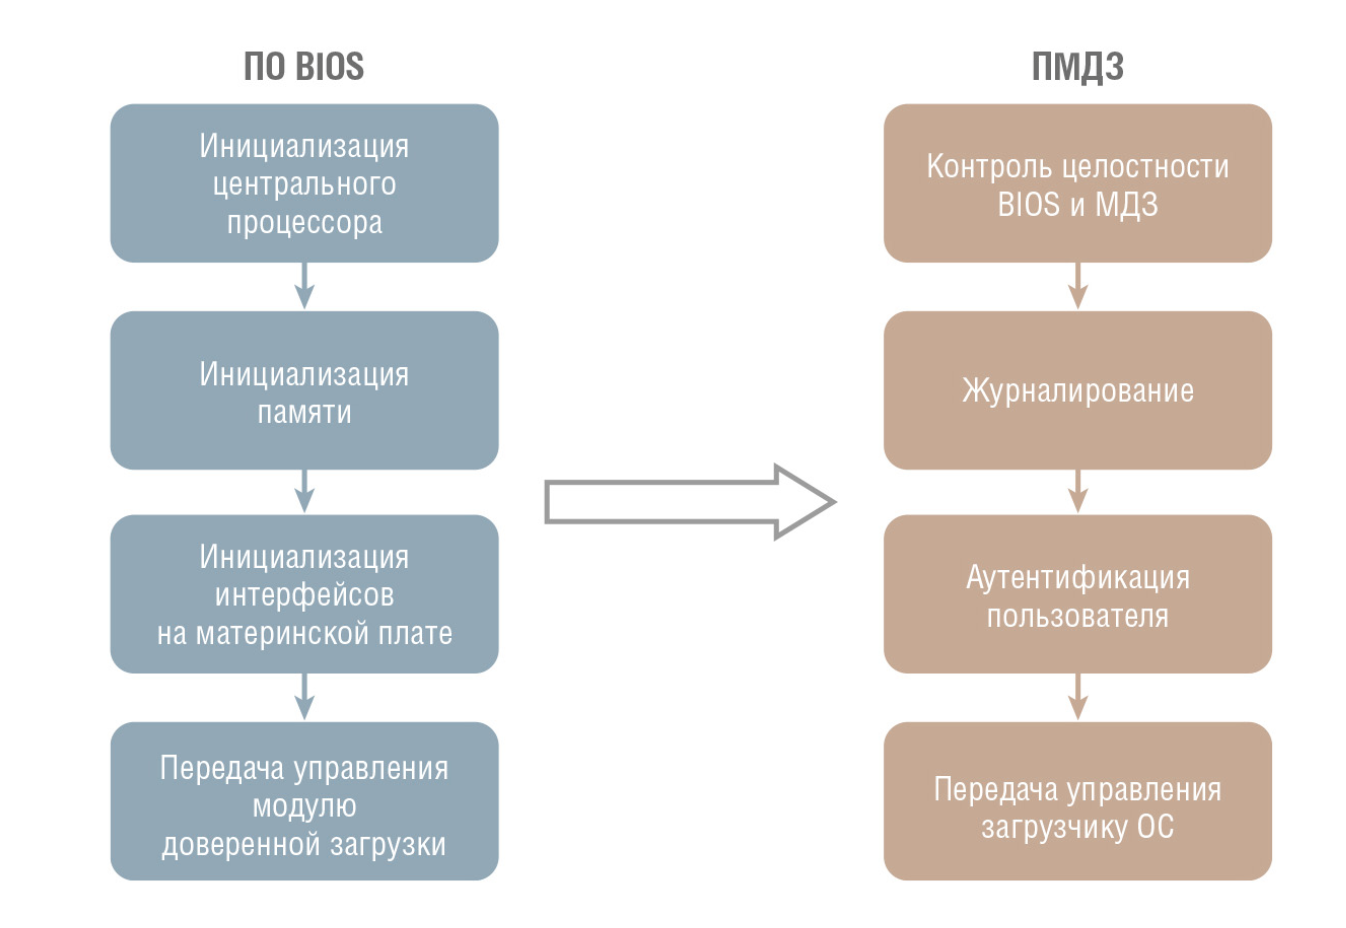
\includegraphics[width=1\textwidth]{pict/8}
  \caption{Общий алгоритм работы ПО BIOS c функциями ПМДЗ}
  \label{fig:55}
\end{figure}

Данный подход позволяет устранить недостатки предыдущих решений и реализовать надежную и эффективную систему доверенной загрузки, интегрированную на низком уровне в базовое программное обеспечение вычислительной платформы.

Модули доверенной загрузки осуществляют верификацию контрольных сумм и других 
характеристик загружаемых данных, сравнивая их с некоторыми уже известными значениями. Таким образом обеспечивается надежный контроль целостности 
программного обеспечения еще до того, как оно будет фактически запущено. Это 
является ключевым фактором защиты от широкого спектра угроз, связанных с загрузкой 
вредоносных модификаций.

Применение средств доверенной загрузки, которые интегрированы в аппаратные платформы или
реализованы в виде отдельных программно-аппаратных устройств, позволяет повысить
уровень информационной безопасности критически важных систем, снизив риски успешных 
атак на этапе загрузки операционной системы.


\newpage
\subsection{Отечественные решения}
На российском рынке представлено множество решений этого класса, каждое из которых
обладает своим набором возможностей и характеристик. Рассмотрим несколько вариантов данных решений:

\subsubsection{«Аккорд-АМДЗ»}
Средство доверенной загрузки уровня платы расширения «Аккорд-АМДЗ» – разработка 
компании «ОКБ САПР» [3]. 

\begin{figure}[H]
  \centering
  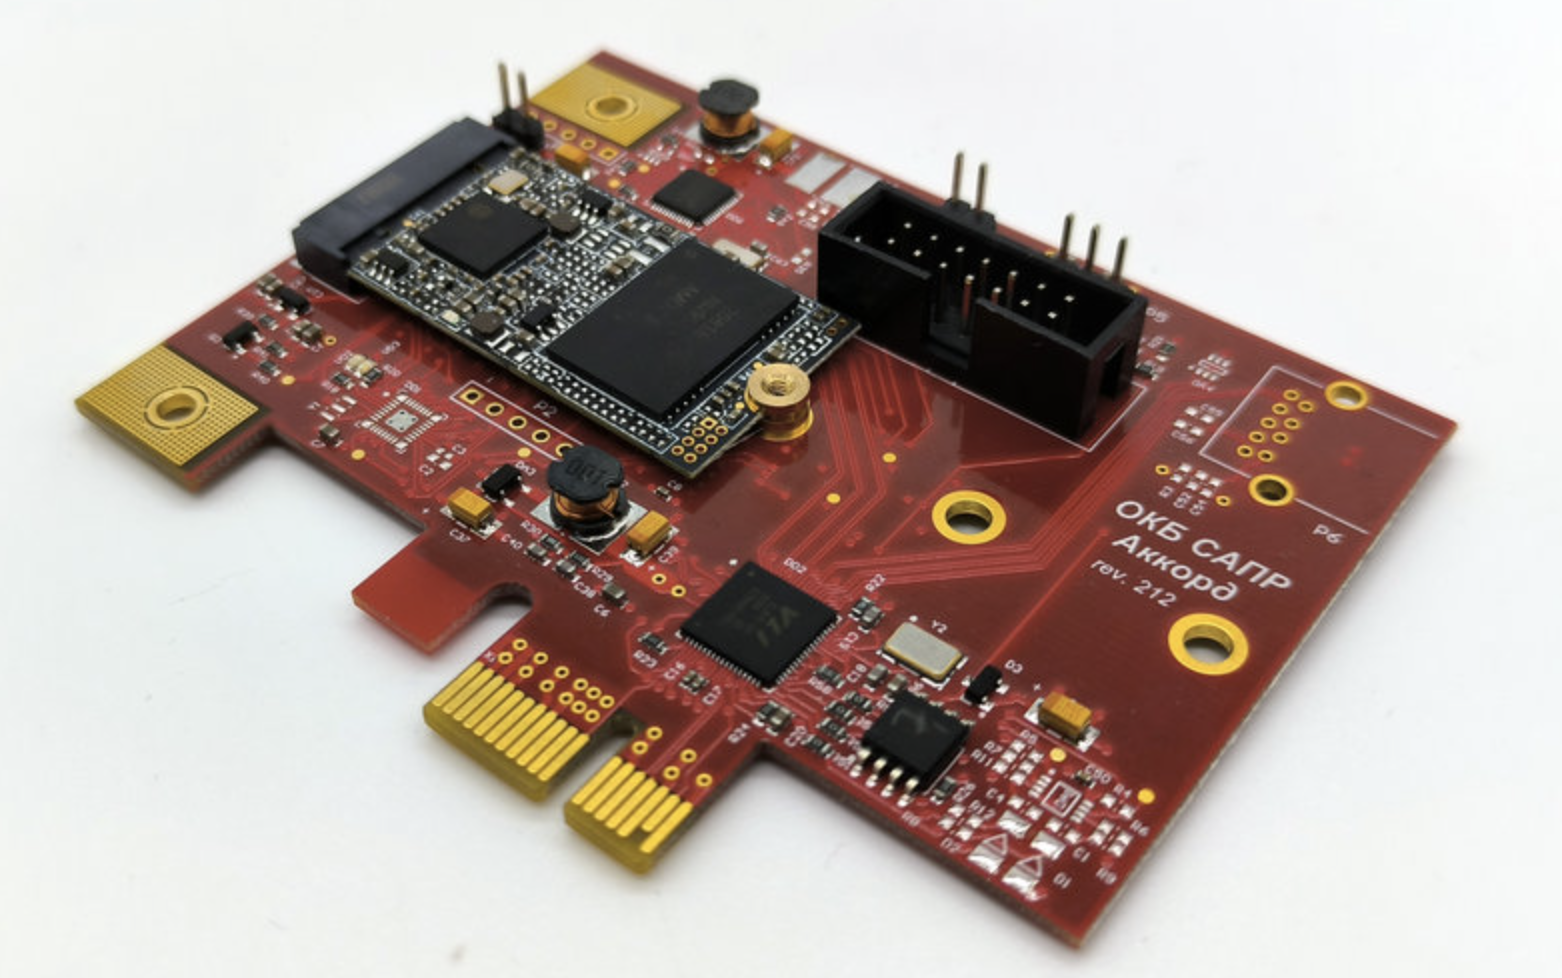
\includegraphics[width=1\textwidth]{pict/17}
  \caption{Аппаратный модуль «Аккорд-АМДЗ»}
  \label{fig:60}
\end{figure}


«Аккорд-АМДЗ» "--- это аппаратный модуль доверенной загрузки
для IBM-совместимых ПК серверов и рабочих станций корпоративной сети. Продукт 
«ОКБ САПР» соответствует концепции резидентного компонента безопасности. Это 
автономное примитивное устройство с защищенной памятью, которое способно влиять 
на архитектуру старта устройства.

Данный защитный комплекс, включающий в себя специализированный
контроллер с предустановленной операционной средой. Помимо этого, 
СДЗ распространяется вместе с функциональным программным обеспечением. Оба этих
составляющих еще на этапе изготовления становятся частью единого резидентного ПО, 
размещенного в энергонезависимой флеш-памяти контроллера.

Комплекс создает доверенную среду для работы программ, обеспечивающих защиту 
на всех шагах (Рис. 3).

\begin{figure}[H]
  \centering
  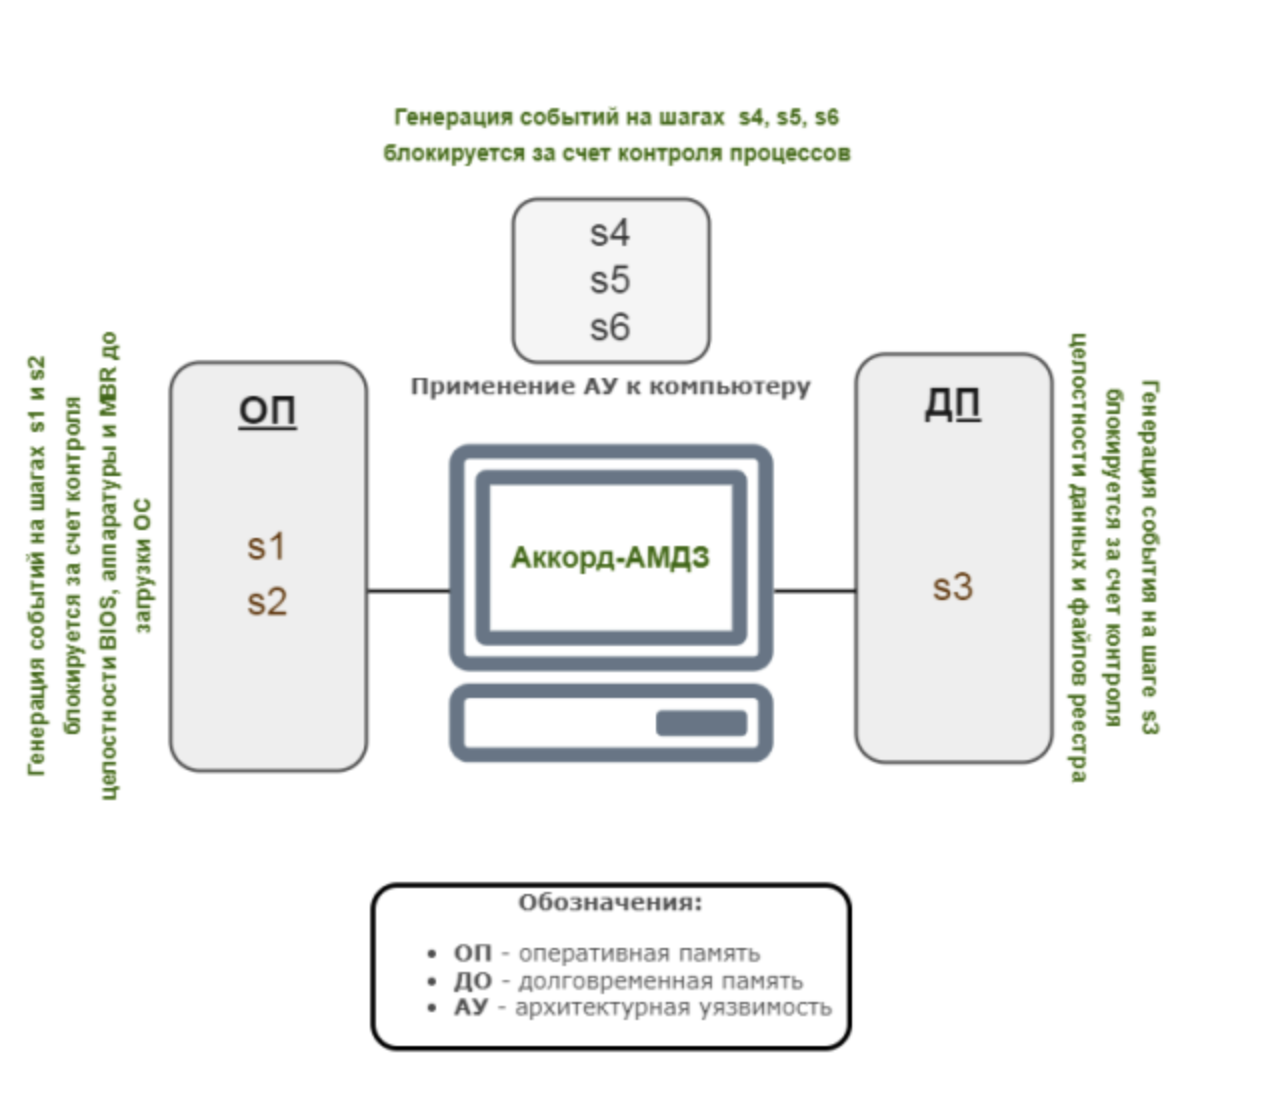
\includegraphics[width=1\textwidth]{pict/9}
  \caption{Работа комплекса}
  \label{fig:56}
\end{figure}


Помимо этого, «Аккорд-АМДЗ» обеспечивает:
\begin{itemize}
  \item[--] защиту ресурсов СВТ от лиц, не допущенных к работе на ней;
  \item[--] аутентификацию пользователей с защитой от раскрытия пароля до загрузки ОС;
  \item[--] блокировку загрузки с внешних носителей;
  \item[--] контроль целостности технических, программных средств и объектов файловых систем, размещенных на динамических дисках;
  \item[--] доверенную загрузку системного и прикладного ПО;
  \item[--] регистрацию контролируемых событий в системном журнале, размещенном в энергонезависимой памяти контроллера;
  \item[--] возможность физической коммутации управляющих сигналов периферийных устройств;
  \item[--] администрирование встроенного ПО комплекса;
  \item[--] регистрацию, сбор, хранение и выдачу данных о событиях, происходящих в СВТ в части системы защиты от несанкционированного доступа.
\end{itemize}

У «Аккорд-АМДЗ» есть сертификаты образцов ФСТЭК. Также это СДЗ входит в реестр отечественного ПО.

\subsubsection{ПАК «Соболь»}
«Соболь» "--- аппаратно-программный модуль доверенной загрузки, функционирующий в среде UEFI. 
Электронный замок «Соболь» предназначен для защиты персональных компьютеров, 
специализированных устройств и серверов в их классическом понимании. Продукт компании 
«Код Безопасности» позволяет вести контроль неизменности файловых систем: NTFS, FAT16,
 FAT32, EXT2, EXT3, EXT4 в операционных системах Linux и Windows [4].

 \begin{figure}[H]
  \centering
  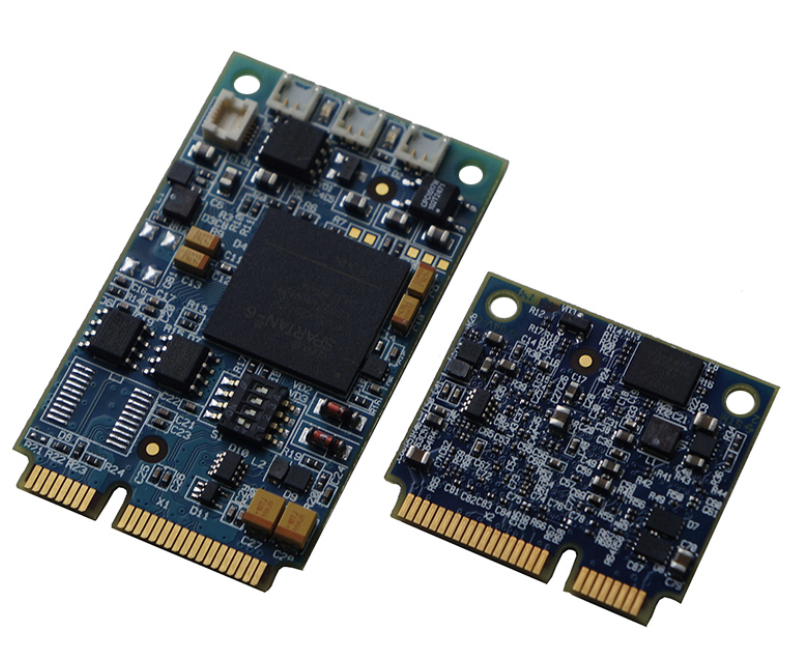
\includegraphics[width=1\textwidth]{pict/15}
  \caption{Аппаратный модуль ПАК «Соболь»}
  \label{fig:61}
\end{figure}


ПАК «Соболь» по заявлениям компании-разработчика создан для решения четырех ключевых задач:
\begin{itemize}
  \item [--] контроль целостности компонентов ИС;
  \item [--] запрет загрузки ОС с внешних носителей;
  \item [--] защита конфиденциальной информации и гостайны в соответствии с требованиями нормативных документов;
  \item [--] защита информации от несанкционированного доступа.
\end{itemize}

\begin{figure}[H]
  \centering
  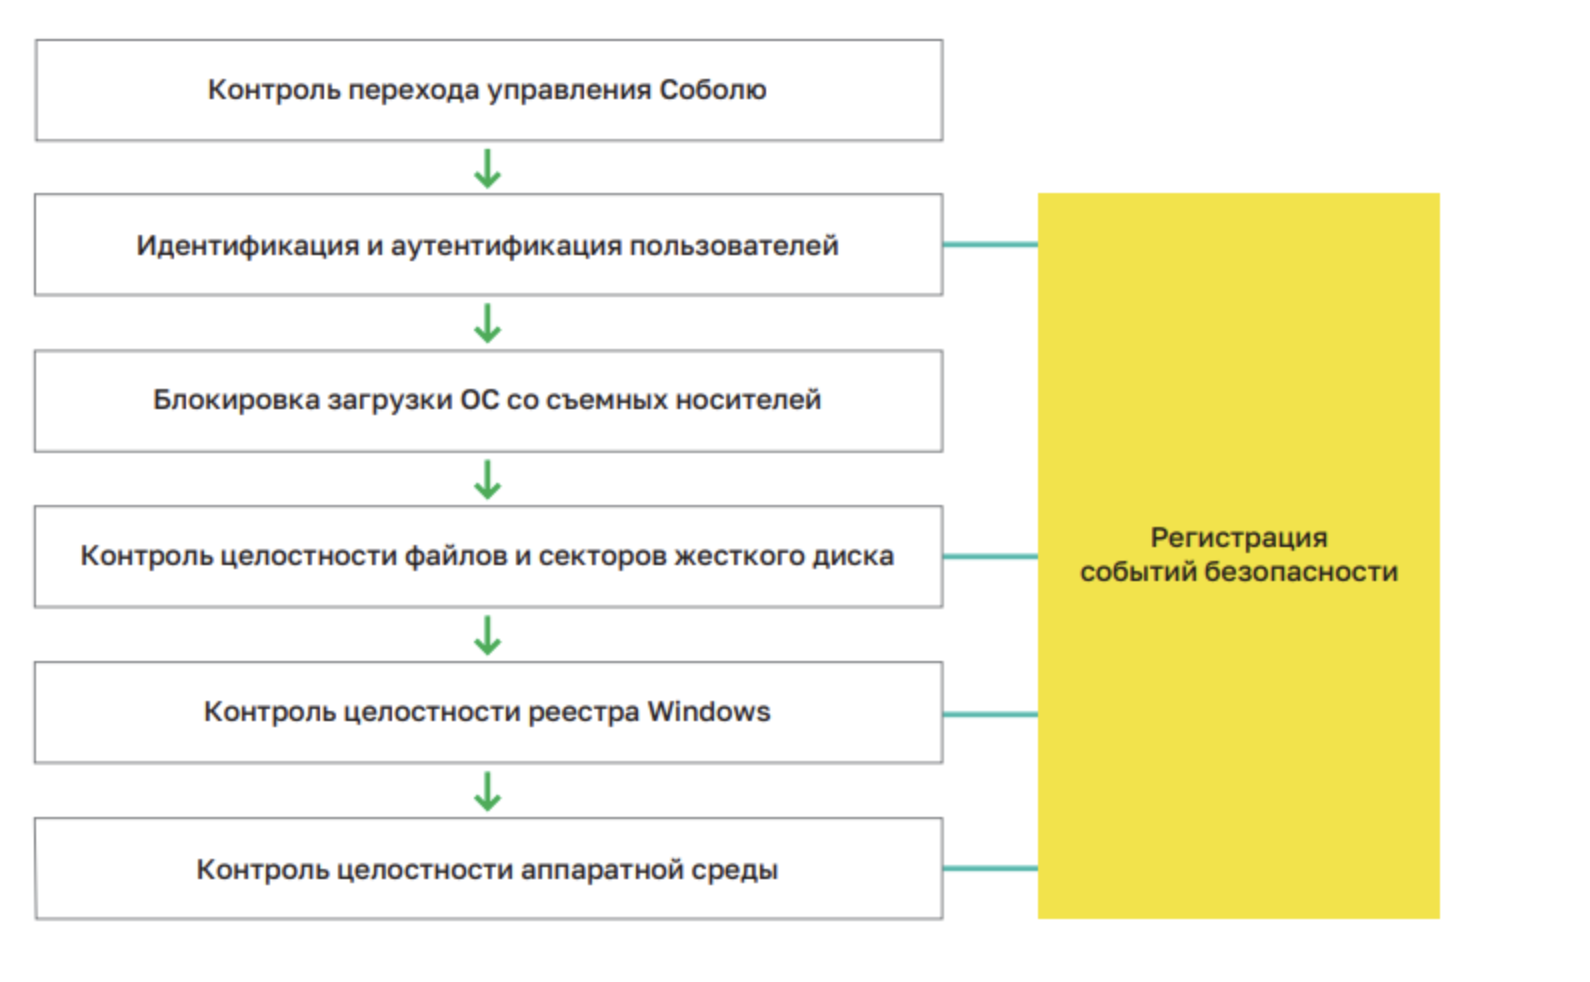
\includegraphics[width=1\textwidth]{pict/11}
  \caption{Принцип работы модуля}
  \label{fig:57}
\end{figure}


Среди интересных преимуществ ПАК «Соболь» можно отметить наличие «сторожевого таймера». 
С его помощью СДЗ блокирует доступ к компьютеру, если управление при его включении 
не передано ПАК «Соболь». Вся информация о попытках входа в систему записывается 
устройством в журнал, который хранится в энергонезависимой памяти. Журнал фиксирует 
не только сам факт входа в систему, но и имя пользователя, предъявление незарегистрированных 
идентификаторов, неправильные вводы пароля, а также дату и время регистрации этих событий.
 Таким образом «Соболь» позволяет компании применить дополнительные меры защиты информации
 при обнаружении несанкционированных попыток входа в систему.

ПАК «Соболь» входит в реестр отечественного ПО. Также продукт имеет сертификаты соответствия
требованиям ФСТЭК и ФСБ.



\subsubsection{Dallas Lock}

Несмотря на американский мотив названия, Dallas Lock "--- разработка российской компании 
«Конфидент». Это средство доверенной загрузки представляет собой плату расширения 
для защиты информации. По заявлению «Конфидент», продукт может защищать сведения вплоть 
до уровня «совершенно секретно». Как и другие решения этого типа Dallas Lock ведет журнал 
и проверяет целостность программно-аппаратной среды до загрузки операционной системы [5].

\begin{figure}[H]
  \centering
  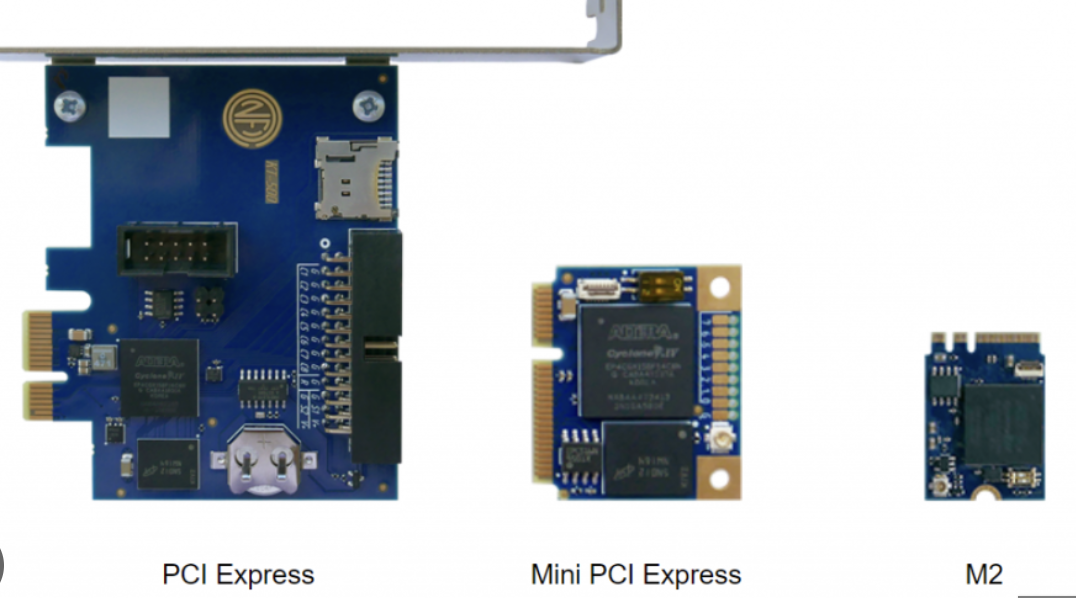
\includegraphics[width=1\textwidth]{pict/14}
  \caption{Аппаратные модули Dallas Lock}
  \label{fig:59}
\end{figure}

Dallas Lock обладает несколькими преимуществами:
\begin{itemize}
  \item[--] администрировать средство доверенной загрузки можно без использования ресурсов загружаемой штатной ОC;
  \item[--] позволяет разграничивать доступ к управлению СДЗ;
  \item[--] СДЗ поддерживает безопасный режим загрузки UEFI;
  \item[--] имеет собственные часы с независимым источником питания;
  \item[--] хранит ключи и служебную информацию в энергонезависимой памяти платы СДЗ;
  \item[--] доступ к СДЗ ограничен после загрузки штатной операционной системы;
\end{itemize}

Решение позволяет использовать двухфакторную аппаратную аутентификацию с популярными USB-ключами и электронными ключами.
\begin{figure}[H]
  \centering
  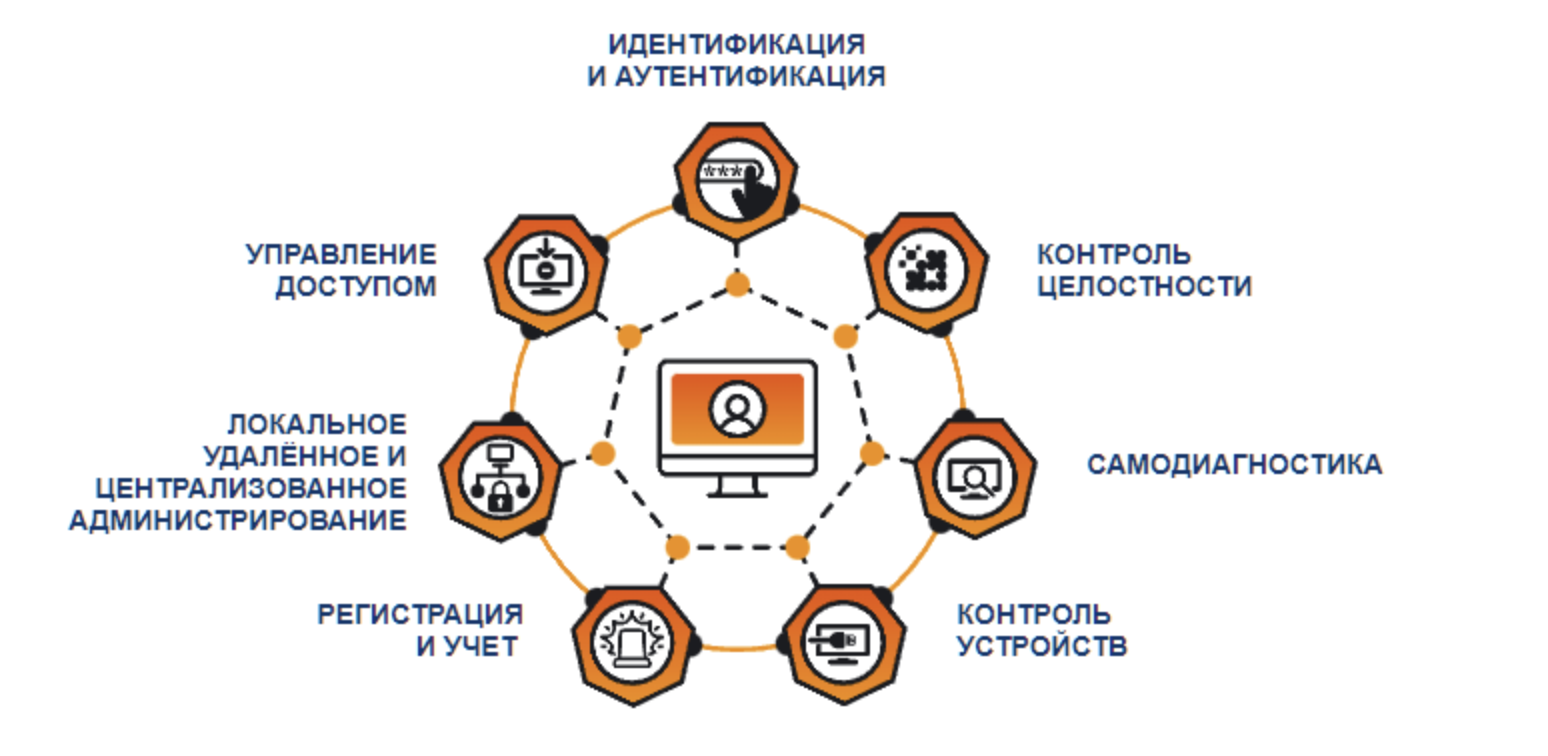
\includegraphics[width=1\textwidth]{pict/12}
  \caption{Комплекс защиты Dallas Lock}
  \label{fig:58}
\end{figure}

СДЗ Dallas Lock входит в реестр отечественного ПО, а также обладает сертификатами ФСТЭК и Минобороны России.

\subsubsection{ViPNet SafeBoot}

Данный продукт разработан российской компанией «ИнфоТеКС». Высокотехнологичный 
программный модуль доверенной загрузки устанавливается в UEFI BIOS. Этот продукт классифицируется как 
СДЗ уровня базовой системы ввода-вывода. ViPNet SafeBoot предназначен для защиты персональных компьютеров, 
мобильных устройств и серверов. Это решение, как и другие, защищает от угрозы несанкционированного 
доступа на этапе загрузки операционной системы [6].

\begin{figure}[H]
  \centering
  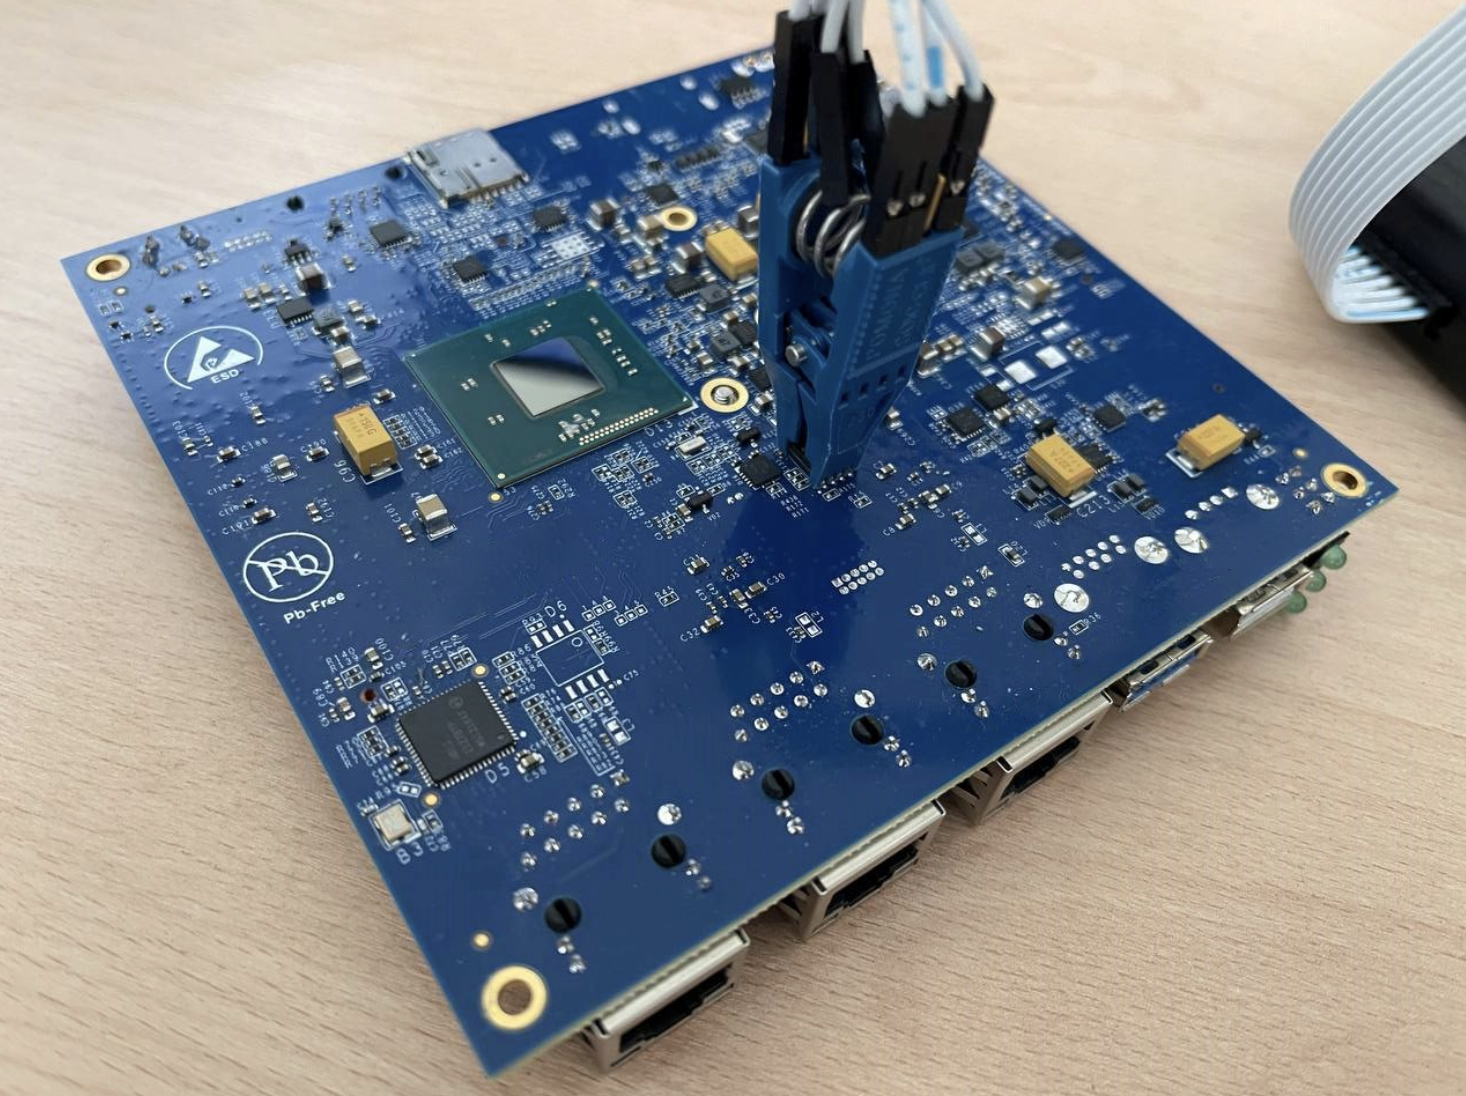
\includegraphics[width=1\textwidth]{pict/13}
  \caption{Аппаратный модуль ViPNet SafeBoot}
  \label{fig:62}
\end{figure}

VipNet SafeBoot обладает несколькими возможностями, среди которых:
\begin{itemize}
  \item [--] авторизация в AD/LDAP;
  \item [--] поддержка SSO для входа в ОС;
  \item [--] защита от вредоносного ПО в BIOS;
  \item [--] ведение журнала событий безопасности;
  \item [--] наличие шаблонов администрирования, позволяющих быстро настроить СДЗ;
  \item [--] защита от обхода и самотестирование;
  \item [--] запрет загрузки с нештатных и внешних носителей;
  \item [--] поддержка двухфакторной аутентификации.
\end{itemize}

Также компания «ИнфоТеКС» среди преимуществ собственного продукта отмечает неизвлекаемость ПМДЗ, 
в отличие от других решений этого класса. VipNet SafeBoot входит в реестр отечественного ПО,
также продукт сертифицирован ФСТЭК России, а значит удовлетворяет требования регуляторов, 
также может быть использовать для построения ИСПДн до У31, ГИС, АСУ ТП и КИИ до 1 класса 
защищенности.




\section{Настройка подсистемы}
\subsection{Вариант}
Вариант №9. Подсистема управления доступом для системы рекрутинговой организации, которая 
обрабатывает ПДн работников и специальные данные 100001 клиентов. 

Определим следующие пункты для составления итогового списка требований:
\begin{itemize}
  \item[1.] класс АC, базовые требования;
  \item[2.] свойства информации;
  \item[3.] класс защищенности СВТ;
  \item[4.] ГИС или ИСПДн; 
  \item[5.] уровень защищенности ИС.
\end{itemize}

%  Определение 
%  -- класс АC, базовые требования (1Г)
%  -- Класс защищенности СВТ (5)
%  -- Определить ГИС или ИСПДн и наверное требования к нему
%  -- Уровень защищенности ИС (2)
 

\subsection{Теоретическая часть}
\subsubsection{Класс АС и базовые требования к подсистеме}
Согласно документу <<Автоматизированные системы. Защита от несанкционированного
доступа к информации. Классификация автоматизированных систем
и требования по защите информации>>, пункт 1.9, система  имеет класс \textbf{1Г} т.к она 
обрабатывает персональные данные и специальные, также является многопользовательской системой с разными полномочиями [7].

В пункт 2.10 документа выделяются следующее базовые требование к подсистемам для данного класса (Рис. 9).

\begin{figure}[H]
  \centering
  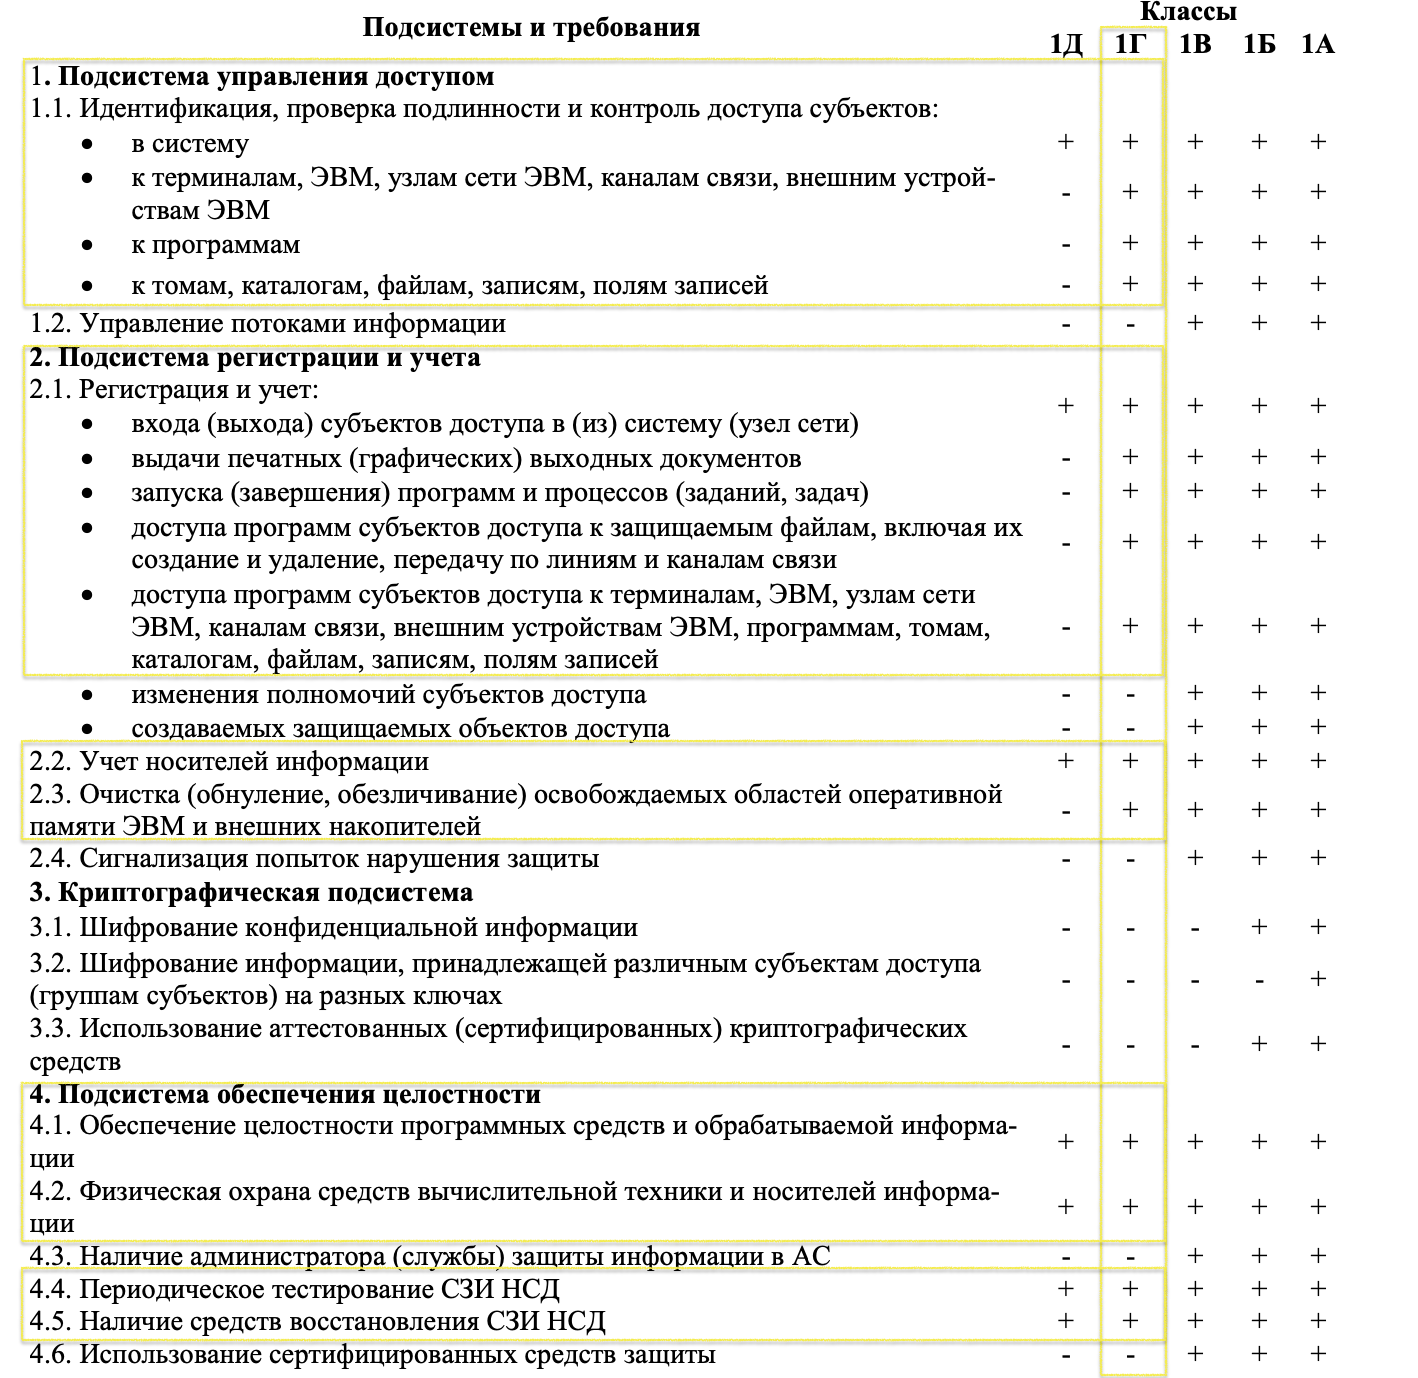
\includegraphics[width=1.1\textwidth]{pict/20}
  \caption{Требования к подсистемам}
  \label{fig:1}
\end{figure}

\textbf{Подсистема управления доступом:}
\begin{itemize}
  \item[--] должна осуществляться идентификация и проверка подлинности субъектов доступа при входе в систему по идентификатору 
  (коду) и паролю условно-постоянного действия, длиной не менее шести буквенно-цифровых символов;
  \item[--] должна осуществляться идентификация терминалов, ЭВМ, узлов сети ЭВМ, каналов связи, внешних устройств ЭВМ по логическим именам;
  \item[--] должна осуществляться идентификация программ, томов, каталогов, файлов, записей, полей записей по именам;
  \item[--] должен осуществляться контроль доступа субъектов к защищаемым ресурсам в соответствии с матрицей доступа.
\end{itemize}
\textbf{Подсистема регистрации и учета:}

Должна осуществляться регистрация входа (выхода) субъектов доступа в
систему (из системы), либо регистрация загрузки и инициализации
операционной системы и ее программного останова. Регистрация выхода из
системы или останова не проводится в моменты аппаратурного отключения
АС. В параметрах регистрации указываются:
\begin{itemize}
  \item[--] дата и время входа (выхода) субъекта доступа в систему (из системы) или
  загрузки (останова) системы;
  \item[--] результат попытки входа: успешная или неуспешная - несанкционированная;
  \item[--] идентификатор (код или фамилия) субъекта, предъявленный при попытке
  доступа;
  \item[--] код или пароль, предъявленный при неуспешной попытке;
  \item[--] должна осуществляться регистрация выдачи печатных (графических) 
  документов на "твердую" копию. В параметрах регистрации указываются:
  дата и время выдачи (обращения к подсистеме вывода);
  спецификация устройства выдачи [логическое имя (номер) внешнего устройства]; 
  краткое содержание (наименование, вид, шифр, код) и уровень конфиденциальности
  документа;
  идентификатор субъекта доступа, запросившего документ;
  \item[--] должна осуществляться регистрация запуска (завершения) программ и процессов
  (заданий, задач), предназначенных для обработки защищаемых файлов. В параметрах 
  регистрации указываются: дата и время запуска, имя (идентификатор) программы (процесса, задания),
  идентификатор субъекта доступа, запросившего программу (процесс, задание), результат запуска (успешный, неуспешный - несанкционированный);
  \item[--] должна осуществляться регистрация попыток доступа средств 
  к защищаемым файлам. В параметрах регистрации указываются: дата и время попытки 
  доступа к защищаемому файлу с указанием ее результата: успешная, неуспешная - несанкционированная,
  идентификатор субъекта доступа, спецификация защищаемого файла;
  \item[--] должна осуществляться регистрация попыток доступа средств к следующим 
  дополнительным защищаемым объектам доступа: терминалам, ЭВМ, узлам сети ЭВМ, линиям (каналам) связи, 
  внешним устройствам ЭВМ, программам, томам, каталогам, файлам, записям, полям записей. В параметрах регистрации указываются:
  дата и время попытки доступа к защищаемому объекту с указанием ее результата: успешная, неуспешная - несанкционированная;
  идентификатор субъекта доступа;
  спецификация защищаемого объекта [логическое имя (номер)];
  \item[--] должен проводиться учет всех защищаемых носителей информации с помощью их
  маркировки и с занесением учетных данных в журнал (учетную карточку);
  \item[--] учет защищаемых носителей должен проводиться в журнале (картотеке) с регистрацией
   их выдачи (приема);
  \item[--] должна осуществляться очистка (обнуление, обезличивание) освобождаемых 
  областей оперативной памяти ЭВМ и внешних накопителей. Очистка осуществляется однократной 
  произвольной записью в освобождаемую область памяти, ранее использованную для хранения 
  защищаемых данных (файлов);
\end{itemize}

\textbf{Подсистема обеспечения целостности:}

Должна быть обеспечена целостность программных средств СЗИ НСД,
обрабатываемой информации, а также неизменность программной среды. При этом:

\begin{itemize}
  \item[--] целостность СЗИ НСД проверяется при загрузке системы по контрольным
  суммам компонент СЗИ;
  \item[--] целостность программной среды обеспечивается использованием
  трансляторов с языков высокого уровня и отсутствием средств модификации
  объектного кода программ в процессе обработки и (или) хранения
  защищаемой информации;
  \item[--] должна осуществляться физическая охрана СВТ (устройств и носителей
  информации), предусматривающая контроль доступа в помещения АС
  посторонних лиц, наличие надежных препятствий для несанкционированного
  проникновения в помещения АС и хранилище носителей информации,
  особенно в нерабочее время;
  \item[--] должно проводиться периодическое тестирование функций СЗИ НСД при
  изменении программной среды и персонала АС с помощью тест-программ,
  имитирующих попытки НСД;
  \item[--] должны быть в наличии средства восстановления СЗИ НСД,
  предусматривающие ведение двух копий программных средств СЗИ НСД и
  их периодическое обновление и контроль работоспособности.
\end{itemize}

\subsubsection{Свойства информции}

Так как система обрабатывает специальные персональные данные пользователей, а также 
данные своих сотрудников, что по Указе Президента РФ от 6 марта 1997 г. № 188 
"Об утверждении перечня сведений конфиденциального характера", персональные данные являются конфиденциальной информацией 
и должны защищаться, поэтому вместе с целостностью и доступностью необходимо обеспечить конфиденциальность [8].

\subsubsection{Класс защищенности СВТ}

Согласно документу <<РУКОВОДЯЩИЙ ДОКУМЕНТ. Средства вычислительной техники.
Защита от несанкционированного доступа к информации. Показатели
защищенности от несанкционированного доступа к информации>>, пункт 2.1.1 можно 
определить \textbf{5} класс защищенности СВТ [9].
Поскольку в отличие от 6 класса, 5 требует наличия контроля целостности средств 
СЗИ, что соответствует требованиям 
из 1.2.1, но в отличие от 4 класса, 5 не требует защиту работы с физическим носителем,
 сопоставления пользователя с устройством и изоляцию модулей (Рис. 10).

\begin{figure}[H]
  \centering
  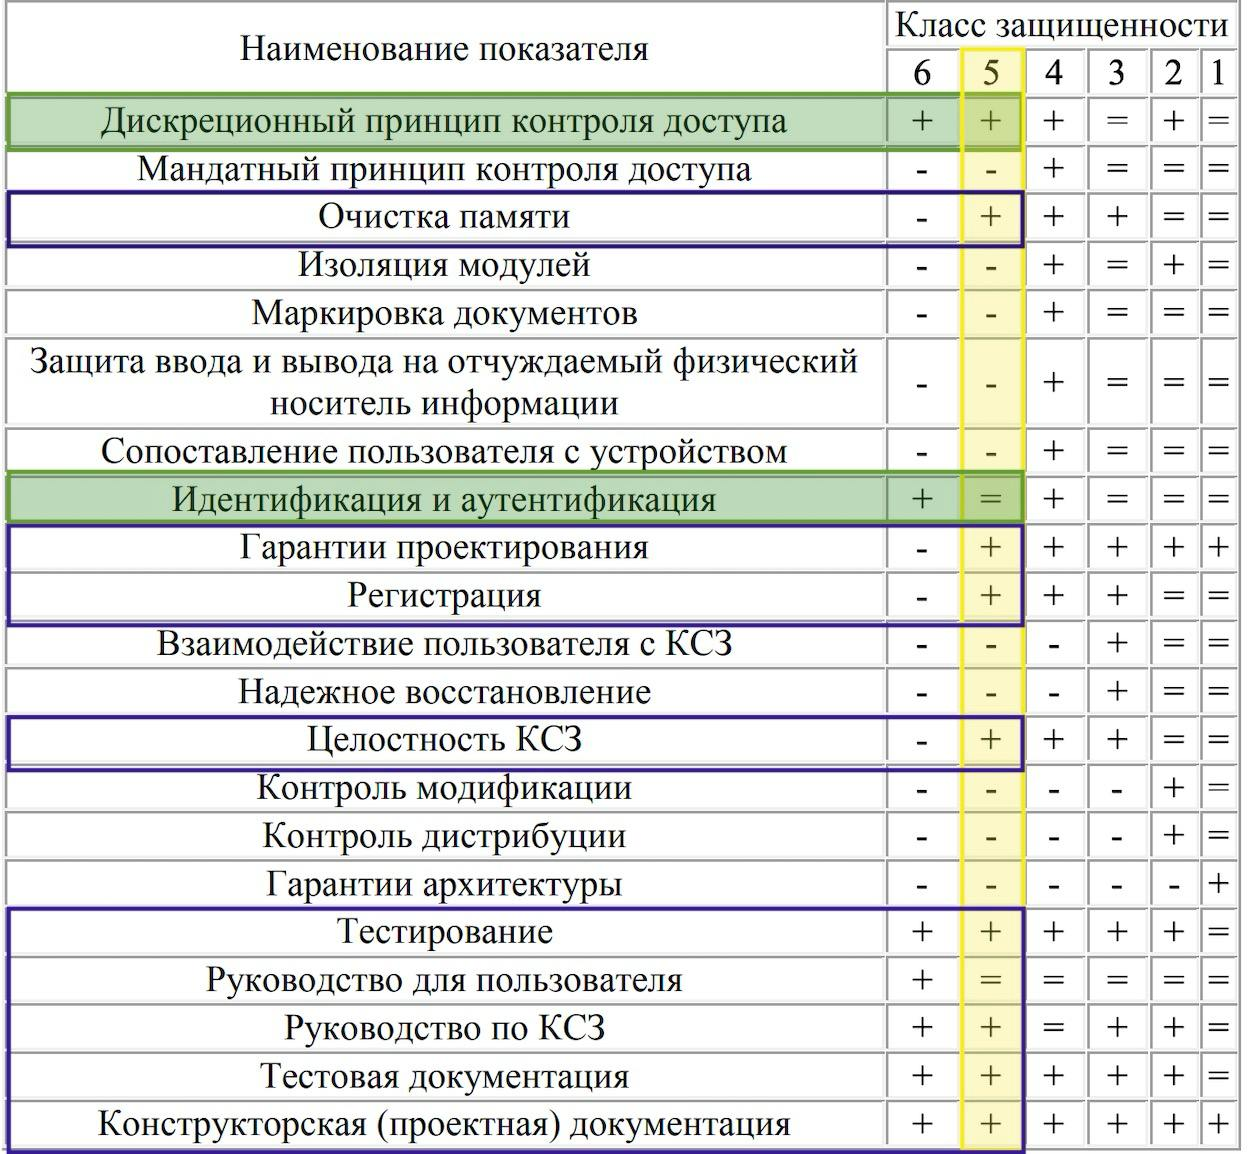
\includegraphics[width=0.7\textwidth]{pict/3}
  \caption{Синий -- требования к системе, зеленый -- к подсистеме управления доступом и идентификации}
  \label{fig:3}
\end{figure}

\textbf{Дискреционный принцип контроля доступа}

КСЗ должен контролировать доступ наименованных субъектов
(пользователей) к наименованным объектам (файлам, программам, томам и
т.д.). Для каждой пары (субъект – объект) в СВТ должно быть задано явное и
недвусмысленное перечисление допустимых типов доступа (читать, писать и
т.д.), т.е. тех типов доступа, которые являются санкционированными для
данного субъекта (индивида или группы индивидов) к данному ресурсу СВТ
(объекту).

КСЗ должен содержать механизм, претворяющий в жизнь дискреционные
правила разграничения доступа.

Контроль доступа должен быть применим к каждому объекту и каждому
субъекту (индивиду или группе равноправных индивидов).

Механизм, реализующий дискреционный принцип контроля доступа,
должен предусматривать возможности санкционированного изменения ПРД,
в том числе возможность санкционированного изменения списка
пользователей СВТ и списка защищаемых объектов.

Права изменять ПРД должны предоставляться выделенным субъектам
(администрации, службе безопасности и т.д.).

Дополнительно должны быть предусмотрены средства управления,
ограничивающие распространение прав на доступ.

\textbf{Очистка памяти}

При первоначальном назначении или при перераспределении внешней
памяти КСЗ должен предотвращать доступ субъекту к остаточной
информации.

\textbf{Идентификация и аутентификация}

КСЗ должен требовать от пользователей идентифицировать себя при
запросах на доступ. КСЗ должен подвергать проверке подлинность
идентификации – осуществлять аутентификацию. КСЗ должен располагать
необходимыми данными для идентификации и аутентификации. КСЗ должен
препятствовать доступу к защищаемым ресурсам неидентифицированных
пользователей и пользователей, подлинность идентификации которых при
аутентификации не подтвердилась.

\textbf{Гарантии проектирования}

На начальном этапе проектирования СВТ должна быть построена модель
защиты. Модель должна включать в себя ПРД к объектам и
непротиворечивые правила изменения ПРД.

\textbf{Регистрация}

КСЗ должен быть в состоянии осуществлять регистрацию следующих
событий:
\begin{itemize}
  \item [--] использование идентификационного и аутентификационного механизма;
  \item [--] запрос на доступ к защищаемому ресурсу (открытие файла, запуск
  программы и т.д.);
  \item [--] создание и уничтожение объекта;
  \item [--] действия по изменению ПРД.
\end{itemize}

Для каждого из этих событий должна регистрироваться следующая
информация:
\begin{itemize}
  \item [--] дата и время;
  \item [--] субъект, осуществляющий регистрируемое действие;
  \item [--] тип события (если регистрируется запрос на доступ, то следует отмечать
   объект и тип доступа);
  \item [--] успешно ли осуществилось событие (обслужен запрос на доступ или нет).
\end{itemize}
КСЗ должен содержать средства выборочного ознакомления с
регистрационной информацией.

\textbf{Целостность КСЗ}

В СВТ пятого класса защищенности должны быть предусмотрены
средства периодического контроля за целостностью программной и
информационной части КСЗ.

\textbf{Тестирование}

В СВТ пятого класса защищенности должны тестироваться:
\begin{itemize}
  \item [--] реализация ПРД (перехват явных и скрытых запросов на доступ,
  правильное распознавание санкционированных и несанкционированных
  запросов, средства защиты механизма разграничения доступа,
  санкционированные изменения ПРД);
  \item [--] успешное осуществление идентификации и аутентификации, а также их
  средства защиты;
  \item [--] очистка памяти в соответствии с п. 2.3.2;
  \item [--] регистрация событий в соответствии с п. 2.3.5, средства защиты
  регистрационной информации и возможность санкционированного 
  ознакомления с ней;
  \item [--] работа механизма, осуществляющего контроль за целостностью КСЗ.
\end{itemize}

\textbf{Руководство пользователя}

Документация на СВТ должна включать в себя краткое руководство для
пользователя с описанием способов использования КСЗ и его интерфейса с
пользователем..

\textbf{Руководство по КСЗ}

Данный документ адресован администратору защиты и должен
содержать:

\begin{itemize}
  \item [--] описание контролируемых функций;
  \item [--] руководство по генерации КСЗ;
  \item [--] описания старта СВТ, процедур проверки правильности старта, процедур
  работы со средствами регистрации.
\end{itemize}


\textbf{Тестовая документация}

Должно быть предоставлено описание тестов и испытаний, которым
подвергалось СВТ (в соответствии с требованиями п.2.3.7), и результатов
тестирования.

\textbf{Конструкторская и проектная документация}

Должна содержать:
\begin{itemize}
  \item [--] описание принципов работы СВТ;
  \item [--] общую схему КСЗ;
  \item [--] описание интерфейсов КСЗ с пользователем и интерфейсов модулей КСЗ;
  \item [--] модель защиты;
  \item [--] описание механизмов контроля целостности КСЗ, очистки памяти,
  идентификации и аутентификации.
\end{itemize}


\subsubsection{ГИС или ИСПДн}

Так как моя организация "---рекрутинговое агентство, система которого обрабатывает специальные ПДн и сотрудников,
что не является государственной информацией, то система является ИСПДн.


\subsubsection{Уровень защищенности ИС}
Согласно постановлению от 1 ноября 2012 г. N 1119 <<ОБ УТВЕРЖДЕНИИ ТРЕБОВАНИЙ
К ЗАЩИТЕ ПЕРСОНАЛЬНЫХ ДАННЫХ ПРИ ИХ ОБРАБОТКЕ В ИНФОРМАЦИОННЫХ СИСТЕМАХ ПЕРСОНАЛЬНЫХ ДАННЫХ>>,
пункт 10, уровень защищенности можно определить как \textbf{УЗ 2} [10]. Так как система
подходит под одно из условий этого уровня, системе не грозят угрозы 1 и 2 класса, т.к используется лицензированное
ПО и ОС (Рис. 11).

\begin{figure}[H]
  \centering
  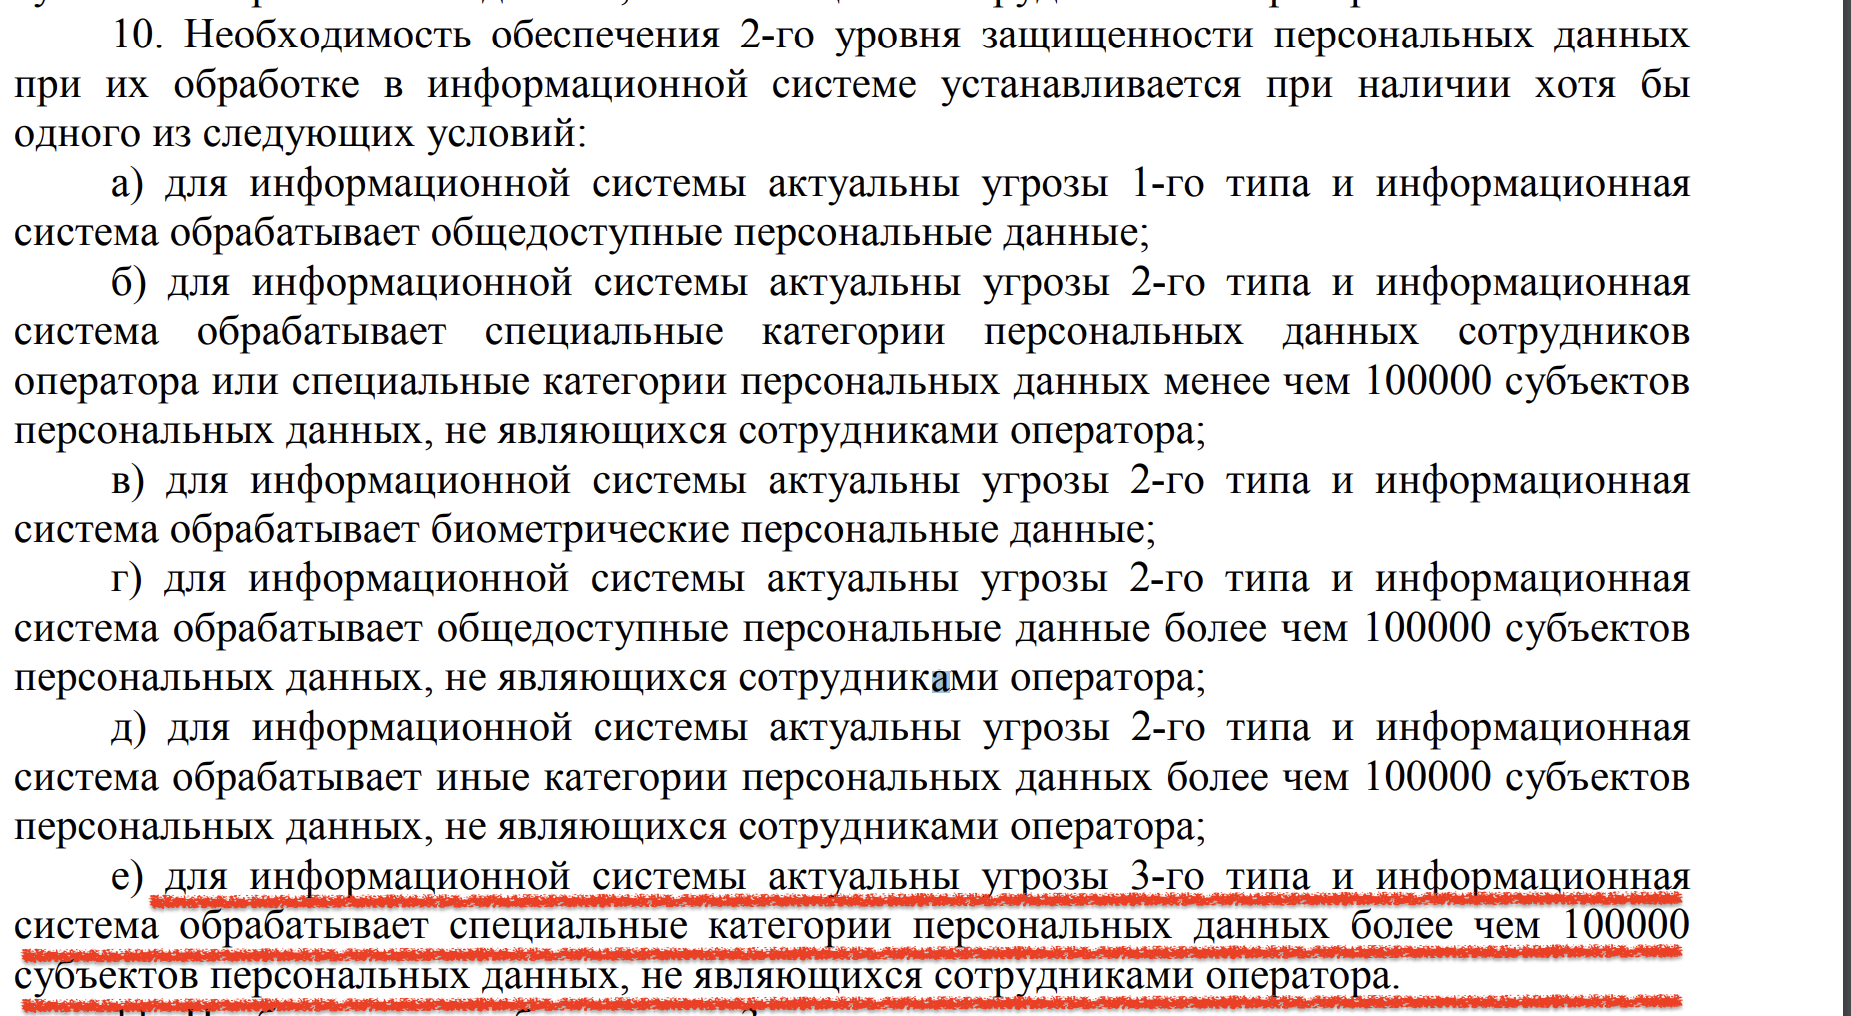
\includegraphics[width=1.1\textwidth]{pict/6}
  \caption{Условия для УЗ 2}
  \label{fig:4}
\end{figure}

Требования, которы выставляются для данного уровня защищенности, пункты 13-15 (Рис. 12). 

\begin{figure}[H]
  \centering
  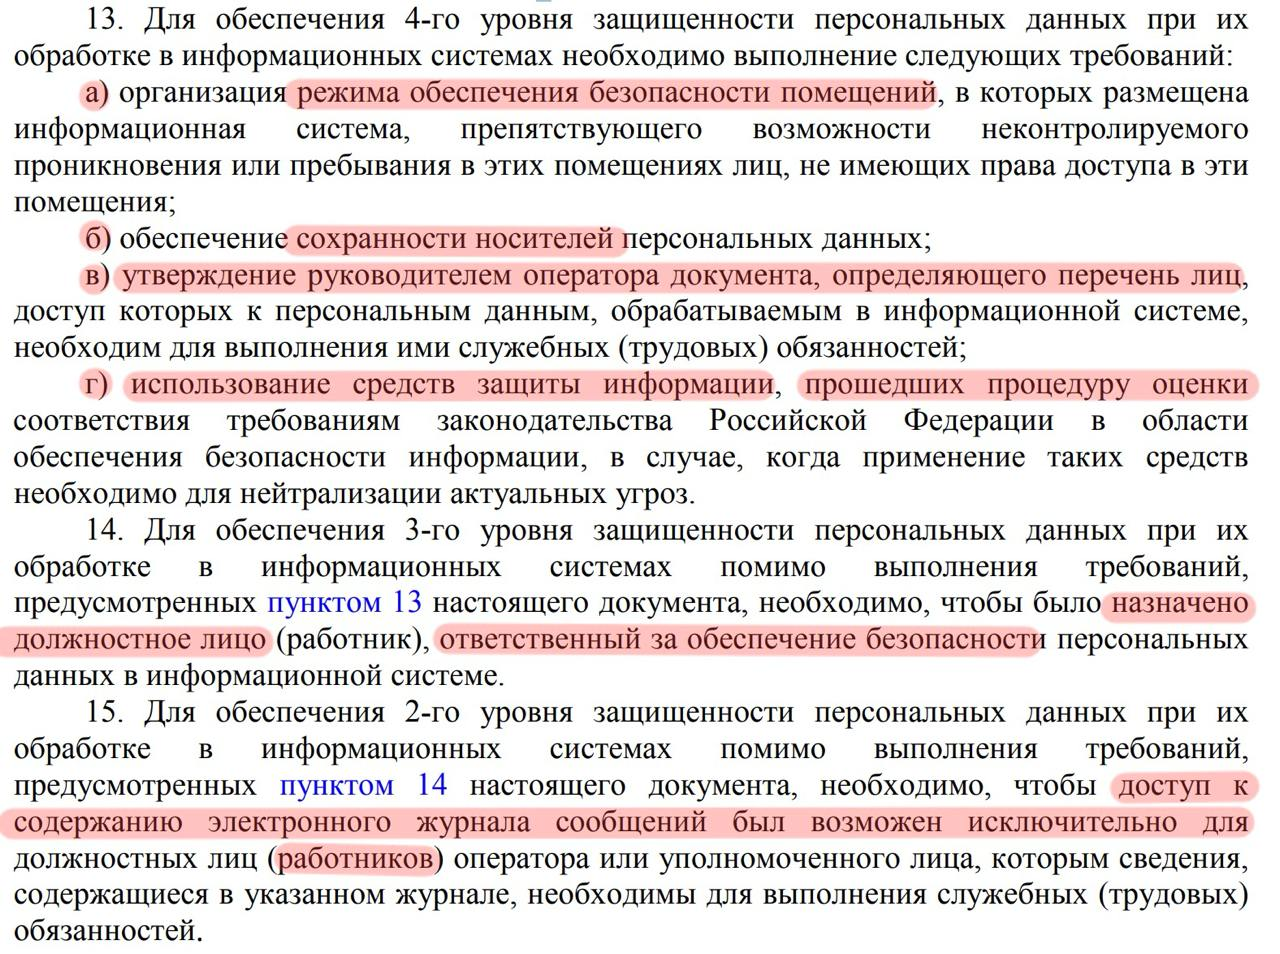
\includegraphics[width=1\textwidth]{pict/5}
  \caption{Требования для УЗ 2}
  \label{fig:5}
\end{figure}

\subsubsection{Требования для подсистемы управления доступом}
По итогу собранных требований, можно выделить список требований конкретно для
подсистемы управления доступом:

\begin{itemize}
  \item[1.] идентификация и проверка подлинности субъектов доступа при входе в систему по идентификатору 
  (коду) и паролю условно-постоянного действия, длиной не менее шести буквенно-цифровых символов;
  \item[2.] идентификация терминалов, ЭВМ, узлов сети ЭВМ, каналов связи, внешних устройств ЭВМ по логическим именам;
  \item[3.] идентификация программ, томов, каталогов, файлов, записей, полей записей по именам;
  \item[4.] контроль доступа субъектов к защищаемым ресурсам в соответствии с матрицей доступа;
  \item[5.] КСЗ должен содержать механизм, претворяющий в жизнь дискреционные
  правила разграничения доступа;
  \item[6.] ограничение прав для пользователей, могут пенять права доступа только админы;
  \item[7.] настройка доступа к электронному журналу сообщений только для субъектов, использующих их в работе.
\end{itemize}
\newpage



1) Управление 
учетными записями пользователей, в том числе внешних пользователей;
5) Ограничение неуспешных попыток входа в информационную
систему (доступа к информационной системе);
6) Блокирование сеанса доступа в информационную систему после
установленного времени бездействия (неактивности) пользователя или по его
запросу;



% Вручную оформление ссылок не допускается

% \begin{figure}[H]
%   \centering
%   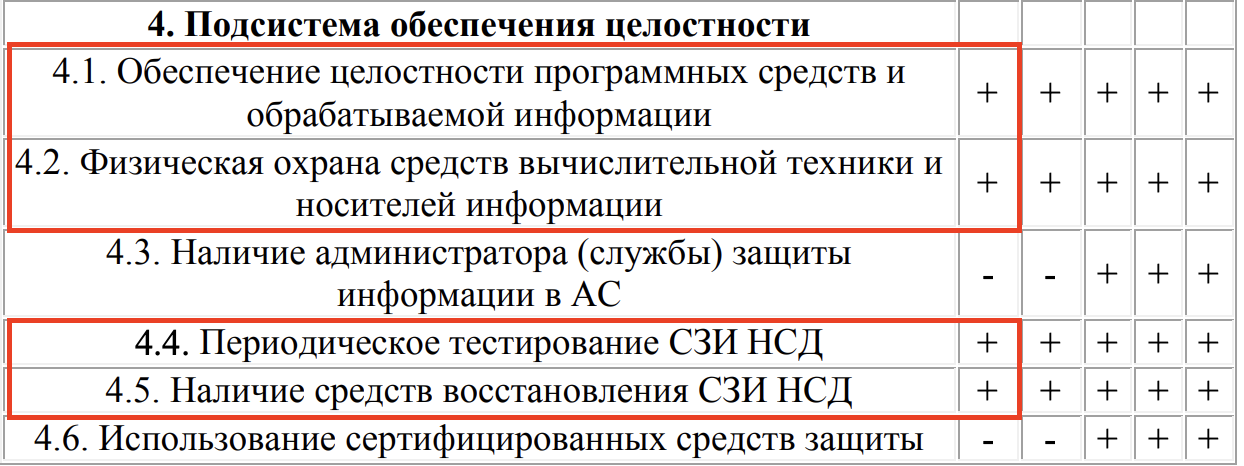
\includegraphics[width=1\textwidth]{pict/2}
%   \caption{принцип взаимодействия уровней приложения}
%   \label{fig:2}
% \end{figure}



\subsection{Практическая часть}
\subsubsection{Настройка доменной системы}
В практике используются виртуальные машины Windows Server 2003 и Windows 10, 
заранее присоединим компьютер к домену, и далее создадим подразделения для
нашей организации соответственно варианту.

Для нашей структуры создадим матрицу доступа субъектов к объектам.
\begin{figure}[H]
  \centering
  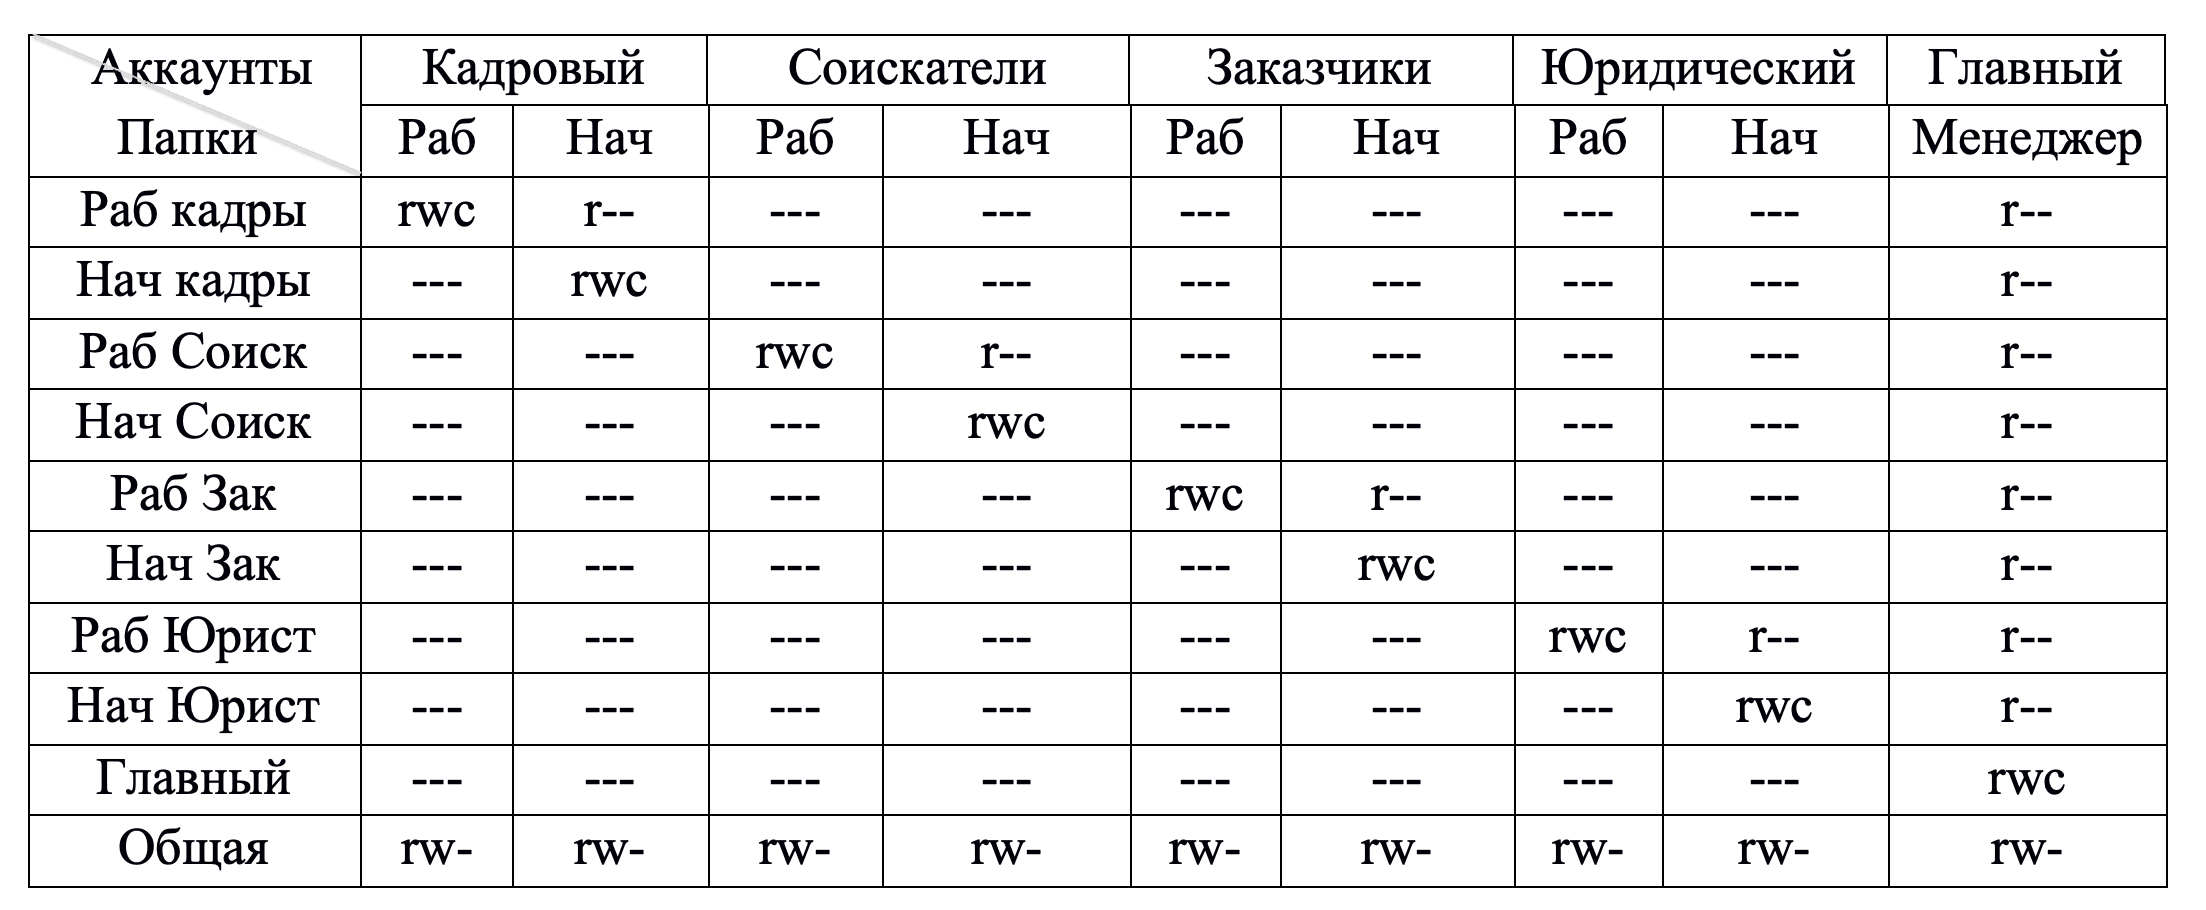
\includegraphics[width=1\textwidth]{pict/102}
  \caption{Матрица доступа, r - чтение, w - запись, c - изменение}
  \label{fig:101}
\end{figure}

\begin{figure}[H]
  \centering
  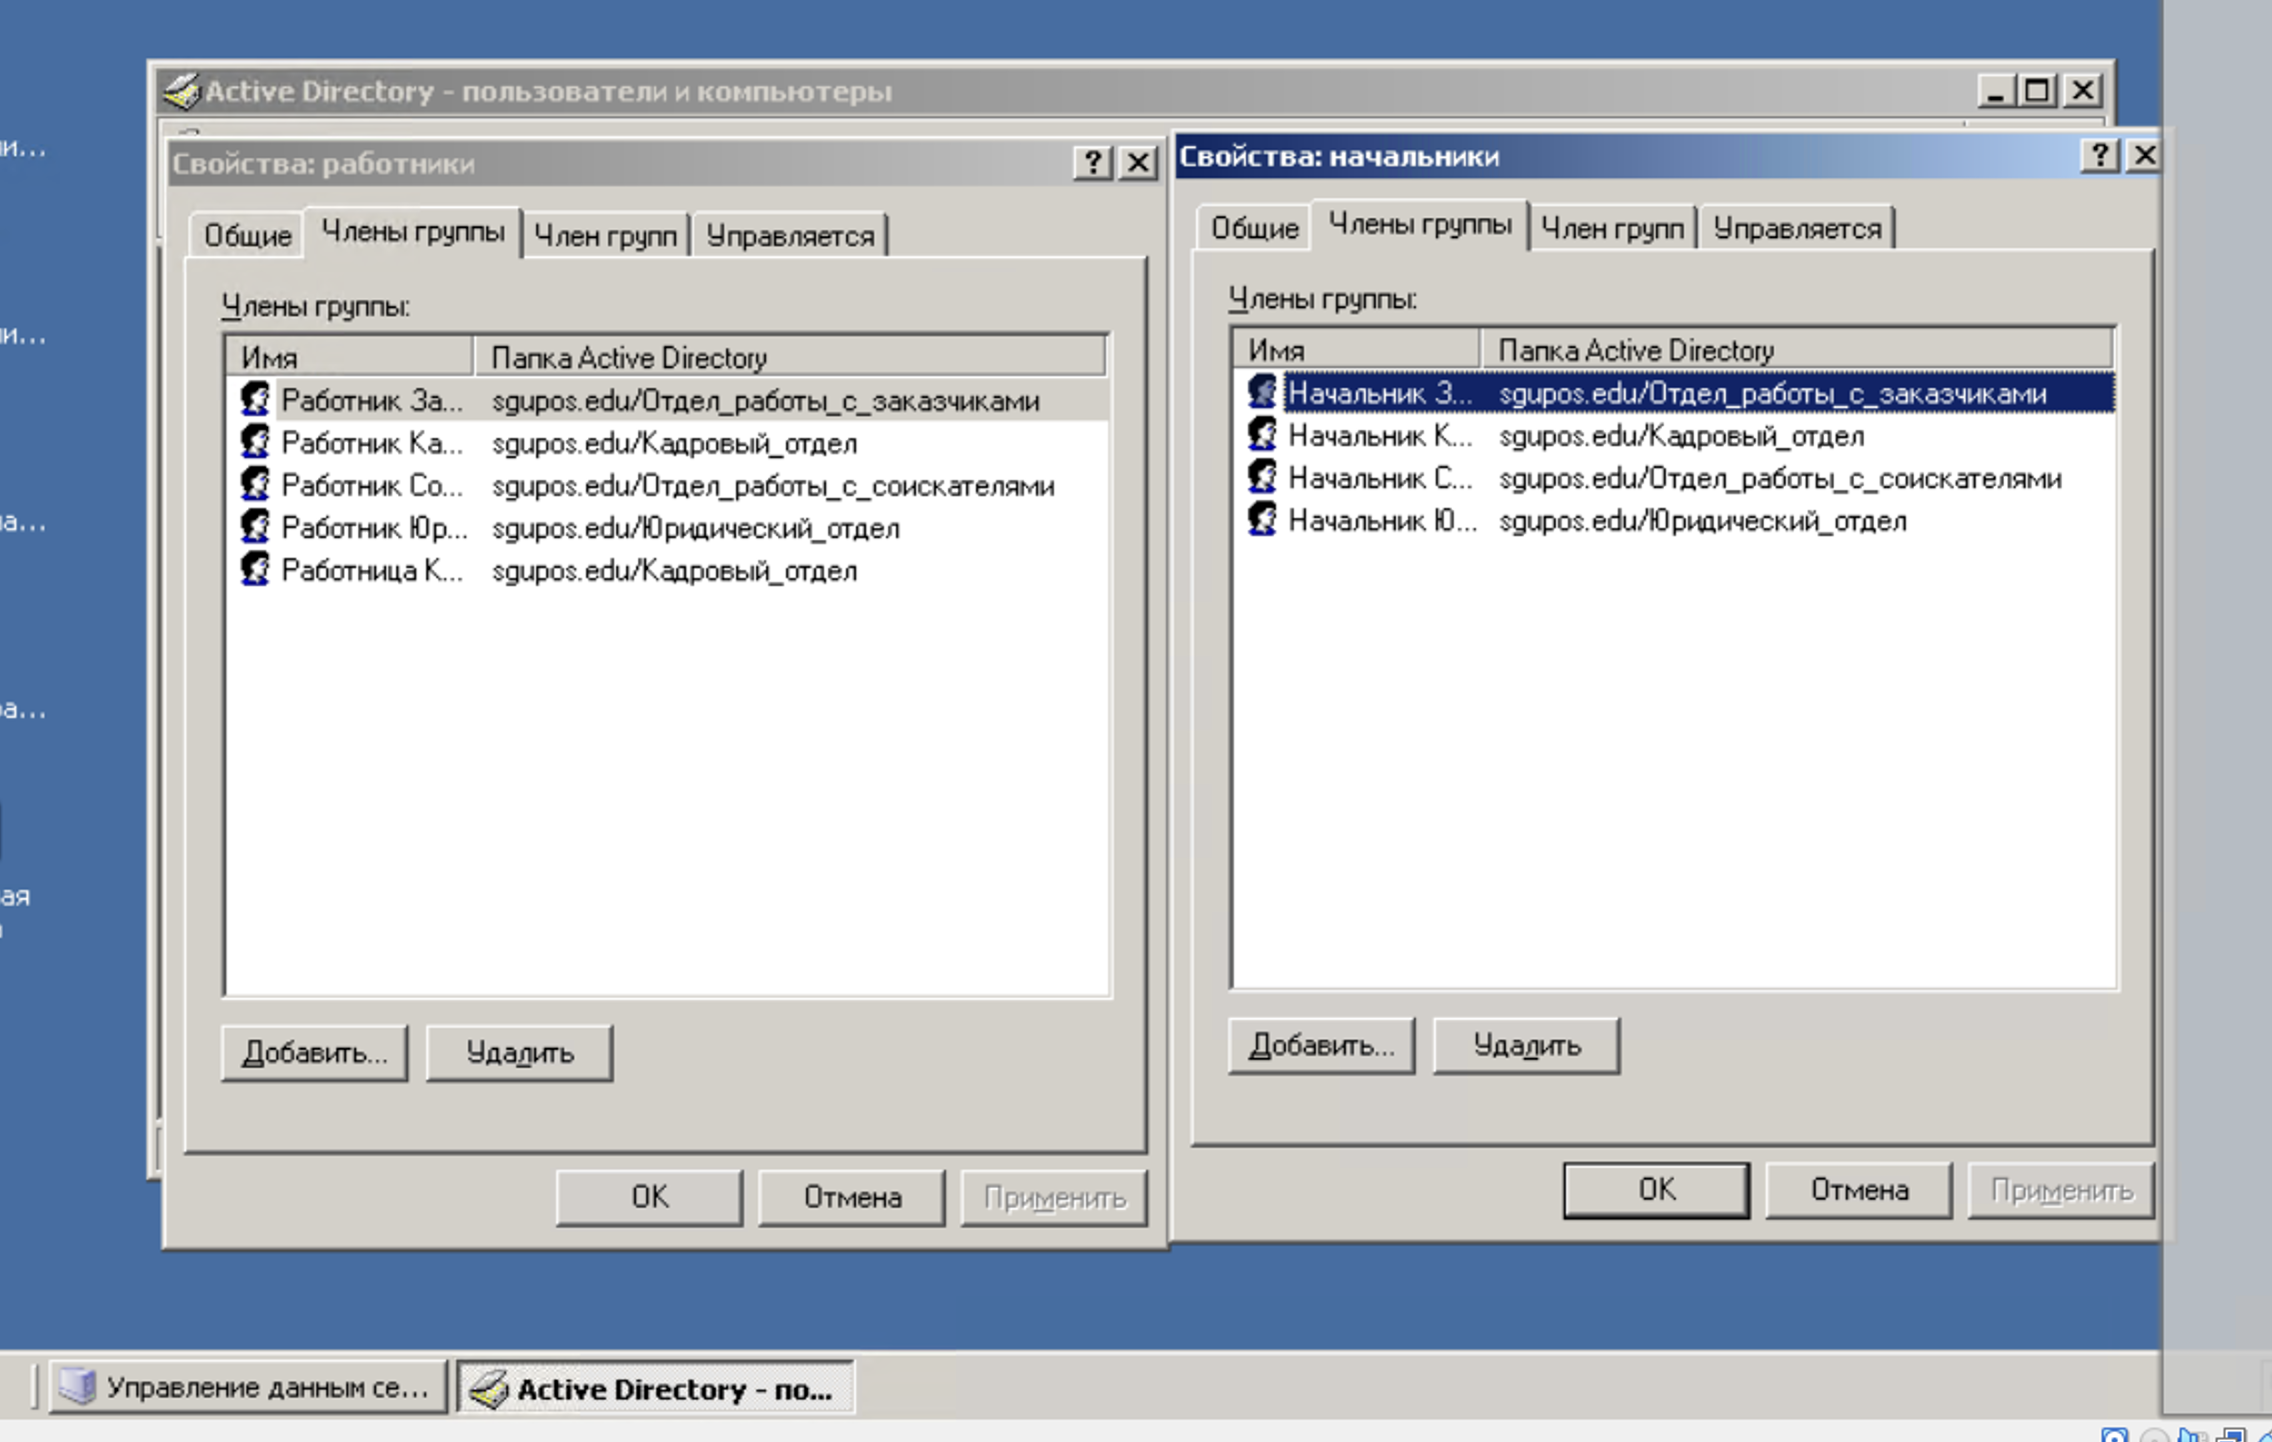
\includegraphics[width=1\textwidth]{pict/prac/54}
  \caption{}
\end{figure}

В домене создадим подразделения соответствующие варианту, а также на одном уровне с ними создадим 
главного пользователя.

\begin{figure}[H]
  \centering
  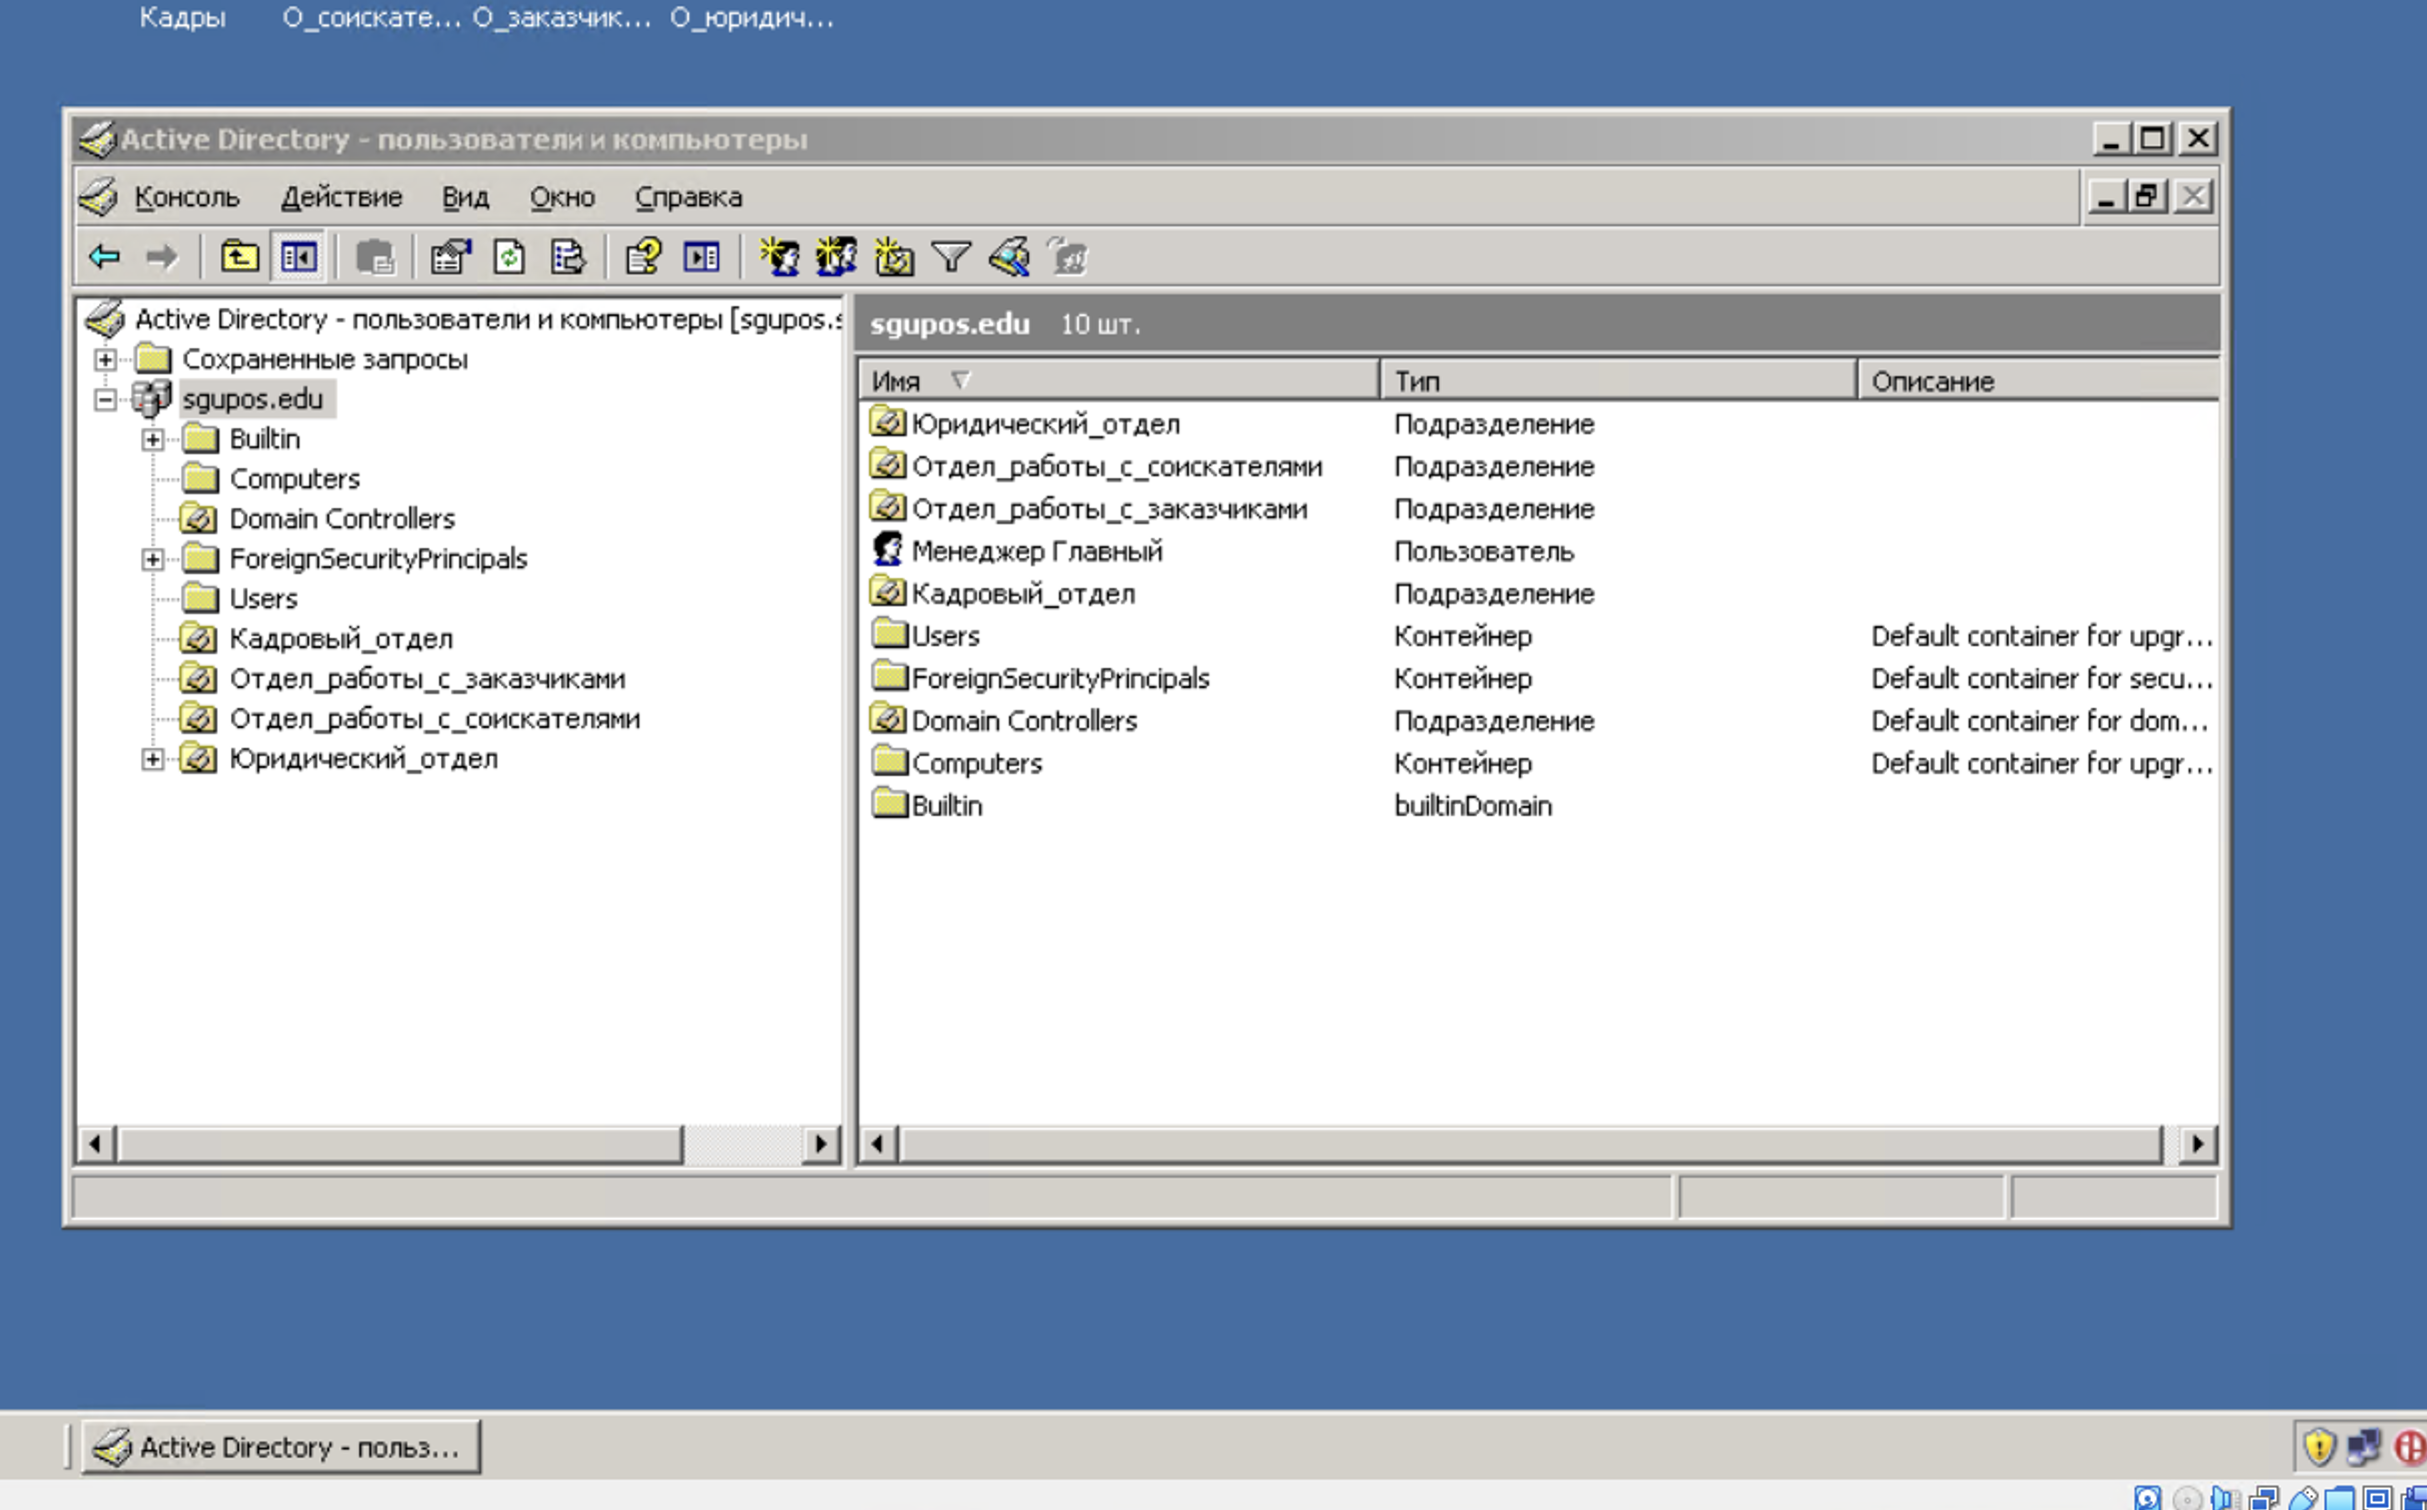
\includegraphics[width=1\textwidth]{pict/prac/3}
  \caption{Подразделения}
  \label{fig:11}
\end{figure}

Одним из требований к классу АС является установка для пользователя пароля длинной не менее 6 
цифро-буквенных символов, включим эту настройку.
\begin{figure}[H]
  \centering
  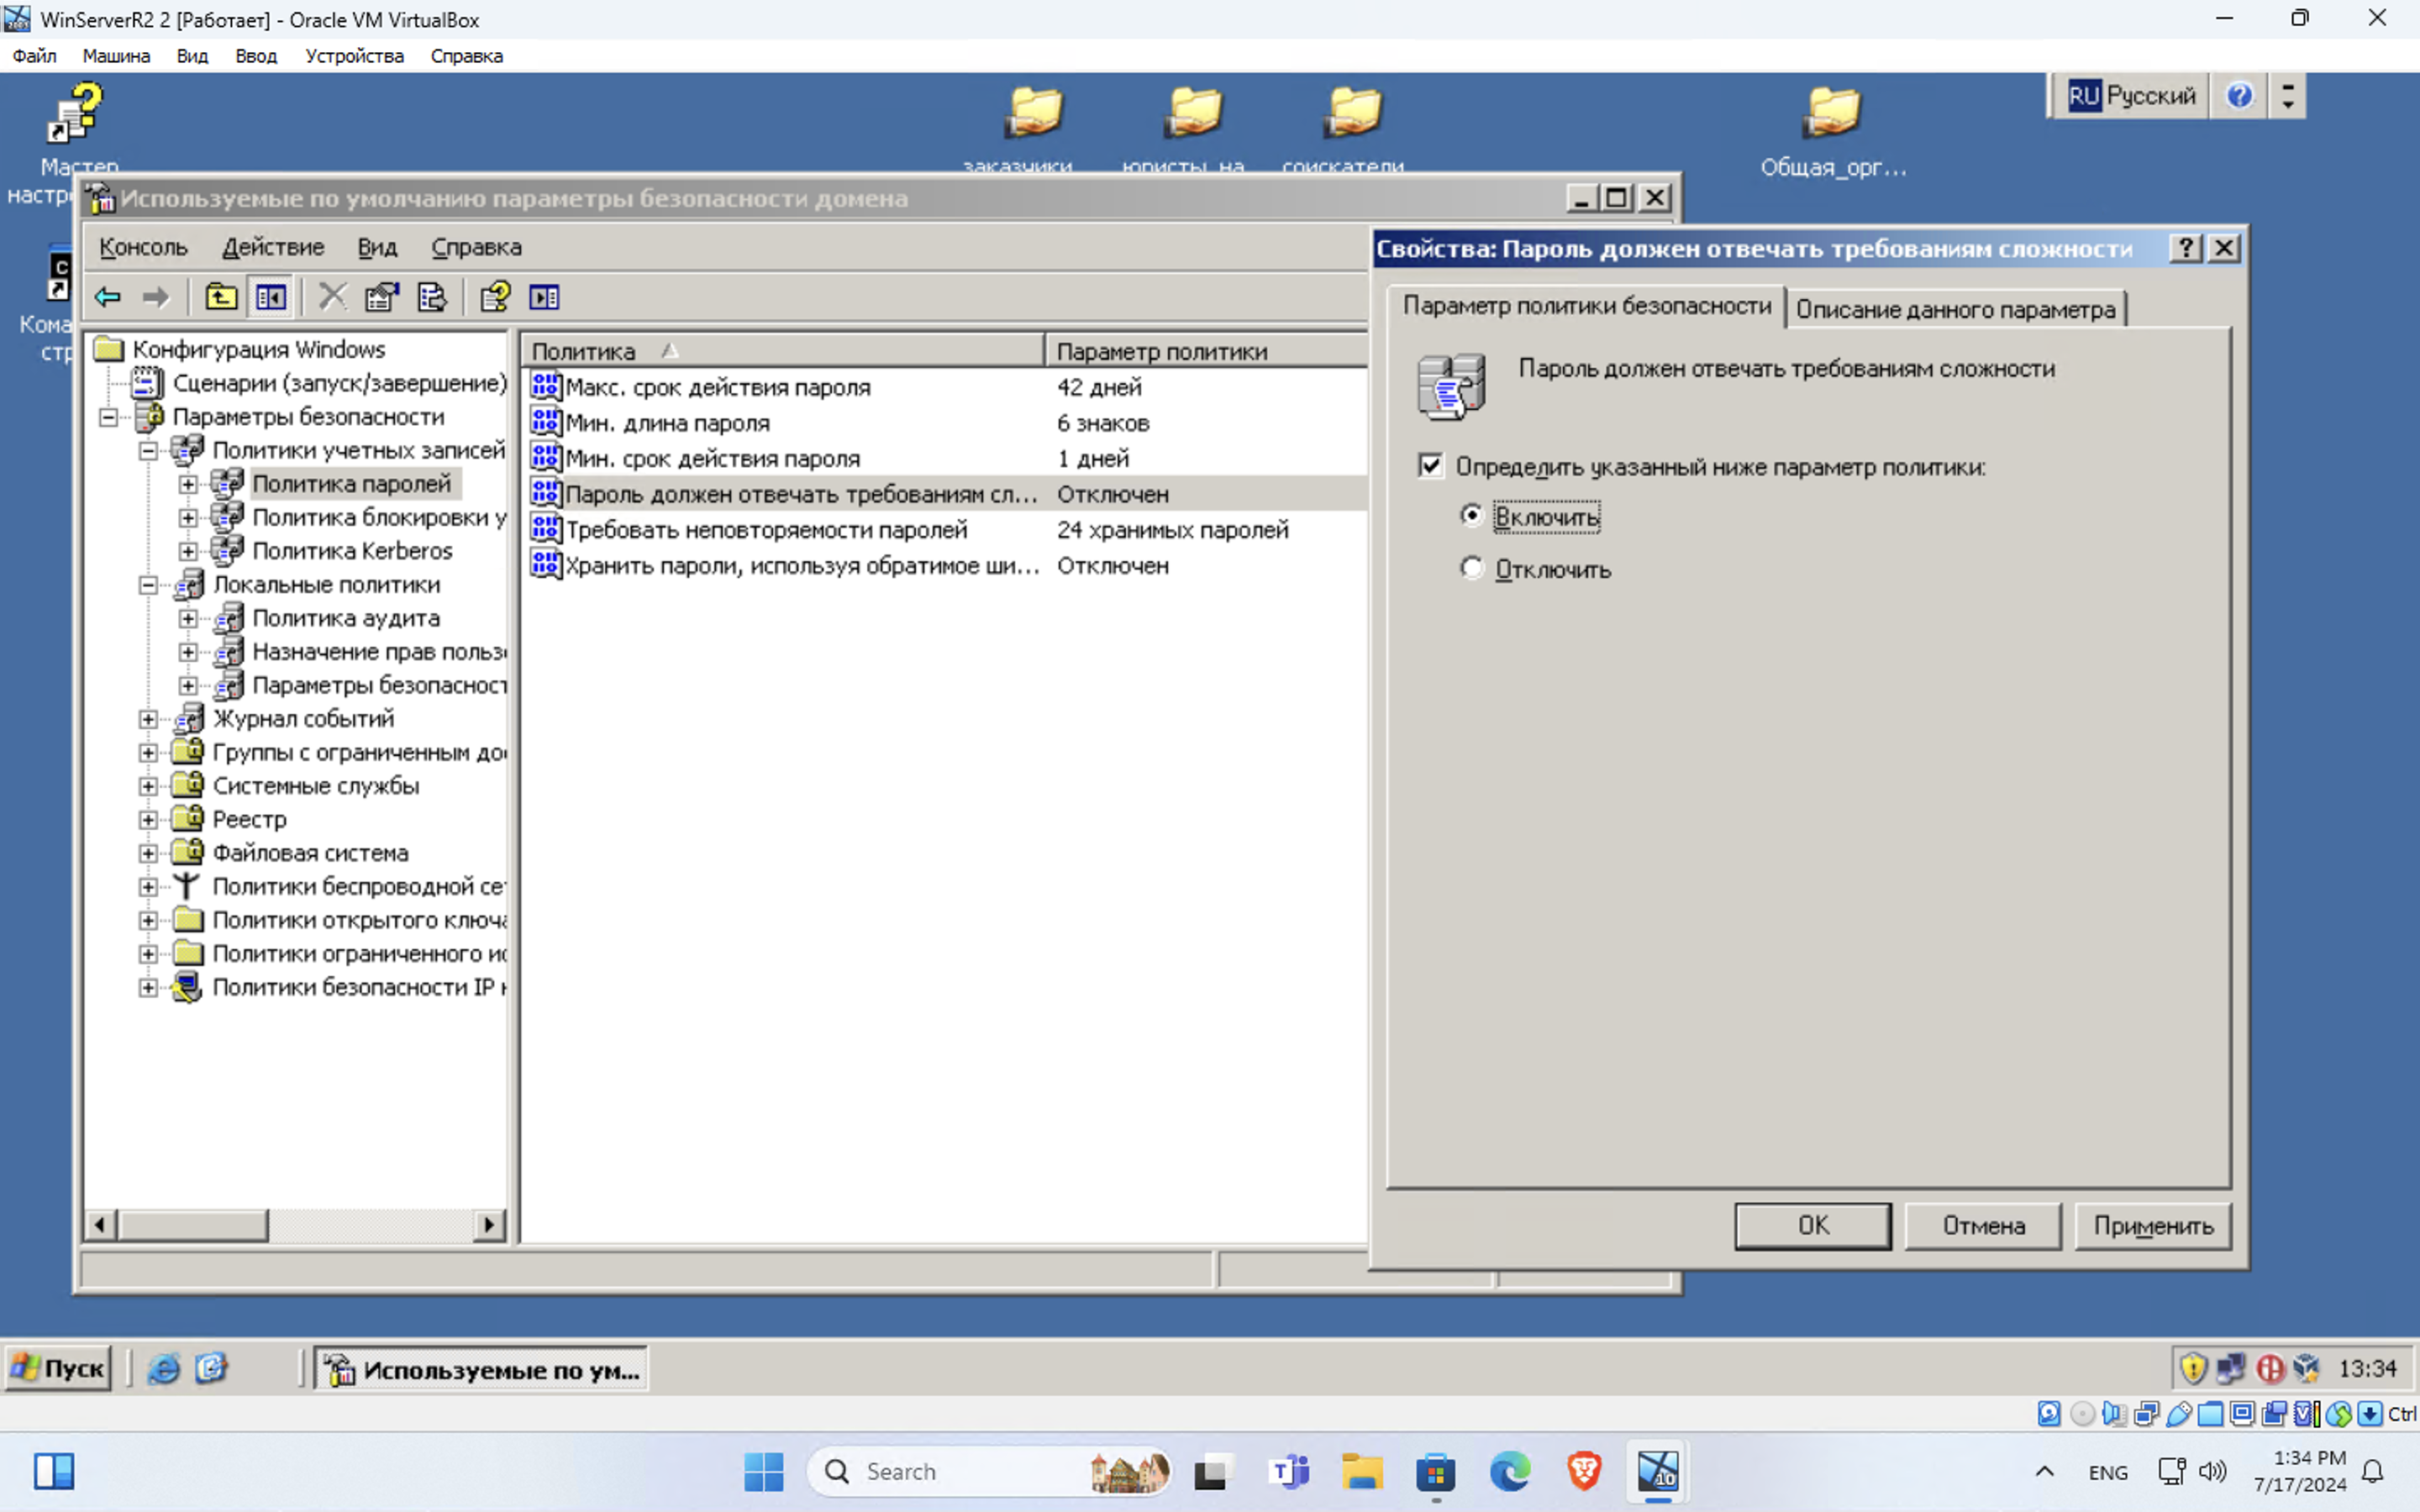
\includegraphics[width=1\textwidth]{pict/7}
  \caption{Парольная политика}
  \label{fig:19}
\end{figure}

Создадим пользователей в каждом подразделении.
\begin{figure}[H]
  \centering
  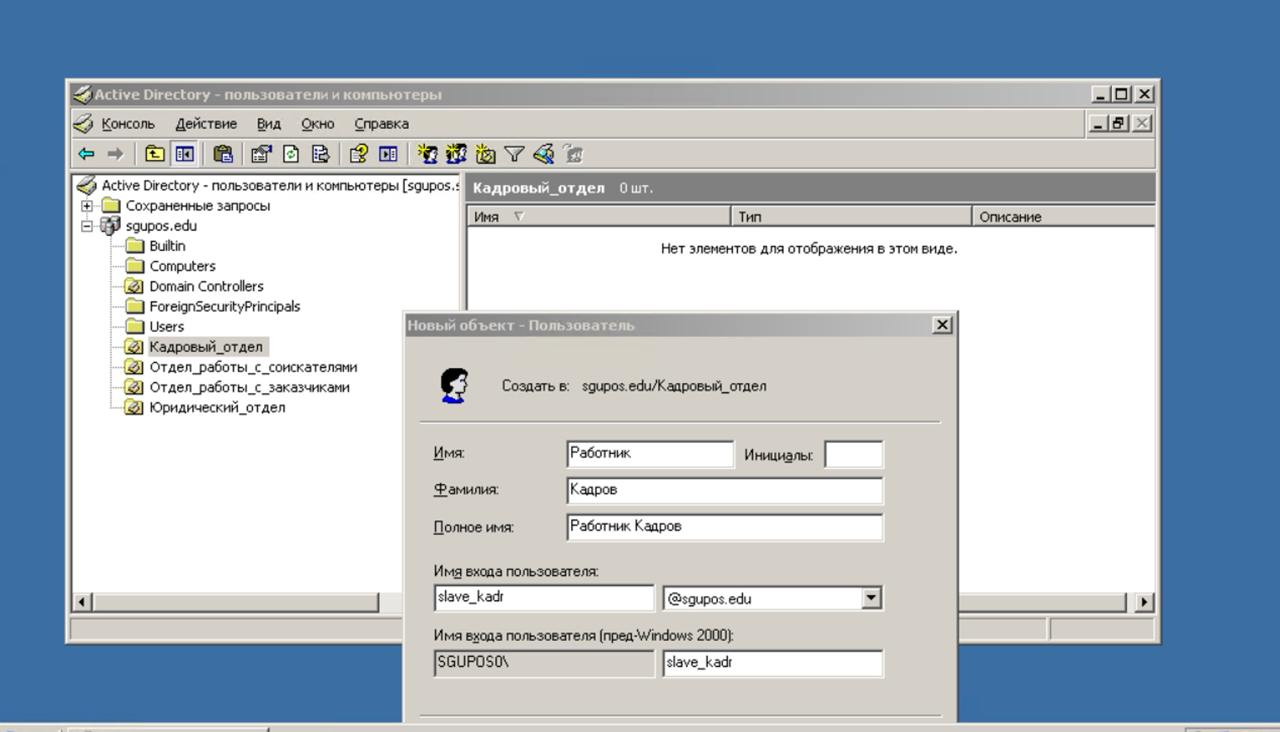
\includegraphics[width=1\textwidth]{pict/prac/1}
  \caption{Создание пользователя}
  \label{fig:12}
\end{figure}

\begin{figure}[H]
  \centering
  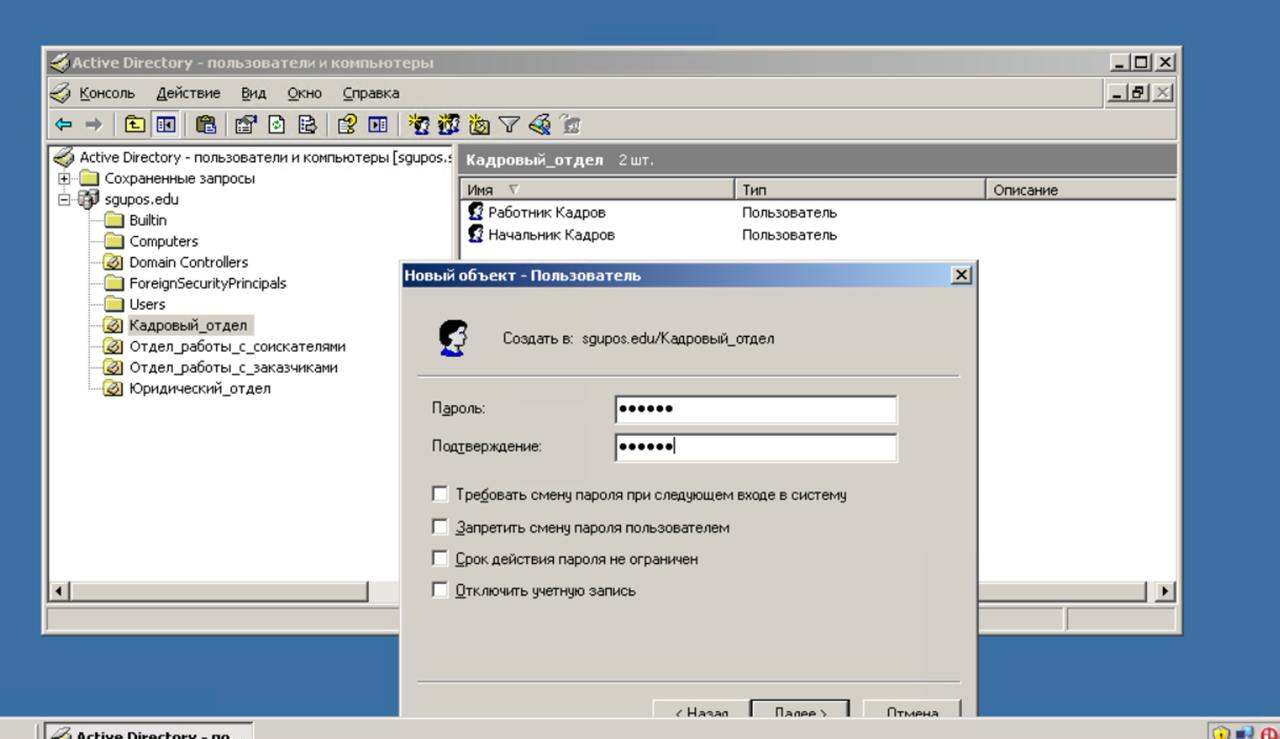
\includegraphics[width=1\textwidth]{pict/prac/2}
  \caption{Задание пароля пользователю}
  \label{fig:14}
\end{figure}

Проверим работу настройки сложности пароля, поменяем пользователю пароль.
\begin{figure}[H]
  \centering
  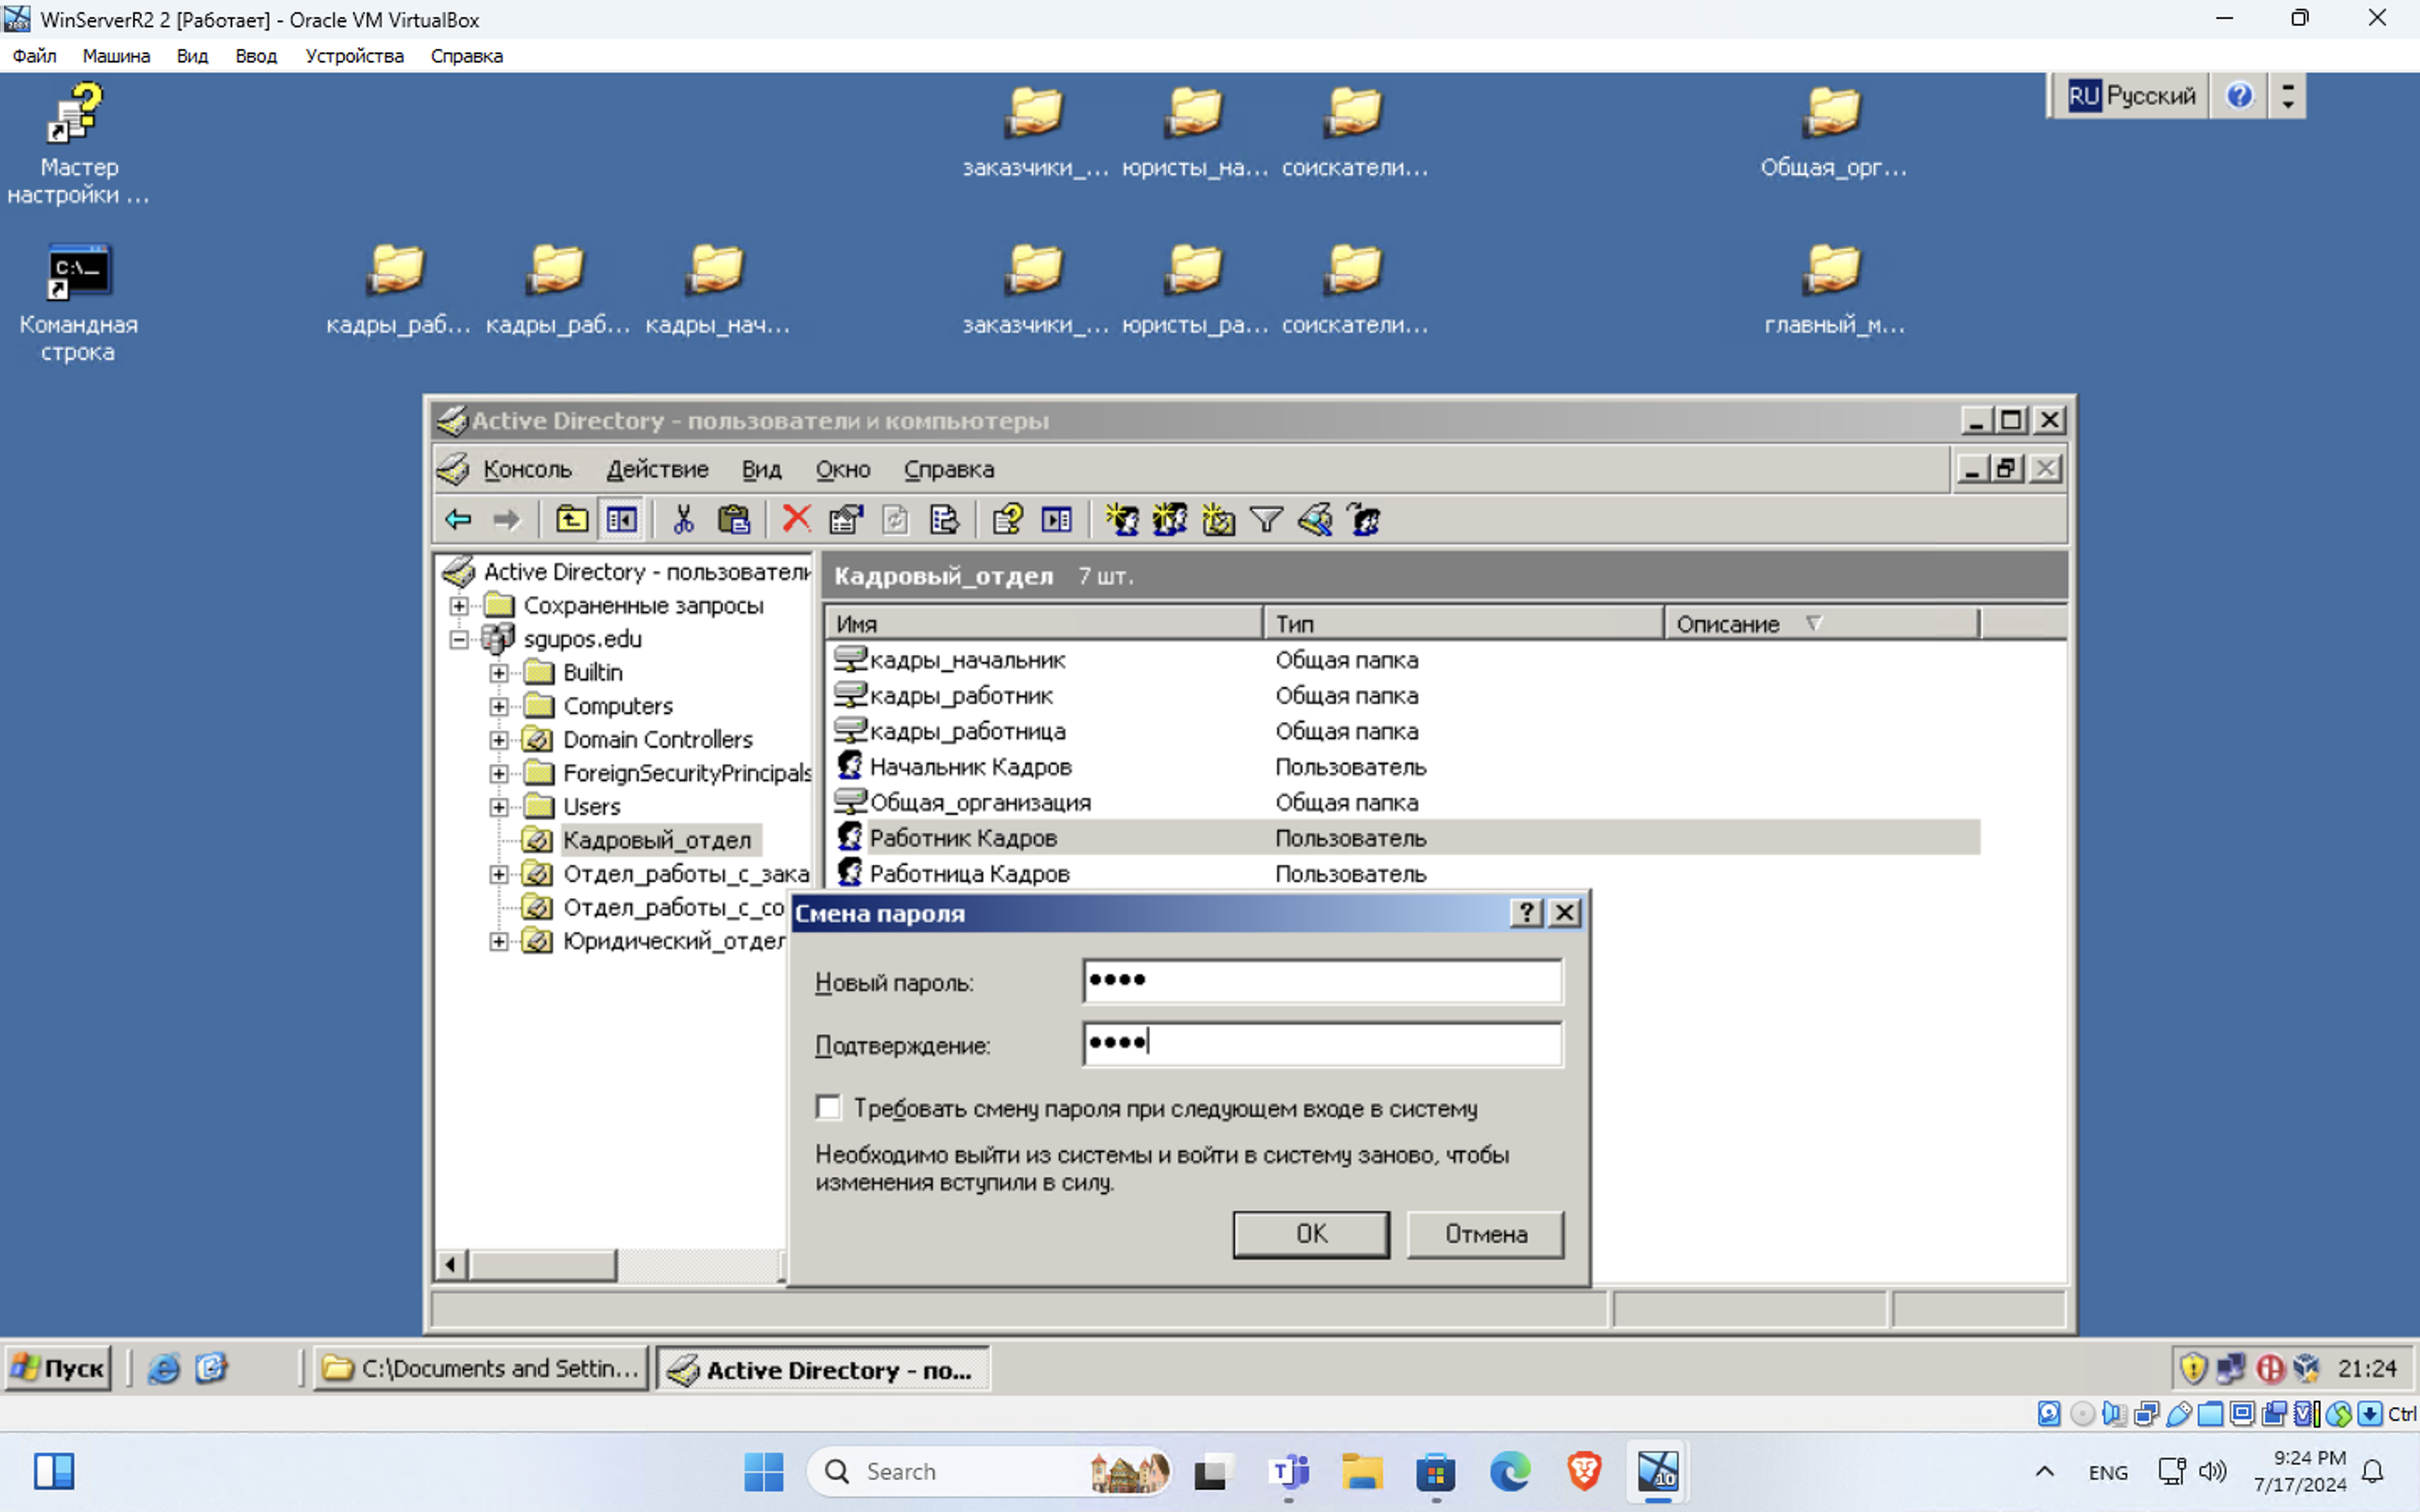
\includegraphics[width=1\textwidth]{pict/prac/50}
  \caption{Поменяем пароль на более короткий}
  \label{fig:50}
\end{figure}

\begin{figure}[H]
  \centering
  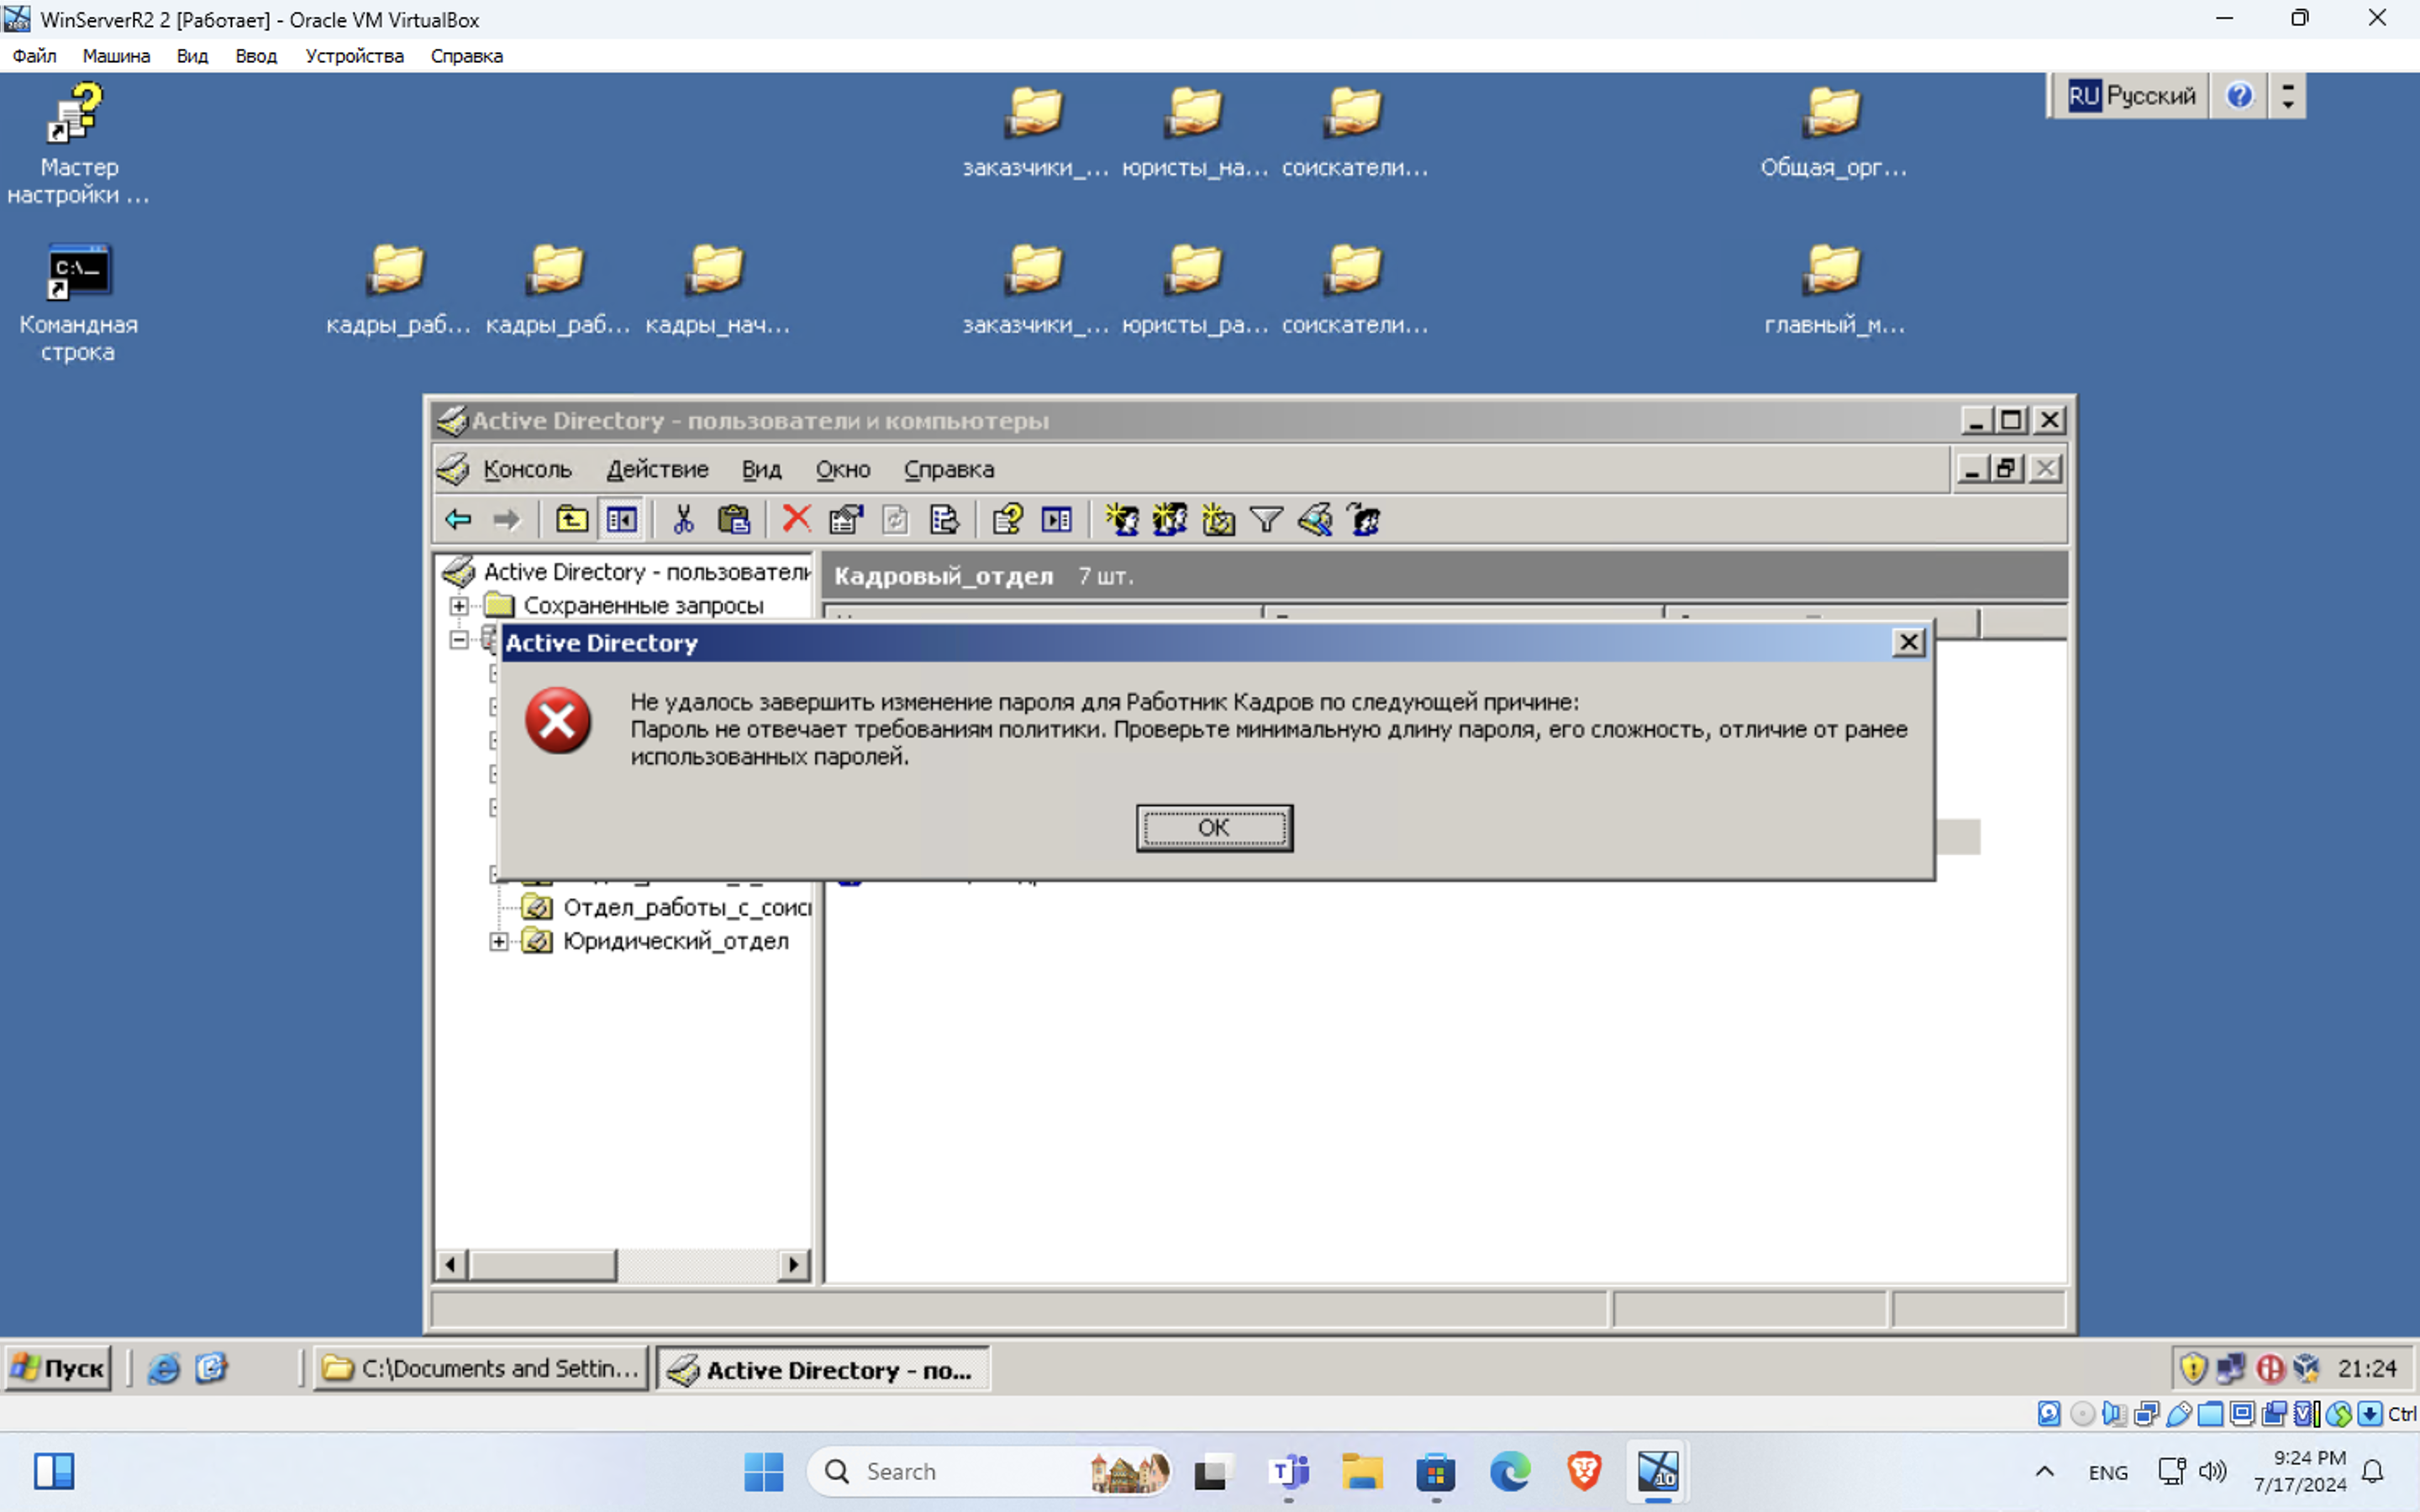
\includegraphics[width=0.9\textwidth]{pict/prac/51}
  \caption{Реакция системы на смену пароля}
  \label{fig:51}
\end{figure}

Создадим настройку ограниченного доступа к журналу, соответствующую требованию к уровню защищенности ИС.
\begin{figure}[H]
  \centering
  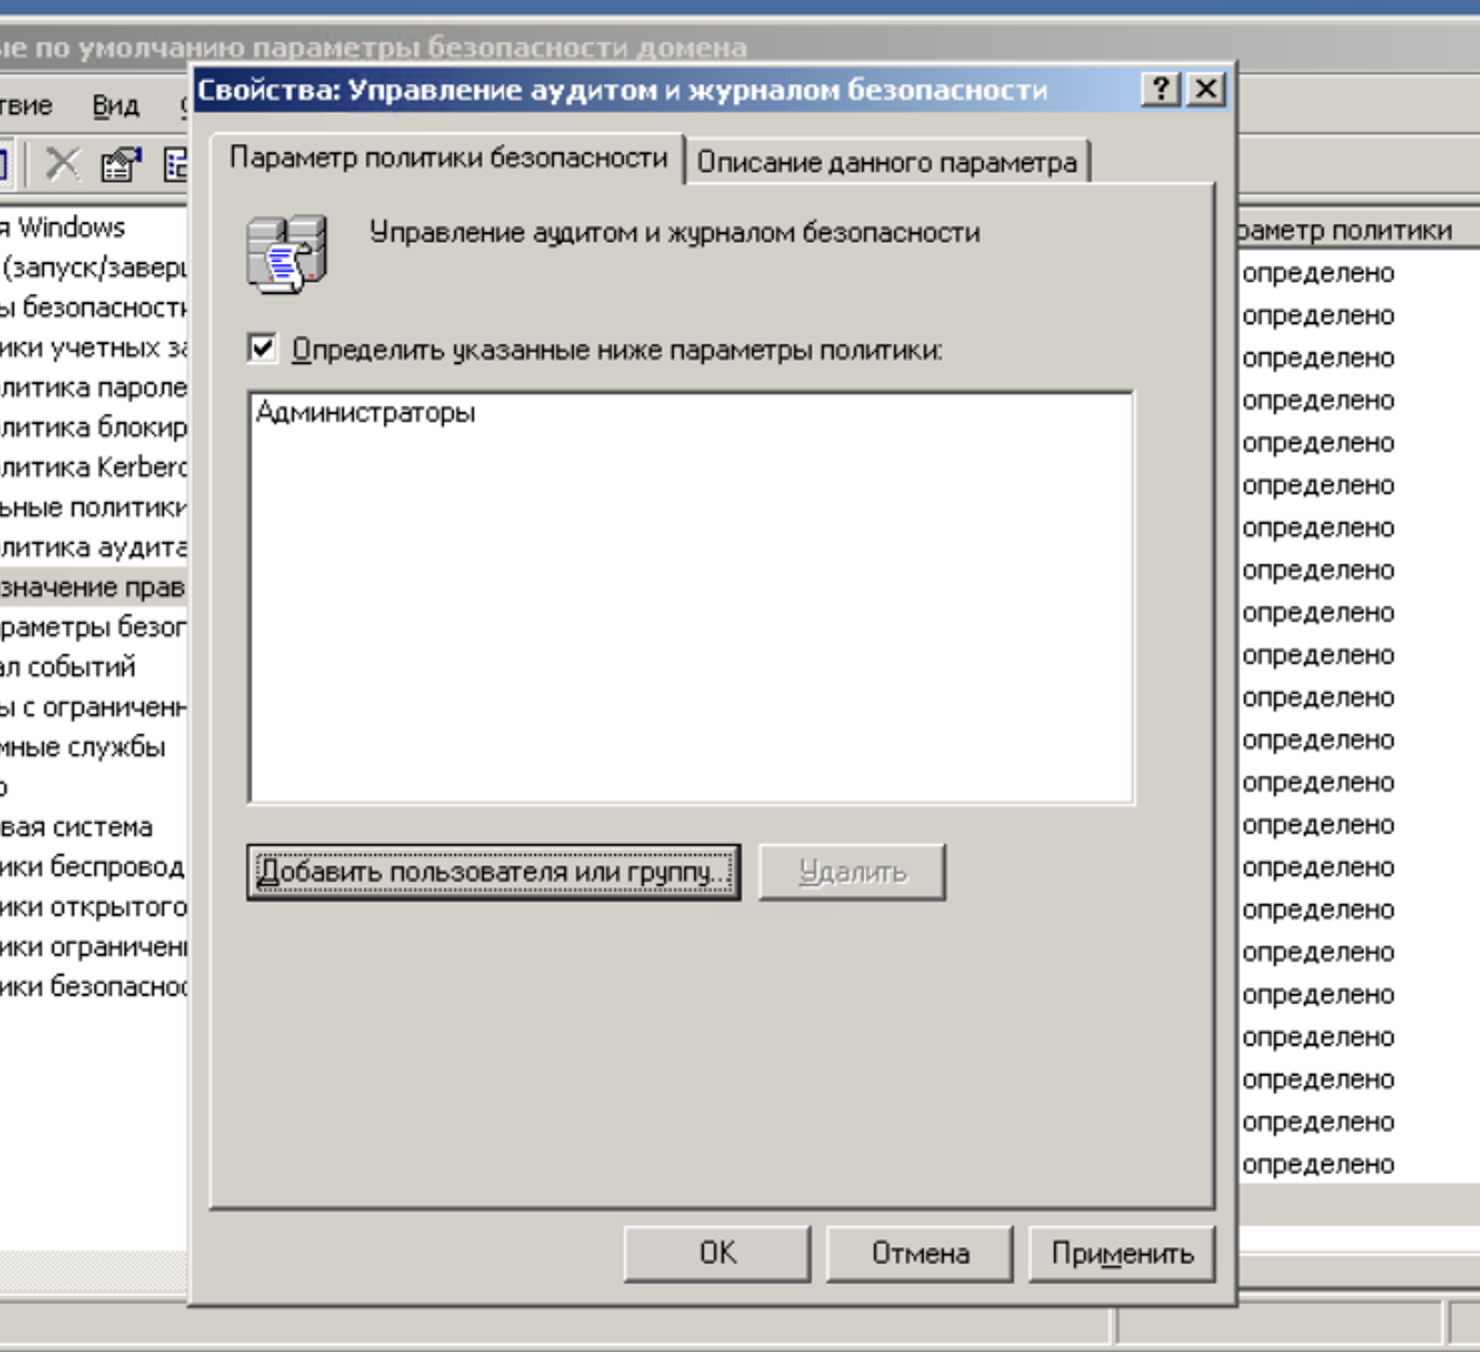
\includegraphics[width=1\textwidth]{pict/prac/59}
  \caption{Ограничение доступа к журналу}
\end{figure}

Зайдем в аккаунт одного оз пользователей и попробуем посмотреть журнал безопасность.
\begin{figure}[H]
  \centering
  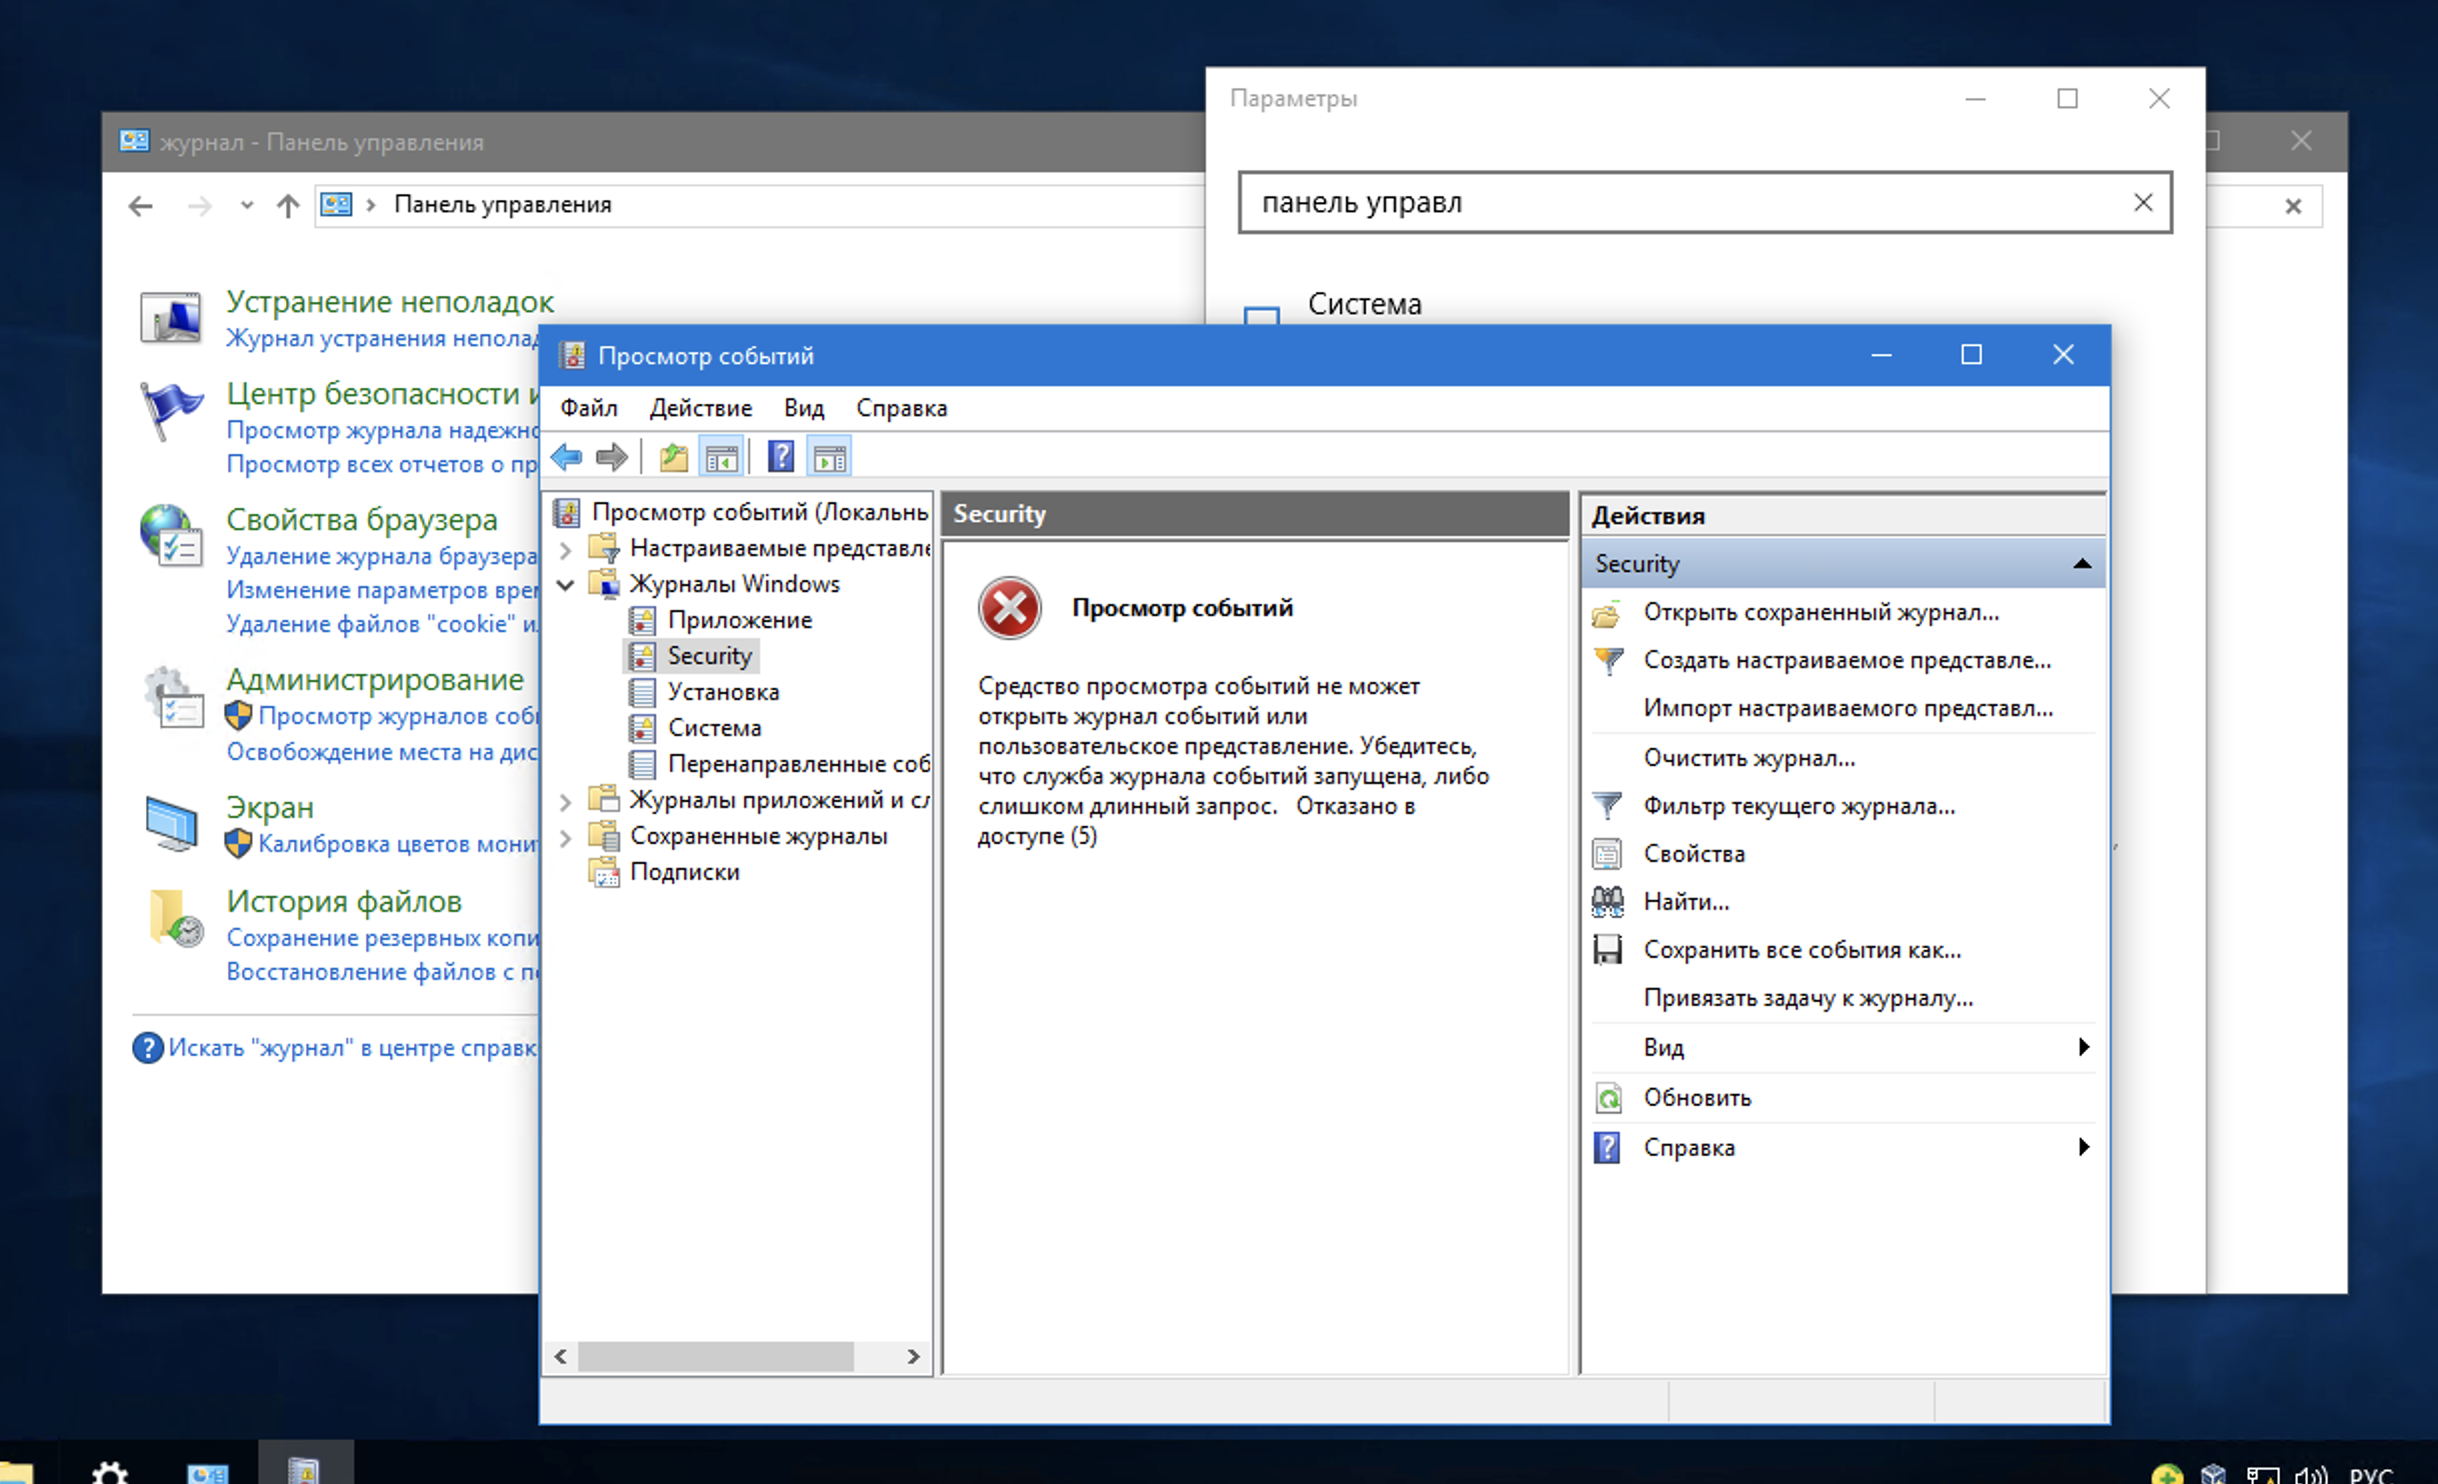
\includegraphics[width=1\textwidth]{pict/prac/80}
  \caption{Реакция на доступ к журналу}
\end{figure}

Также чтобы в систему имели доступ только аутентифицированные пользователи, отключим учетную запись гостя.

\begin{figure}[H]
  \centering
  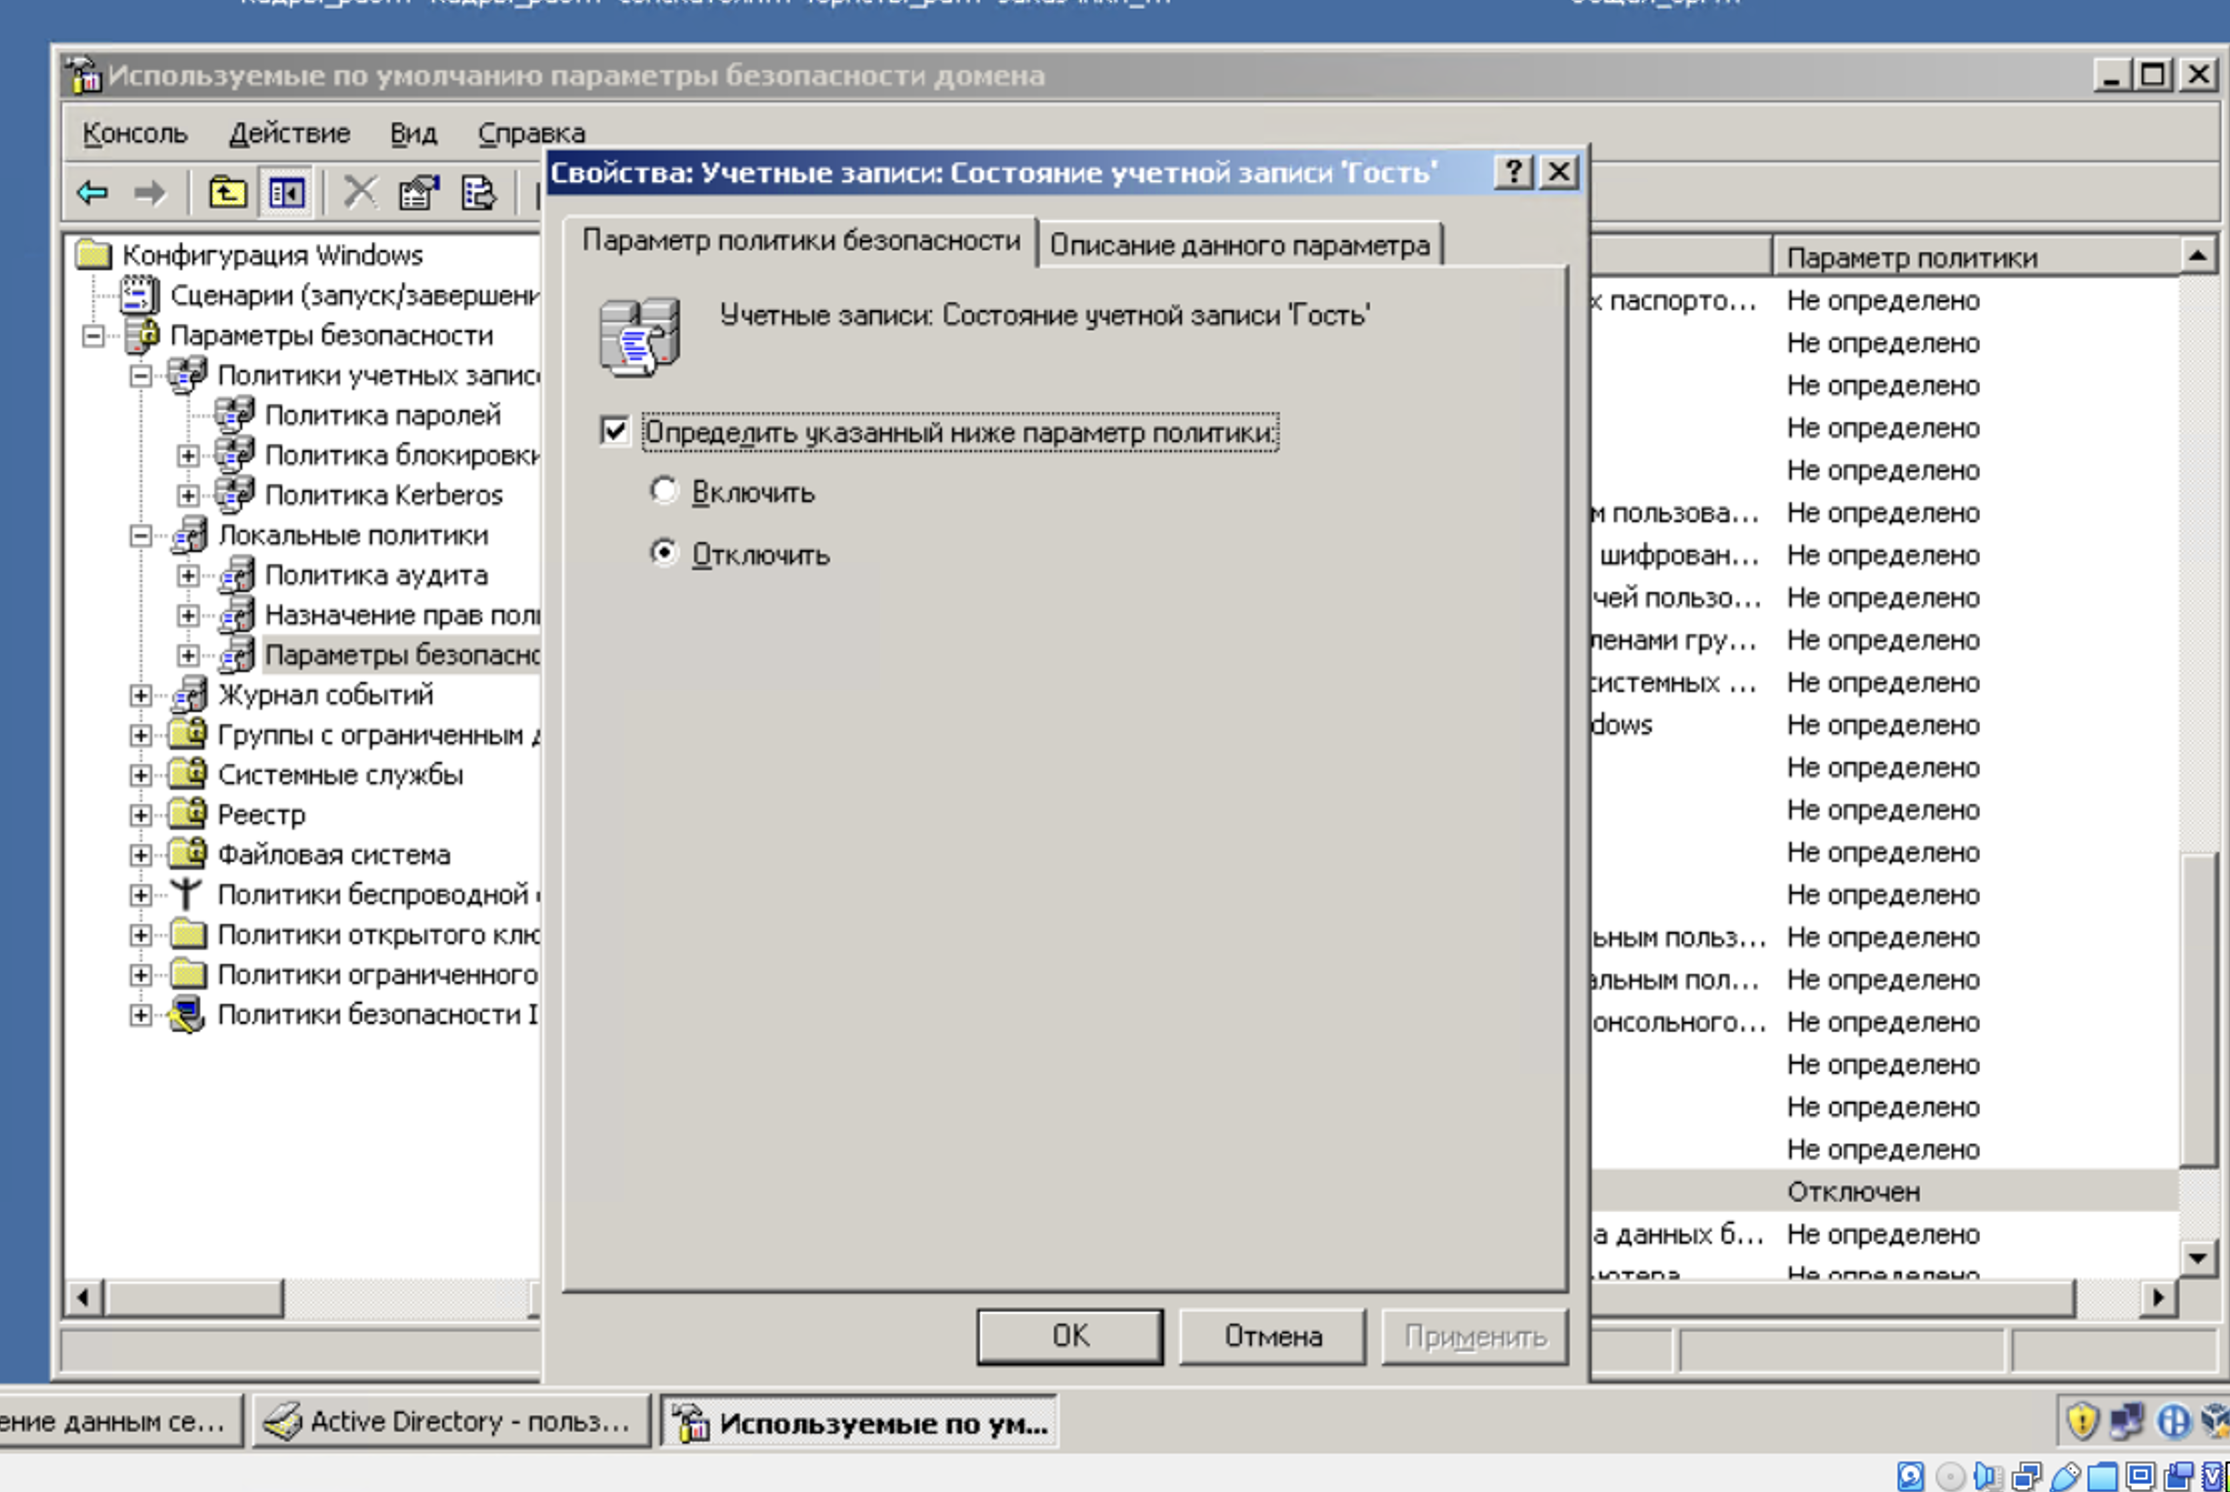
\includegraphics[width=1\textwidth]{pict/prac/60}
  \caption{Запрет гостевой учетной записи}
\end{figure}

Проверим работ предыдущей политики.
\begin{figure}[H]
  \centering
  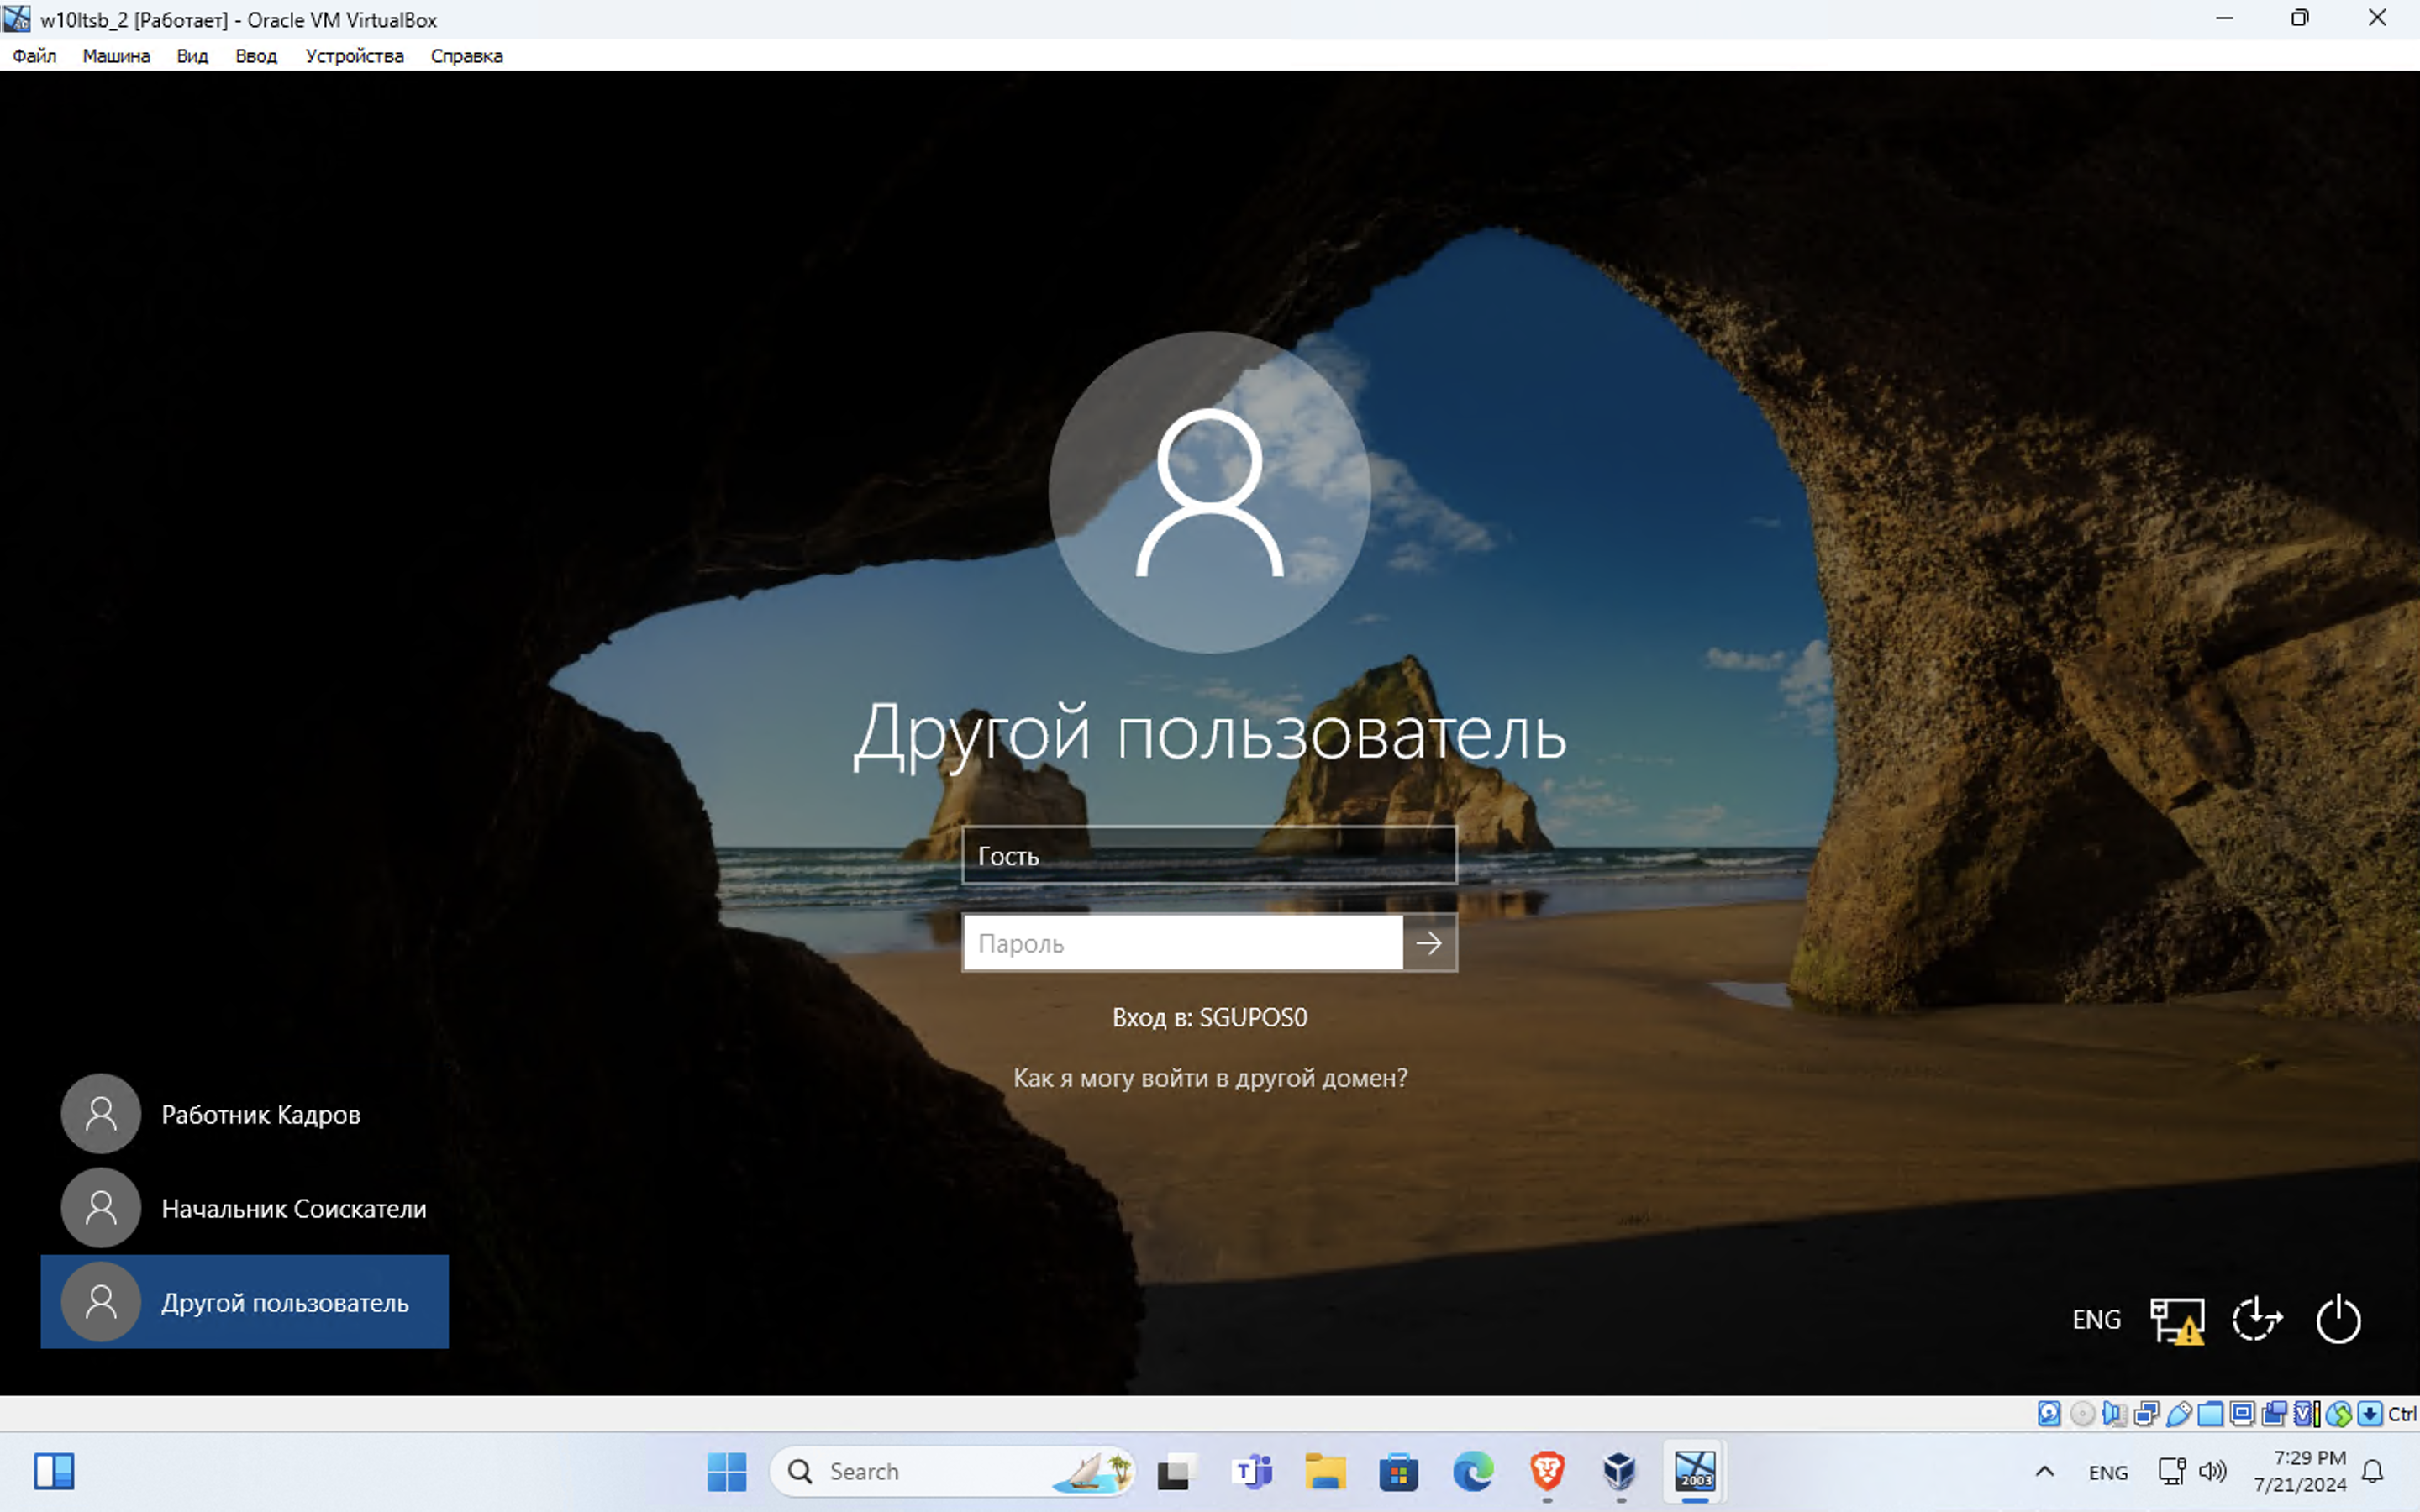
\includegraphics[width=1\textwidth]{pict/prac/65}
  \caption{Реакция системы на вход гостя}
\end{figure}

\begin{figure}[H]
  \centering
  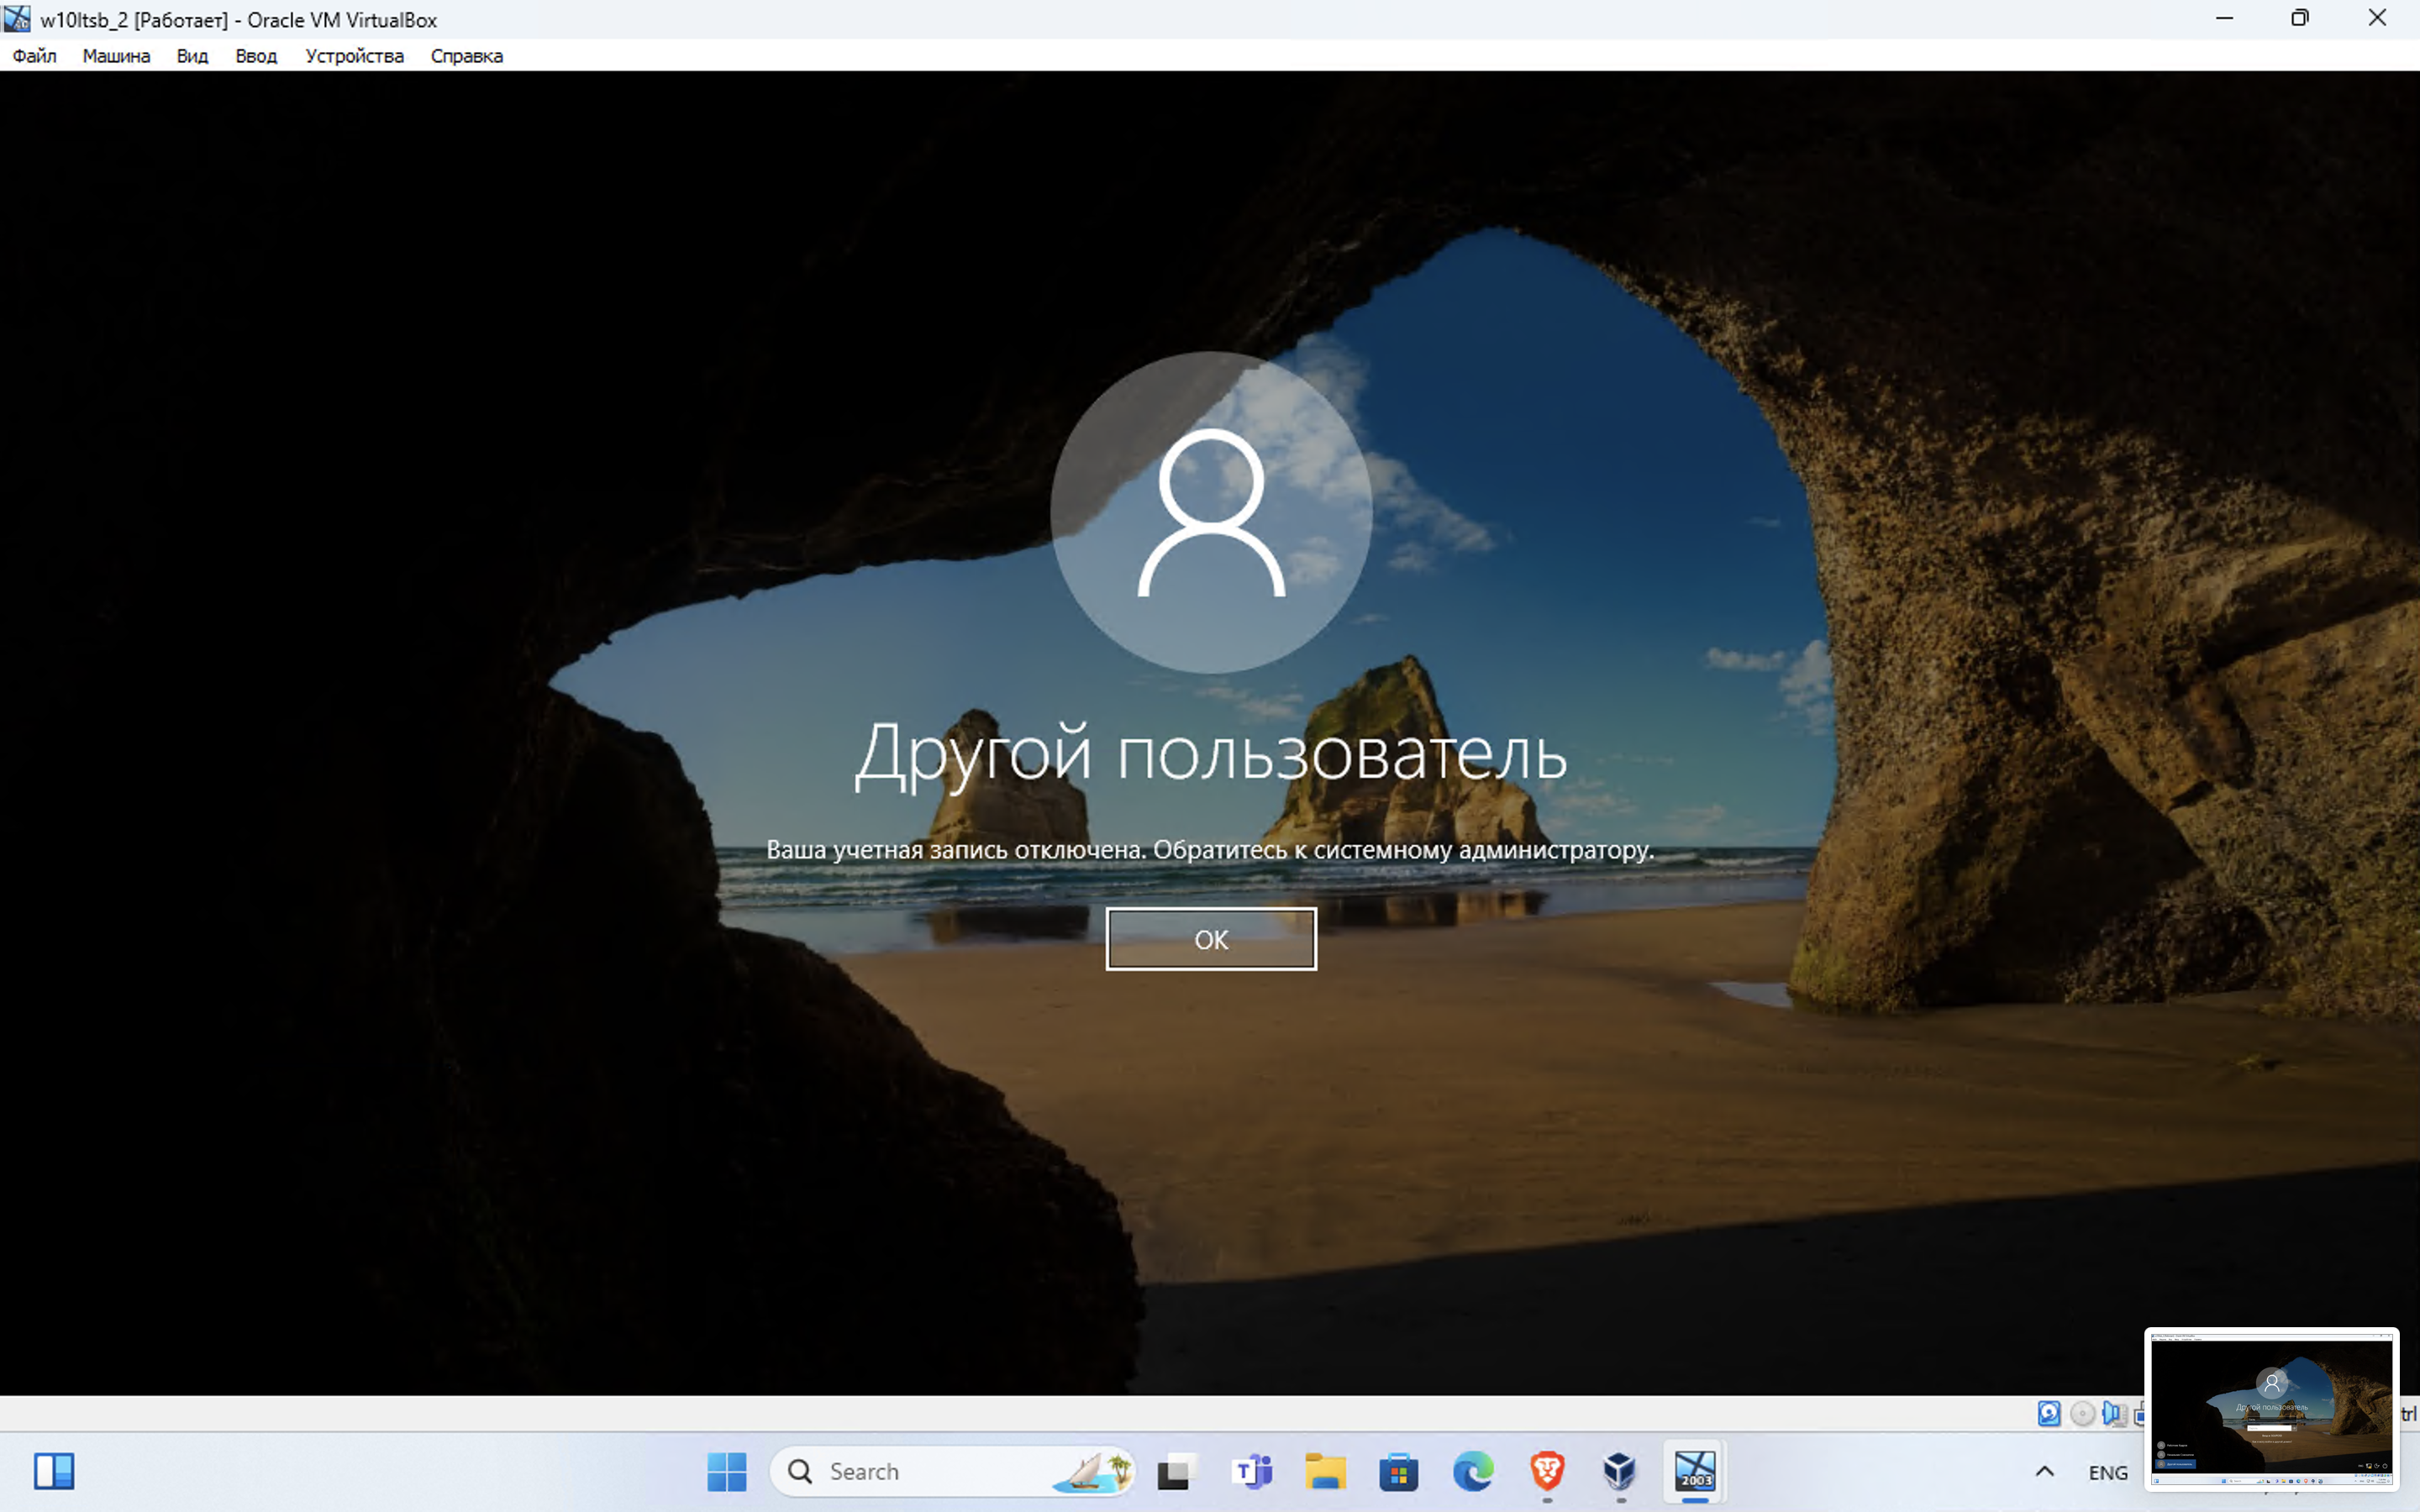
\includegraphics[width=1\textwidth]{pict/prac/66}
  \caption{Реакция системы на вход гостя}
\end{figure}

Аналогично создадим всех остальных пользователей для каждого подразделения.

\begin{figure}[H]
  \centering
  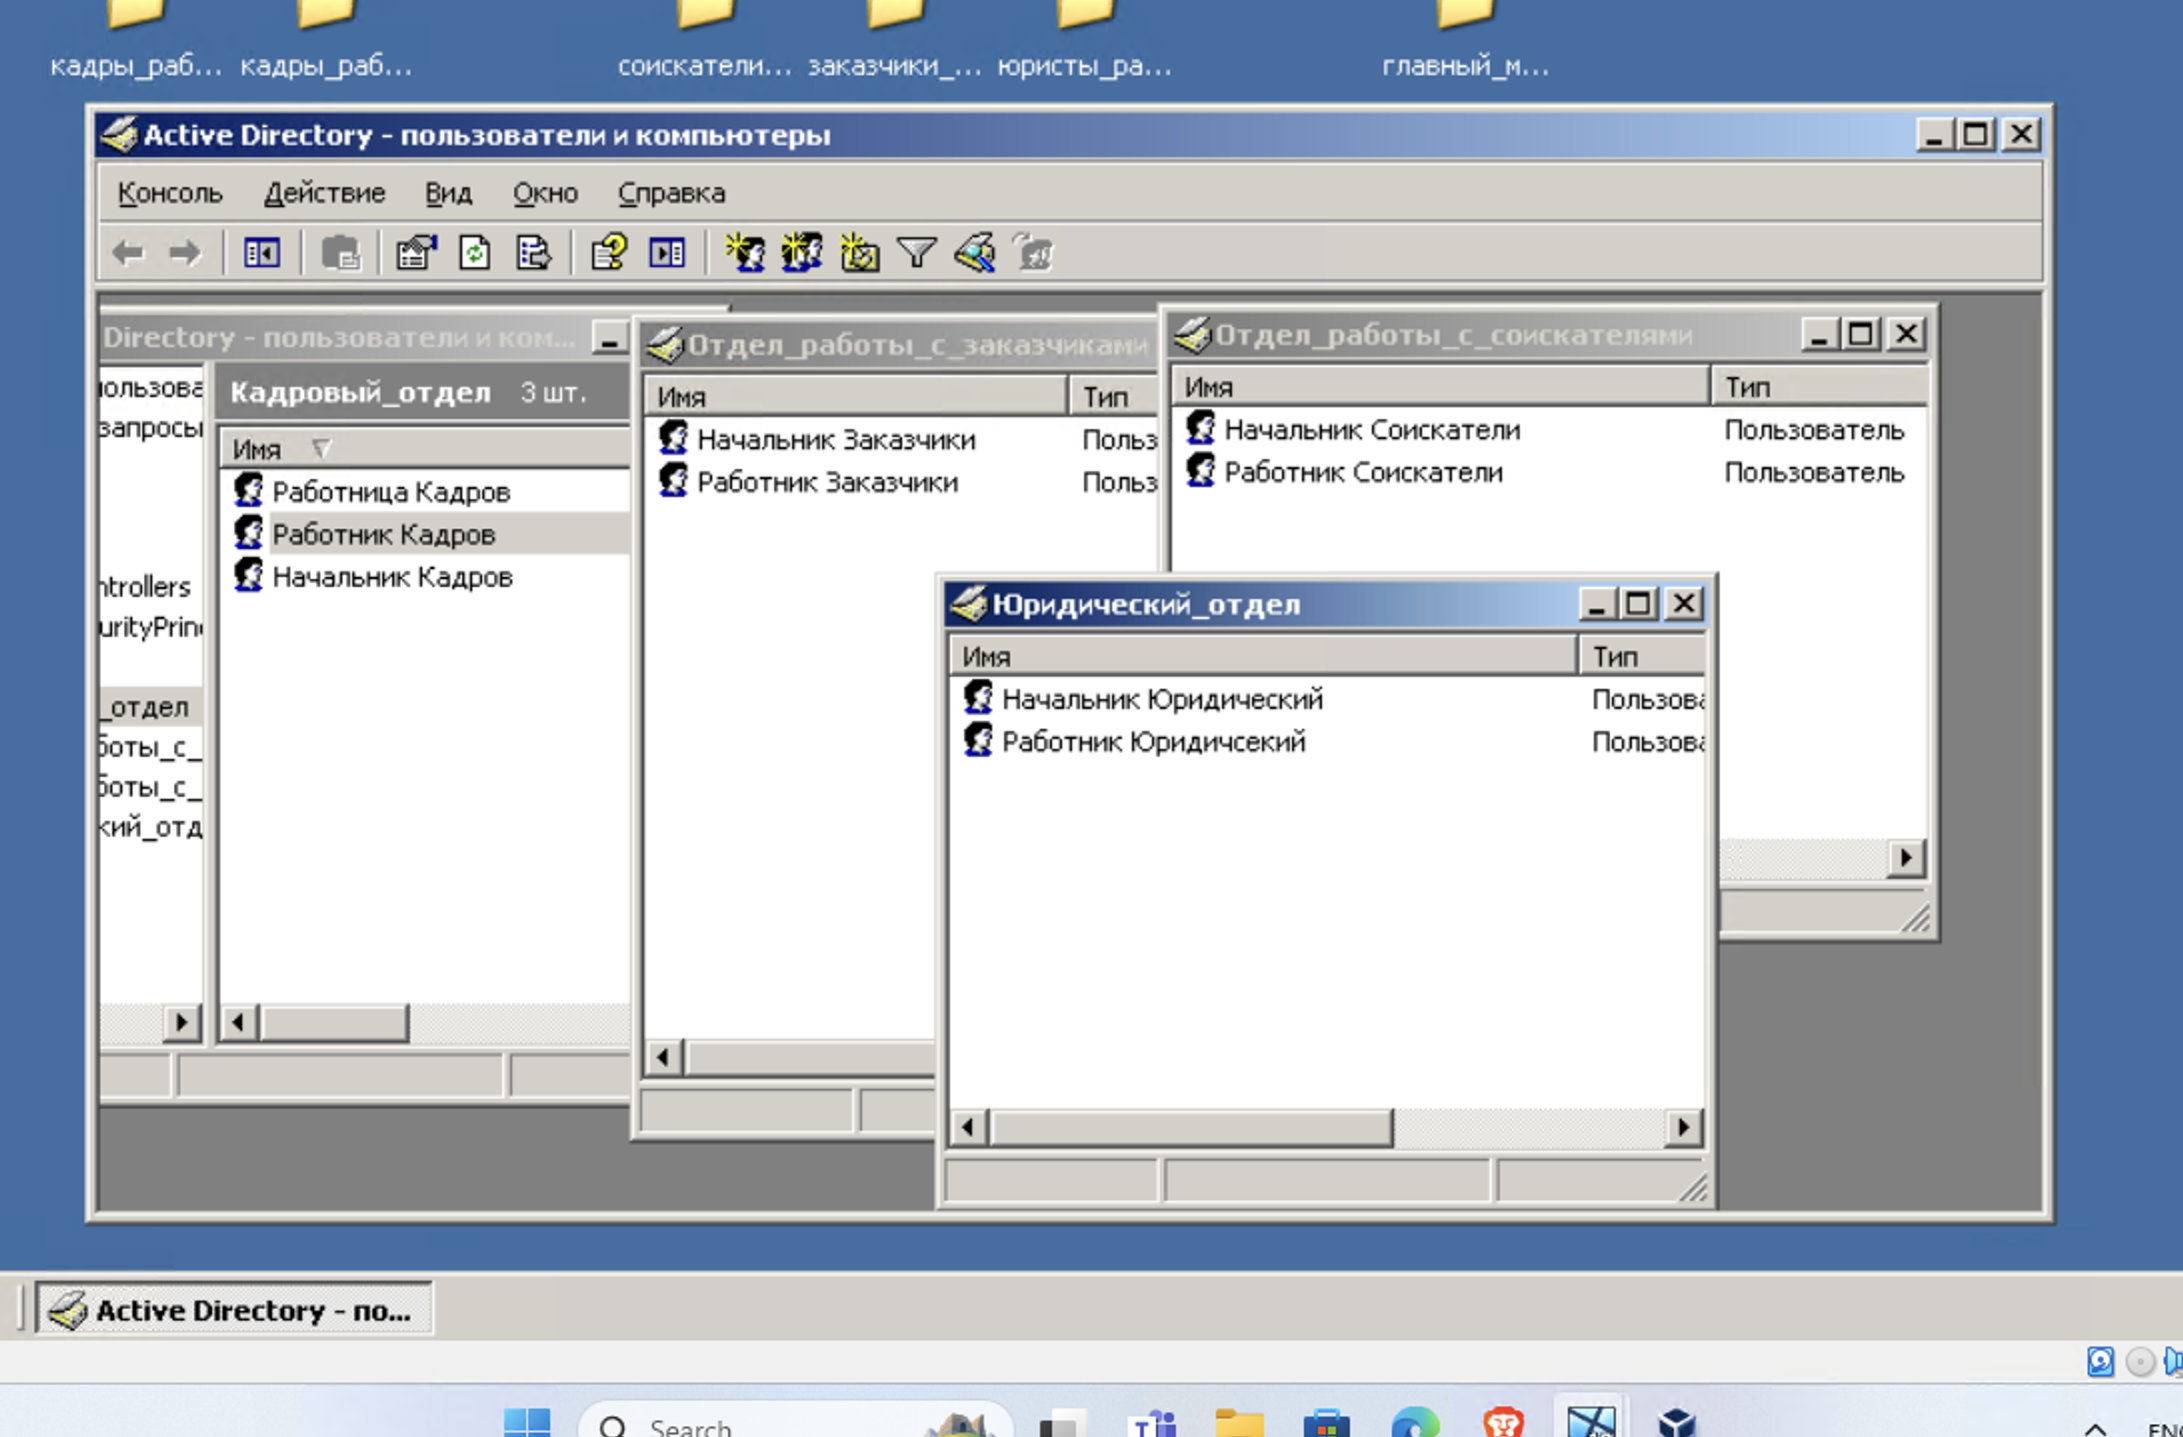
\includegraphics[width=0.9\textwidth]{pict/prac/4}
  \caption{Аккаунты работников}
  \label{fig:15}
\end{figure}

Создадим сетевой ресурс для общей папки во всех отделах, так как папка нужна для обмена данными, то 
все имеют право туда писать, читать, но изменять содержимое чужих файлов нет.

\begin{figure}[H]
  \centering
  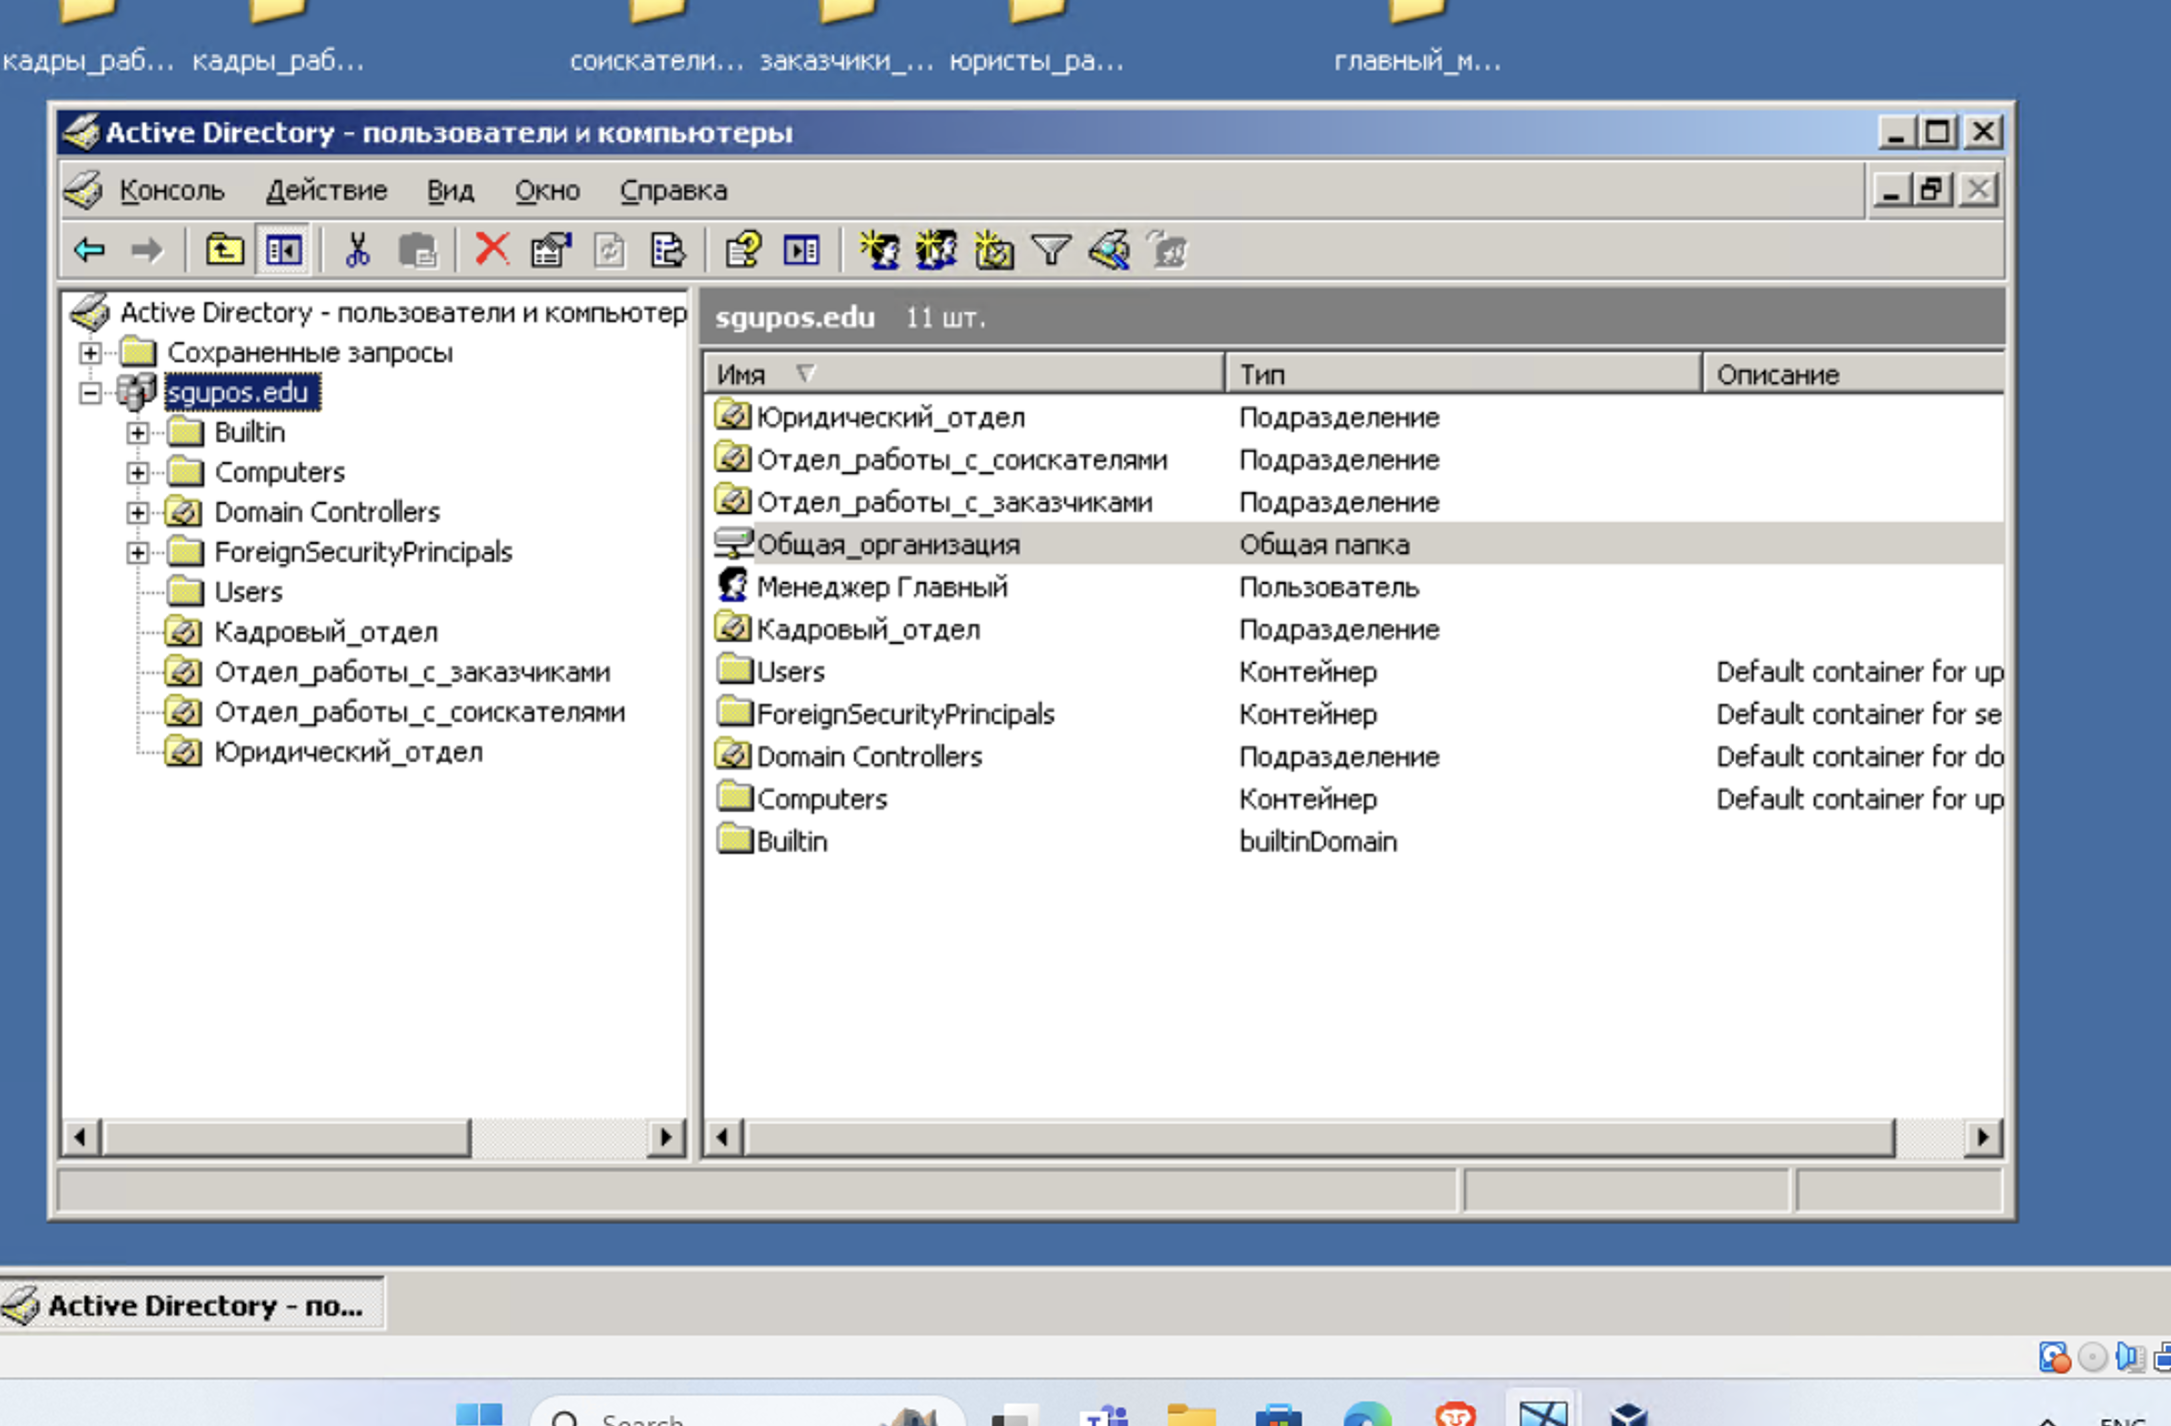
\includegraphics[width=0.9\textwidth]{pict/prac/5}
  \caption{Общая папка}
  \label{fig:16}
\end{figure}

\begin{figure}[H]
  \centering
  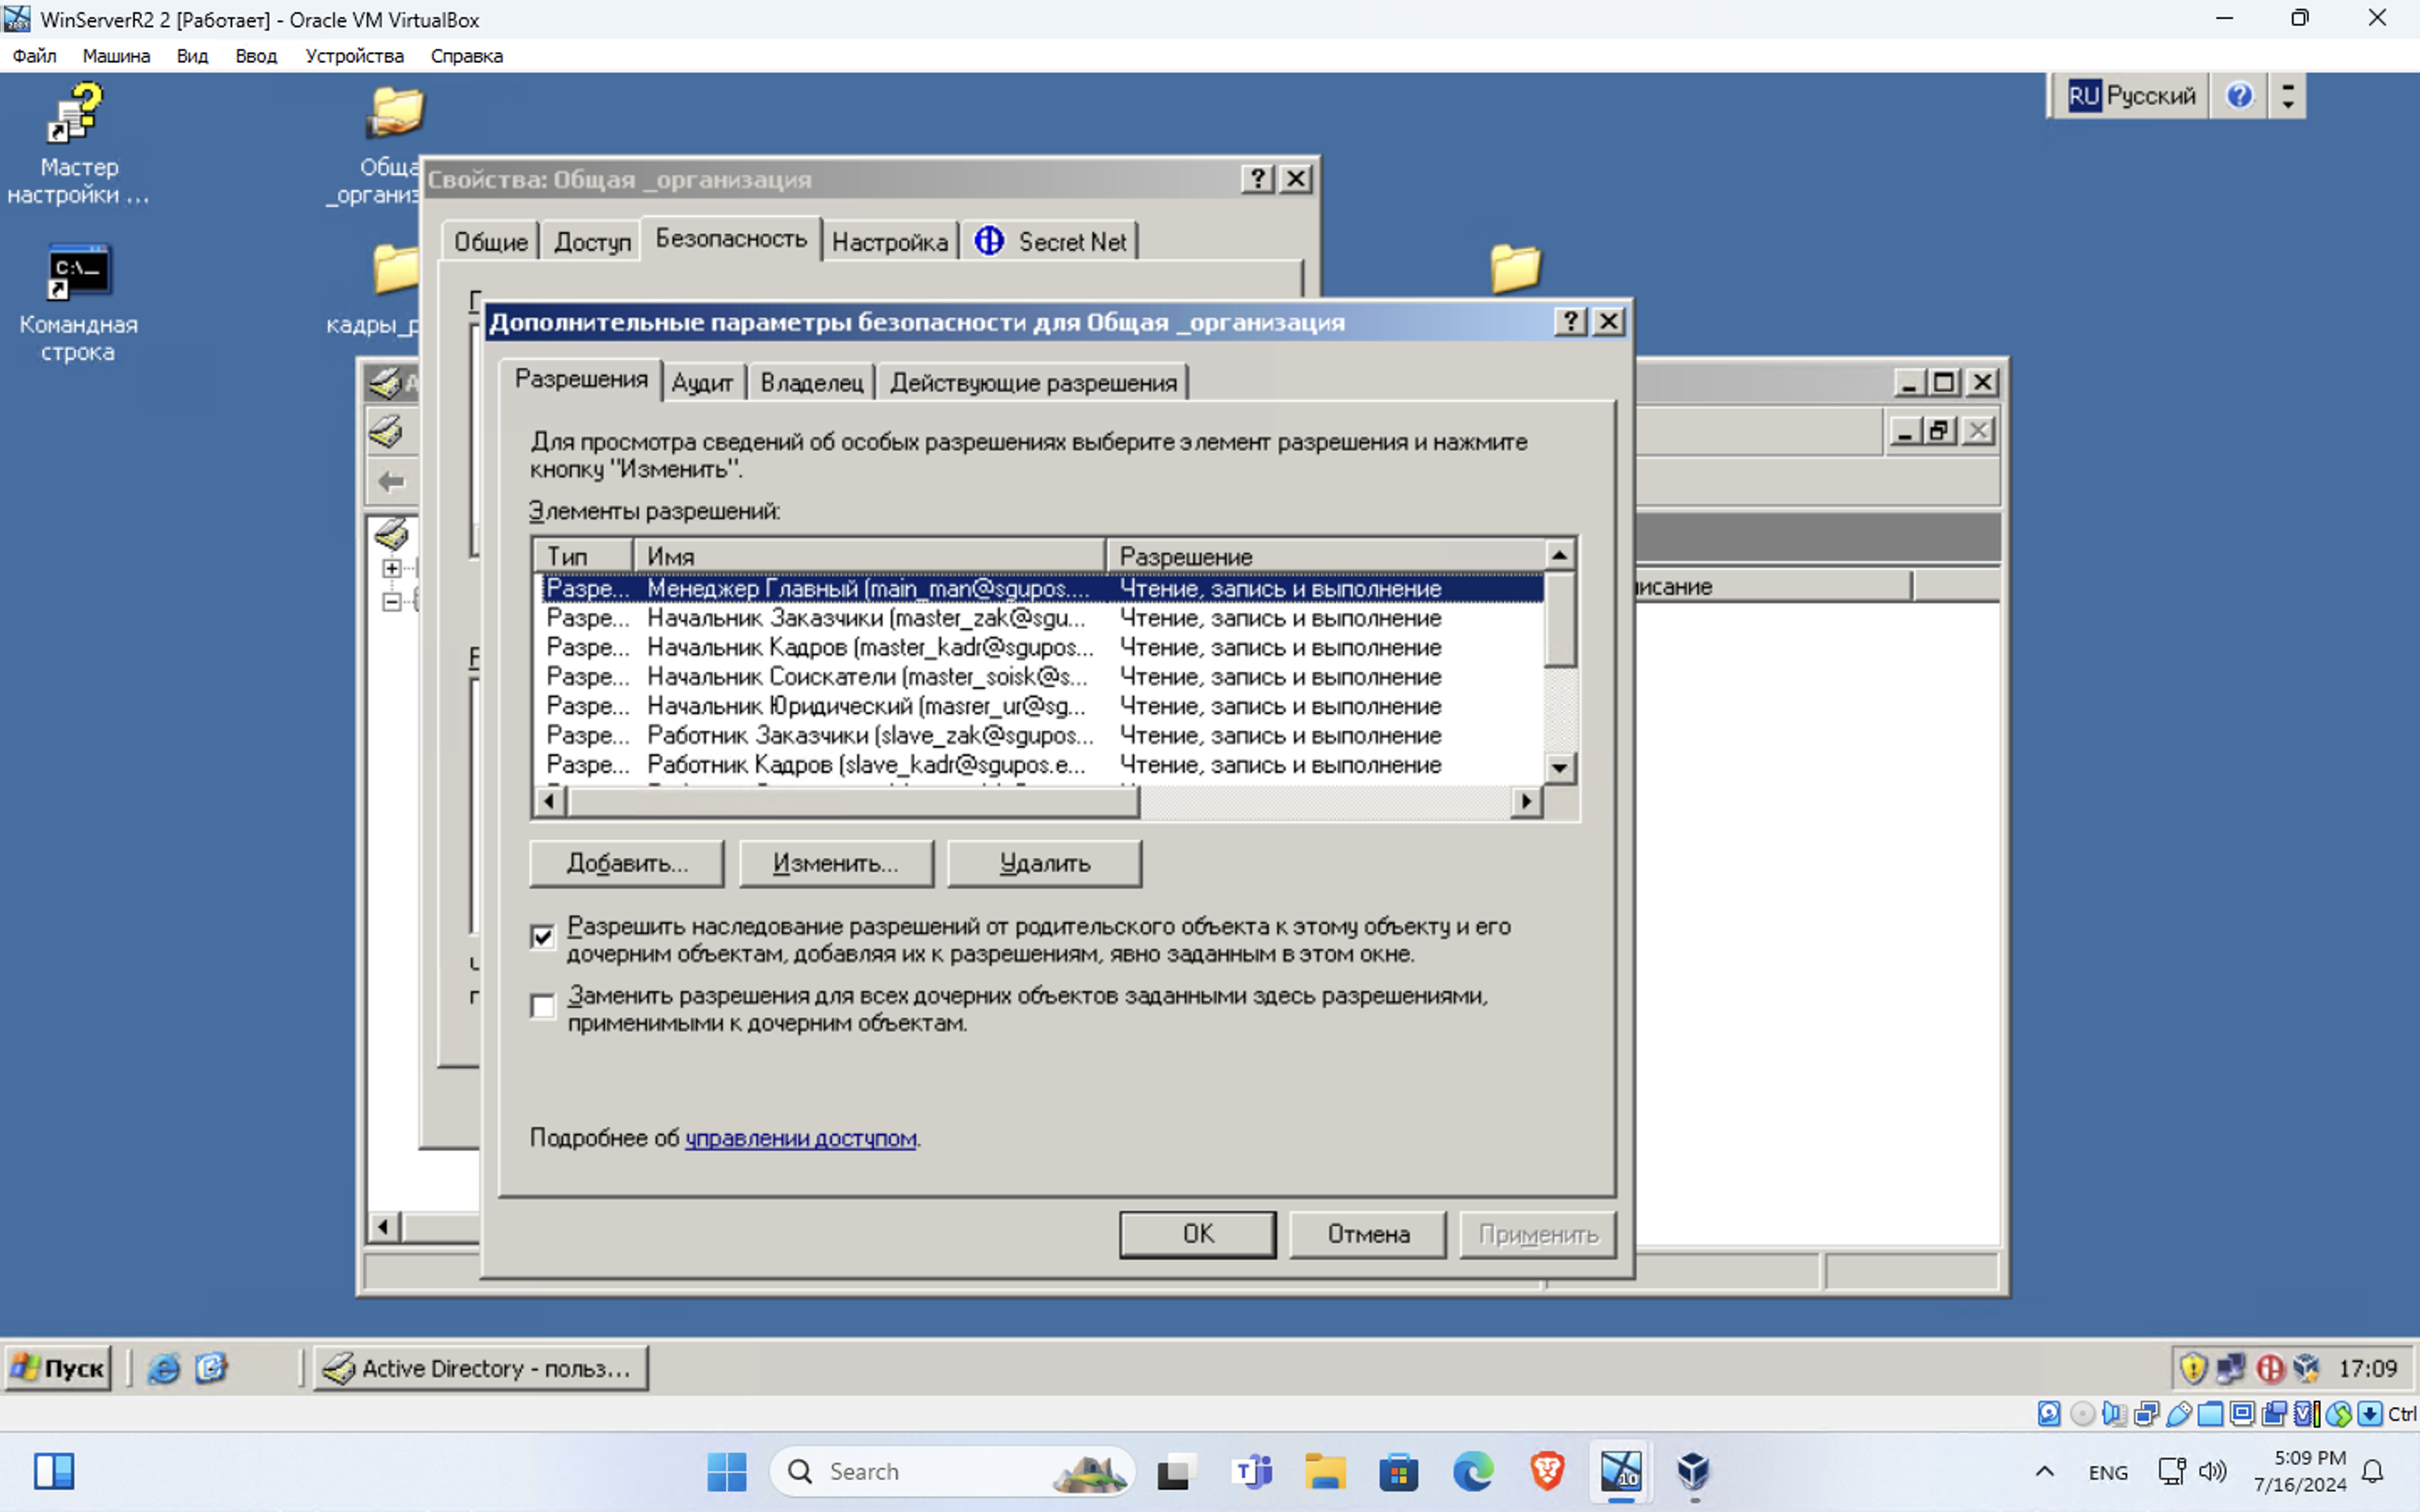
\includegraphics[width=0.9\textwidth]{pict/prac/6}
  \caption{Права на общую папку}
  \label{fig:17}
\end{figure}


Также создадим в каждом подразделении будет сетевой ресурс, указывающий на общую папку.
\begin{figure}[H]
  \centering
  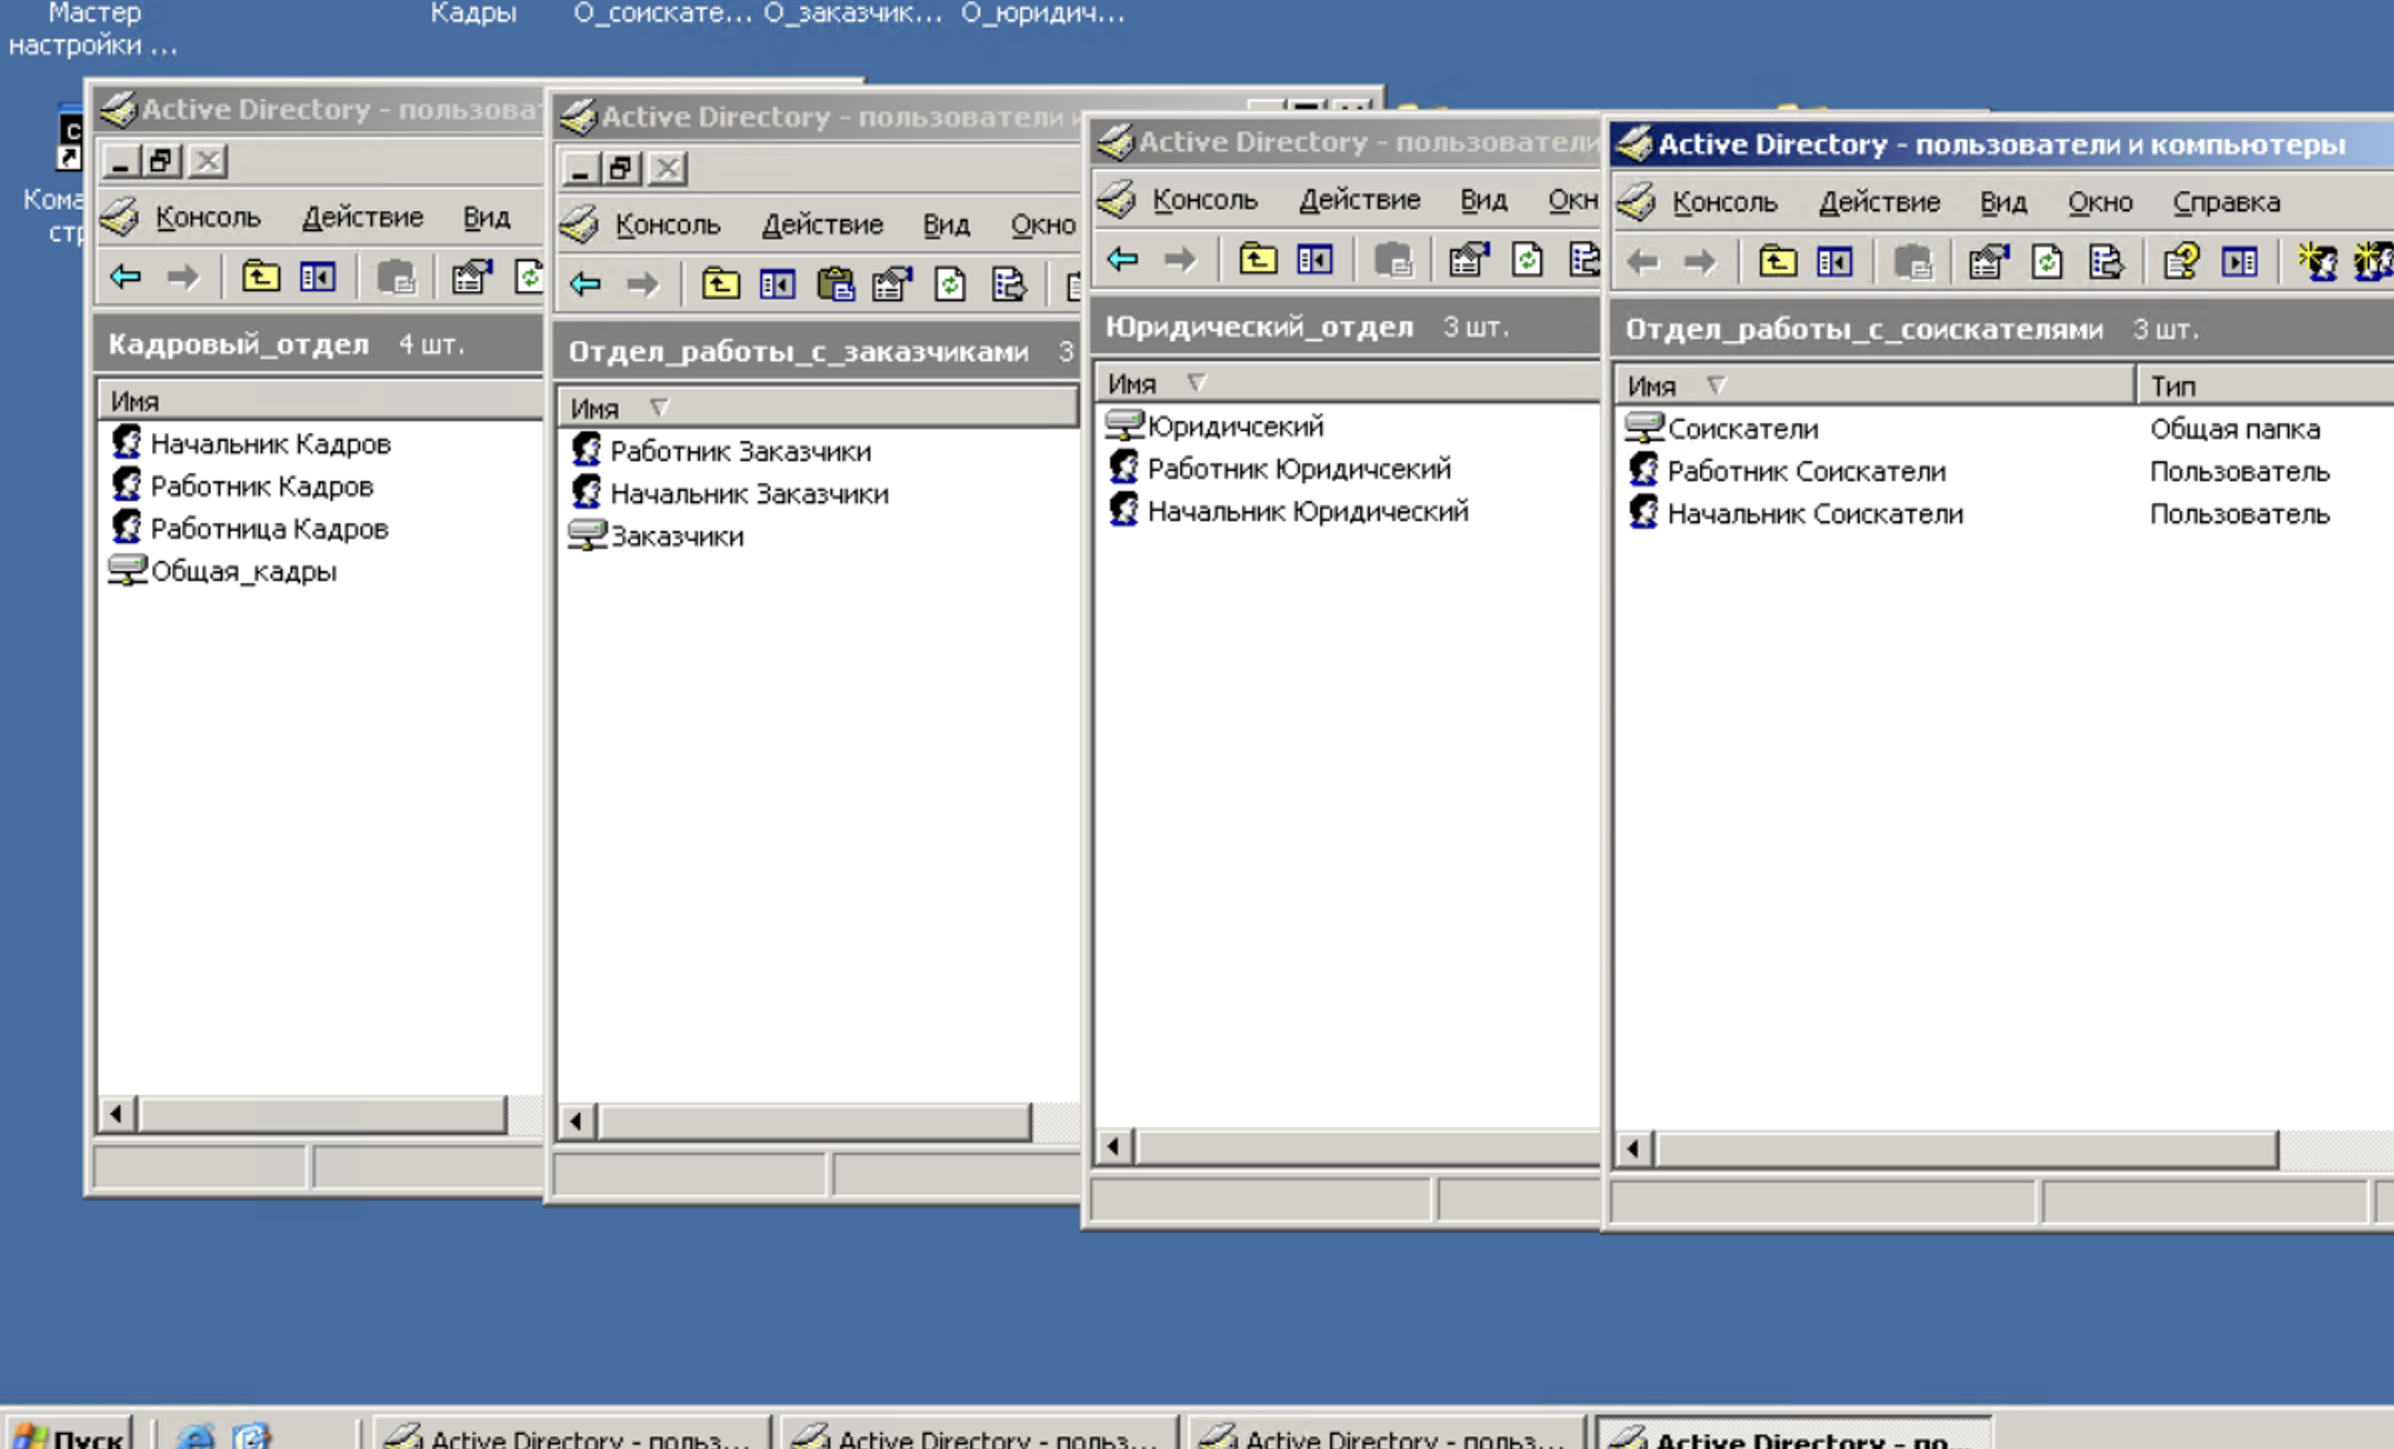
\includegraphics[width=0.9\textwidth]{pict/prac/7}
  \caption{Общие папки}
  \label{fig:18}
\end{figure}

Для своей папки, сотрудник имеет следующие права:
\begin{figure}[H]
  \centering
  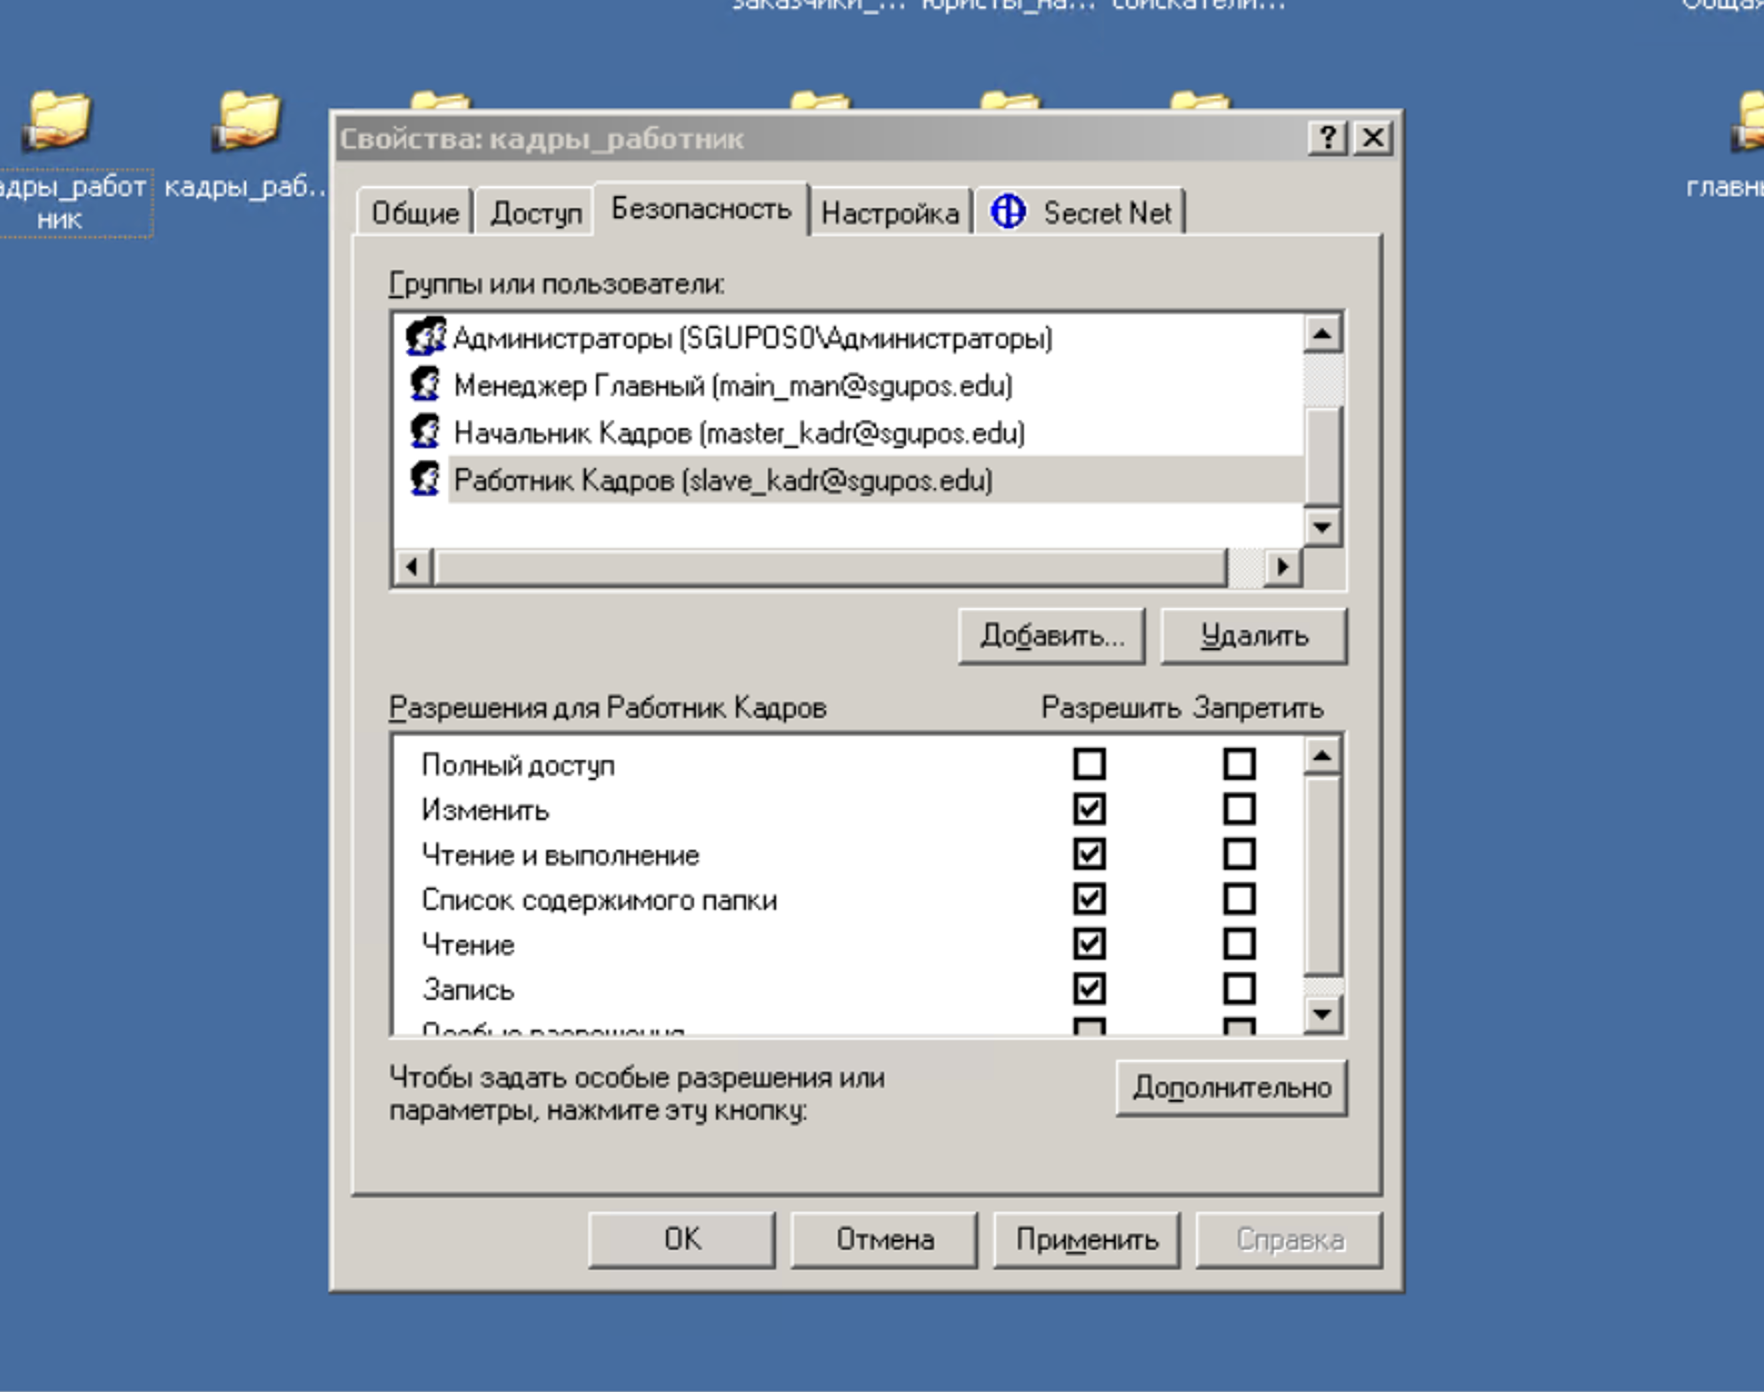
\includegraphics[width=0.9\textwidth]{pict/prac/8}
  \caption{Разрешено}
  \label{fig:20}
\end{figure}


\begin{figure}[H]
  \centering
  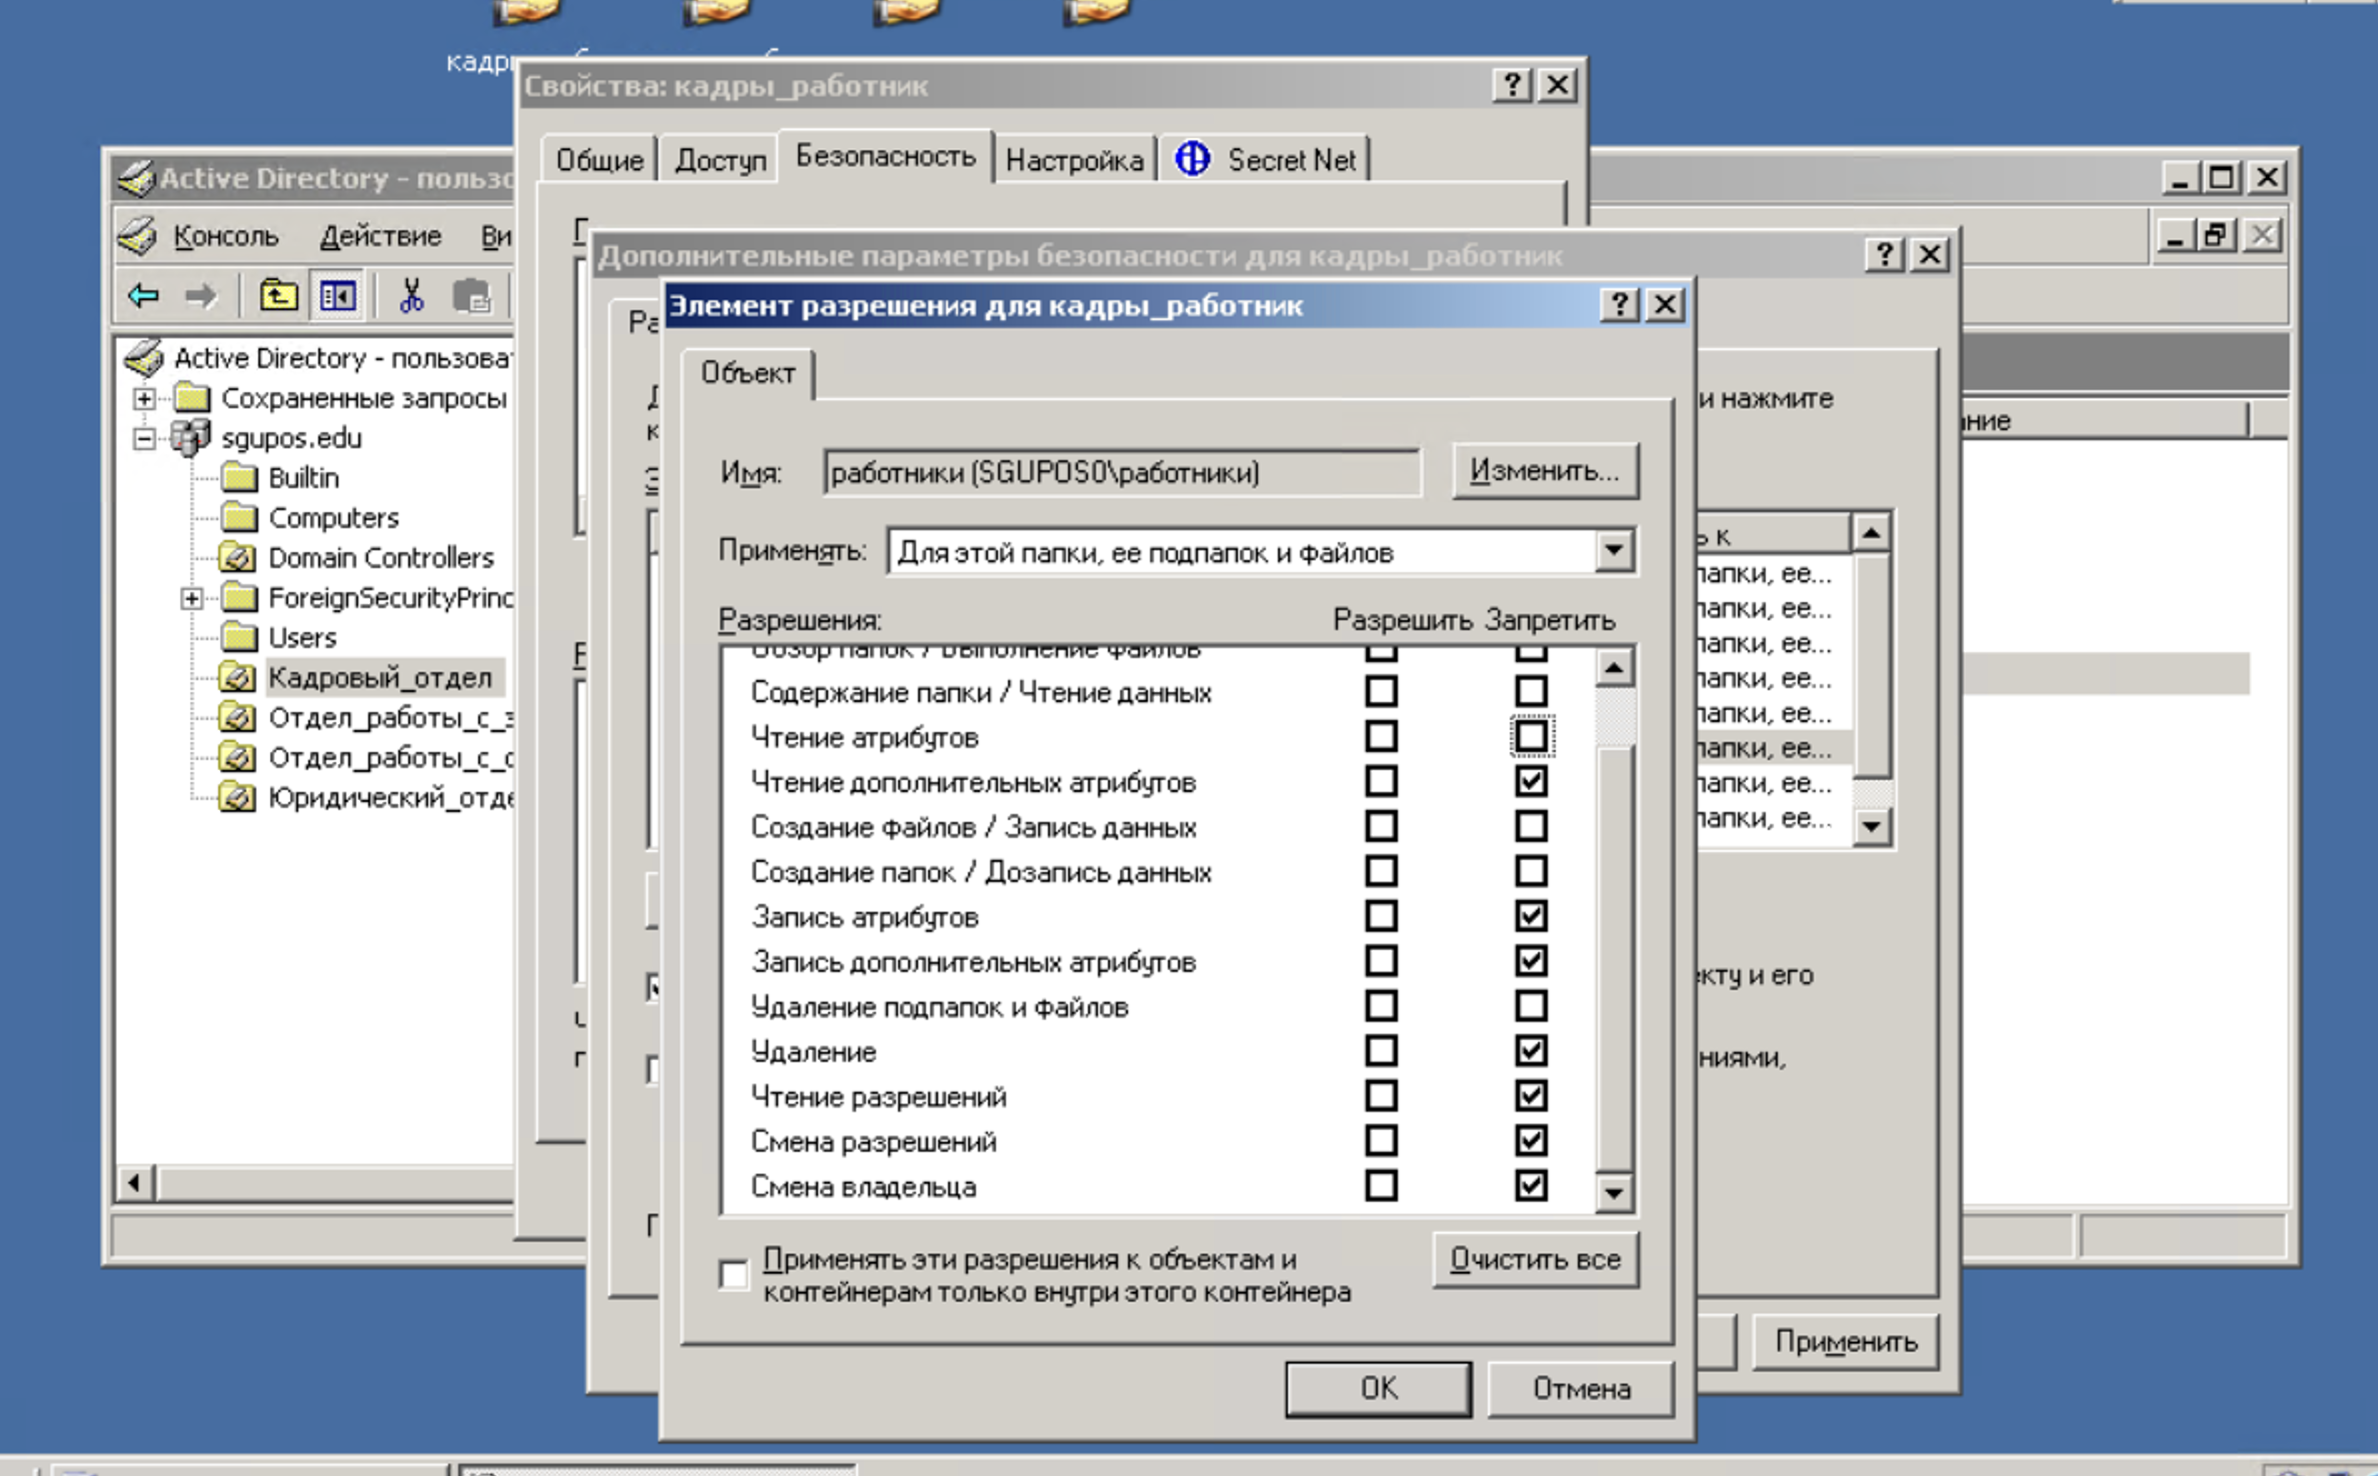
\includegraphics[width=0.9\textwidth]{pict/prac/61}
  \caption{Запрещено}
\end{figure}


Как мы видим полный доступ к папке имеет только администратор, он может менять владельца, права на доступ и т.д,
 что отвечает требованию к классу защищенности СВТ по ограничению прав для пользователей.
\begin{figure}[H]
    \centering
    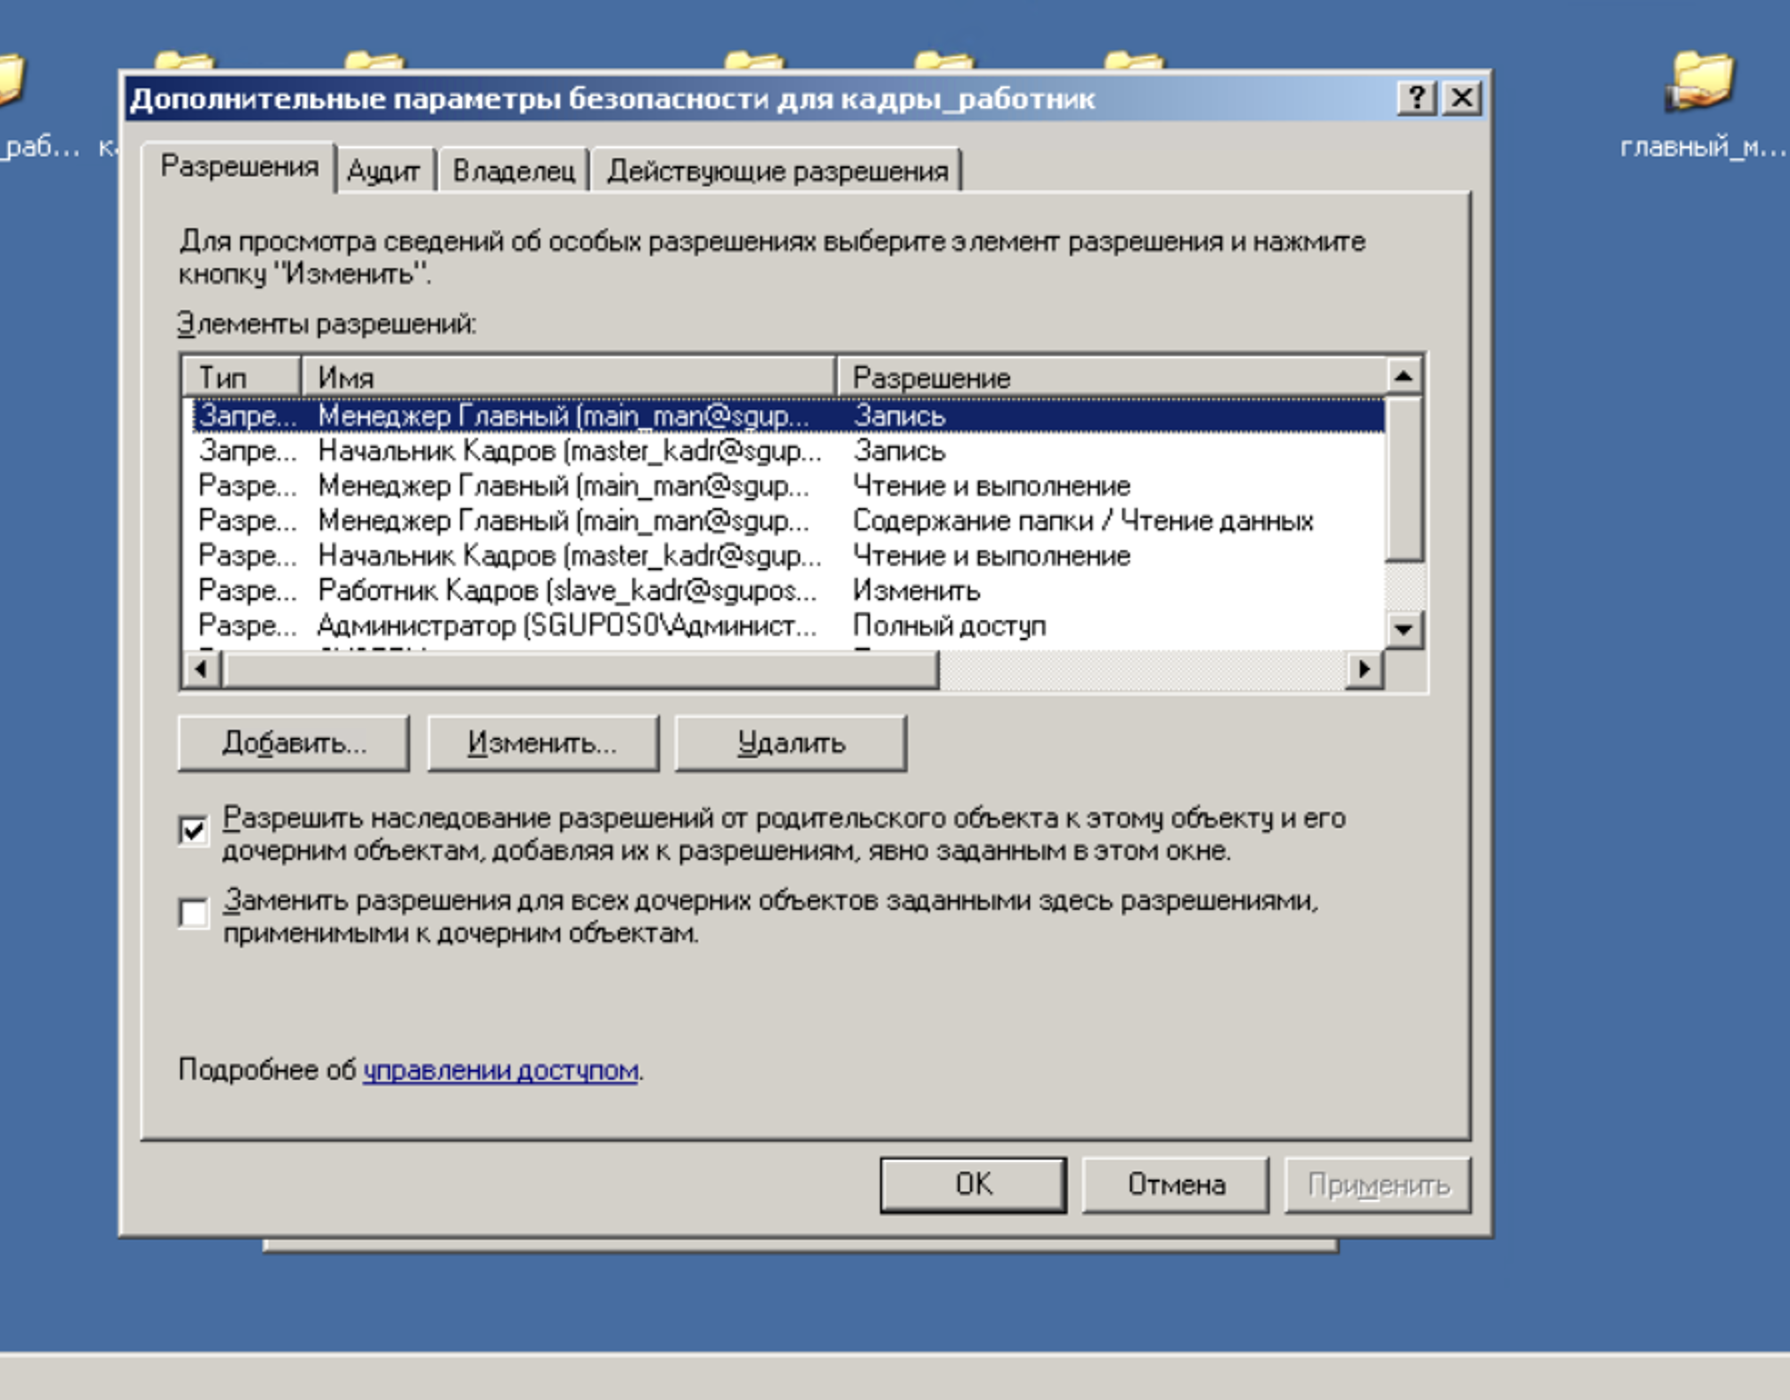
\includegraphics[width=1\textwidth]{pict/prac/9}
    \caption{Права на папку сотрудника}
    \label{fig:21}
\end{figure}

\begin{figure}[H]
  \centering
  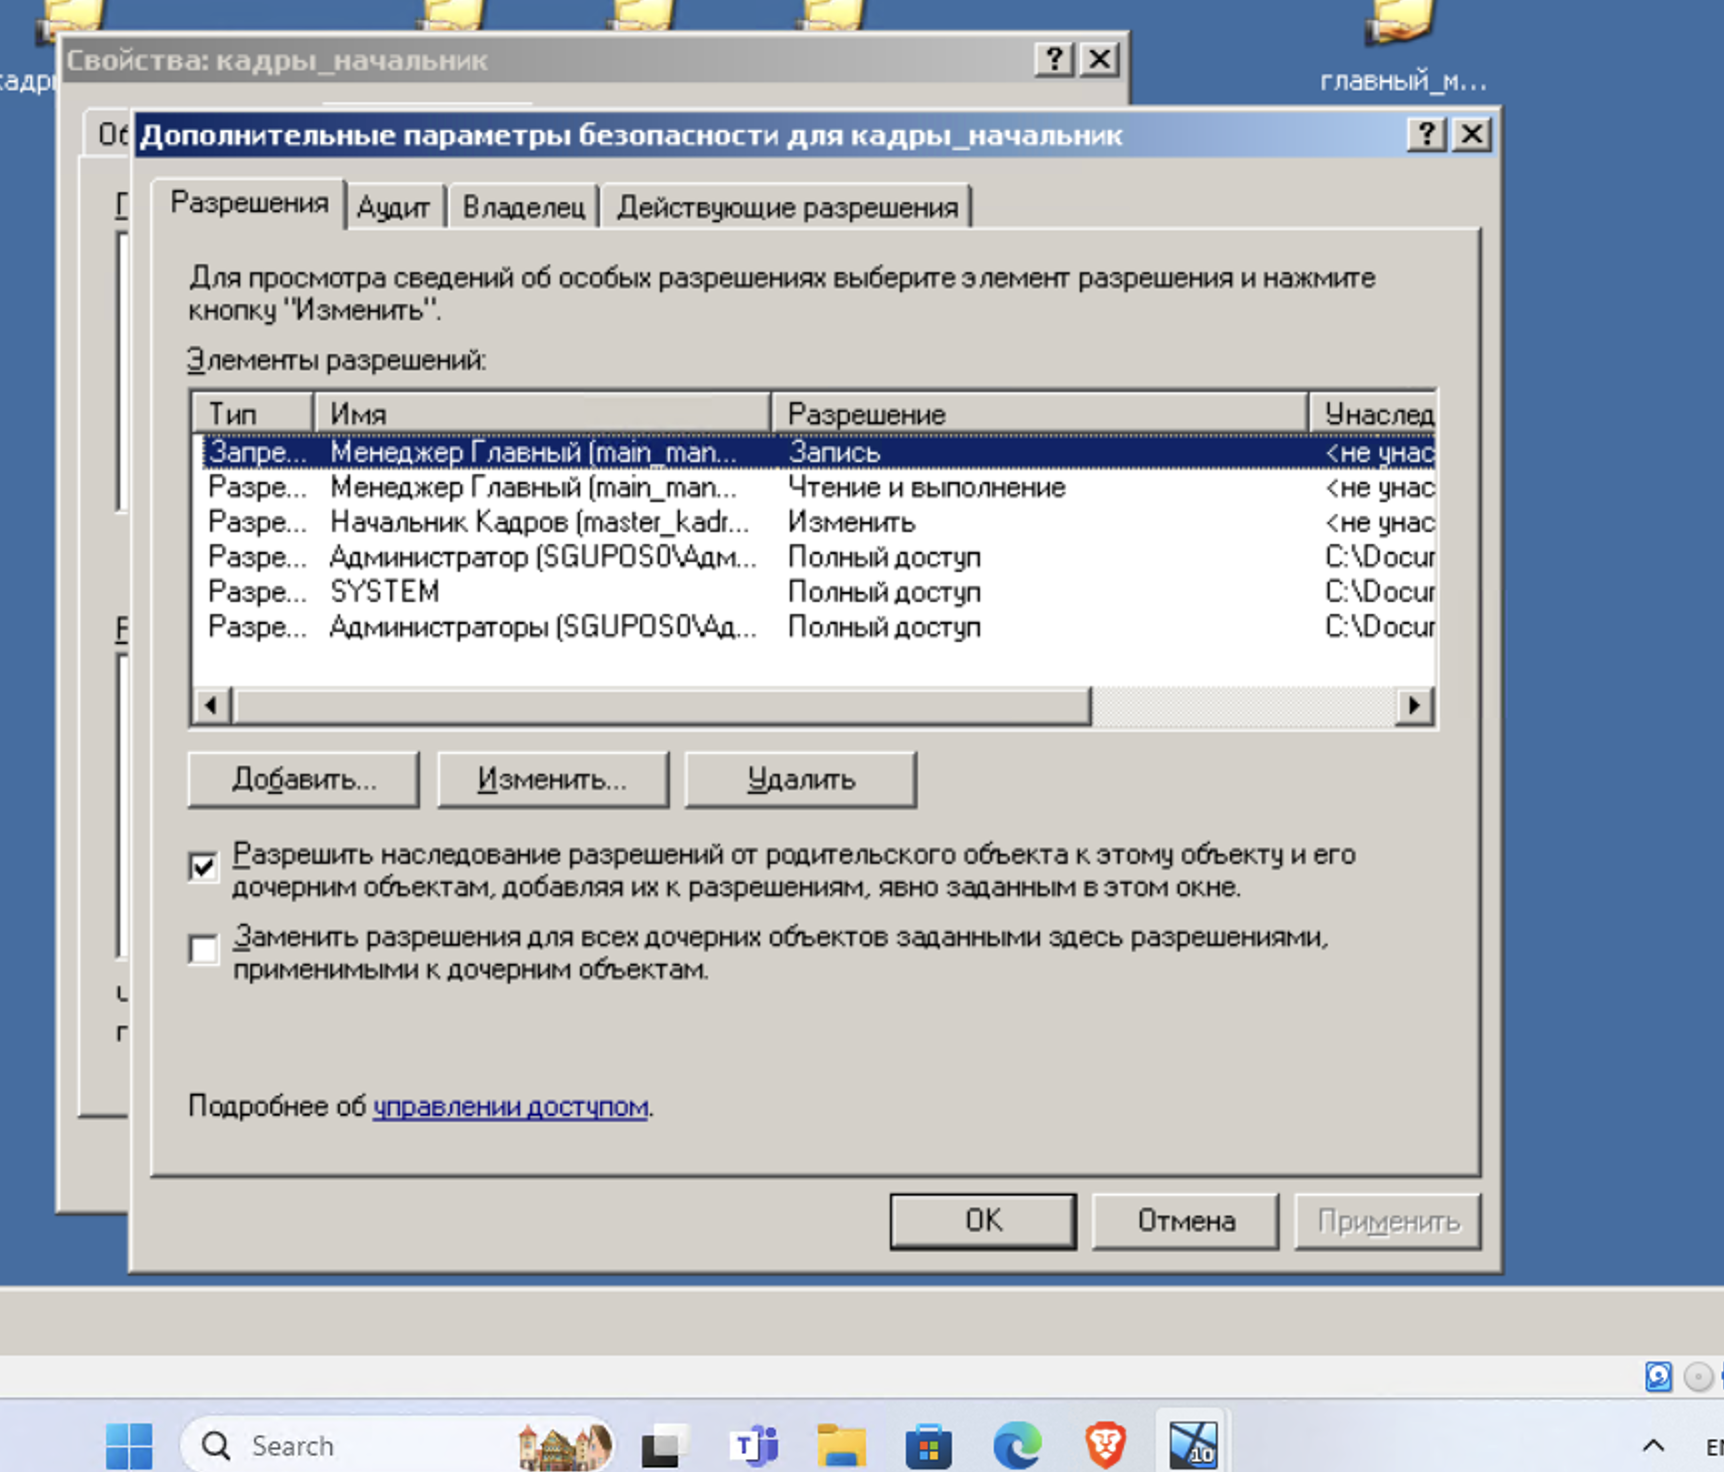
\includegraphics[width=1\textwidth]{pict/prac/10}
  \caption{Права на папку начальника}
  \label{fig:22}
\end{figure}

\newpage
К папке главного менеджера доступ и права имеет только сам менеджер.
\begin{figure}[H]
  \centering
  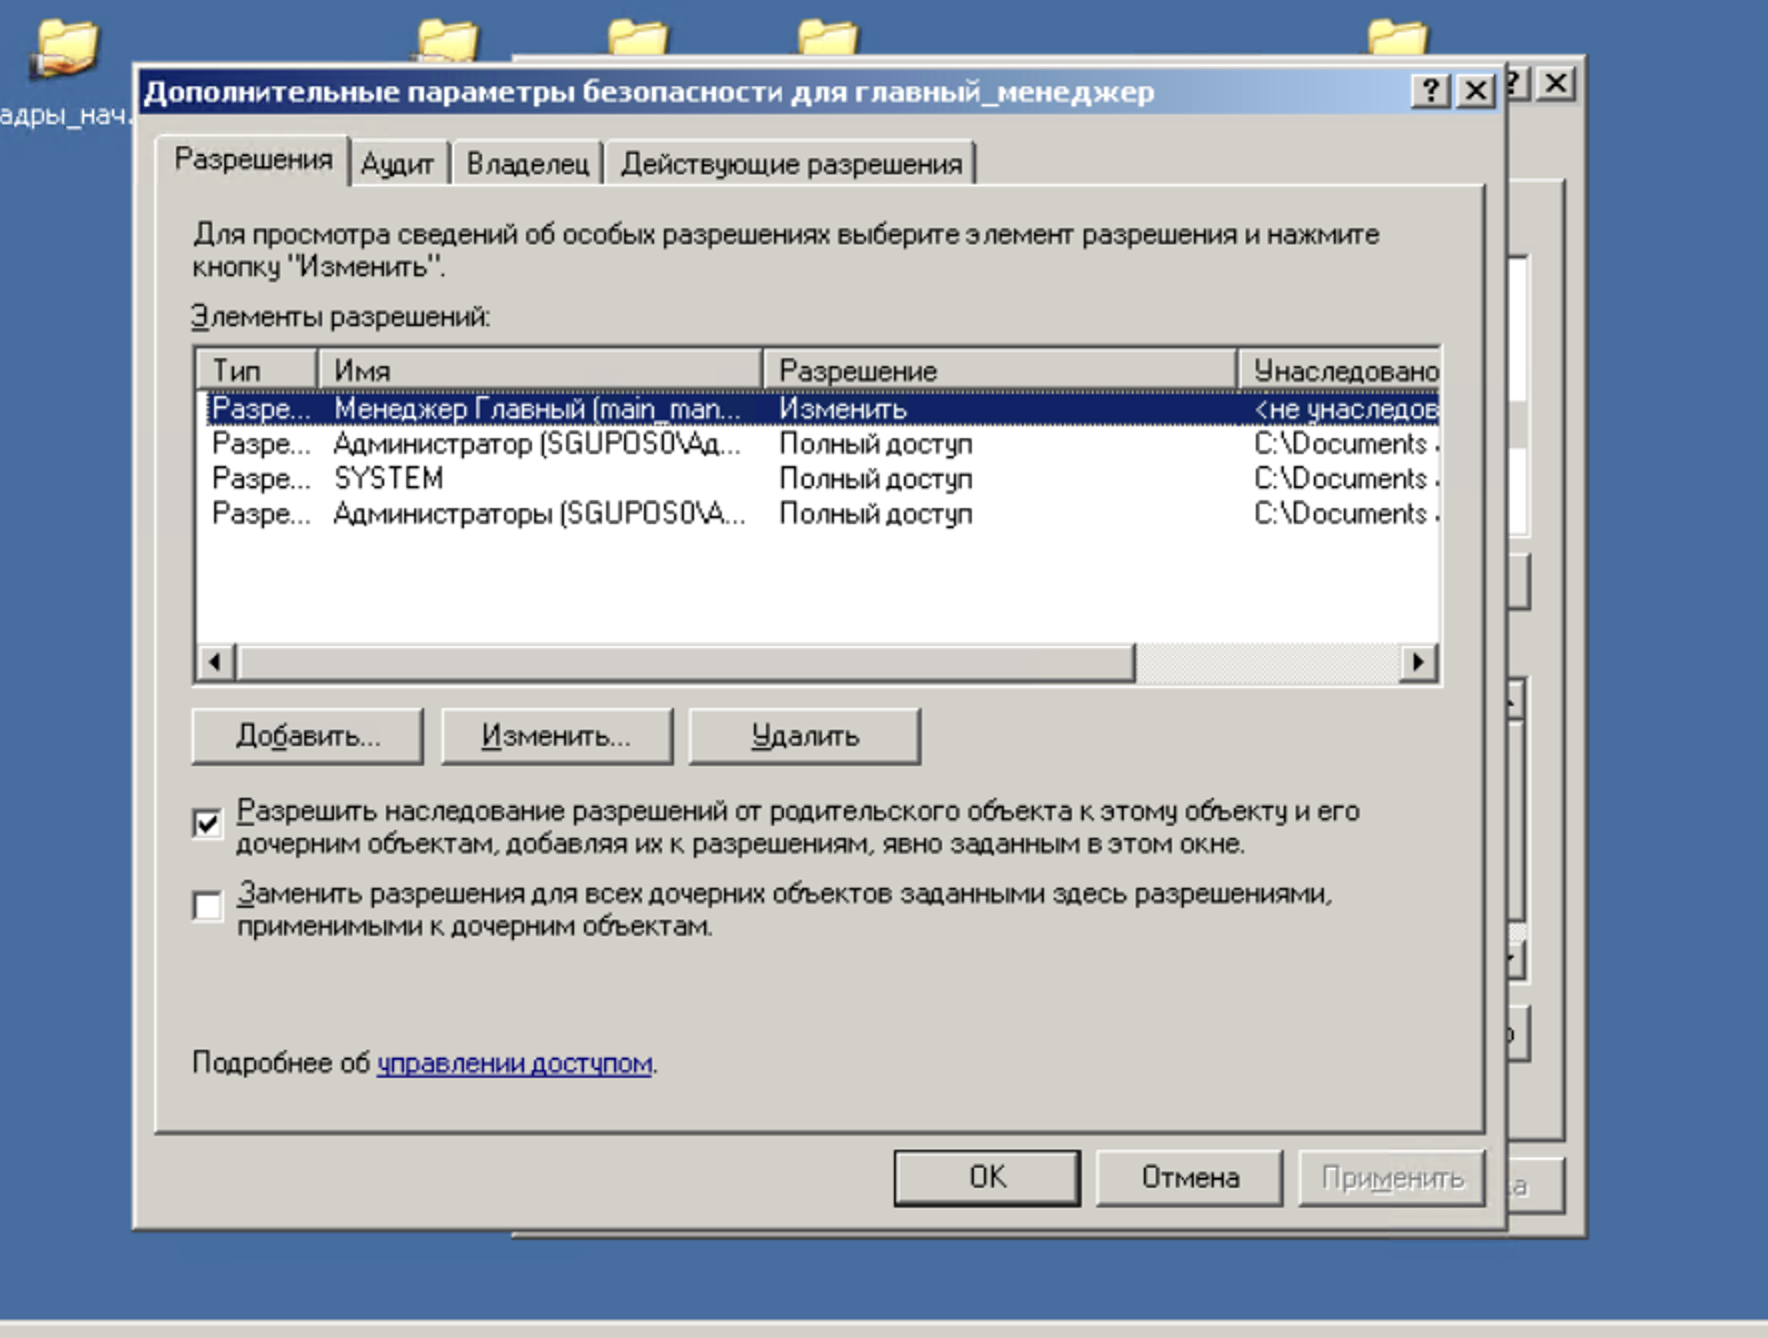
\includegraphics[width=1\textwidth]{pict/prac/11}
  \caption{Права на папку главного менеджера}
  \label{fig:48}
\end{figure}
Настроем аналогичные правила для аккаунтов всех остальных подразделений.

\newpage


\subsubsection{Проверка работы настроек}

Зайдем в учетную запись работника кадров, проверим доступность.
\begin{figure}[H]
  \centering
  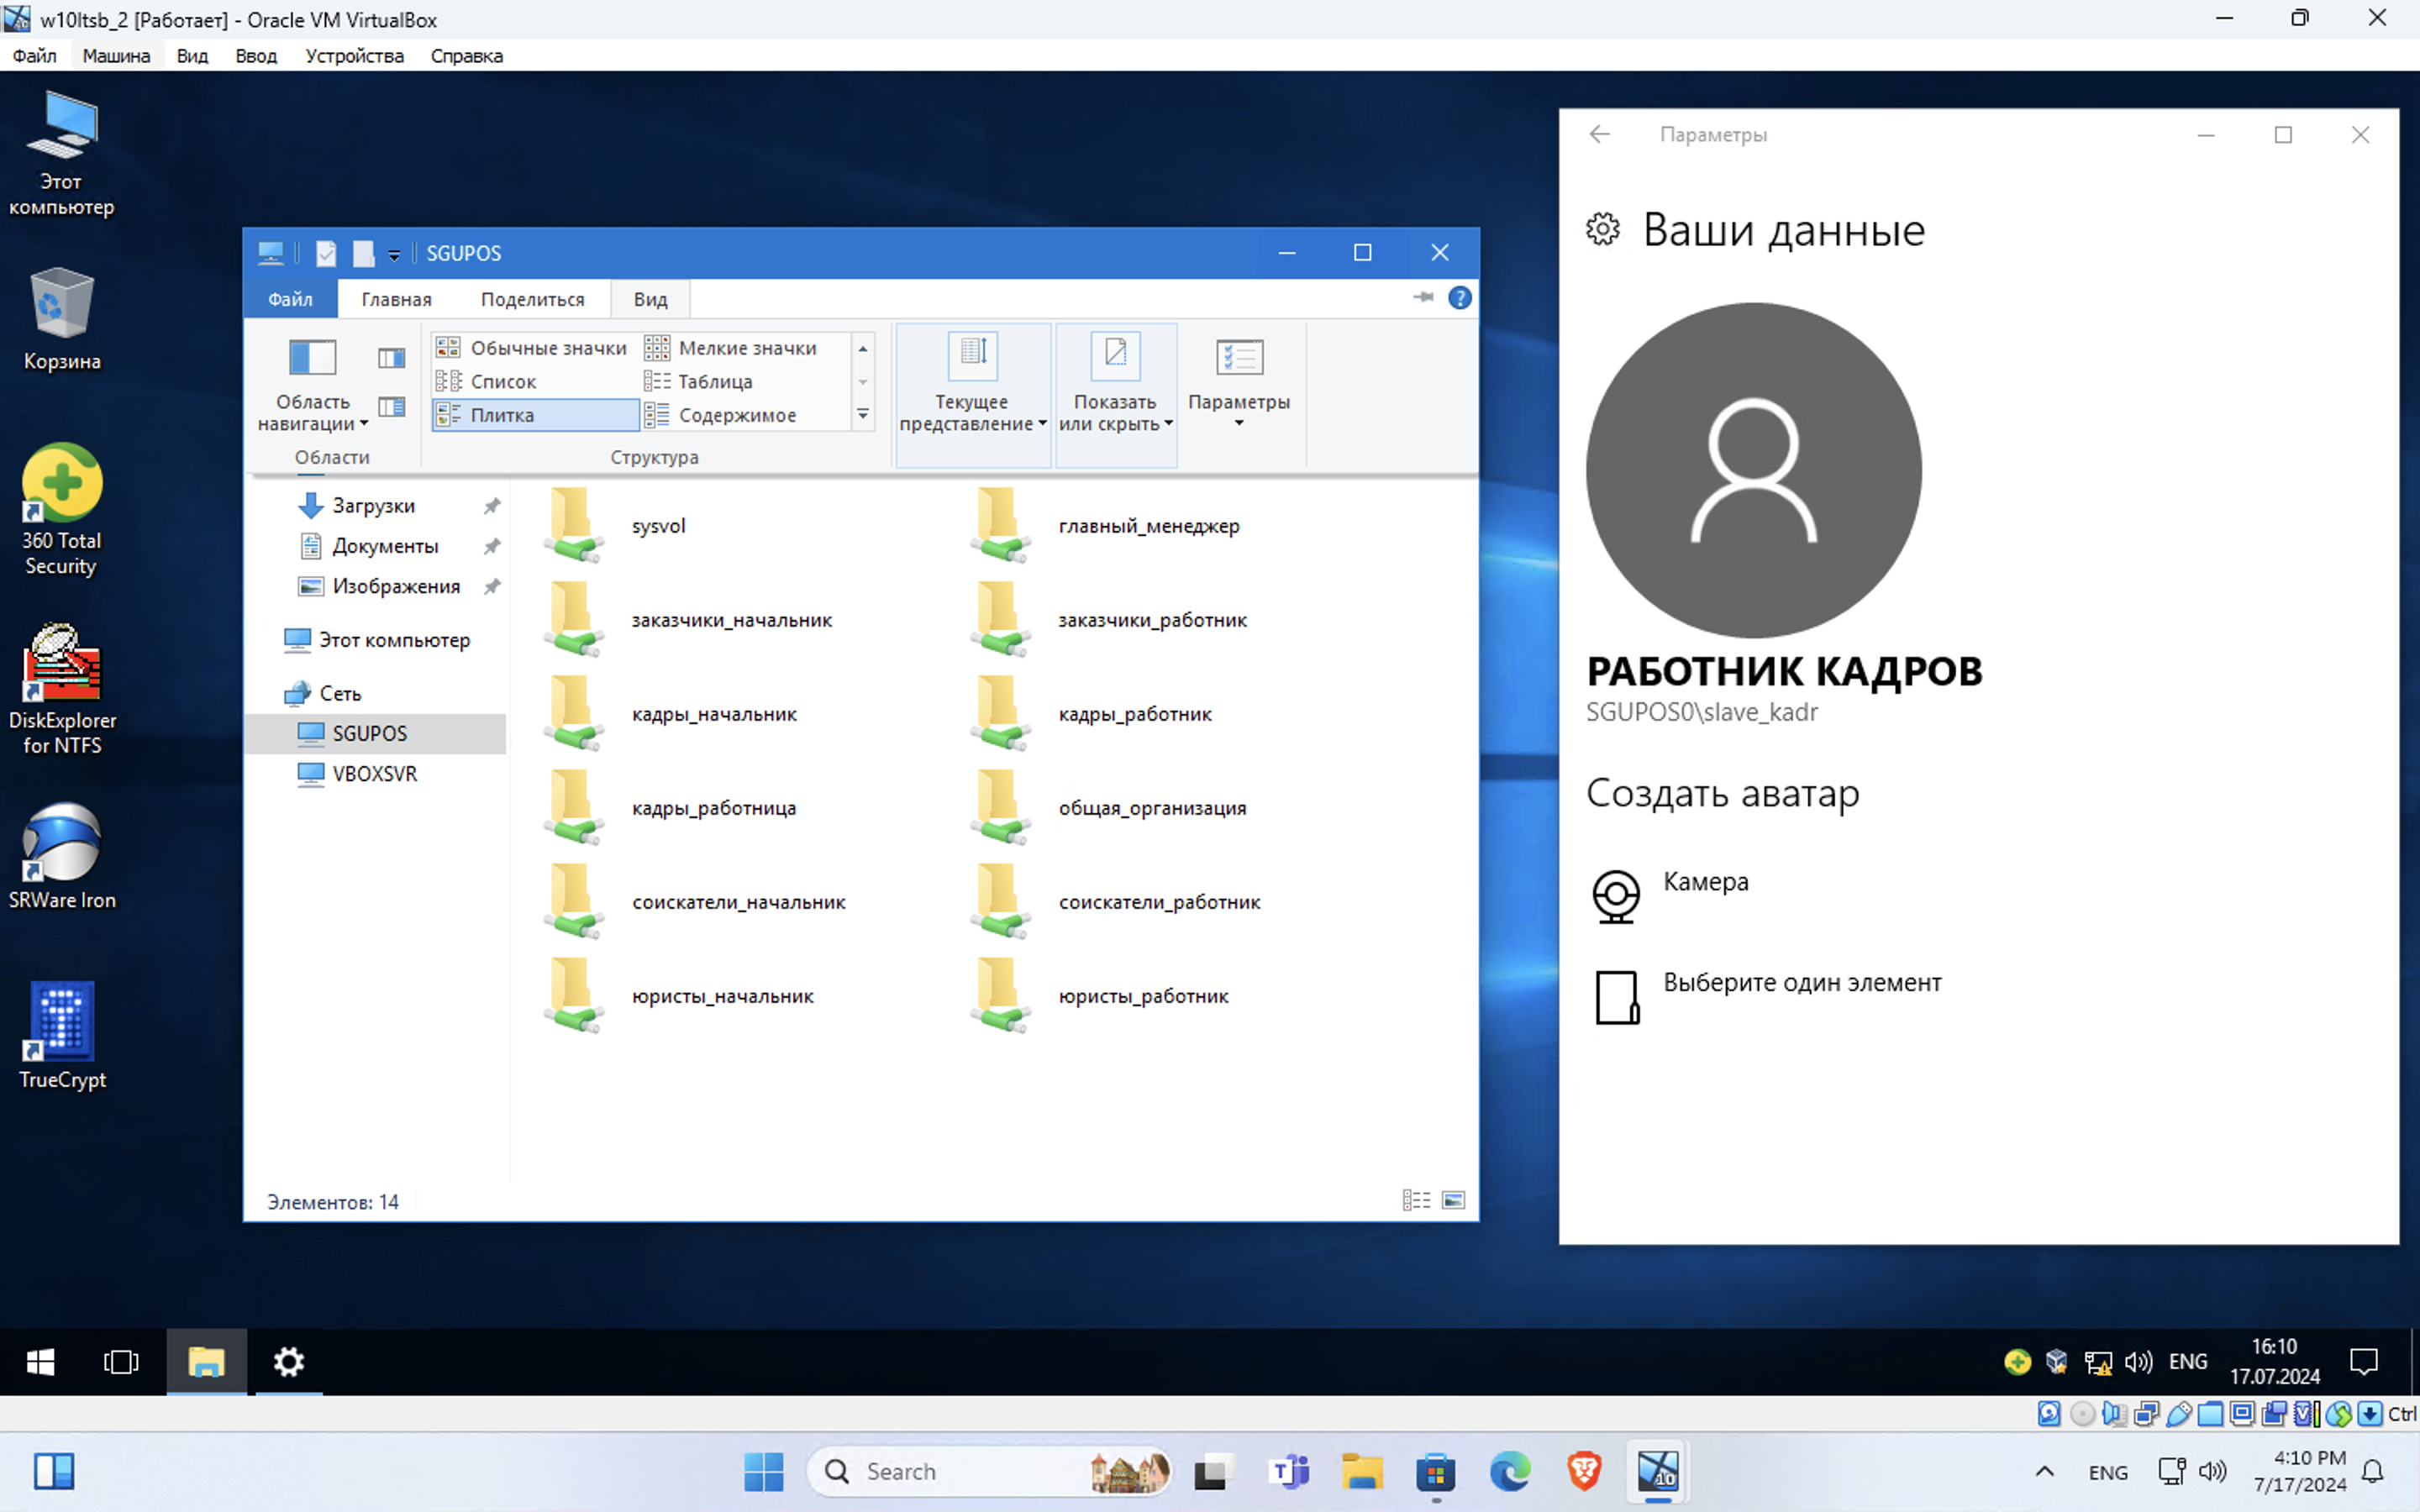
\includegraphics[width=0.9\textwidth]{pict/prac/25}
  \caption{Аккаунт работника кадров}
  \label{fig:24}
\end{figure}

\begin{figure}[H]
  \centering
  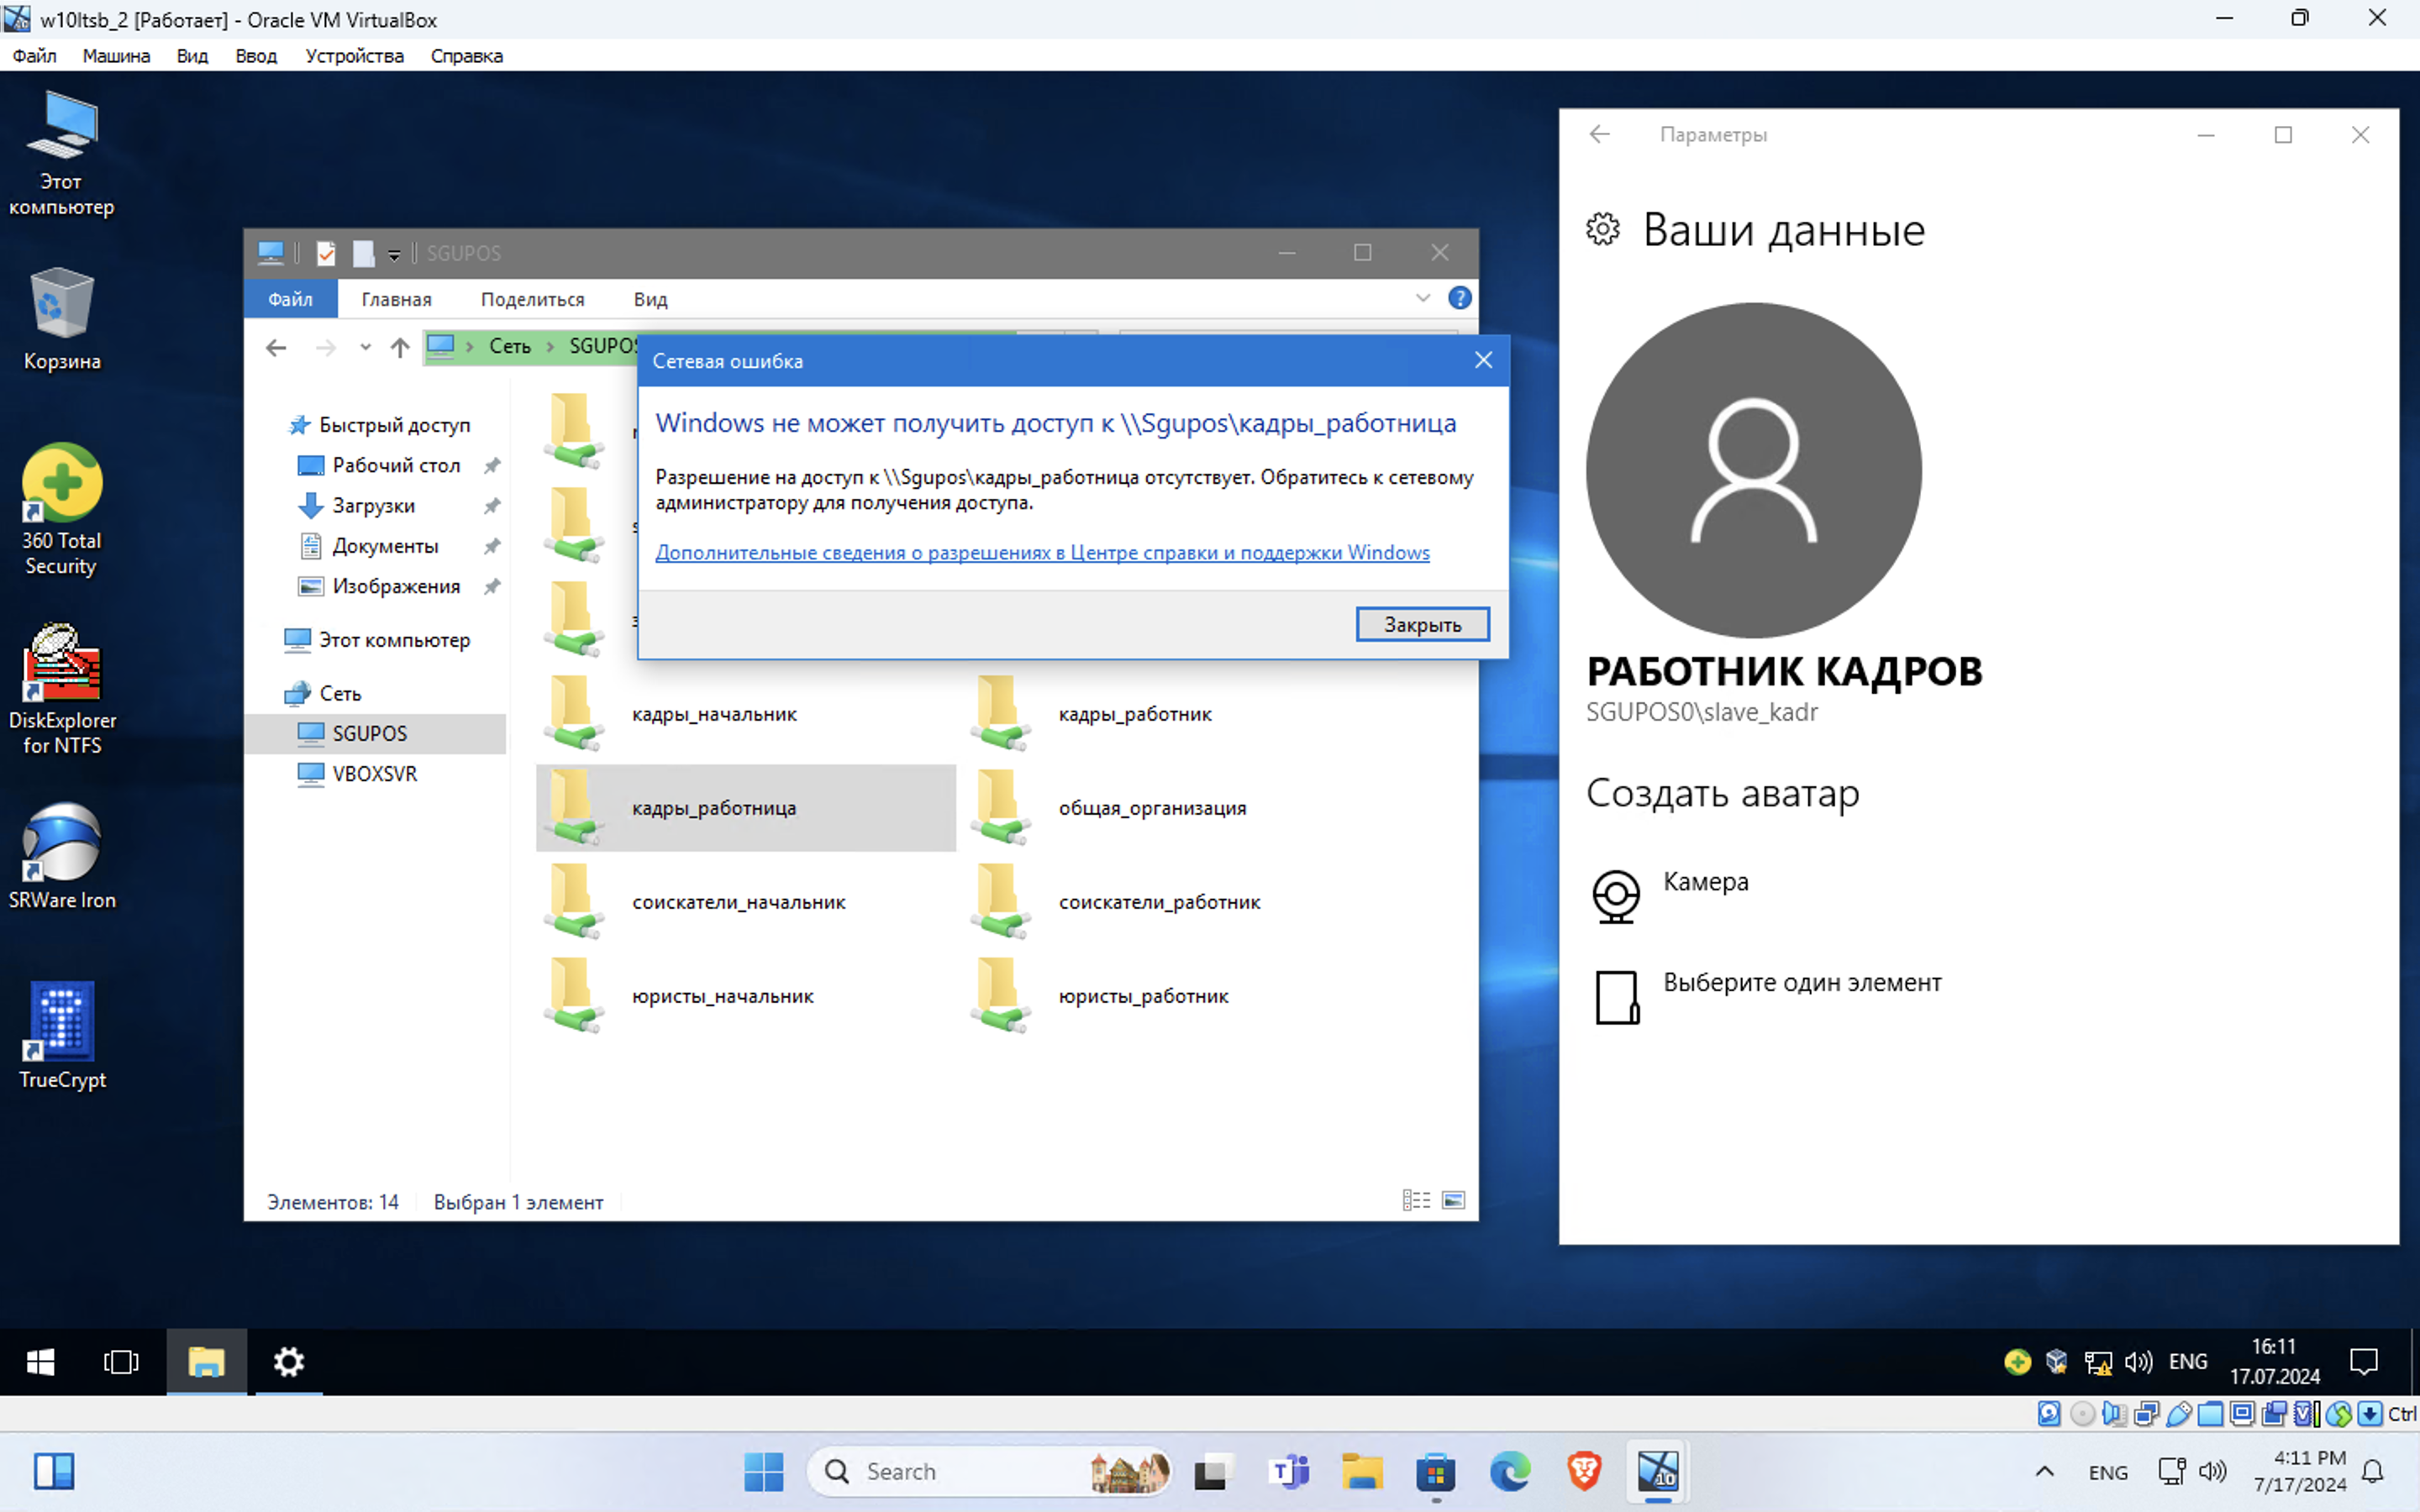
\includegraphics[width=0.9\textwidth]{pict/prac/26}
  \caption{Работник кадров -> Работница кадров}
  \label{fig:25}
\end{figure}


\begin{figure}[H]
  \centering
  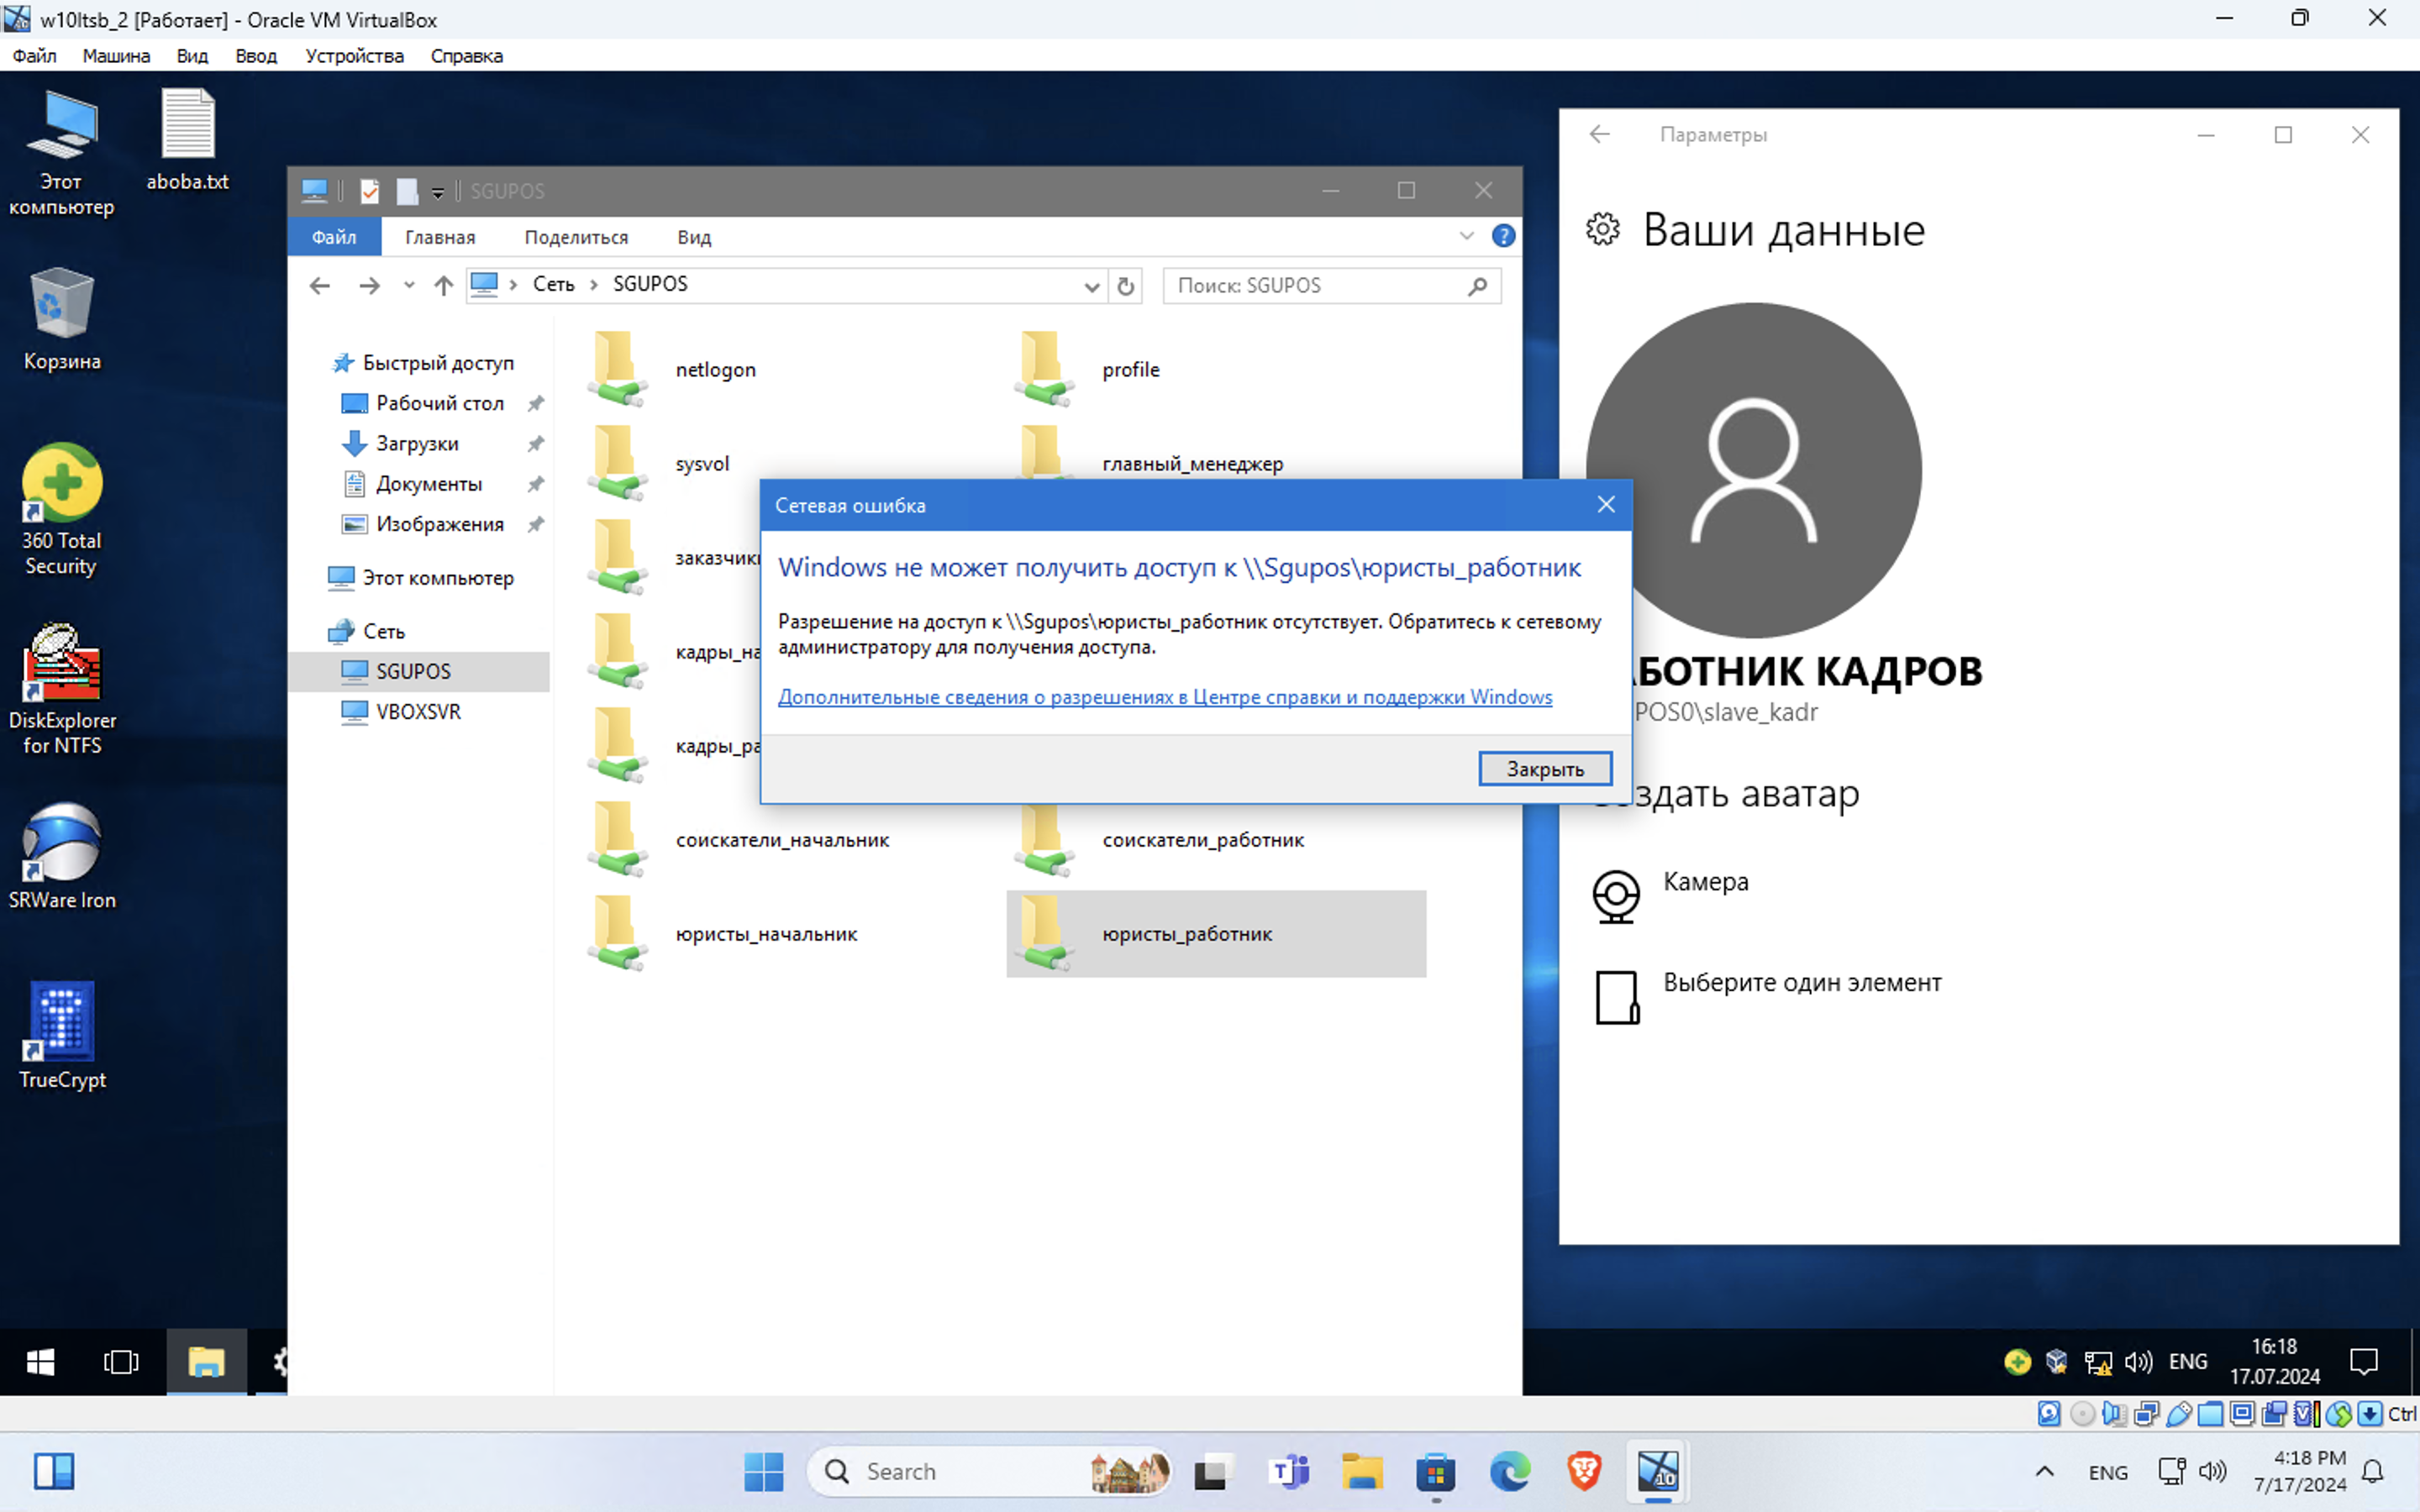
\includegraphics[width=1\textwidth]{pict/prac/32}
  \caption{Работник кадров -> Работник юристов}
  \label{fig:31}
\end{figure}


\begin{figure}[H]
  \centering
  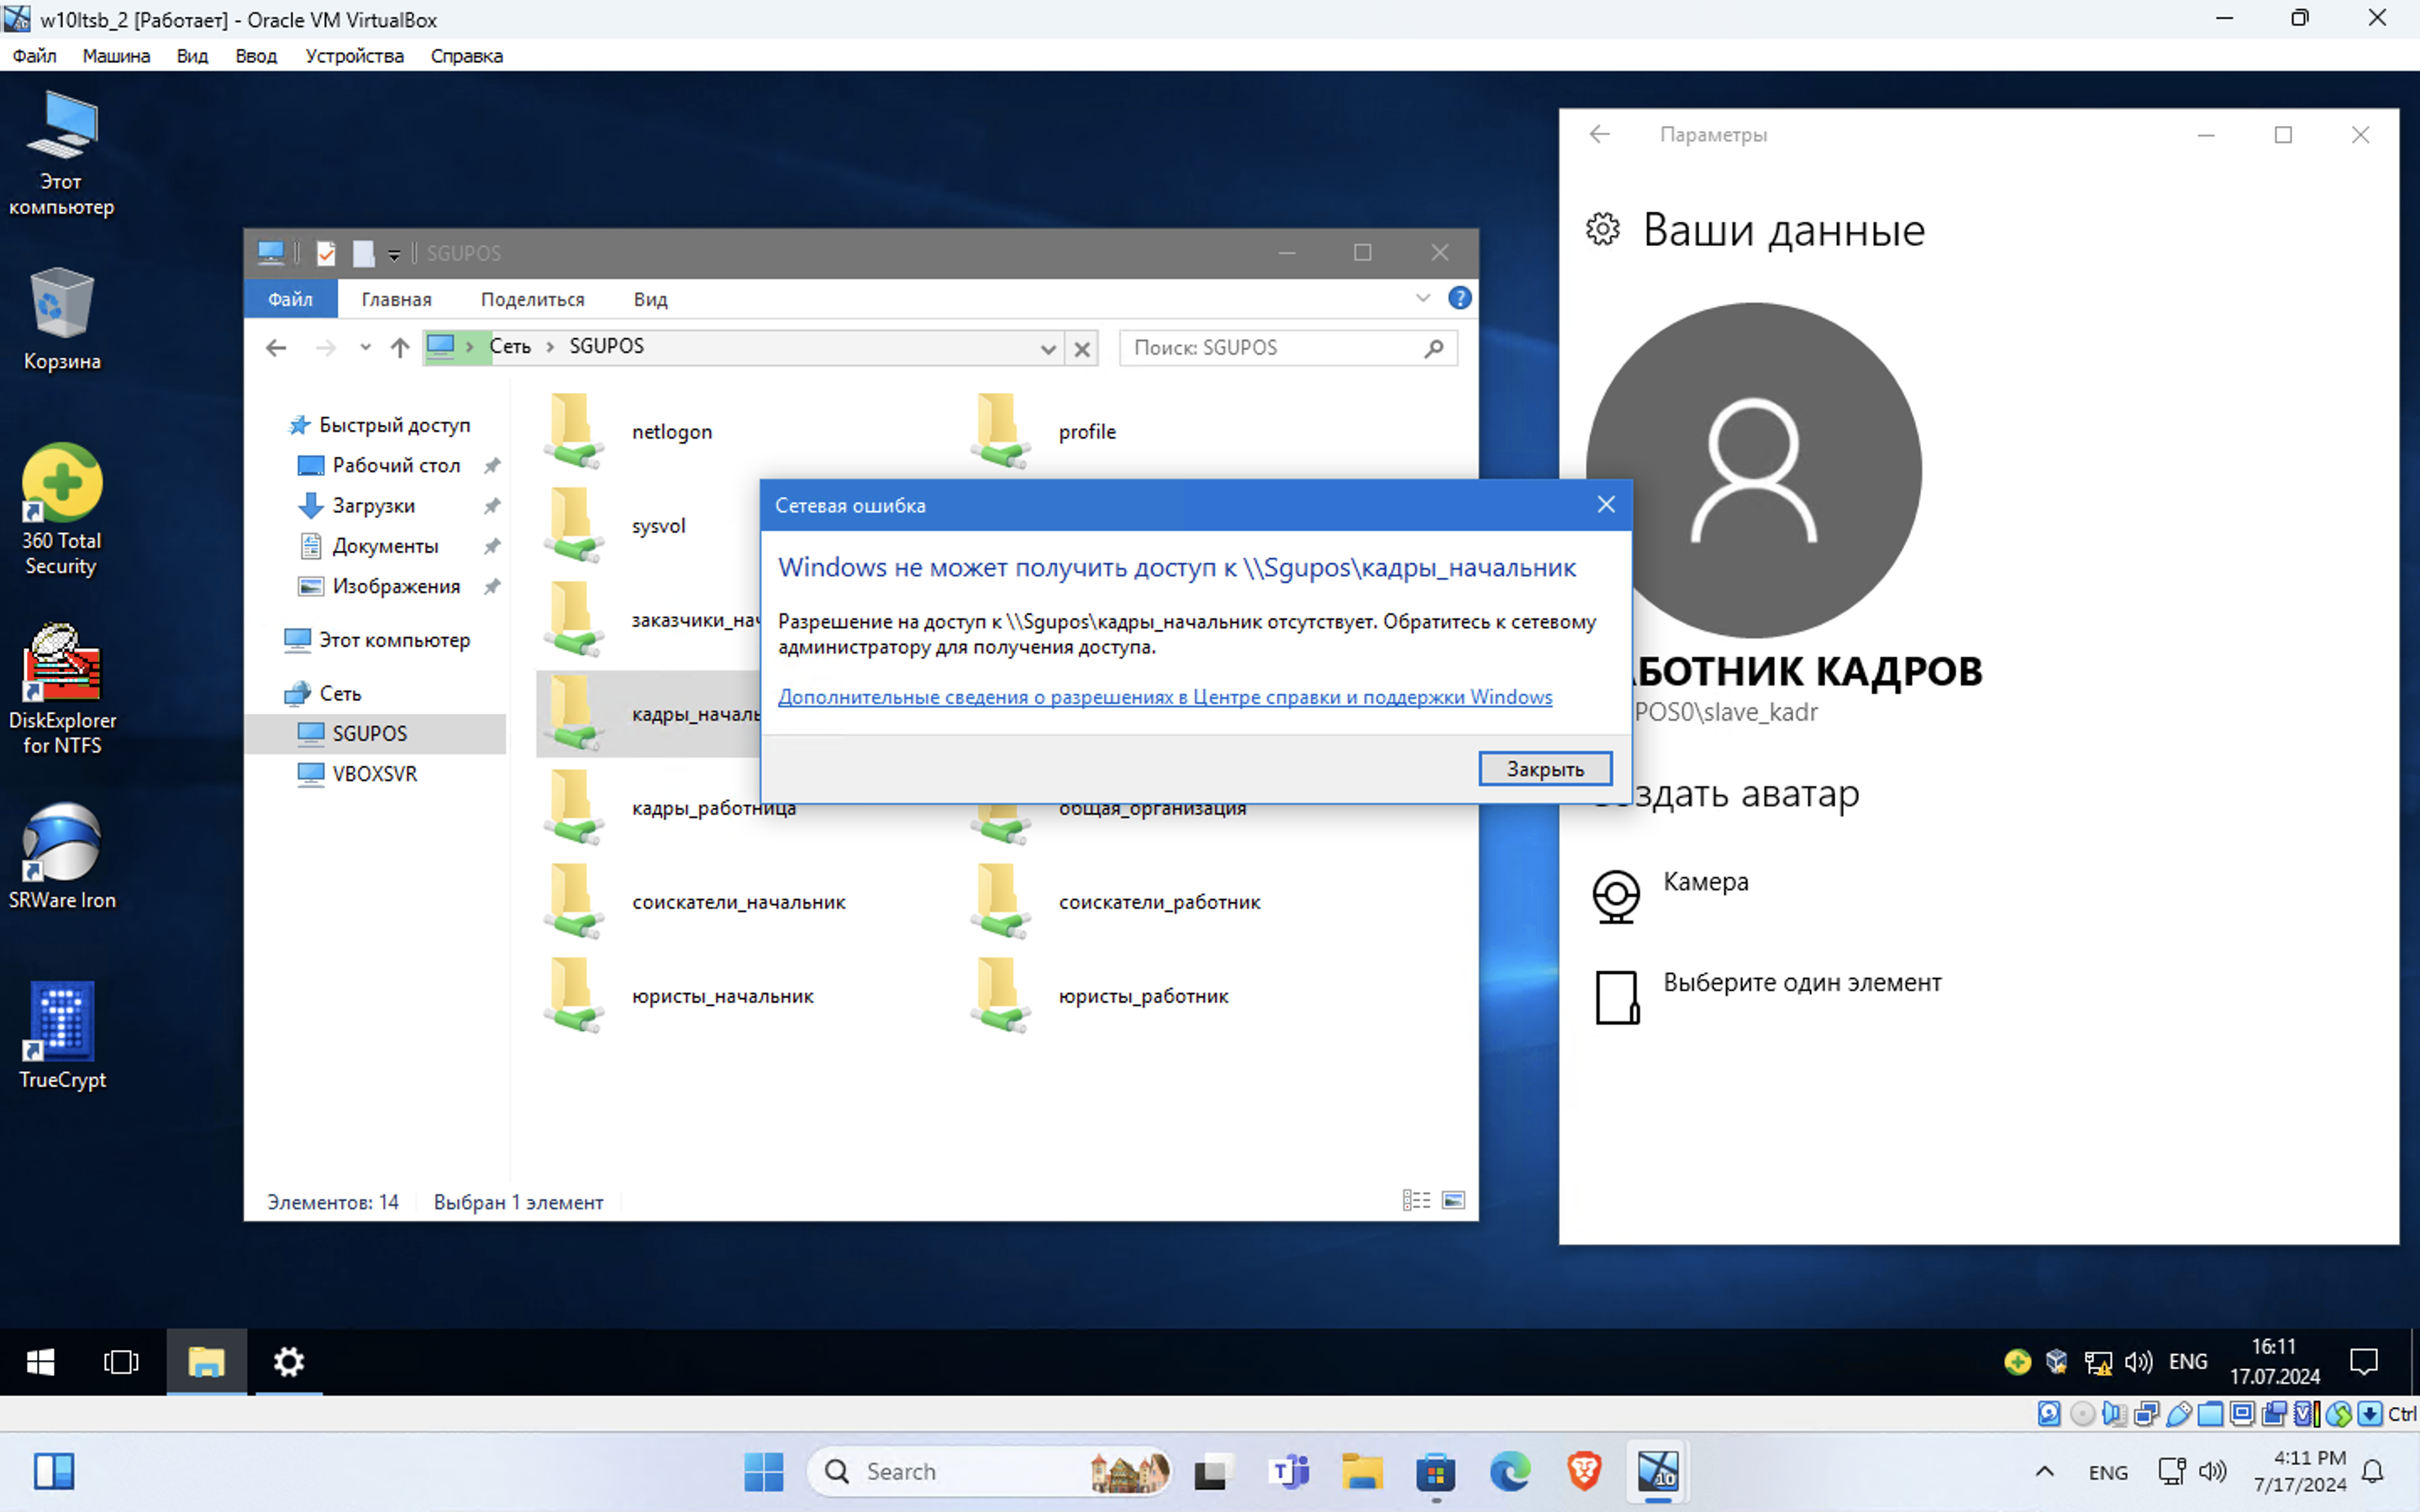
\includegraphics[width=1\textwidth]{pict/prac/27}
  \caption{Работник кадров -> Начальник кадров}
  \label{fig:26}
\end{figure}


\begin{figure}[H]
  \centering
  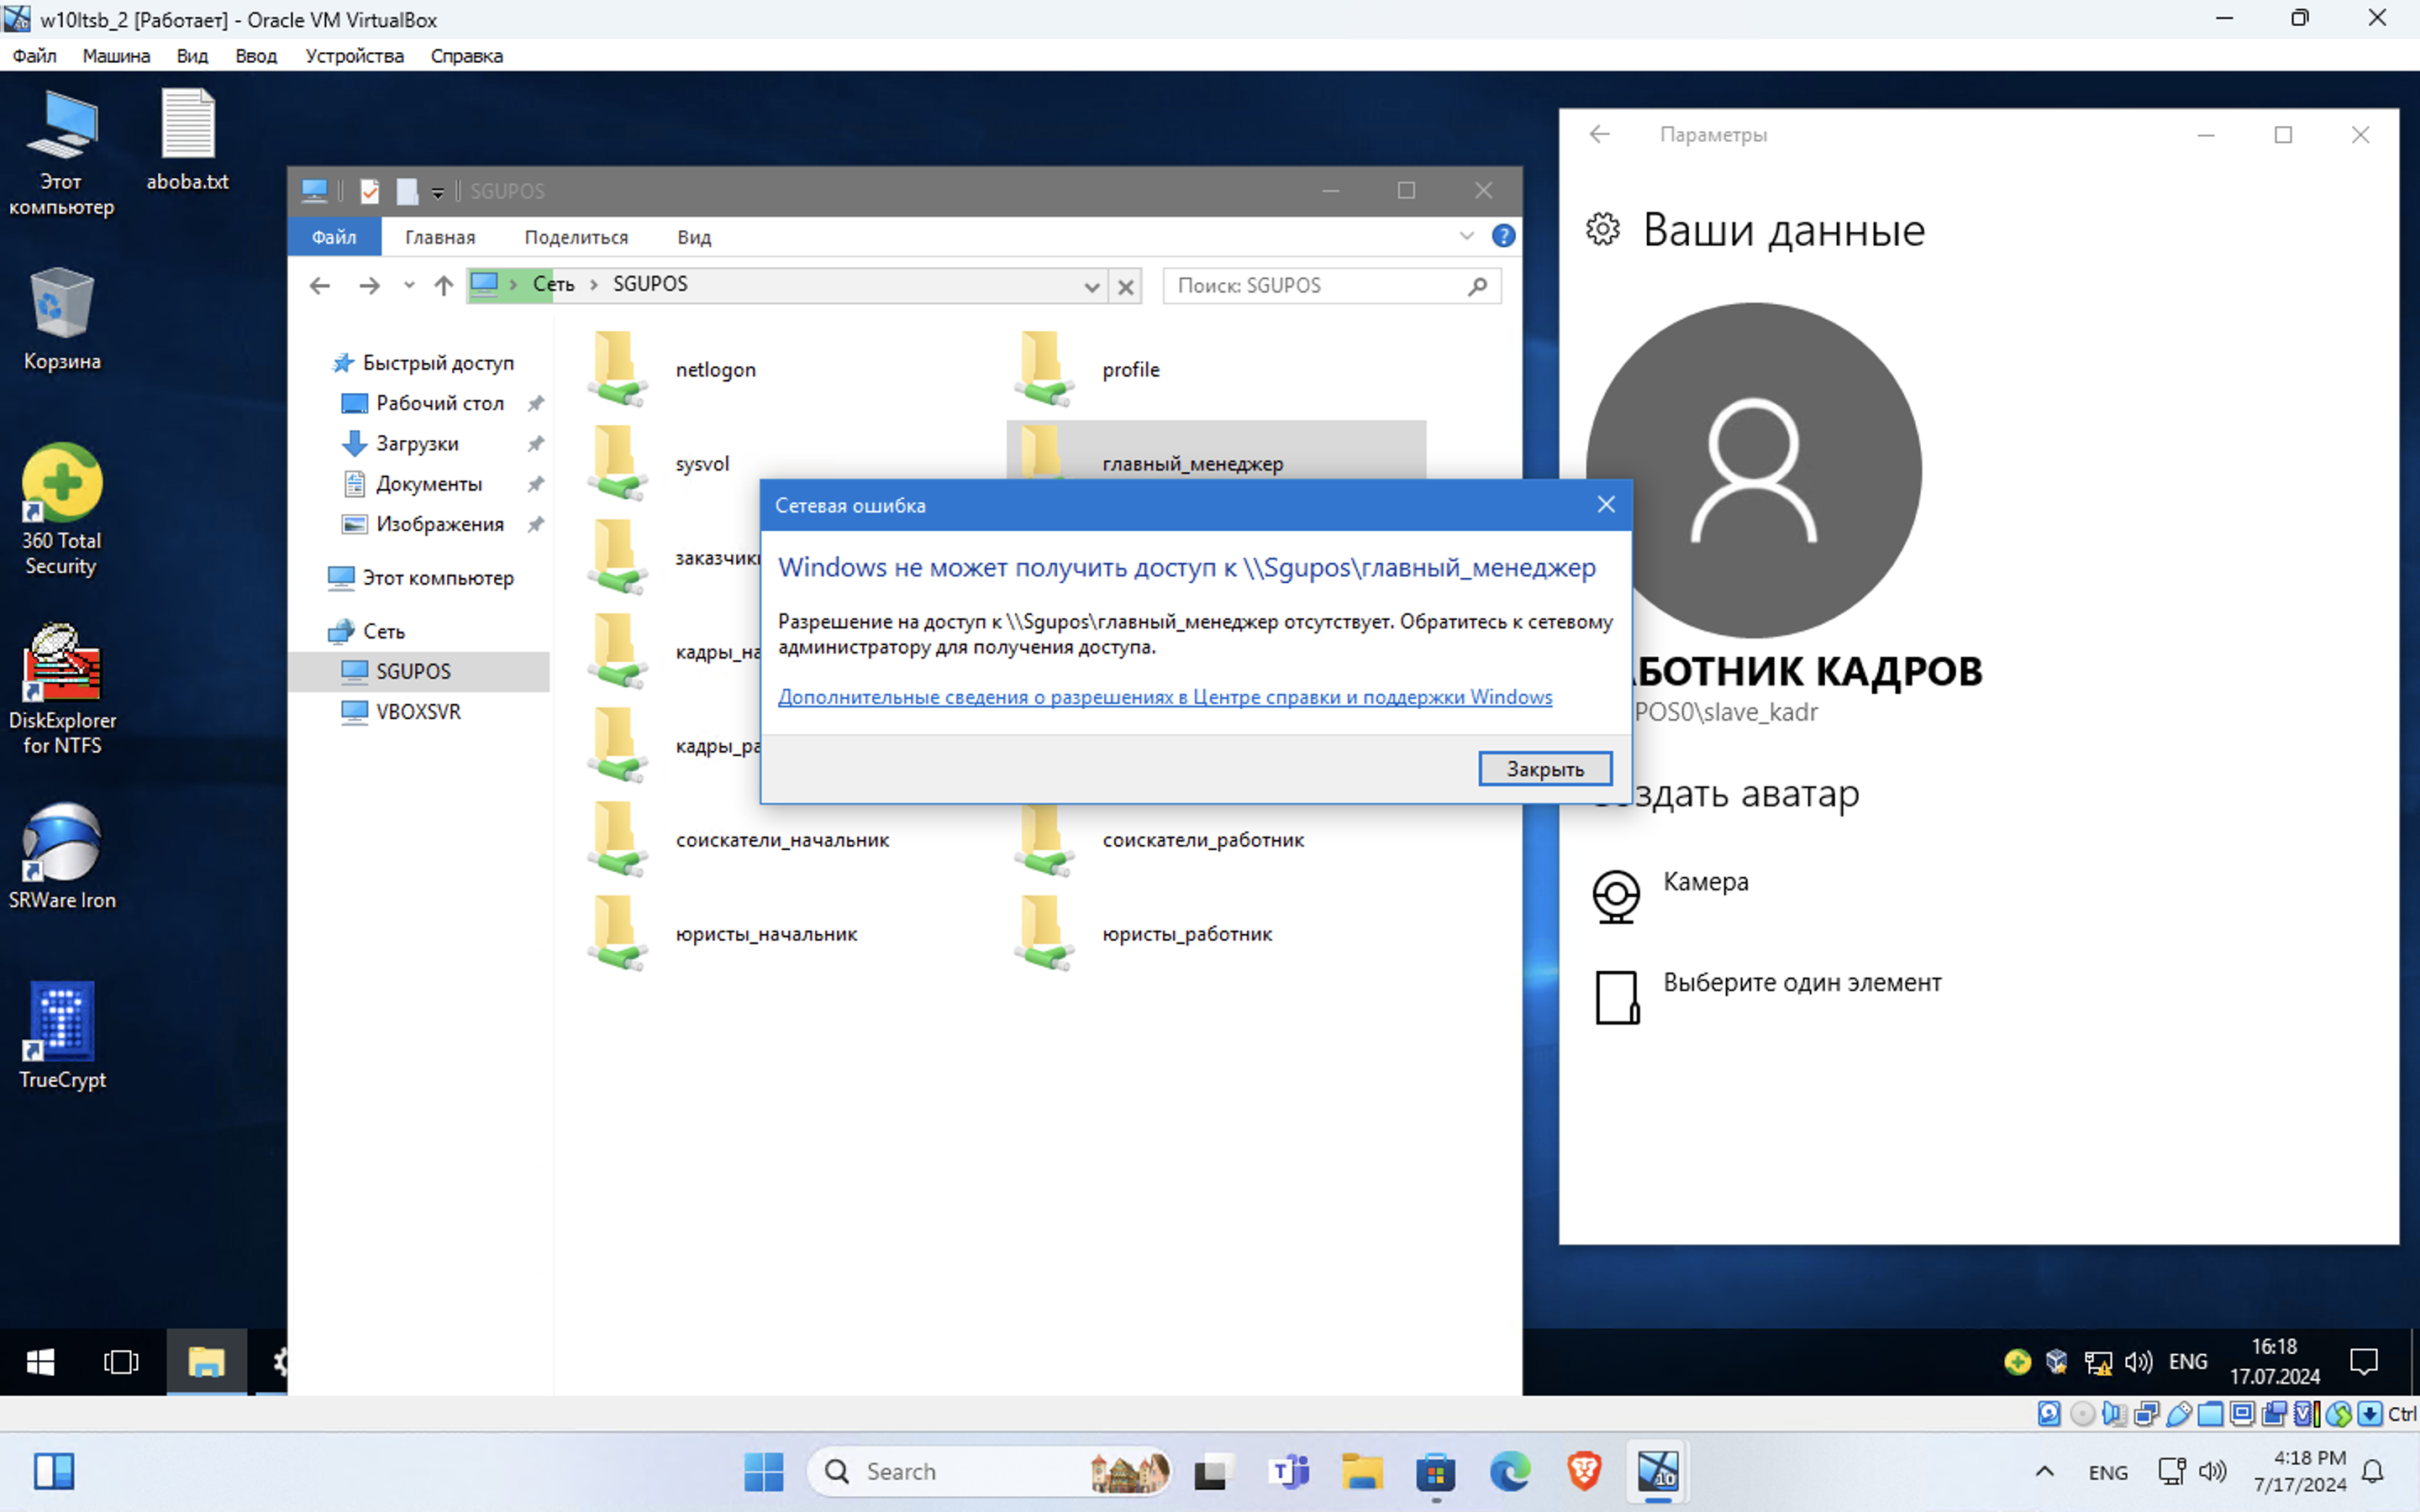
\includegraphics[width=1\textwidth]{pict/prac/31}
  \caption{Работник кадров -> Главный менеджер}
  \label{fig:30}
\end{figure}

\begin{figure}[H]
  \centering
  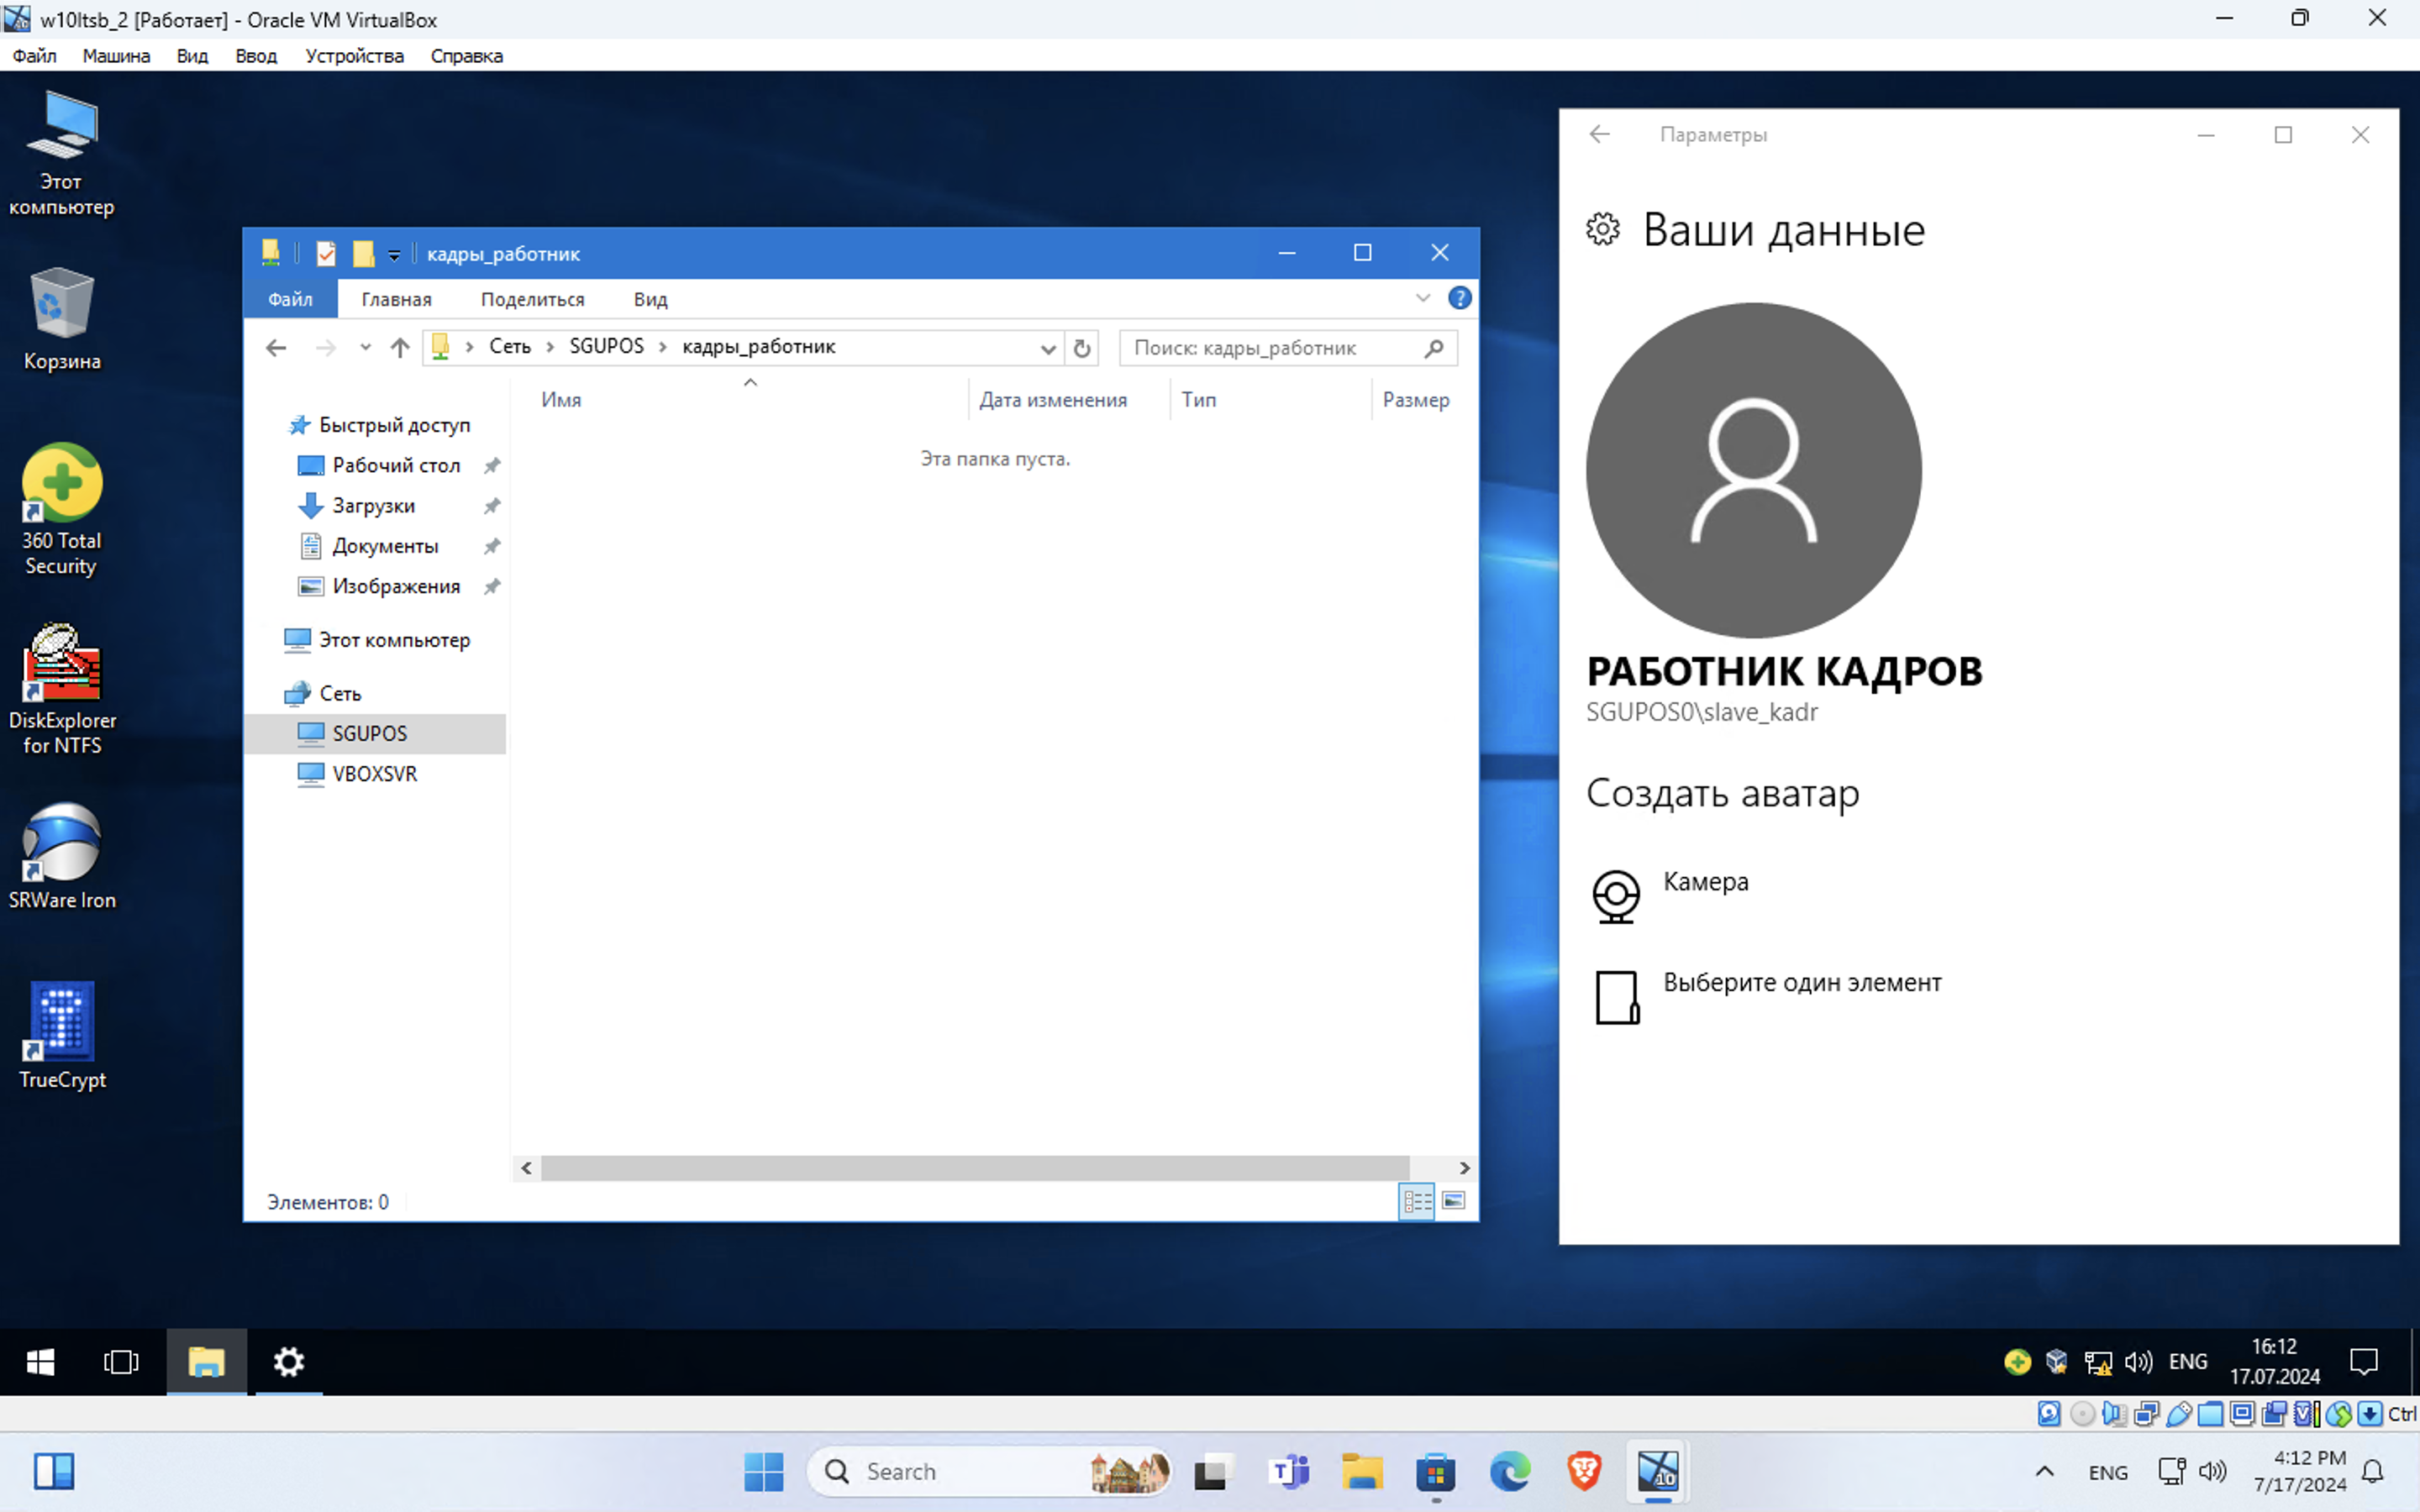
\includegraphics[width=1\textwidth]{pict/prac/28}
  \caption{Работник кадров -> Работник кадров}
  \label{fig:27}
\end{figure}


\begin{figure}[H]
  \centering
  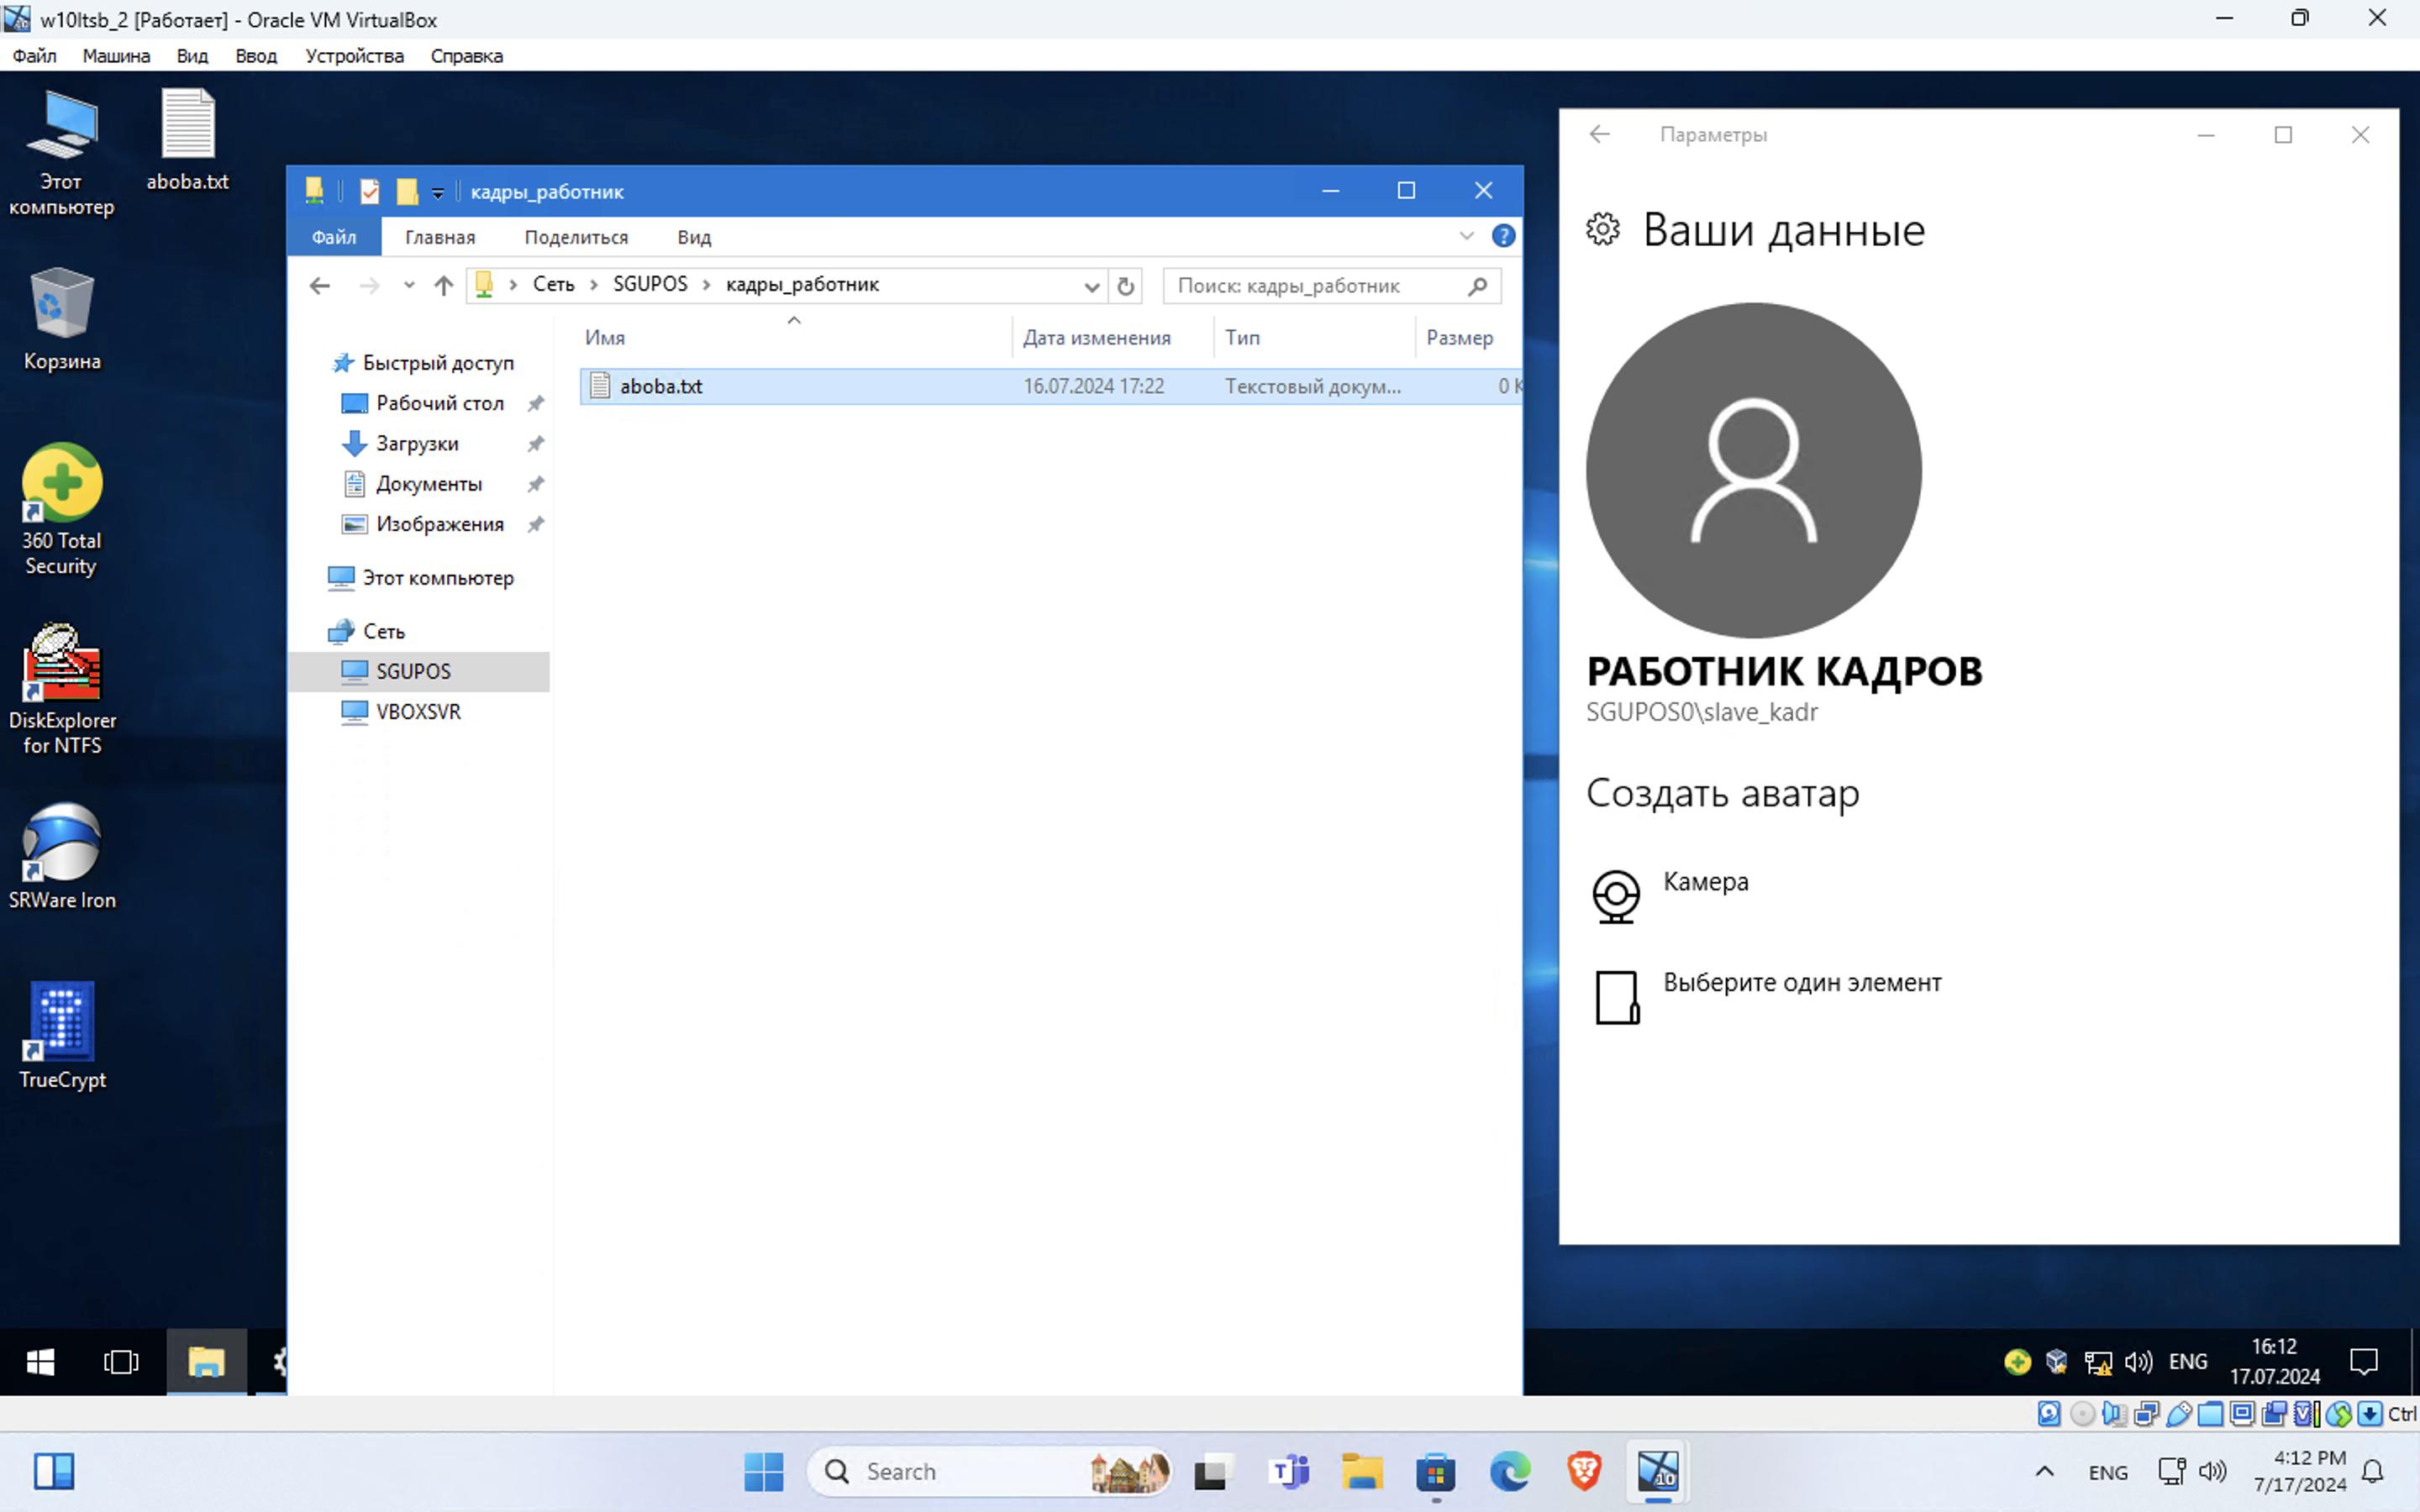
\includegraphics[width=1\textwidth]{pict/prac/29}
  \caption{Может создавать документы}
  \label{fig:28}
\end{figure}

\begin{figure}[H]
  \centering
  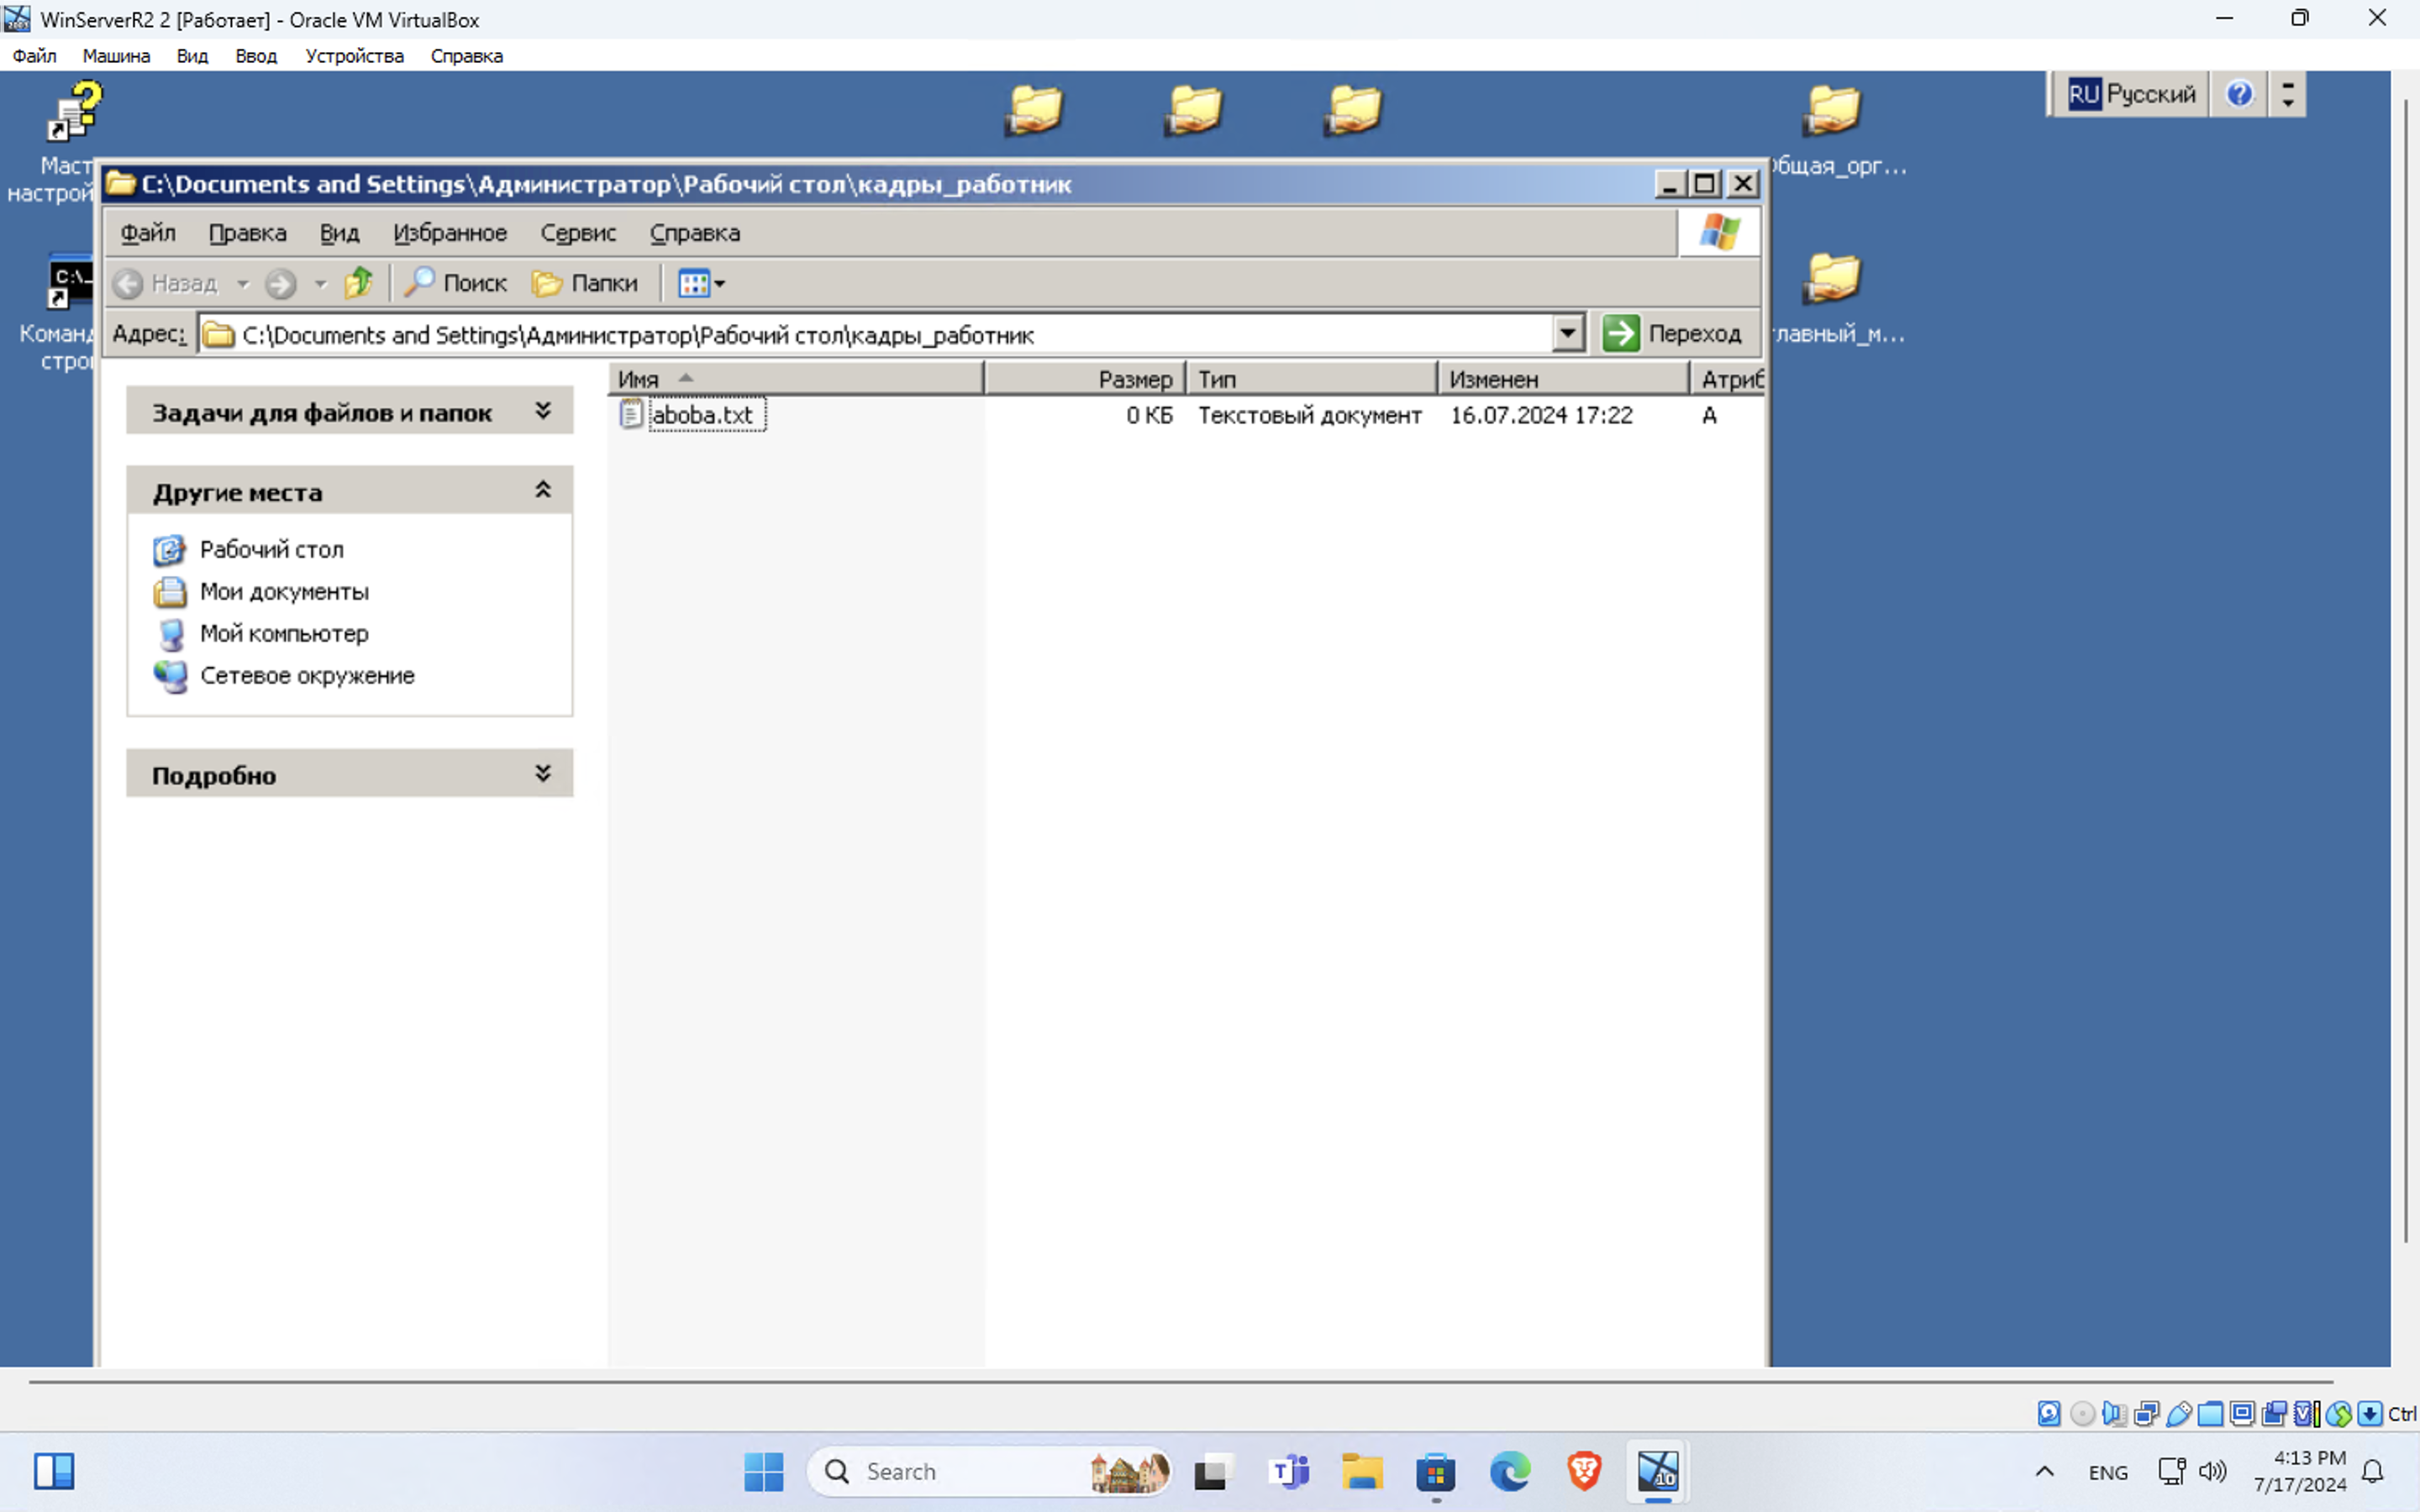
\includegraphics[width=1\textwidth]{pict/prac/30}
  \caption{Созданный работником документ на сервере}
  \label{fig:29}
\end{figure}


\begin{figure}[H]
  \centering
  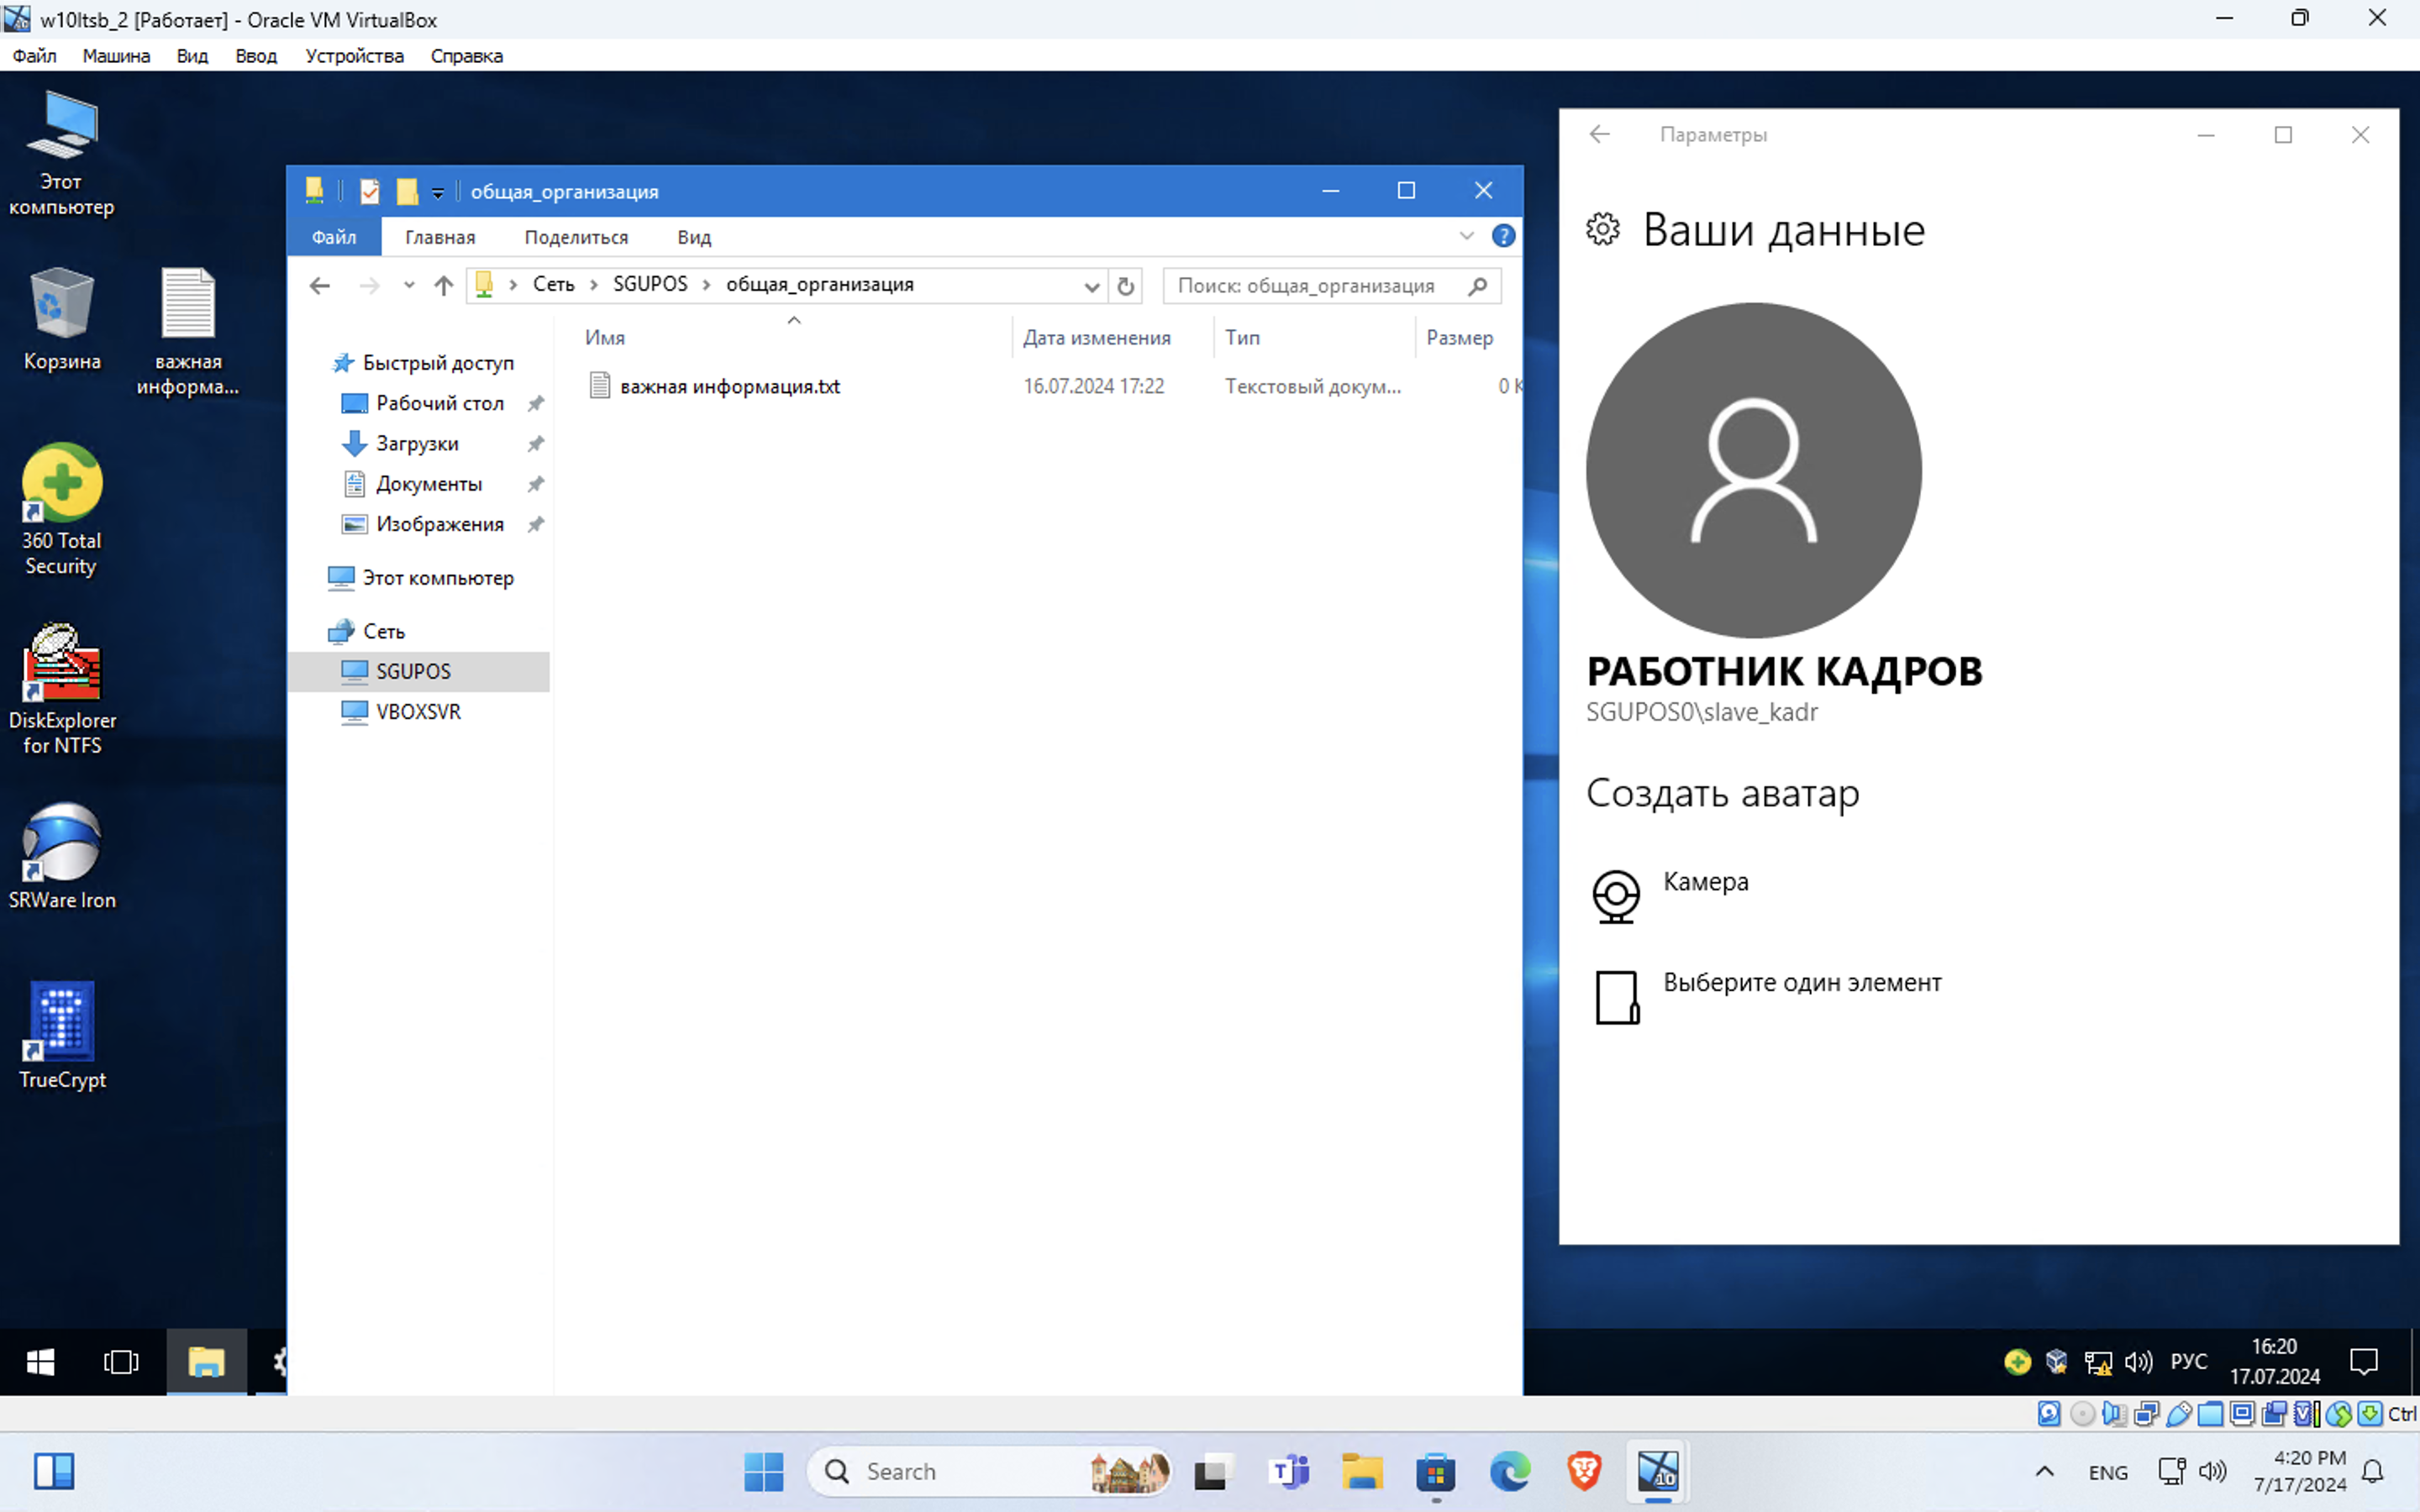
\includegraphics[width=1\textwidth]{pict/prac/33}
  \caption{Создание документа в общей папке}
  \label{fig:32}
\end{figure}

\begin{figure}[H]
  \centering
  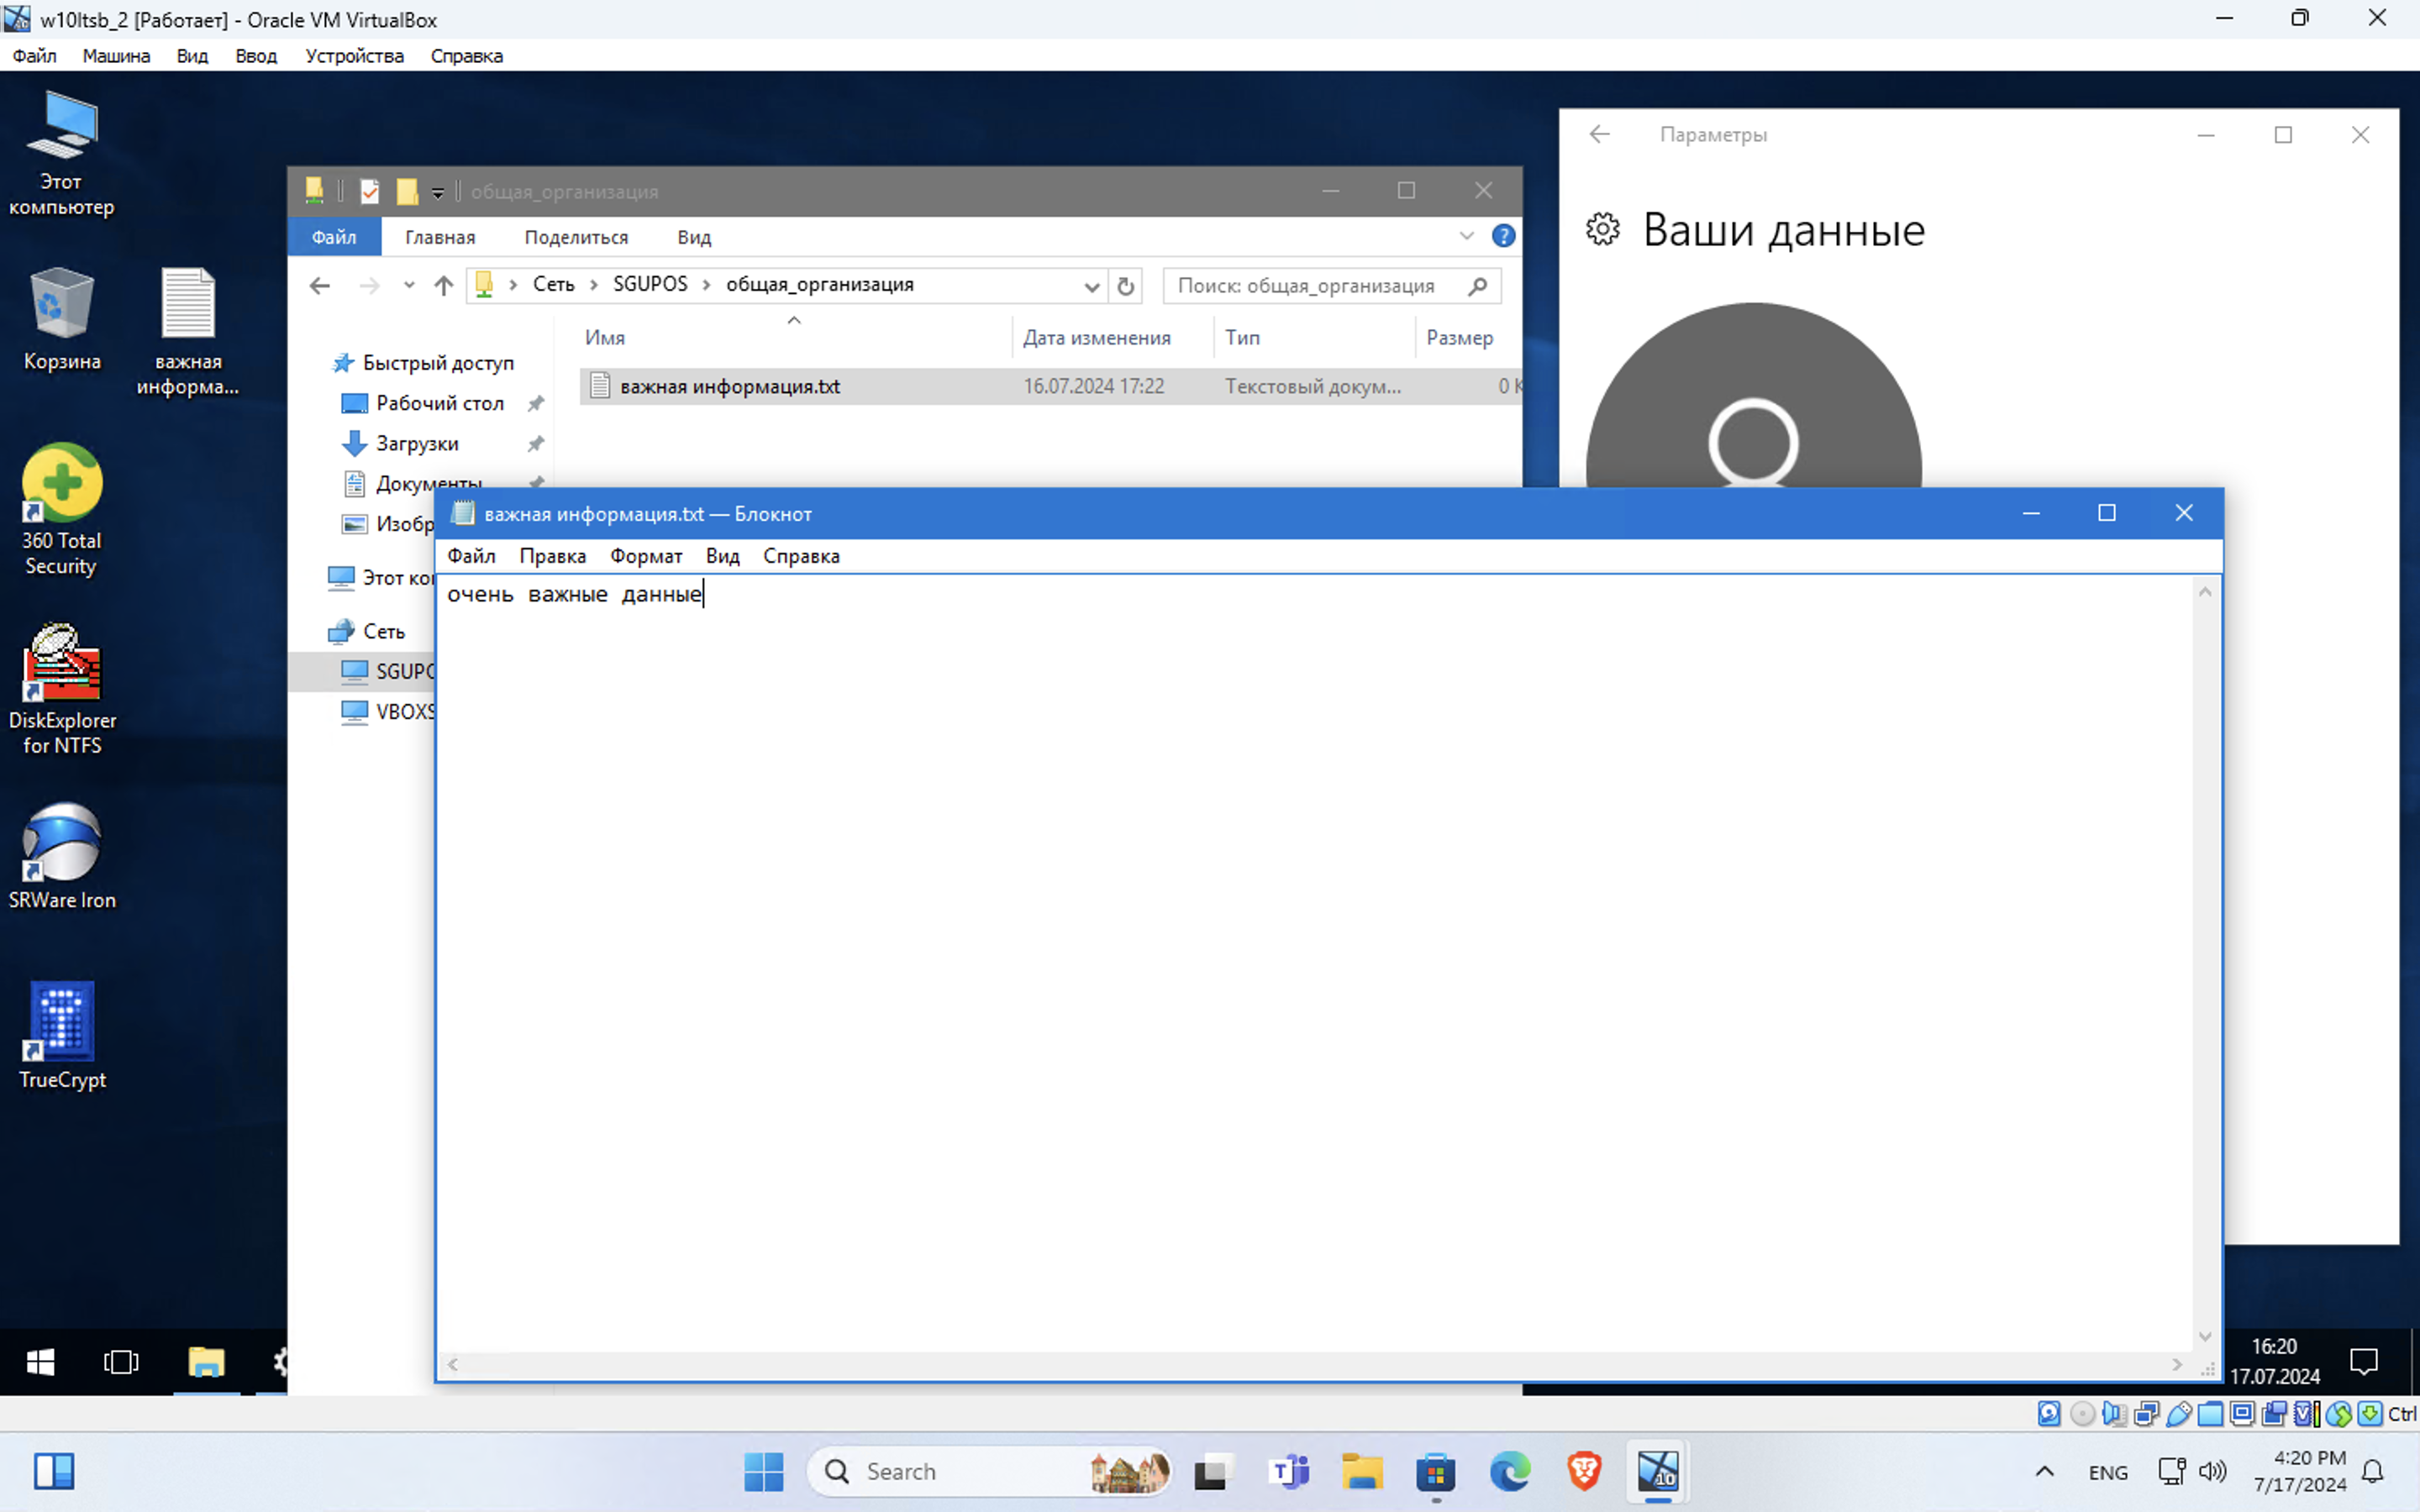
\includegraphics[width=1\textwidth]{pict/prac/34}
  \caption{Создание документа в общей папке}
  \label{fig:33}
\end{figure}

Рассмотрим аккаунт начальника подразделения соискателей и его доступ.
\begin{figure}[H]
  \centering
  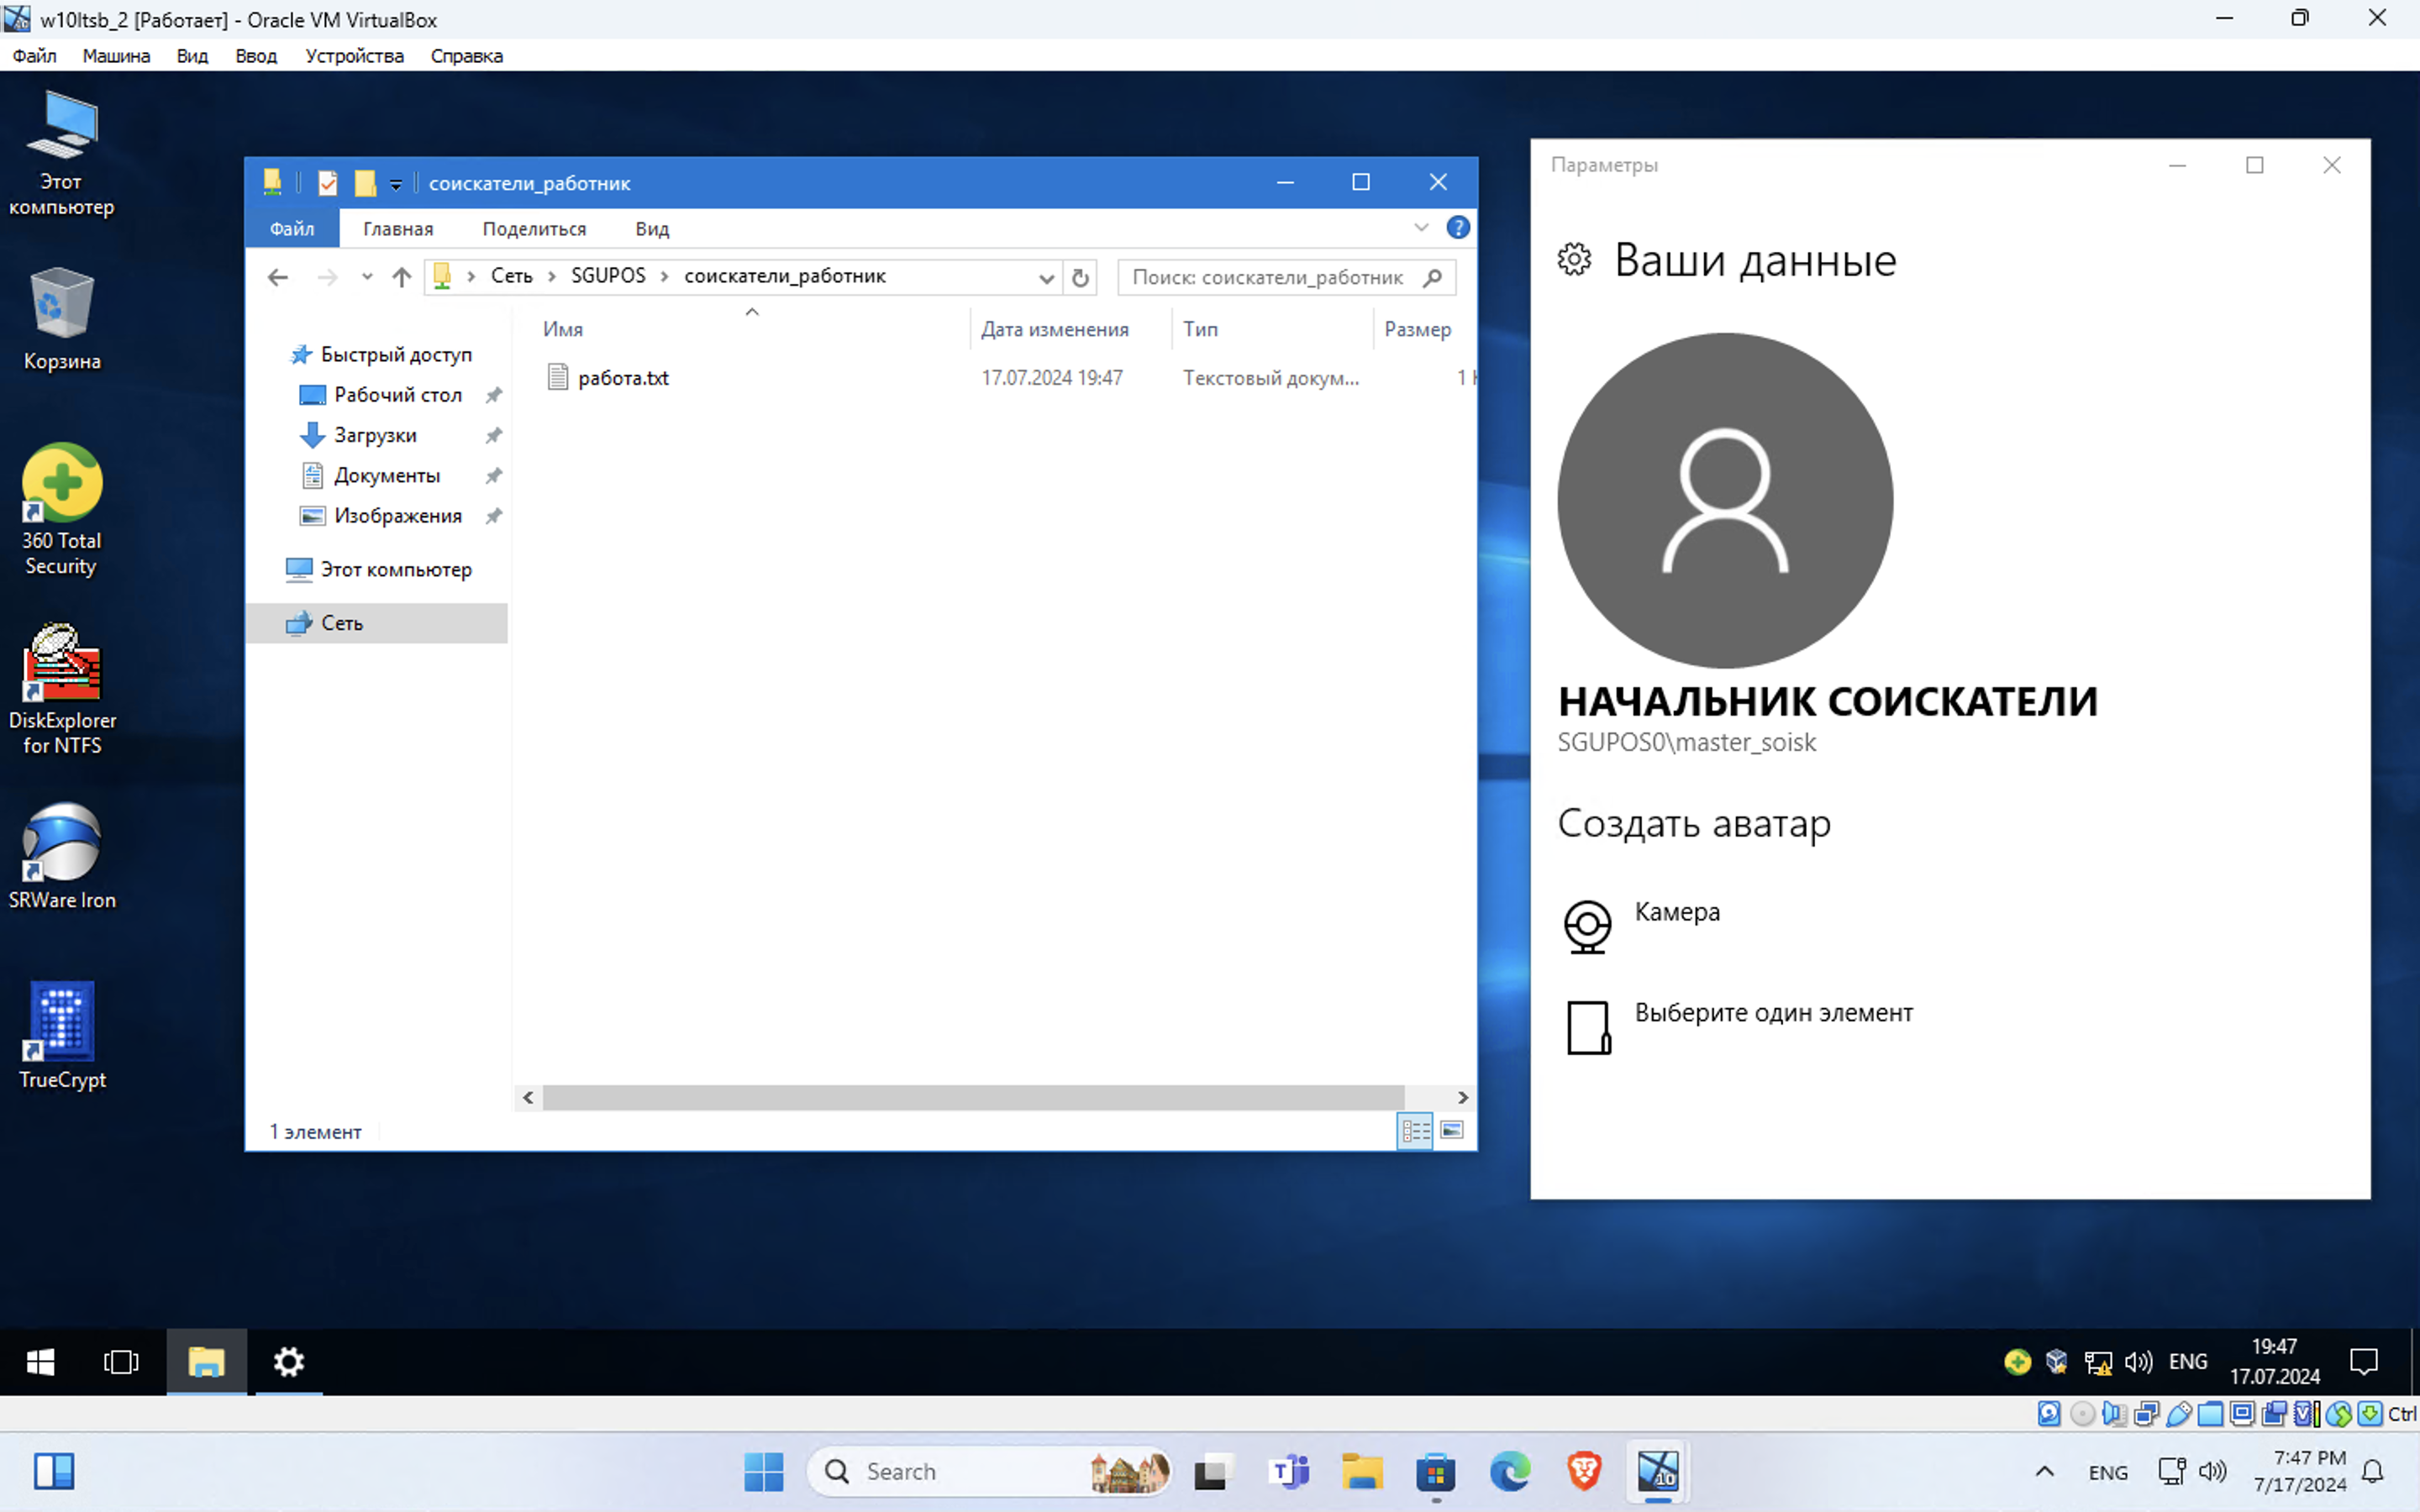
\includegraphics[width=1\textwidth]{pict/prac/35}
  \caption{Начальник соискателей -> Работник соискателей}
  \label{fig:34}
\end{figure}

\begin{figure}[H]
  \centering
  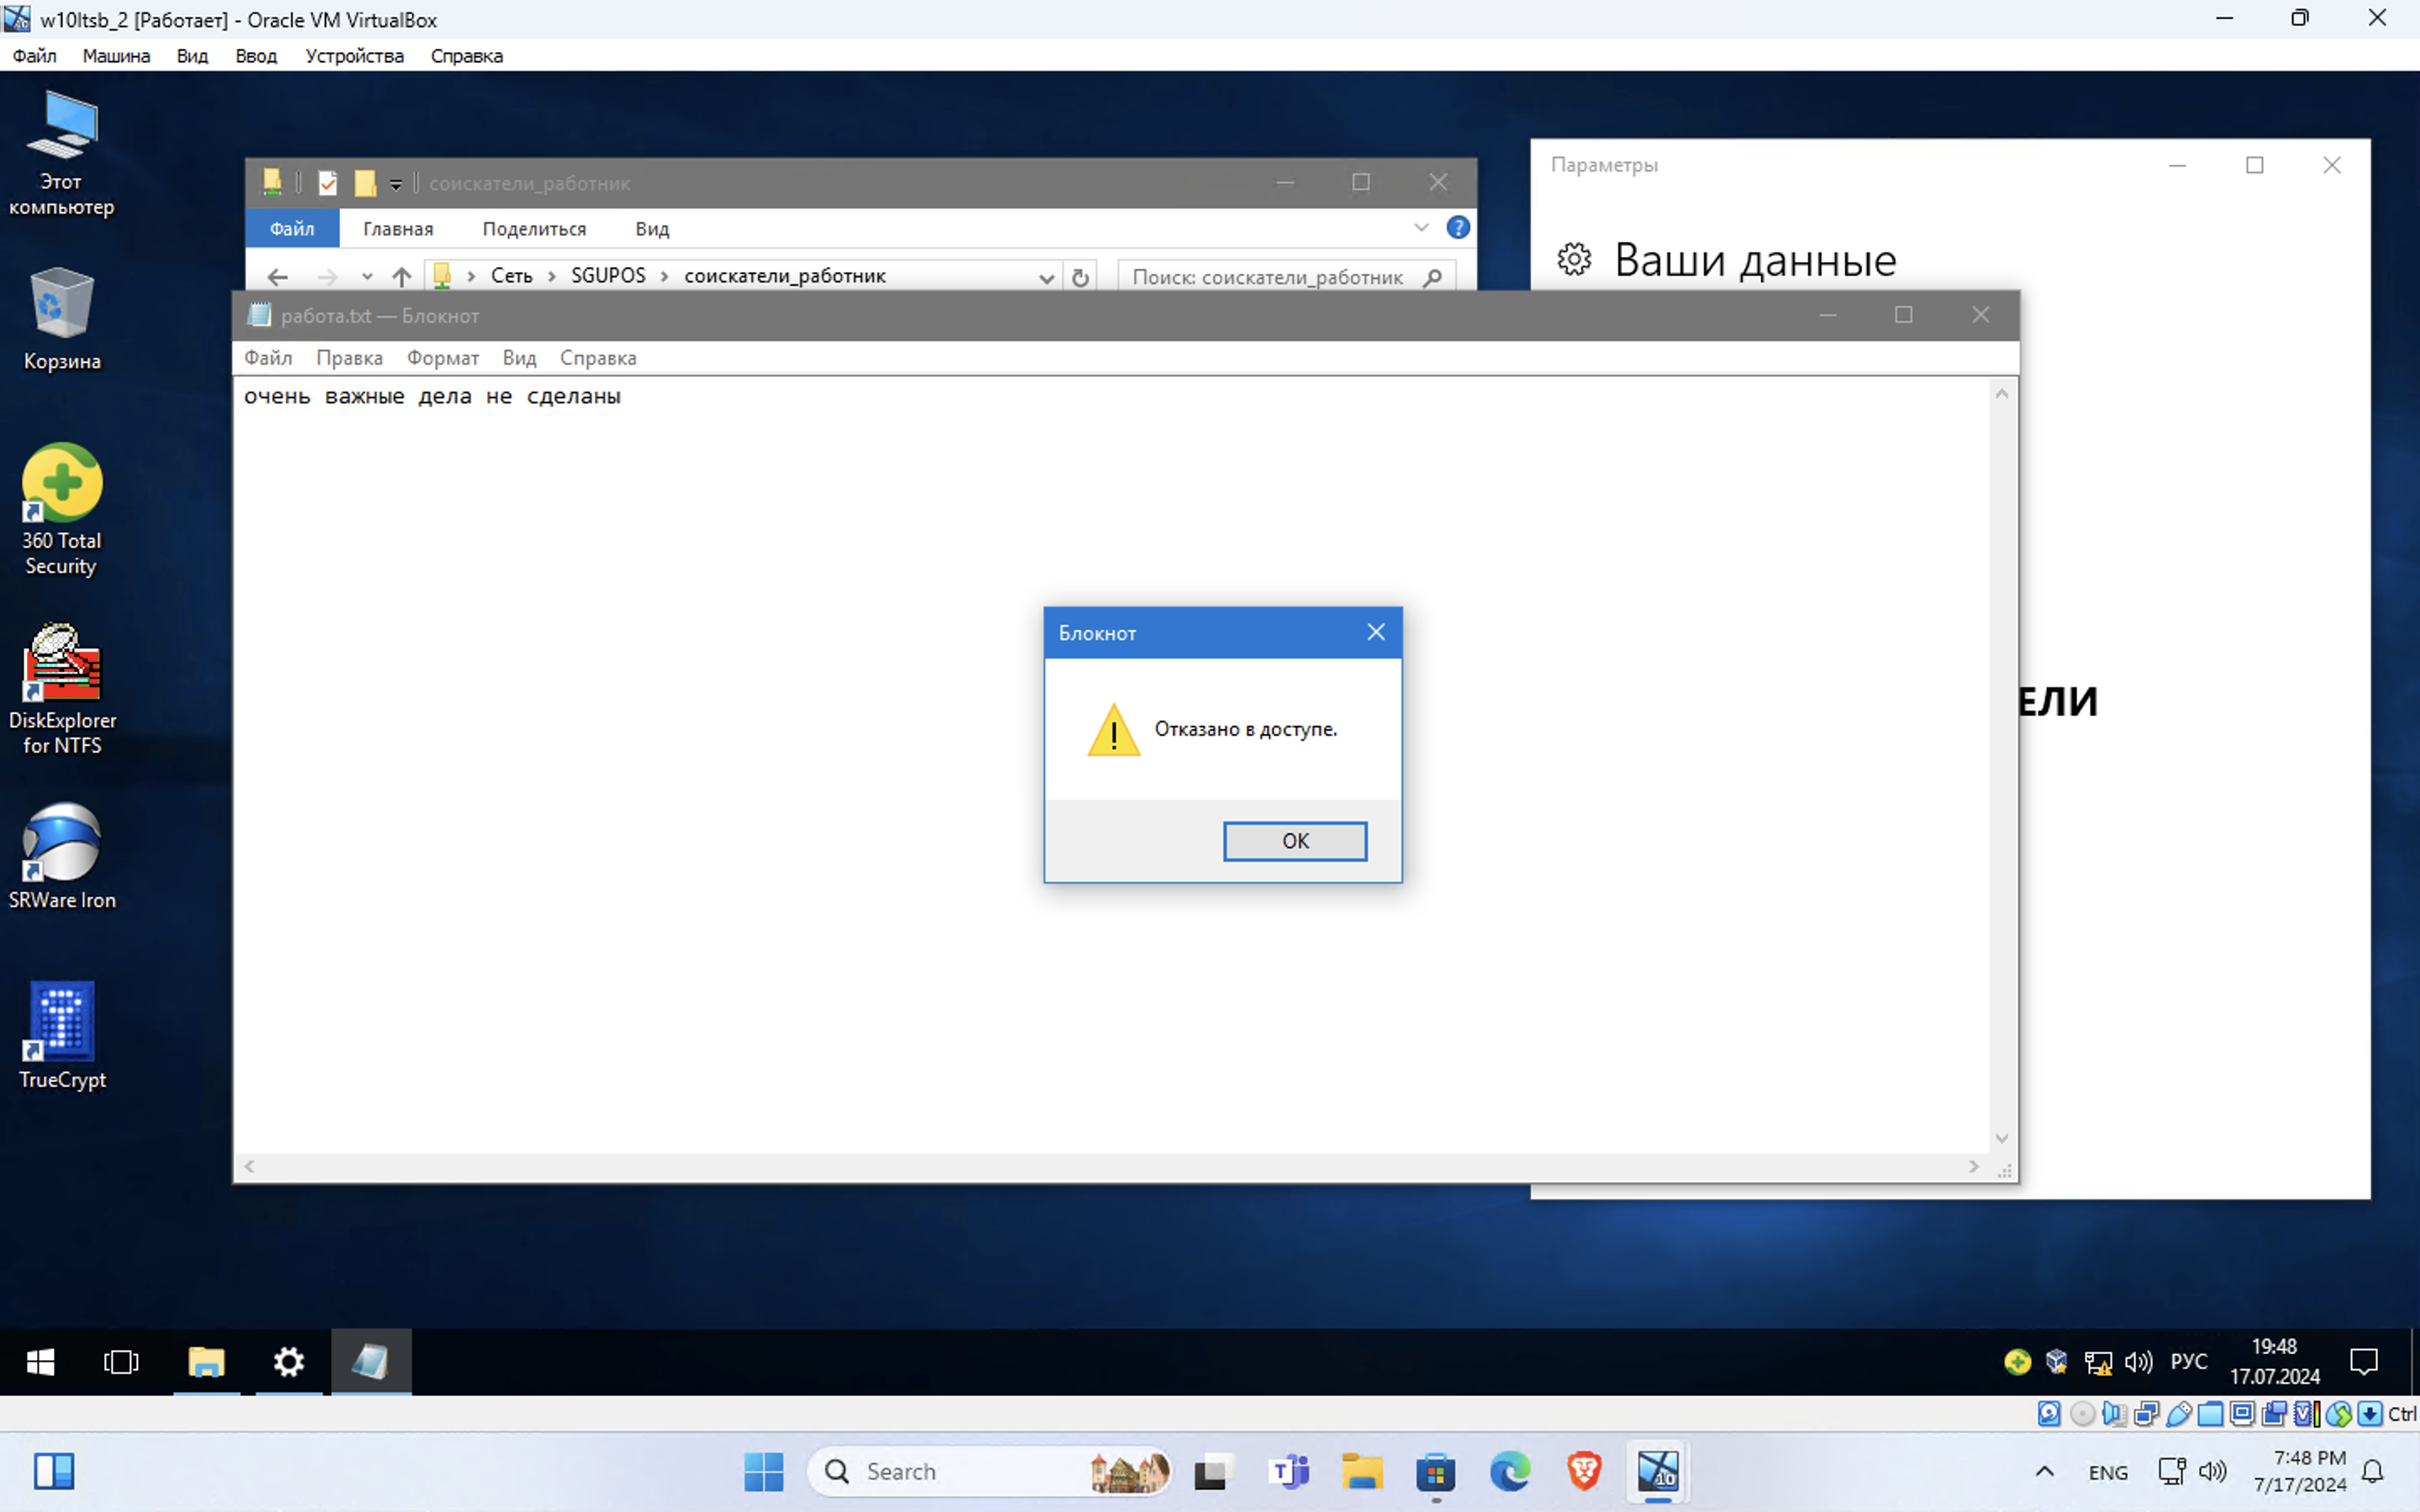
\includegraphics[width=1\textwidth]{pict/prac/36}
  \caption{Изменение документа в папке своего работника}
  \label{fig:35}
\end{figure}

\begin{figure}[H]
  \centering
  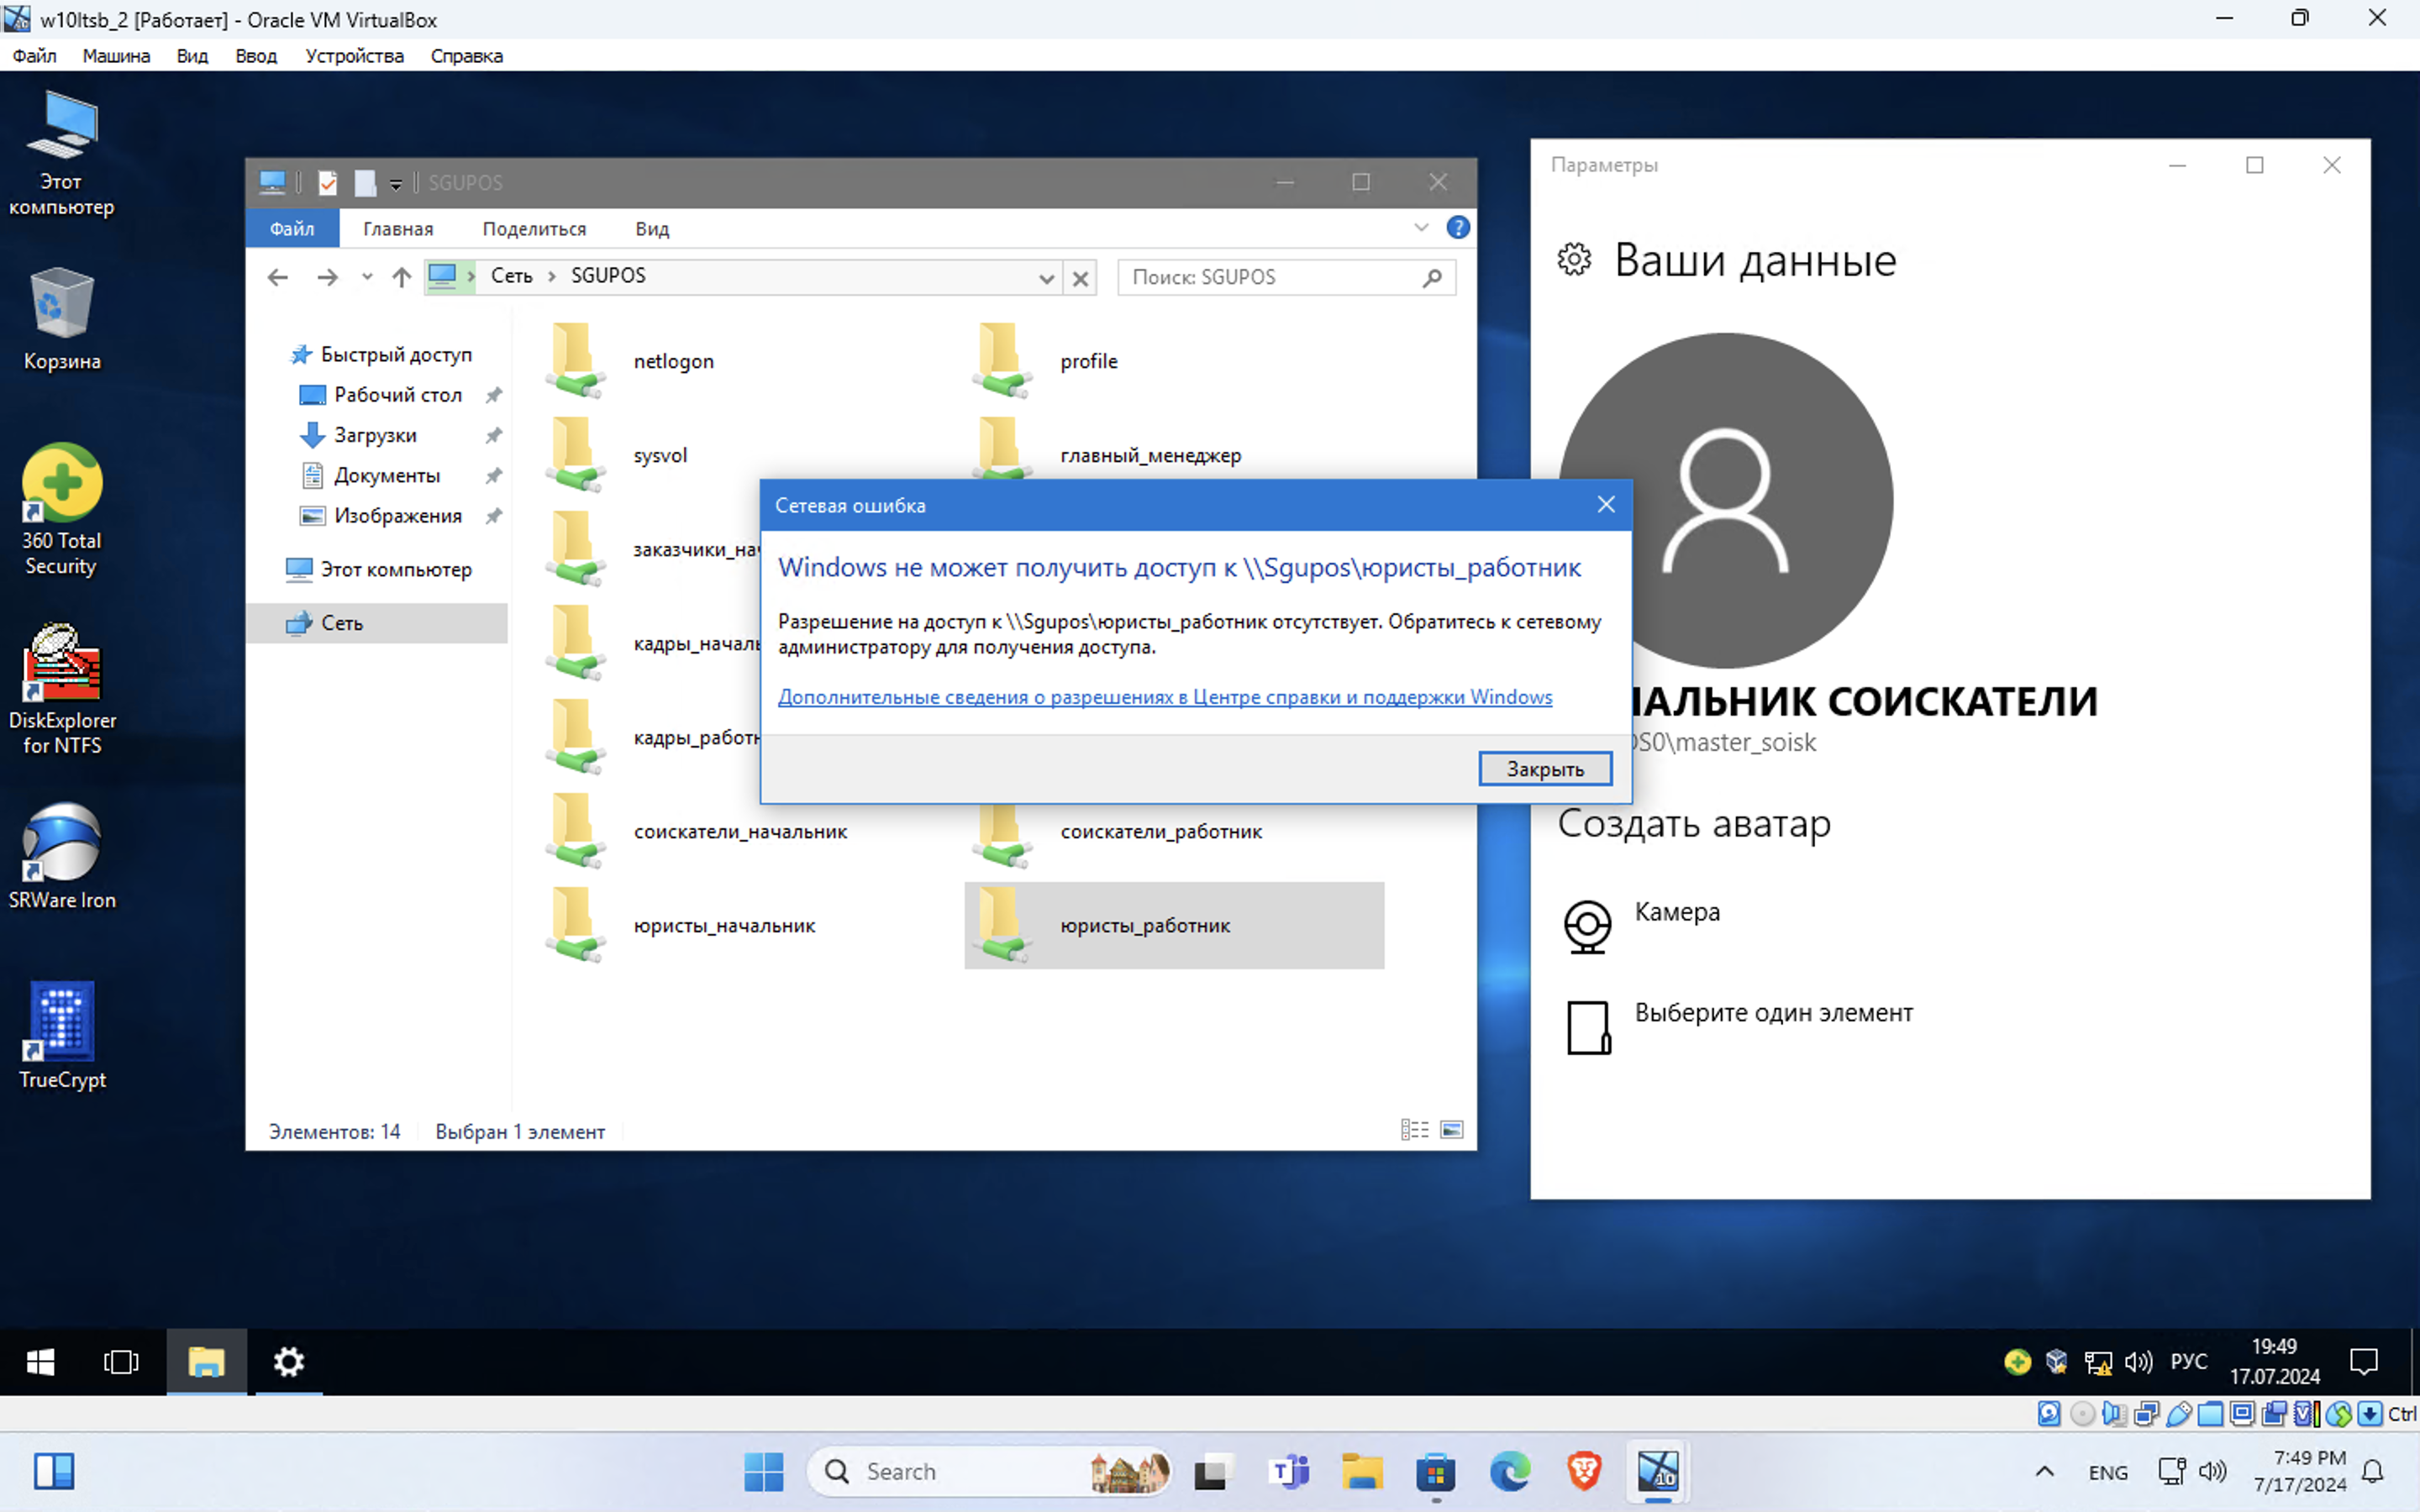
\includegraphics[width=1\textwidth]{pict/prac/39}
  \caption{Начальник соискателей -> Работник юрист}
  \label{fig:38}
\end{figure}

\begin{figure}[H]
  \centering
  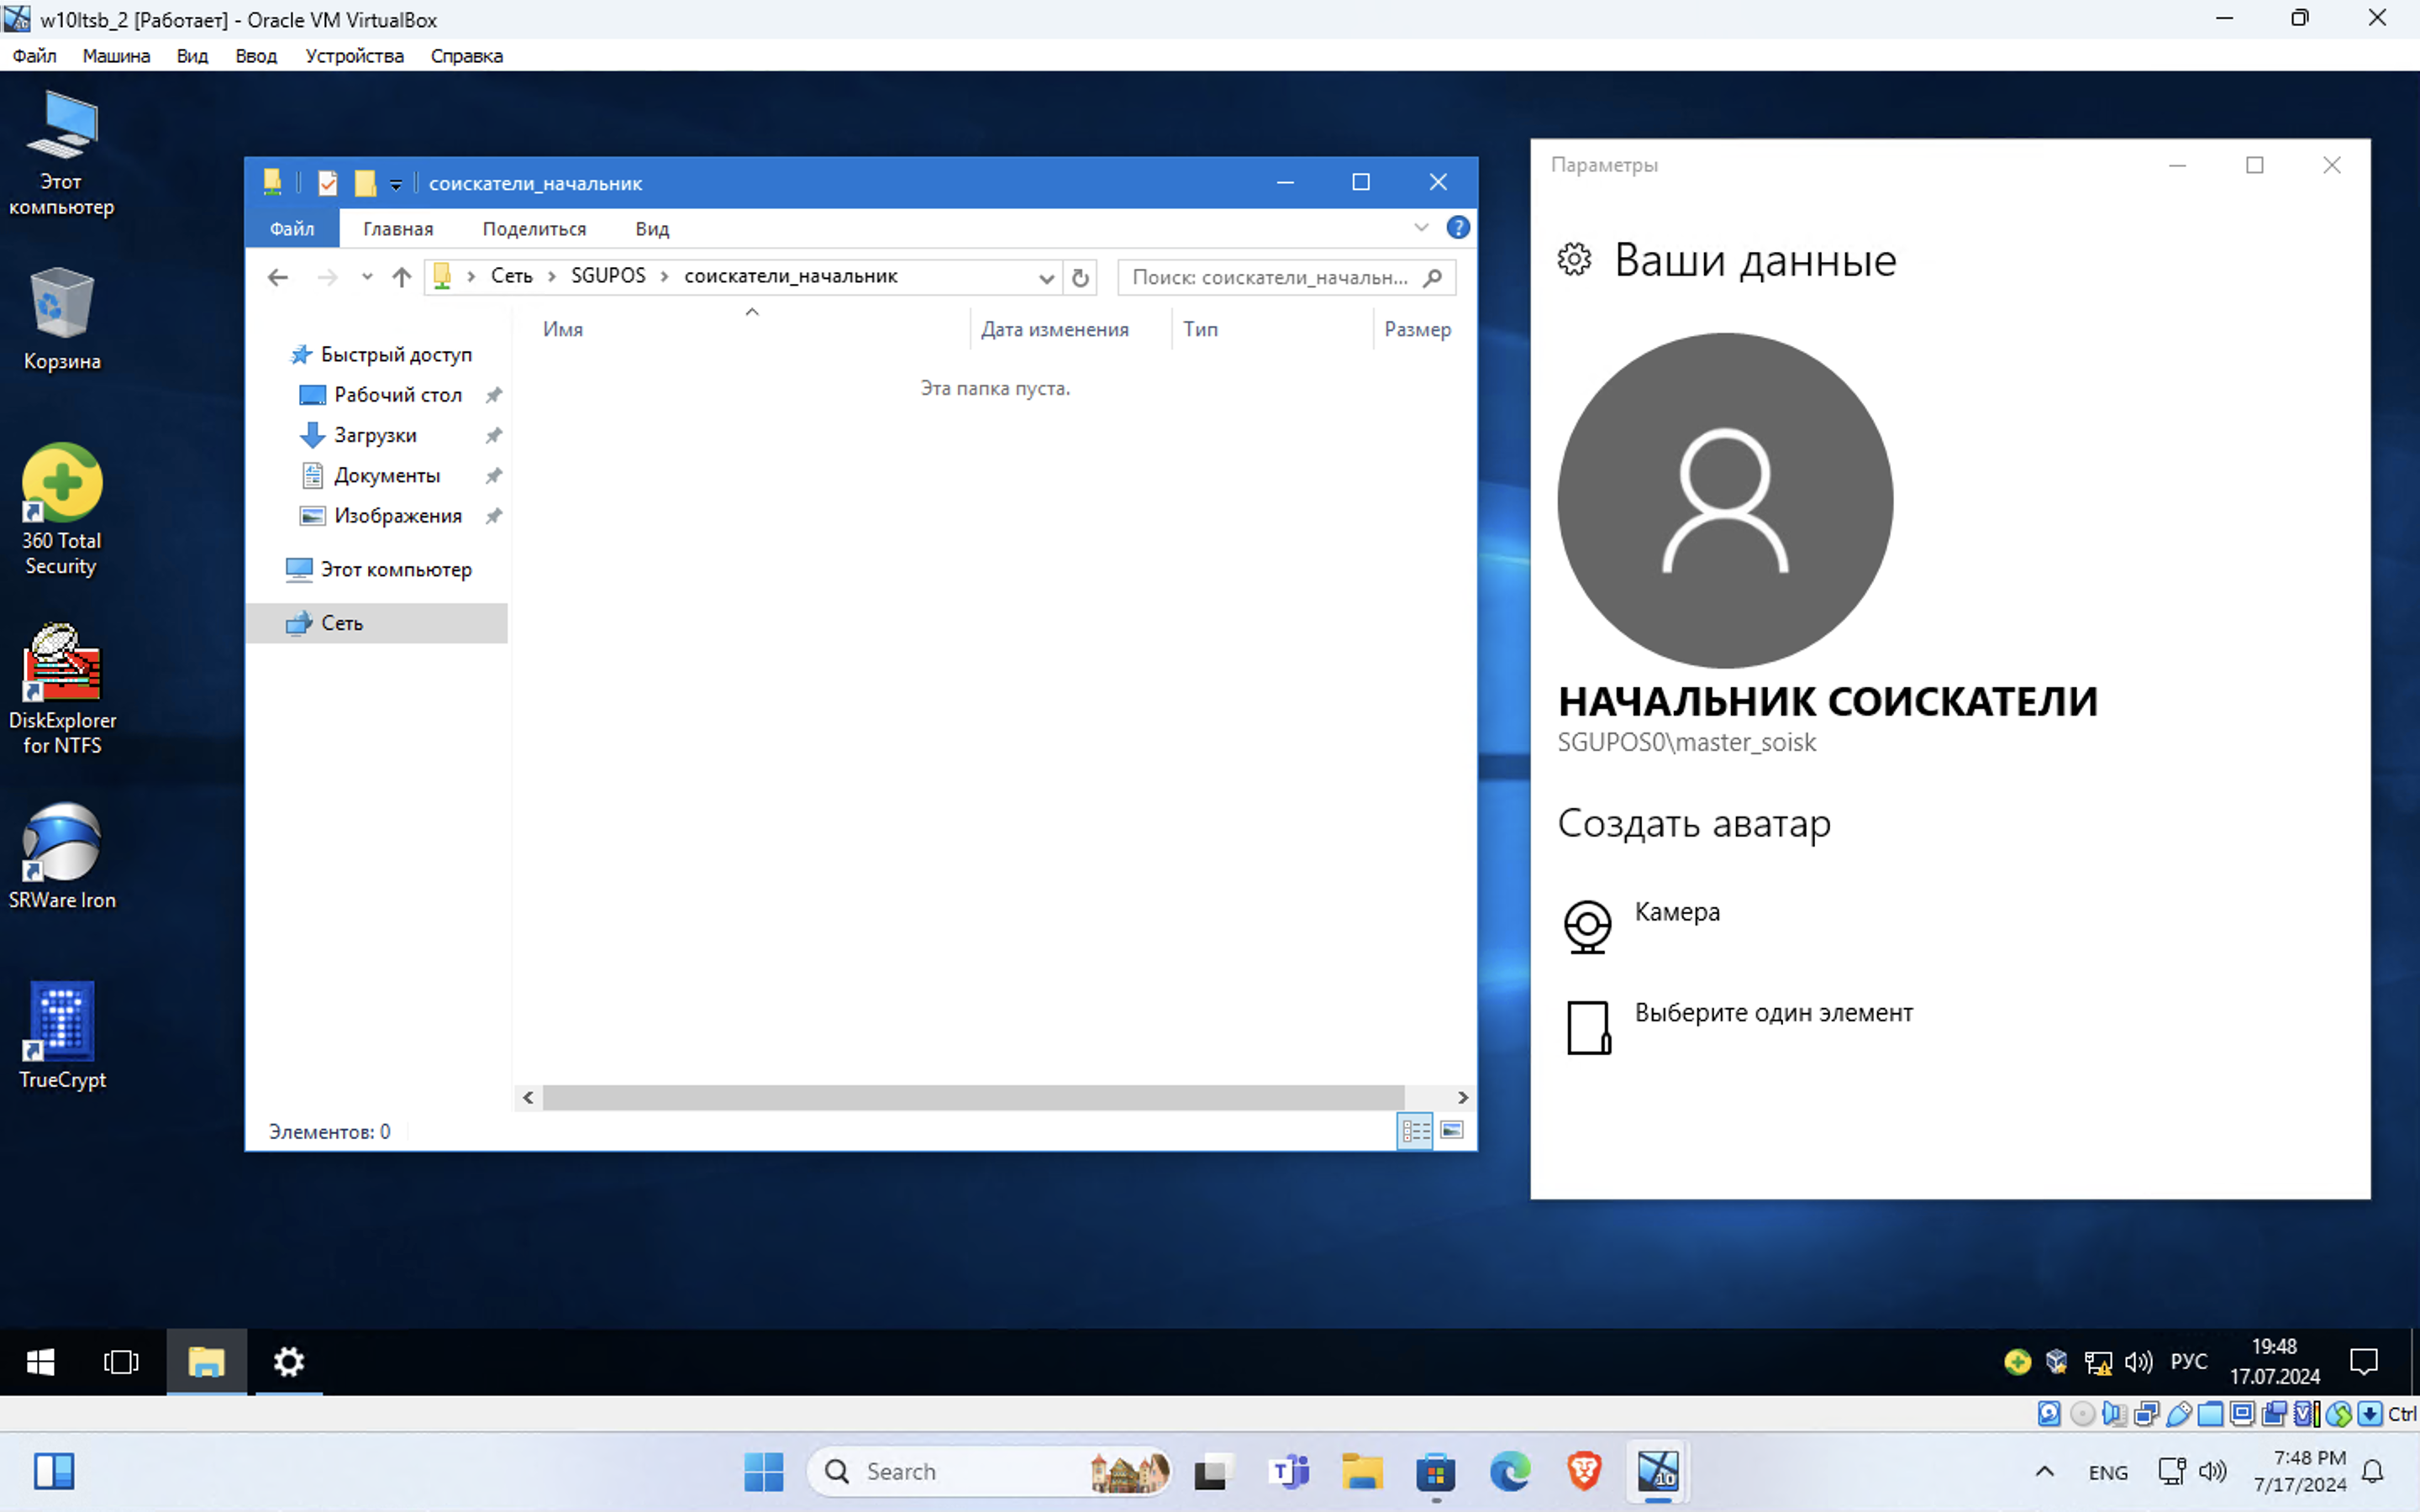
\includegraphics[width=1\textwidth]{pict/prac/37}
  \caption{Начальник соискателей -> Начальник соискателей}
  \label{fig:36}
\end{figure}

\begin{figure}[H]
  \centering
  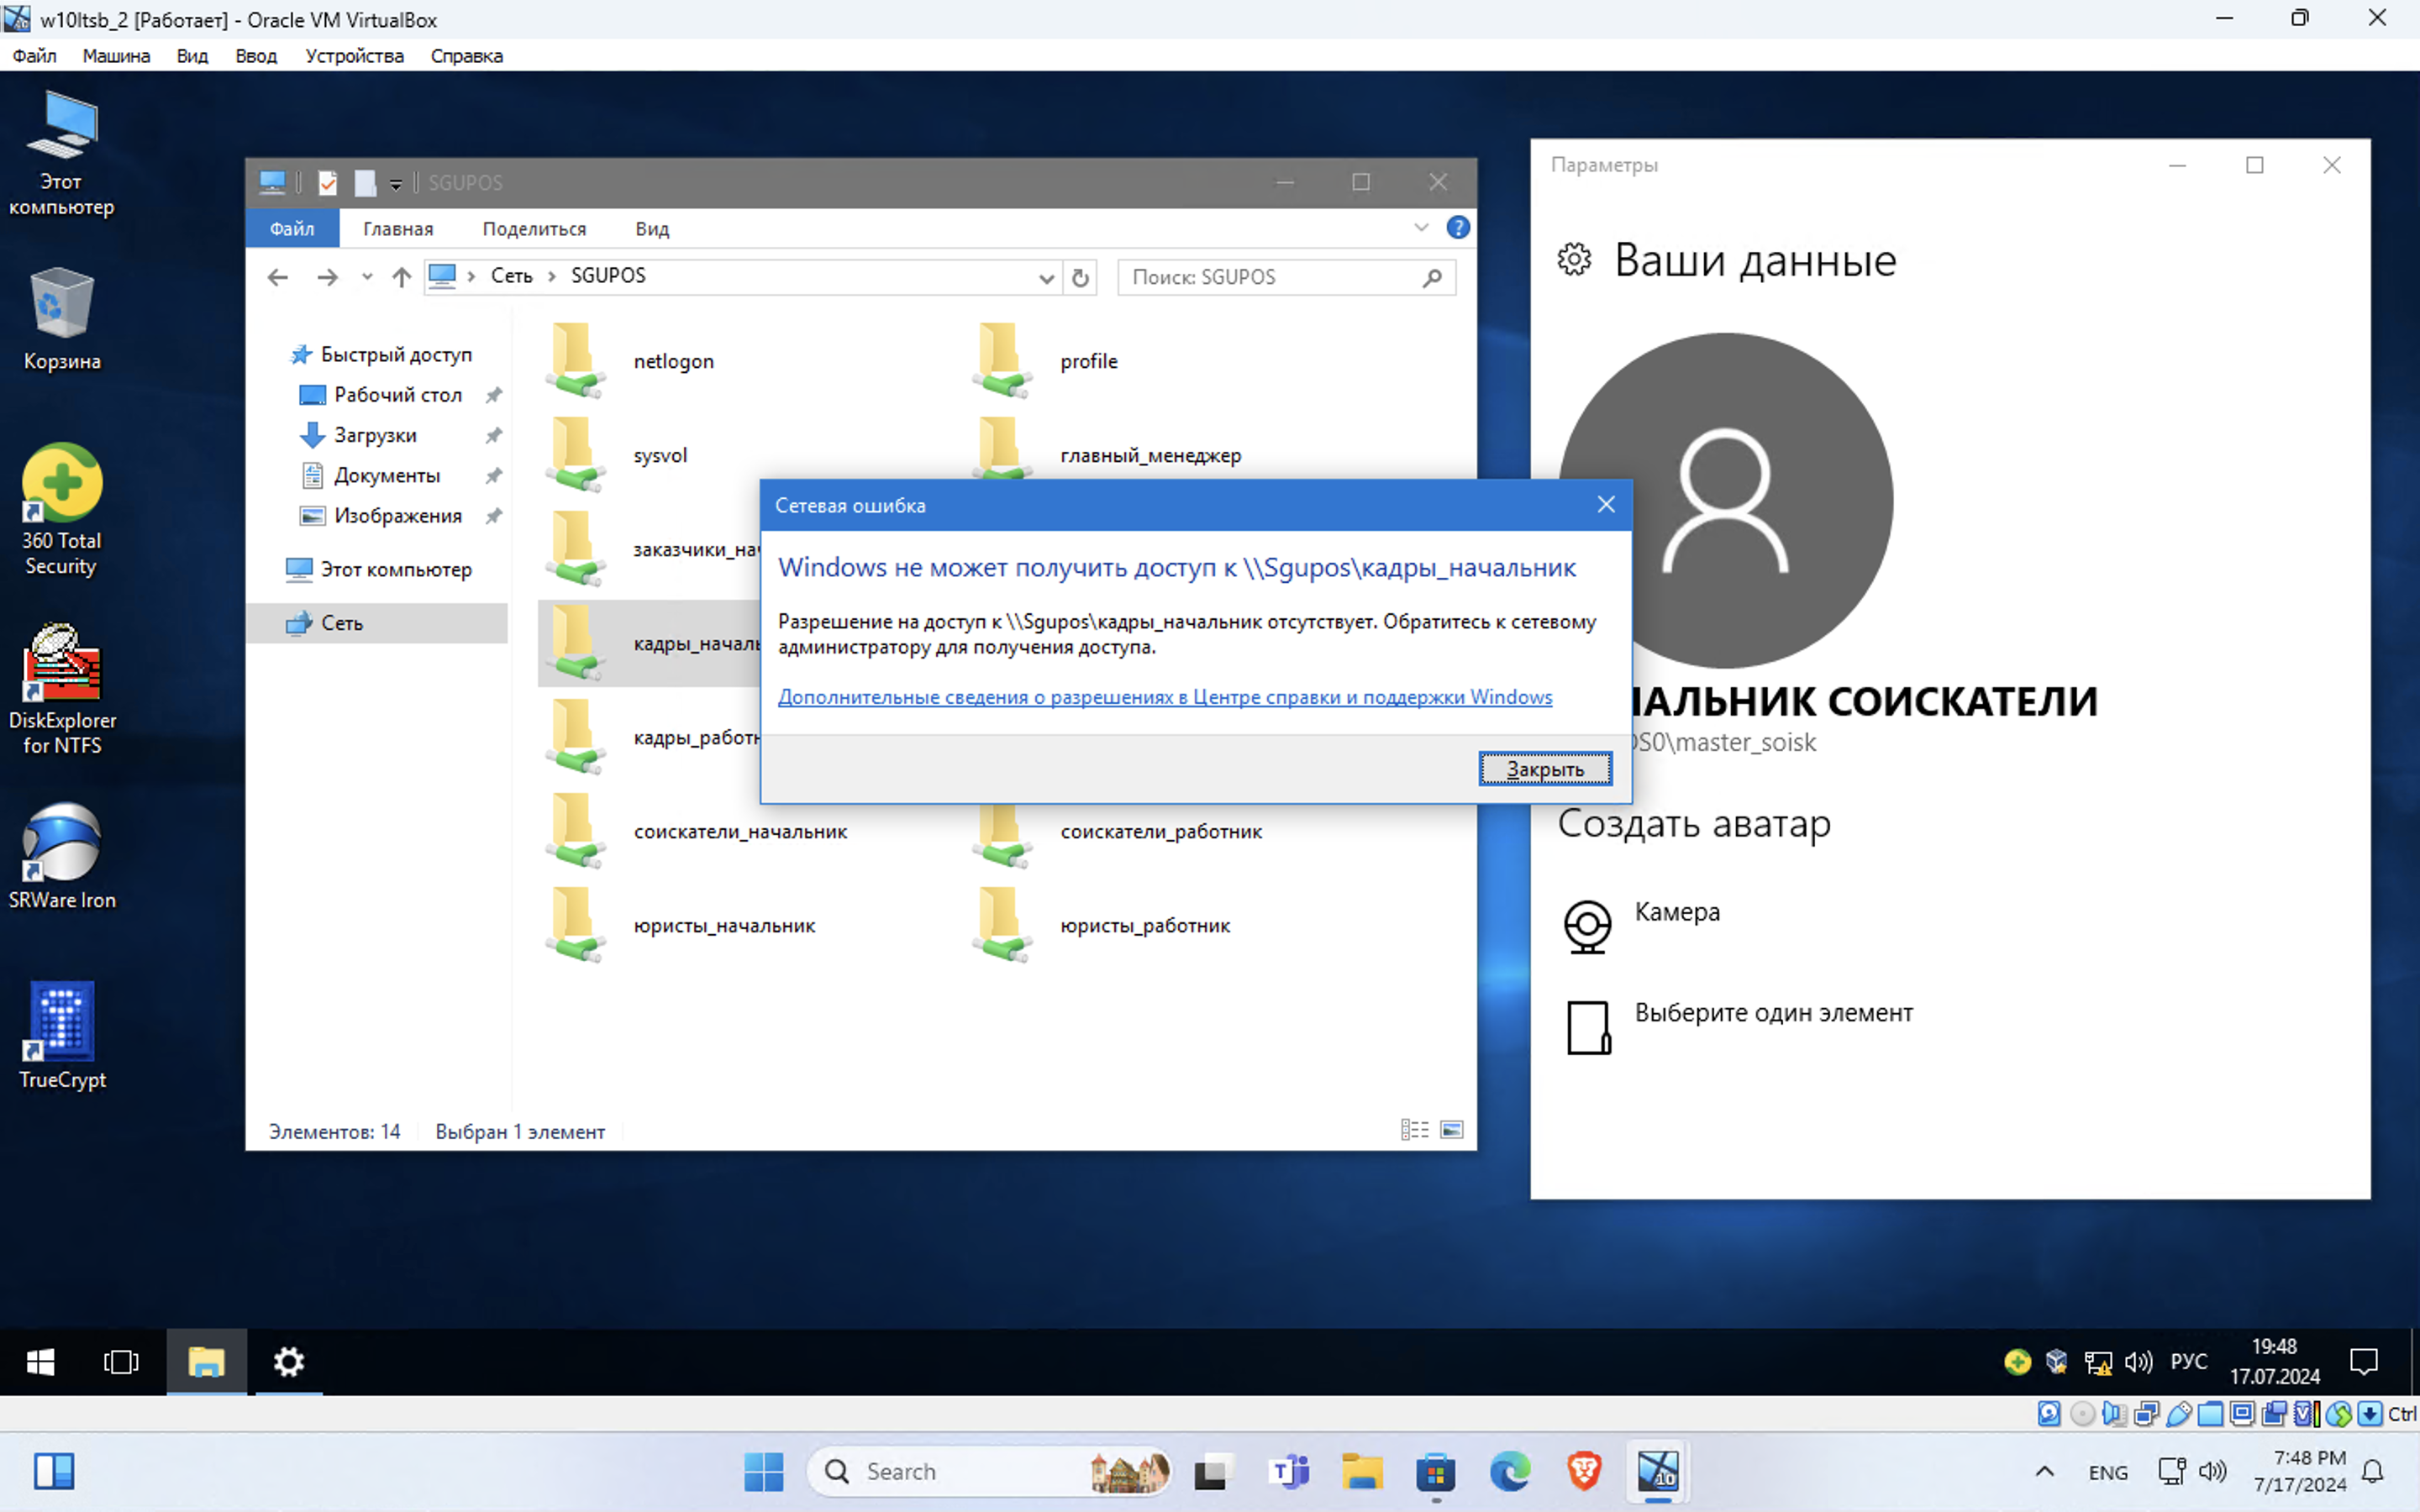
\includegraphics[width=1\textwidth]{pict/prac/38}
  \caption{Начальник соискателей -> Начальник кадров}
  \label{fig:37}
\end{figure}


\begin{figure}[H]
  \centering
  \includegraphics[width=1\textwidth]{pict/prac/40}
  \caption{Начальник соискателей -> Главный менеджер}
  \label{fig:39}
\end{figure}


\begin{figure}[H]
  \centering
  \includegraphics[width=1\textwidth]{pict/prac/42}
  \caption{Доступ к общей папке}
  \label{fig:41}
\end{figure}

\begin{figure}[H]
  \centering
  \includegraphics[width=1\textwidth]{pict/prac/44}
  \caption{Отказ в изменении файла}
  \label{fig:43}
\end{figure}

Аккаунт главного менеджера, который может заглядывать в любые папки.
\begin{figure}[H]
  \centering
  \includegraphics[width=1\textwidth]{pict/prac/45}
  \caption{Главный менеджер -> Начальник соискателей}
  \label{fig:44}
\end{figure}

\begin{figure}[H]
  \centering
  \includegraphics[width=1\textwidth]{pict/prac/46}
  \caption{Изменять папку он также не может}
  \label{fig:45}
\end{figure}

\begin{figure}[H]
  \centering
  \includegraphics[width=1\textwidth]{pict/prac/47}
  \caption{Главный менеджер -> Главный менеджер}
  \label{fig:46}
\end{figure}




% \addcontentsline{toc}{section}{\hspace{15mm}ЗАКЛЮЧЕНИЕ}
\section*{ЗАКЛЮЧЕНИЕ}
\addcontentsline{toc}{section}{ЗАКЛЮЧЕНИЕ}
Рассмотренные отечественные решения АПМДЗ, обладают широким комплексом 
полезных функций, который обеспечивает защиту не только на уровне загрузки ОС, 
но также и после. Данные модули к тому же имеют сертификат ФСТЭК, 
а некоторые внесены в реестр отечественного ПО, что позволят поднять уровень информационной 
безопасности в компании. 

Также была реализована настройка учетных записей в домене организации рекрутингового агентства,
и соответственно реализованы требования к данной системе, выполнение которых также было проверено.


\section*{СПИСОК ИСПОЛЬЗОВАННЫХ ИСТОЧНИКОВ}
\addcontentsline{toc}{section}{СПИСОК ИСПОЛЬЗОВАННЫХ ИСТОЧНИКОВ}
% \input{sections/istoch.tex}
% \section{Приложение А}
% \section{Приложение Б}
% \begin{thebibliography}{99}
  \bibitem{Andriyanov} Андриянов В., ОБЕСПЕЧЕНИЕ ИНФОРМАЦИОННОЙ БЕЗОПАСНОСТИ БИЗНЕСА, M.: Паблишер, 2010. -235 с.
  \bibitem{Gruzdev} Груздев С., Сабанов А., ``Вопросы идентификации и аутентификации при разработке мультиаппликационных карт'', [Электронный ресурс] -  URL:\\ https://www.aladdin-rd.ru/company/pressroom/articles/voprosy\_identifikacii\_\\i\_autentifikacii\_pri\_razrabotke\_multiapplikacionnyh\_kart, дата обращения 26.05.2024, Яз. Рус.
  \bibitem{Korzhov} Коржов В., ``Пароль на минуту'', [Электронный ресурс] / URL: \\https://www.osp.ru/cw/2005/01/84855/, дата обращения 26.05.2024, Яз. Рус.
  \bibitem{Sabanov} Сабанов А., ``О технологиях идентификации и аутентификации'', [Электронный ресурс] / URL: https://www.aladdin-rd.ru/company/pressroom/articles/o\_\\tehnologiah\_identifikacii\_i\_autentifikacii, дата обращения  26.05.2024, Яз. Рус.
  \bibitem{Fisenko} Фисенко Л., ``Новое лицо киберпреступности'', [Электронный ресурс] / URL:\\https://www.itweek.ru/infrastructure/article/detail.php?ID=71779, дата обращения 24.05.2024, Яз. Рус.
  \bibitem{Fiso} PHP Framework List: An Ultimate Guide to 102 PHP Frameworks for Web Developers, [Электронный ресурс] / URL: https://www.temok.com/blog/php-framework-list/, дата обращения 26.05.2024.
  \bibitem{Белик} Венц К., ``Безопасность ASP.NET Core'', пер. с англ. Д. А. Беликова, г. Москва, Издательство ДМК Пресс, 2023 г., Яз. Рус.
  \bibitem{Юртанова} Юртанова Е., Разработка web-приложений с использованием языка PHP / Е. М. Юртанова // Учебный эксперимент в образовании. 2011. 47 с.
  \bibitem{Laravel} ``Почему стоит выбрать Laravel для веб-разработки в 2022'', [Электронный ресурс] / URL: https://firecode.ru/blog/pochemu-stoit-vybrat-laravel-dlya-veb-razrabotki-v-2022, дата обращения 25.05.2024.
  \bibitem{Захаров} Захаров В., ``Проблемы выбора языков программирования при разработке кроссплатформенных приложений'', [Электронный ресурс] /  URL: https://cyberleninka.ru/article/n/problemy-vybora-yazykov-programmirovaniya-pri-razrabotke-krossplatformennyh-prilozheniy, дата обращения 25.05.2024.
\end{thebibliography}
% Неправильно оформлена библиография, нужен бибтех

\end{document}